\documentclass[12pt]{report}

%%
% to enumerate subsubsection
%%
\addtocounter{tocdepth}{3}
\setcounter{secnumdepth}{3}
% \usepackage{tgtermes}
\usepackage[a4paper, margin=1in]{geometry}
\usepackage[T1]{fontenc}
\usepackage[breaklinks,hidelinks]{hyperref}
\usepackage[utf8]{inputenc}
\usepackage{graphicx} 
\usepackage{tikz}
\usepackage{amsmath, amssymb}
% \usepackage{indentfirst}
% \usepackage{cite}
\usepackage{natbib}
\usepackage[nameinlink,noabbrev]{cleveref}
\usepackage[capposition=top]{floatrow}
\usepackage{float}
\usepackage{caption}
\usepackage{xfrac}
\usepackage{braket}
\usepackage[toc,page]{appendix}
\usepackage{tabularx}
\usepackage{adjustbox}
\usepackage{multirow}
\usepackage{arydshln}
% \usepackage{hyperref}
% \usepackage{physics}

%%
% to enumerate subsubsection
%%
\addtocounter{tocdepth}{3}
\setcounter{secnumdepth}{3}

% Snippet
\newcommand{\BSM}{Black--Scholes--Merton }
\newcommand{\lnorm}{log-normally }
\newcommand{\bmotion}{Brownian Motion }
\newcommand{\stvar}{stochastic variable }
\newcommand{\wienpro}{Wiener process }
\newcommand{\markpro}{Markov process }

% 
% Bunch of new commands
% 
% brownian motion
\newcommand{\dBm}{dW\left(t\right)}
\newcommand{\dpoiss}{dq\left(t\right)}
\newcommand{\DBm}{\delta{W\left(t\right)}}
\newcommand{\Bm}{W\left(t\right)}
\newcommand{\Bmsub}[1]{W_{#1}\left(t\right)}
\newcommand{\Dt}{\Delta t} 
\newcommand{\Bmdist}{\DBm \sim N \left( 0, \Dt \right)}
\newcommand{\ft}{f\left(t, \Bm \right)}
\newcommand{\E}{\mathop{\mathbb{E}}}
\newcommand{\ct}{c\left(t, x\right)}
\newcommand{\dcx}{\frac{\delta\ct}{\delta x}}
\newcommand{\dciix}{\frac{\delta^2\ct}{\delta x^2}}
\newcommand{\dct}{\frac{\delta\ct}{\delta t}}
\newcommand{\N}[1]{N\left(#1\right)}
\newcommand{\dsub}[1]{d_{#1}\left(\Dt, x\right)}
\newcommand{\call}[2]{c\left( #1, #2\right)}
% % about stock
\newcommand{\St}{S\left(t\right)}
\newcommand{\Vt}{V\left(t\right)}
\newcommand{\Si}{S\left(0\right)}
\newcommand{\dSt}{dS\left(t\right)}
\newcommand{\DSt}{\Delta S\left(t\right)}
\newcommand{\dSr}{\frac{\dSt}{\St}}
\newcommand{\DSr}{\frac{\DSt}{\St}}
\newcommand{\Scontinuous}{\St = \Si e^{\sigma\Bm + \left(\alpha - \frac{1}{2 \sigma^2}\right)t}}
\newcommand{\Itobmdiff}{d\ft = \left[\frac{\partial \ft }{\partial t} + \frac{1}{2} \frac{\partial ^2\ft }{\partial x^2}\right]dt + \frac{\partial \ft}{\partial x} \dBm}
\newcommand{\Scontinousdiff}{d\St &= \alpha \St dt + \sigma \St \dBm}
\newcommand{\Scontinuousrate}{\dSr &= \alpha dt + \sigma \dBm}
 \newcommand{\Sdiscretediff}{d\St &= \alpha \St \Dt + \sigma \St \dBm}
\newcommand{\Sshort}{\Si e^{X}}
\newcommand{\CCRdist}{X \sim N\left(\left(\alpha - \frac{1}{2}\sigma^2\right)t, \sigma^2 t\right)}
\newcommand{\Sdiscreterate}{\DSr &= \alpha \Delta t + \sigma \DBm}
\newcommand{\Sdiscreterateexp}{\E \DSr = \alpha \Dt}
\newcommand{\Sdiscreteratevar}{var \DSr = \sigma ^2 \Dt}
\newcommand{\Sdiscreteratedist}{\DSr \sim N\left(\alpha\Dt, \sigma\Dt\right)}
\newcommand{\Sexp}{\E\St = \Si e^{\alpha t}}
\newcommand{\Svar}{var\St = \Si^2 e^{2\alpha t}\left(e^{\sigma^2 t} - 1\right)}
\newcommand{\Sshortt}{\St = \Si e^{X t}}
\newcommand{\CCRt}{X = \frac{1}{t} \ln{\frac{\St}{\Si}}}
\newcommand{\CCRtdist}{X \sim N\left(\alpha - \frac{\sigma^2}{2}, \frac{\sigma^2}{t}\right)}
\newcommand{\BSMpde}{\dct + r x \dcx + \frac{1}{2} \sigma^2 x^2 \dciix = r\ct}
\newcommand{\BSMeq}[1]{r\call{t}{#1} = \frac{\partial \call{t}{#1}}{\partial t} + r #1 \frac{\partial \call{t}{#1}}{\partial #1} + \frac{1}{2} \sigma ^2 #1 ^2 \frac{\partial ^2 \call{t}{#1}}{\partial #1 ^2}}
\newcommand{\BSMGreeks}[1]{r\call{t}{#1} = \Theta + r #1 \Delta + \frac{1}{2} \sigma ^2 #1 ^2 \Gamma}
\newcommand{\BSMsol}{\ct &= x\N{\dsub{+}} - K e^{-r\Dt} \N{\dsub{-}}}
\newcommand{\dpm}{\dsub{\pm} &= \frac{1}{\sigma\sqrt{\Dt}} \left[\log\frac{x}{K} + \left(r \pm \frac{\sigma^2}{2}\Dt\right)\right]}

% CIR Stock price Stochastic process
\newcommand{\HSVstock}{
  d\St &= \alpha \St dt + \sqrt{\Vt} \St d \Bmsub{S}
}

% CIR Stock price Stochastic process
\newcommand{\HSVstockriskless}{
  d\St &= r \St dt + \sqrt{\Vt} \St d \Bmsub{S}
}

% CIR volatility
\newcommand{\HSVvol}{
  d\Vt &= \kappa\left(\theta - \Vt \right) dt + \sigma \sqrt{\Vt} d \Bmsub{V}
}


% CIR volatility
\newcommand{\HSVvolriskless}{
  d\Vt &= \kappa^{*} \left(\theta^{*} - \Vt \right) dt + \sigma \sqrt{\Vt} d \Bmsub{V}
}

\newcommand{\dportfolio}{dX\left(t\right) = \Delta\left(t\right) d\St + r \left(X\left(t\right) - \Delta\left(t\right) \St \right) dt}

\usepackage{Sweave}
\begin{document}
\Sconcordance{concordance:index.tex:index.Rnw:%
1 6 1}
\Sconcordance{concordance:index.tex:./preamble/usepackage.Rnw:ofs 7:%
1 21 1}
\Sconcordance{concordance:index.tex:./preamble/misc.Rnw:ofs 29:%
1 6 1}
\Sconcordance{concordance:index.tex:./preamble/snippet.Rnw:ofs 36:%
1 7 1}
\Sconcordance{concordance:index.tex:./preamble/formula.Rnw:ofs 44:%
1 71 1}
\Sconcordance{concordance:index.tex:index.Rnw:ofs 116:%
12 1 1 1 0 24 1}
\Sconcordance{concordance:index.tex:./methodology.Rnw:ofs 143:%
1 485 1}
\Sconcordance{concordance:index.tex:index.Rnw:ofs 629:%
39 12 1}

\tableofcontents{}



%%%%%%%%%%%%%%%%%%%%%%%%%%%%%%%%%%%%%%%%%%%%%%%%%%%%%%%%%%%%%%%%%%%%%%%%%%%%%%%%
%
%  CHAPTER: Introduction
%
%%%%%%%%%%%%%%%%%%%%%%%%%%%%%%%%%%%%%%%%%%%%%%%%%%%%%%%%%%%%%%%%%%%%%%%%%%%%%%%%
\chapter*{Introduction}
\label{cha:Introduction}
\addcontentsline{toc}{chapter}{Introduction}

Talk about what is done to price a vanilla option throuhout the BSM method.
How does the BSM model is fair under its assumption. What about if we are going beyond ?
How perfomant is it ? 
What about other model such as \ldots ?

Using R. \cite{R}
% \SweaveInput{upstream}
% \SweaveInput{underlying}
% \SweaveInput{BSM}
% \SweaveInput{models}
% \SweaveInput{methodology}
\chapter{Analysis}
\label{cha:analysis}

The objective of the current chapter is to measure the hedging performance of the Black-Scholes model when the stock price evolves in a non-log-normal world.
The studied models allowing the course of a time-series to go out of the Black-Scholes frame are the Merton jump-diffusion (MJD) and Heston stochastic volatility(HSV) models.
In order to give realistic results, they have been adjusted in \cref{}. For both models, two kinds of parameters have been found, namely, the risk-neutral and risk-averse ones. Therefore, the "no risk" parameters are used to price option, while the risky serve to generate time-series thanks to those models.

The chosen metric to compare the models is the "relative profit and loss" (P\&L). Latter is explained in \cref{}.

The analysis is completed in two steps. The first concerns exclusively the BSM model with all the so related constraints respected. Even though the computation of the options' prices in such an environment does not respect those emerging from reality, the measure of the P\&L so computed serve as a benchmark for the other models.
The next and last part of the analysis measures the P\&L for both models MJD and HSV. Those P\&L are computed using the delta-hedging strategy. On one hand by using the delta of Black and Scholes and on the other, by using the appropriate delta of the considered model.
Although the Black and Scholes delta is purposely computed to be applied when the underlying asset is driven by a geometric Brownian motion (GBM), the goal is to assess how one can go wrong by using it within the real conditions.

At last, some particular results are commented.





%%%%%%%%%%%%%%%%%%%%%%%%%%%%%%%%%%%%%%%%%%%%%%%%%%%%%%%%%%%%%%%%%%%%%%%%%%%%%%%%
% Log normal
%%%%%%%%%%%%%%%%%%%%%%%%%%%%%%%%%%%%%%%%%%%%%%%%%%%%%%%%%%%%%%%%%%%%%%%%%%%%%%%%
\section{Measuring performance in a log-normal world}
\label{sec:section name}

\Cref{t:analysis:bsm:pl} presents the results of the relative P\&Ls got concerning the process of delta-hedging on options with maturities of 3, 6 and 13 months and strikes ranging from 140 to 230.
Those outputs are maturities column-wise and grouped by strikes in rows.
Furthermore, each row is split into three parts, each of these subsections represents different rebalancing frequency.
For instance, the result exhibited in the column "91 dbm" and row "140 > intraday" give the mean relative P\&L computed on a series of European call option delta hedging with a maturity of 91 days (3 months), a strike of 140 and a rebalancing occurring twice a day.

The samples time-series of the underlying asset are shown in \cref{p:analysis:gbm:100}. 
It means that any path of that series helped forty-five times the analysis because each of it has been involved in the hedge of options with five different strikes having three maturities each, along with three distinctive rebalancing frequencies.
The total number of samples was one hundred, and consequently, \Cref{t:analysis:bsm:pl} summarizes four thousand and  five hundred delta hedging strategies.

\begin{figure}[ht]
  \centering
  % Created by tikzDevice version 0.11 on 2018-08-05 19:26:35
% !TEX encoding = UTF-8 Unicode
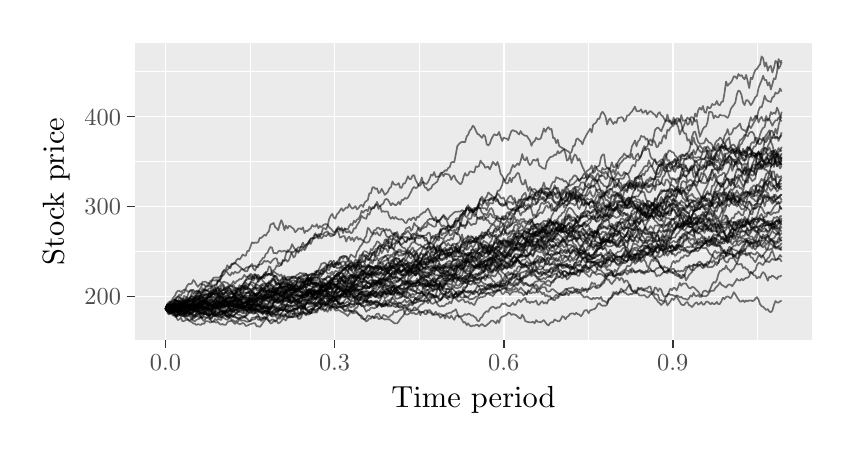
\begin{tikzpicture}[x=1pt,y=1pt]
\definecolor{fillColor}{RGB}{255,255,255}
\path[use as bounding box,fill=fillColor,fill opacity=0.00] (0,0) rectangle (289.08,144.54);
\begin{scope}
\path[clip] (  0.00,  0.00) rectangle (289.08,144.54);
\definecolor{drawColor}{RGB}{255,255,255}
\definecolor{fillColor}{RGB}{255,255,255}

\path[draw=drawColor,line width= 0.6pt,line join=round,line cap=round,fill=fillColor] (  0.00,  0.00) rectangle (289.08,144.54);
\end{scope}
\begin{scope}
\path[clip] ( 38.67, 31.53) rectangle (283.58,139.04);
\definecolor{fillColor}{gray}{0.92}

\path[fill=fillColor] ( 38.67, 31.53) rectangle (283.58,139.04);
\definecolor{drawColor}{RGB}{255,255,255}

\path[draw=drawColor,line width= 0.3pt,line join=round] ( 38.67, 63.63) --
	(283.58, 63.63);

\path[draw=drawColor,line width= 0.3pt,line join=round] ( 38.67, 96.14) --
	(283.58, 96.14);

\path[draw=drawColor,line width= 0.3pt,line join=round] ( 38.67,128.64) --
	(283.58,128.64);

\path[draw=drawColor,line width= 0.3pt,line join=round] ( 80.35, 31.53) --
	( 80.35,139.04);

\path[draw=drawColor,line width= 0.3pt,line join=round] (141.45, 31.53) --
	(141.45,139.04);

\path[draw=drawColor,line width= 0.3pt,line join=round] (202.56, 31.53) --
	(202.56,139.04);

\path[draw=drawColor,line width= 0.3pt,line join=round] (263.66, 31.53) --
	(263.66,139.04);

\path[draw=drawColor,line width= 0.6pt,line join=round] ( 38.67, 47.38) --
	(283.58, 47.38);

\path[draw=drawColor,line width= 0.6pt,line join=round] ( 38.67, 79.89) --
	(283.58, 79.89);

\path[draw=drawColor,line width= 0.6pt,line join=round] ( 38.67,112.39) --
	(283.58,112.39);

\path[draw=drawColor,line width= 0.6pt,line join=round] ( 49.80, 31.53) --
	( 49.80,139.04);

\path[draw=drawColor,line width= 0.6pt,line join=round] (110.90, 31.53) --
	(110.90,139.04);

\path[draw=drawColor,line width= 0.6pt,line join=round] (172.00, 31.53) --
	(172.00,139.04);

\path[draw=drawColor,line width= 0.6pt,line join=round] (233.11, 31.53) --
	(233.11,139.04);
\definecolor{drawColor}{RGB}{0,0,0}

\path[draw=drawColor,draw opacity=0.55,line width= 0.6pt,line join=round] ( 49.80, 42.93) --
	( 50.36, 43.47) --
	( 50.92, 43.63) --
	( 51.47, 44.54) --
	( 52.03, 45.11) --
	( 52.59, 45.02) --
	( 53.15, 44.16) --
	( 53.71, 43.83) --
	( 54.26, 44.69) --
	( 54.82, 45.37) --
	( 55.38, 44.38) --
	( 55.94, 44.67) --
	( 56.50, 44.71) --
	( 57.05, 46.00) --
	( 57.61, 46.13) --
	( 58.17, 46.28) --
	( 58.73, 46.08) --
	( 59.29, 46.33) --
	( 59.84, 46.17) --
	( 60.40, 45.17) --
	( 60.96, 45.77) --
	( 61.52, 45.87) --
	( 62.08, 45.35) --
	( 62.63, 45.85) --
	( 63.19, 45.67) --
	( 63.75, 45.79) --
	( 64.31, 46.05) --
	( 64.87, 45.04) --
	( 65.42, 44.54) --
	( 65.98, 43.70) --
	( 66.54, 43.72) --
	( 67.10, 43.69) --
	( 67.66, 43.95) --
	( 68.21, 44.19) --
	( 68.77, 43.63) --
	( 69.33, 44.05) --
	( 69.89, 43.71) --
	( 70.45, 44.47) --
	( 71.00, 44.05) --
	( 71.56, 44.94) --
	( 72.12, 45.43) --
	( 72.68, 44.90) --
	( 73.24, 44.56) --
	( 73.79, 43.89) --
	( 74.35, 45.00) --
	( 74.91, 44.21) --
	( 75.47, 44.94) --
	( 76.03, 44.03) --
	( 76.58, 43.57) --
	( 77.14, 43.03) --
	( 77.70, 43.24) --
	( 78.26, 43.95) --
	( 78.82, 44.15) --
	( 79.37, 44.29) --
	( 79.93, 46.74) --
	( 80.49, 46.95) --
	( 81.05, 45.90) --
	( 81.61, 44.57) --
	( 82.16, 44.56) --
	( 82.72, 44.40) --
	( 83.28, 46.90) --
	( 83.84, 46.40) --
	( 84.40, 45.99) --
	( 84.95, 46.31) --
	( 85.51, 46.52) --
	( 86.07, 47.00) --
	( 86.63, 46.70) --
	( 87.19, 46.47) --
	( 87.74, 45.83) --
	( 88.30, 46.36) --
	( 88.86, 45.71) --
	( 89.42, 45.47) --
	( 89.98, 45.18) --
	( 90.53, 46.26) --
	( 91.09, 45.64) --
	( 91.65, 44.48) --
	( 92.21, 45.76) --
	( 92.77, 47.26) --
	( 93.32, 46.97) --
	( 93.88, 46.71) --
	( 94.44, 45.36) --
	( 95.00, 45.80) --
	( 95.56, 45.47) --
	( 96.11, 45.59) --
	( 96.67, 45.55) --
	( 97.23, 45.45) --
	( 97.79, 45.10) --
	( 98.35, 45.01) --
	( 98.90, 44.69) --
	( 99.46, 44.85) --
	(100.02, 44.39) --
	(100.58, 44.89) --
	(101.14, 45.18) --
	(101.69, 44.98) --
	(102.25, 44.90) --
	(102.81, 44.88) --
	(103.37, 44.98) --
	(103.93, 45.76) --
	(104.48, 46.88) --
	(105.04, 47.07) --
	(105.60, 47.14) --
	(106.16, 48.07) --
	(106.72, 48.07) --
	(107.27, 47.66) --
	(107.83, 48.70) --
	(108.39, 47.12) --
	(108.95, 46.44) --
	(109.51, 46.33) --
	(110.06, 45.87) --
	(110.62, 46.01) --
	(111.18, 46.43) --
	(111.74, 47.48) --
	(112.30, 47.69) --
	(112.85, 47.30) --
	(113.41, 48.50) --
	(113.97, 48.55) --
	(114.53, 48.31) --
	(115.09, 48.43) --
	(115.65, 49.40) --
	(116.20, 49.87) --
	(116.76, 50.19) --
	(117.32, 50.03) --
	(117.88, 50.91) --
	(118.44, 51.60) --
	(118.99, 52.02) --
	(119.55, 51.49) --
	(120.11, 52.18) --
	(120.67, 51.79) --
	(121.23, 53.14) --
	(121.78, 54.09) --
	(122.34, 54.76) --
	(122.90, 55.26) --
	(123.46, 55.03) --
	(124.02, 55.74) --
	(124.57, 56.71) --
	(125.13, 57.22) --
	(125.69, 58.22) --
	(126.25, 57.56) --
	(126.81, 58.91) --
	(127.36, 59.79) --
	(127.92, 59.15) --
	(128.48, 60.06) --
	(129.04, 60.35) --
	(129.60, 60.49) --
	(130.15, 61.22) --
	(130.71, 58.90) --
	(131.27, 60.31) --
	(131.83, 60.47) --
	(132.39, 61.15) --
	(132.94, 61.25) --
	(133.50, 61.16) --
	(134.06, 61.10) --
	(134.62, 60.02) --
	(135.18, 60.59) --
	(135.73, 59.53) --
	(136.29, 59.17) --
	(136.85, 58.92) --
	(137.41, 57.01) --
	(137.97, 58.20) --
	(138.52, 56.88) --
	(139.08, 58.30) --
	(139.64, 58.92) --
	(140.20, 58.13) --
	(140.76, 58.69) --
	(141.31, 57.32) --
	(141.87, 58.57) --
	(142.43, 58.28) --
	(142.99, 57.50) --
	(143.55, 56.94) --
	(144.10, 57.89) --
	(144.66, 58.11) --
	(145.22, 57.96) --
	(145.78, 56.84) --
	(146.34, 57.73) --
	(146.89, 57.94) --
	(147.45, 57.61) --
	(148.01, 57.91) --
	(148.57, 58.03) --
	(149.13, 57.06) --
	(149.68, 56.82) --
	(150.24, 57.95) --
	(150.80, 57.64) --
	(151.36, 58.40) --
	(151.92, 58.46) --
	(152.47, 58.01) --
	(153.03, 59.25) --
	(153.59, 58.68) --
	(154.15, 59.10) --
	(154.71, 59.53) --
	(155.26, 58.26) --
	(155.82, 58.33) --
	(156.38, 57.35) --
	(156.94, 57.01) --
	(157.50, 57.59) --
	(158.05, 59.01) --
	(158.61, 59.76) --
	(159.17, 60.91) --
	(159.73, 59.96) --
	(160.29, 61.44) --
	(160.84, 61.04) --
	(161.40, 60.40) --
	(161.96, 61.15) --
	(162.52, 60.58) --
	(163.08, 60.86) --
	(163.63, 59.66) --
	(164.19, 59.93) --
	(164.75, 59.94) --
	(165.31, 58.69) --
	(165.87, 58.86) --
	(166.42, 58.43) --
	(166.98, 57.55) --
	(167.54, 55.52) --
	(168.10, 57.14) --
	(168.66, 57.79) --
	(169.21, 58.12) --
	(169.77, 57.24) --
	(170.33, 58.38) --
	(170.89, 59.40) --
	(171.45, 58.74) --
	(172.00, 58.32) --
	(172.56, 59.34) --
	(173.12, 59.25) --
	(173.68, 59.91) --
	(174.24, 60.35) --
	(174.79, 60.31) --
	(175.35, 59.67) --
	(175.91, 59.99) --
	(176.47, 59.59) --
	(177.03, 60.96) --
	(177.58, 60.17) --
	(178.14, 58.95) --
	(178.70, 59.42) --
	(179.26, 58.81) --
	(179.82, 58.08) --
	(180.37, 58.52) --
	(180.93, 58.59) --
	(181.49, 58.57) --
	(182.05, 58.89) --
	(182.61, 58.94) --
	(183.17, 60.80) --
	(183.72, 61.17) --
	(184.28, 62.18) --
	(184.84, 61.60) --
	(185.40, 61.75) --
	(185.96, 61.26) --
	(186.51, 60.79) --
	(187.07, 58.79) --
	(187.63, 59.01) --
	(188.19, 59.67) --
	(188.75, 61.07) --
	(189.30, 60.86) --
	(189.86, 60.94) --
	(190.42, 60.35) --
	(190.98, 61.30) --
	(191.54, 60.56) --
	(192.09, 61.53) --
	(192.65, 62.01) --
	(193.21, 60.19) --
	(193.77, 61.35) --
	(194.33, 62.14) --
	(194.88, 61.43) --
	(195.44, 60.78) --
	(196.00, 59.88) --
	(196.56, 60.90) --
	(197.12, 60.27) --
	(197.67, 60.82) --
	(198.23, 60.73) --
	(198.79, 61.41) --
	(199.35, 61.81) --
	(199.91, 62.20) --
	(200.46, 62.88) --
	(201.02, 62.93) --
	(201.58, 62.14) --
	(202.14, 61.01) --
	(202.70, 60.86) --
	(203.25, 60.70) --
	(203.81, 61.03) --
	(204.37, 62.15) --
	(204.93, 63.29) --
	(205.49, 63.65) --
	(206.04, 64.41) --
	(206.60, 65.05) --
	(207.16, 64.95) --
	(207.72, 64.54) --
	(208.28, 64.73) --
	(208.83, 64.95) --
	(209.39, 63.14) --
	(209.95, 62.85) --
	(210.51, 64.29) --
	(211.07, 63.33) --
	(211.62, 62.80) --
	(212.18, 61.84) --
	(212.74, 61.87) --
	(213.30, 61.60) --
	(213.86, 61.83) --
	(214.41, 61.66) --
	(214.97, 60.78) --
	(215.53, 60.58) --
	(216.09, 60.23) --
	(216.65, 59.95) --
	(217.20, 61.34) --
	(217.76, 61.19) --
	(218.32, 60.18) --
	(218.88, 61.26) --
	(219.44, 59.18) --
	(219.99, 59.72) --
	(220.55, 60.13) --
	(221.11, 60.35) --
	(221.67, 61.11) --
	(222.23, 61.68) --
	(222.78, 62.25) --
	(223.34, 63.11) --
	(223.90, 62.65) --
	(224.46, 63.33) --
	(225.02, 63.17) --
	(225.57, 63.67) --
	(226.13, 63.95) --
	(226.69, 64.60) --
	(227.25, 63.57) --
	(227.81, 62.42) --
	(228.36, 63.89) --
	(228.92, 64.52) --
	(229.48, 64.60) --
	(230.04, 64.01) --
	(230.60, 65.11) --
	(231.15, 64.29) --
	(231.71, 65.44) --
	(232.27, 65.07) --
	(232.83, 66.12) --
	(233.39, 65.13) --
	(233.94, 65.46) --
	(234.50, 66.11) --
	(235.06, 66.05) --
	(235.62, 65.92) --
	(236.18, 65.63) --
	(236.73, 65.26) --
	(237.29, 64.97) --
	(237.85, 64.91) --
	(238.41, 65.39) --
	(238.97, 65.15) --
	(239.52, 65.59) --
	(240.08, 65.18) --
	(240.64, 66.70) --
	(241.20, 66.25) --
	(241.76, 67.04) --
	(242.31, 66.10) --
	(242.87, 66.12) --
	(243.43, 65.60) --
	(243.99, 64.87) --
	(244.55, 64.89) --
	(245.10, 65.00) --
	(245.66, 64.25) --
	(246.22, 63.20) --
	(246.78, 62.53) --
	(247.34, 62.43) --
	(247.89, 61.55) --
	(248.45, 61.02) --
	(249.01, 61.13) --
	(249.57, 62.04) --
	(250.13, 62.51) --
	(250.68, 62.04) --
	(251.24, 62.28) --
	(251.80, 60.43) --
	(252.36, 59.84) --
	(252.92, 59.65) --
	(253.48, 60.97) --
	(254.03, 61.22) --
	(254.59, 61.18) --
	(255.15, 62.47) --
	(255.71, 61.86) --
	(256.27, 61.11) --
	(256.82, 61.34) --
	(257.38, 64.19) --
	(257.94, 64.12) --
	(258.50, 64.84) --
	(259.06, 65.87) --
	(259.61, 67.11) --
	(260.17, 67.60) --
	(260.73, 66.48) --
	(261.29, 66.56) --
	(261.85, 66.59) --
	(262.40, 66.47) --
	(262.96, 67.00) --
	(263.52, 67.16) --
	(264.08, 67.38) --
	(264.64, 67.60) --
	(265.19, 67.77) --
	(265.75, 69.84) --
	(266.31, 68.89) --
	(266.87, 69.66) --
	(267.43, 69.65) --
	(267.98, 67.69) --
	(268.54, 67.75) --
	(269.10, 68.34) --
	(269.66, 68.38) --
	(270.22, 69.32) --
	(270.77, 70.21) --
	(271.33, 70.37) --
	(271.89, 69.56) --
	(272.45, 70.46);

\path[draw=drawColor,draw opacity=0.55,line width= 0.6pt,line join=round] ( 49.80, 42.93) --
	( 50.36, 42.15) --
	( 50.92, 40.96) --
	( 51.47, 41.27) --
	( 52.03, 41.44) --
	( 52.59, 42.16) --
	( 53.15, 41.39) --
	( 53.71, 41.13) --
	( 54.26, 41.76) --
	( 54.82, 40.69) --
	( 55.38, 40.34) --
	( 55.94, 40.30) --
	( 56.50, 40.74) --
	( 57.05, 41.66) --
	( 57.61, 42.71) --
	( 58.17, 44.28) --
	( 58.73, 44.13) --
	( 59.29, 43.96) --
	( 59.84, 44.56) --
	( 60.40, 44.18) --
	( 60.96, 44.49) --
	( 61.52, 43.89) --
	( 62.08, 44.93) --
	( 62.63, 43.85) --
	( 63.19, 44.81) --
	( 63.75, 45.08) --
	( 64.31, 44.40) --
	( 64.87, 44.56) --
	( 65.42, 45.21) --
	( 65.98, 44.88) --
	( 66.54, 44.31) --
	( 67.10, 42.43) --
	( 67.66, 43.58) --
	( 68.21, 43.92) --
	( 68.77, 43.60) --
	( 69.33, 43.73) --
	( 69.89, 43.75) --
	( 70.45, 44.37) --
	( 71.00, 45.12) --
	( 71.56, 46.56) --
	( 72.12, 47.70) --
	( 72.68, 47.52) --
	( 73.24, 48.22) --
	( 73.79, 48.25) --
	( 74.35, 48.18) --
	( 74.91, 48.38) --
	( 75.47, 46.53) --
	( 76.03, 46.90) --
	( 76.58, 46.81) --
	( 77.14, 47.46) --
	( 77.70, 46.90) --
	( 78.26, 47.45) --
	( 78.82, 46.32) --
	( 79.37, 46.47) --
	( 79.93, 47.17) --
	( 80.49, 48.03) --
	( 81.05, 47.70) --
	( 81.61, 48.57) --
	( 82.16, 47.55) --
	( 82.72, 48.46) --
	( 83.28, 49.05) --
	( 83.84, 49.85) --
	( 84.40, 50.63) --
	( 84.95, 50.31) --
	( 85.51, 50.57) --
	( 86.07, 50.15) --
	( 86.63, 50.54) --
	( 87.19, 51.82) --
	( 87.74, 53.10) --
	( 88.30, 53.17) --
	( 88.86, 54.31) --
	( 89.42, 54.89) --
	( 89.98, 54.73) --
	( 90.53, 53.14) --
	( 91.09, 53.24) --
	( 91.65, 53.57) --
	( 92.21, 54.36) --
	( 92.77, 54.96) --
	( 93.32, 53.73) --
	( 93.88, 52.83) --
	( 94.44, 53.23) --
	( 95.00, 53.99) --
	( 95.56, 54.61) --
	( 96.11, 53.98) --
	( 96.67, 54.08) --
	( 97.23, 53.98) --
	( 97.79, 53.77) --
	( 98.35, 54.29) --
	( 98.90, 53.76) --
	( 99.46, 53.82) --
	(100.02, 52.94) --
	(100.58, 53.13) --
	(101.14, 54.21) --
	(101.69, 53.46) --
	(102.25, 52.72) --
	(102.81, 52.38) --
	(103.37, 51.96) --
	(103.93, 52.41) --
	(104.48, 50.79) --
	(105.04, 50.37) --
	(105.60, 50.94) --
	(106.16, 49.89) --
	(106.72, 49.63) --
	(107.27, 49.86) --
	(107.83, 50.05) --
	(108.39, 49.65) --
	(108.95, 49.85) --
	(109.51, 51.64) --
	(110.06, 51.88) --
	(110.62, 51.84) --
	(111.18, 50.88) --
	(111.74, 51.48) --
	(112.30, 52.56) --
	(112.85, 53.91) --
	(113.41, 53.52) --
	(113.97, 54.63) --
	(114.53, 54.93) --
	(115.09, 54.06) --
	(115.65, 53.86) --
	(116.20, 54.37) --
	(116.76, 54.80) --
	(117.32, 54.92) --
	(117.88, 55.66) --
	(118.44, 54.42) --
	(118.99, 53.58) --
	(119.55, 53.93) --
	(120.11, 53.85) --
	(120.67, 54.19) --
	(121.23, 53.53) --
	(121.78, 54.47) --
	(122.34, 54.64) --
	(122.90, 53.83) --
	(123.46, 55.01) --
	(124.02, 55.55) --
	(124.57, 54.30) --
	(125.13, 55.40) --
	(125.69, 56.21) --
	(126.25, 57.05) --
	(126.81, 56.93) --
	(127.36, 57.75) --
	(127.92, 57.08) --
	(128.48, 56.66) --
	(129.04, 57.41) --
	(129.60, 57.17) --
	(130.15, 57.22) --
	(130.71, 58.15) --
	(131.27, 59.08) --
	(131.83, 60.74) --
	(132.39, 59.85) --
	(132.94, 58.79) --
	(133.50, 58.08) --
	(134.06, 57.41) --
	(134.62, 56.41) --
	(135.18, 55.52) --
	(135.73, 55.04) --
	(136.29, 54.24) --
	(136.85, 55.54) --
	(137.41, 56.52) --
	(137.97, 57.99) --
	(138.52, 56.69) --
	(139.08, 56.84) --
	(139.64, 57.55) --
	(140.20, 58.05) --
	(140.76, 58.49) --
	(141.31, 57.65) --
	(141.87, 56.01) --
	(142.43, 56.32) --
	(142.99, 55.79) --
	(143.55, 54.83) --
	(144.10, 54.39) --
	(144.66, 54.41) --
	(145.22, 55.21) --
	(145.78, 55.36) --
	(146.34, 56.09) --
	(146.89, 55.61) --
	(147.45, 54.96) --
	(148.01, 55.29) --
	(148.57, 54.82) --
	(149.13, 55.63) --
	(149.68, 54.38) --
	(150.24, 55.49) --
	(150.80, 55.55) --
	(151.36, 56.91) --
	(151.92, 56.07) --
	(152.47, 55.14) --
	(153.03, 54.81) --
	(153.59, 54.30) --
	(154.15, 54.09) --
	(154.71, 54.01) --
	(155.26, 53.79) --
	(155.82, 54.54) --
	(156.38, 54.96) --
	(156.94, 54.91) --
	(157.50, 56.77) --
	(158.05, 55.89) --
	(158.61, 56.90) --
	(159.17, 56.53) --
	(159.73, 56.68) --
	(160.29, 56.12) --
	(160.84, 57.08) --
	(161.40, 56.92) --
	(161.96, 58.00) --
	(162.52, 58.79) --
	(163.08, 57.93) --
	(163.63, 58.12) --
	(164.19, 57.57) --
	(164.75, 57.85) --
	(165.31, 58.24) --
	(165.87, 58.63) --
	(166.42, 58.76) --
	(166.98, 58.28) --
	(167.54, 58.61) --
	(168.10, 59.55) --
	(168.66, 61.41) --
	(169.21, 61.64) --
	(169.77, 61.19) --
	(170.33, 60.68) --
	(170.89, 60.51) --
	(171.45, 60.39) --
	(172.00, 60.10) --
	(172.56, 61.62) --
	(173.12, 62.52) --
	(173.68, 62.29) --
	(174.24, 64.32) --
	(174.79, 65.55) --
	(175.35, 64.99) --
	(175.91, 64.88) --
	(176.47, 64.93) --
	(177.03, 64.69) --
	(177.58, 64.36) --
	(178.14, 65.23) --
	(178.70, 65.78) --
	(179.26, 66.76) --
	(179.82, 66.38) --
	(180.37, 68.45) --
	(180.93, 67.12) --
	(181.49, 66.86) --
	(182.05, 67.60) --
	(182.61, 66.20) --
	(183.17, 65.51) --
	(183.72, 66.67) --
	(184.28, 68.13) --
	(184.84, 67.14) --
	(185.40, 67.28) --
	(185.96, 68.74) --
	(186.51, 66.43) --
	(187.07, 66.22) --
	(187.63, 66.81) --
	(188.19, 67.71) --
	(188.75, 67.80) --
	(189.30, 67.25) --
	(189.86, 68.09) --
	(190.42, 68.65) --
	(190.98, 69.94) --
	(191.54, 70.49) --
	(192.09, 71.70) --
	(192.65, 71.25) --
	(193.21, 71.93) --
	(193.77, 72.38) --
	(194.33, 72.78) --
	(194.88, 70.42) --
	(195.44, 70.49) --
	(196.00, 70.24) --
	(196.56, 68.64) --
	(197.12, 67.98) --
	(197.67, 68.37) --
	(198.23, 68.78) --
	(198.79, 68.40) --
	(199.35, 68.65) --
	(199.91, 68.14) --
	(200.46, 68.48) --
	(201.02, 68.02) --
	(201.58, 67.55) --
	(202.14, 67.65) --
	(202.70, 66.50) --
	(203.25, 66.29) --
	(203.81, 65.65) --
	(204.37, 65.16) --
	(204.93, 65.72) --
	(205.49, 65.61) --
	(206.04, 65.68) --
	(206.60, 65.05) --
	(207.16, 66.67) --
	(207.72, 66.62) --
	(208.28, 67.12) --
	(208.83, 67.37) --
	(209.39, 68.02) --
	(209.95, 67.06) --
	(210.51, 67.65) --
	(211.07, 67.28) --
	(211.62, 67.10) --
	(212.18, 66.38) --
	(212.74, 65.72) --
	(213.30, 65.89) --
	(213.86, 66.64) --
	(214.41, 68.08) --
	(214.97, 68.05) --
	(215.53, 68.67) --
	(216.09, 69.41) --
	(216.65, 70.50) --
	(217.20, 69.79) --
	(217.76, 68.71) --
	(218.32, 67.34) --
	(218.88, 67.36) --
	(219.44, 68.57) --
	(219.99, 69.48) --
	(220.55, 68.47) --
	(221.11, 68.21) --
	(221.67, 67.76) --
	(222.23, 66.79) --
	(222.78, 66.78) --
	(223.34, 67.67) --
	(223.90, 67.68) --
	(224.46, 67.50) --
	(225.02, 67.67) --
	(225.57, 67.31) --
	(226.13, 68.02) --
	(226.69, 67.67) --
	(227.25, 69.46) --
	(227.81, 71.09) --
	(228.36, 71.27) --
	(228.92, 70.48) --
	(229.48, 71.16) --
	(230.04, 70.95) --
	(230.60, 70.93) --
	(231.15, 71.75) --
	(231.71, 73.59) --
	(232.27, 74.76) --
	(232.83, 75.58) --
	(233.39, 75.32) --
	(233.94, 73.79) --
	(234.50, 72.62) --
	(235.06, 73.36) --
	(235.62, 73.89) --
	(236.18, 73.05) --
	(236.73, 74.37) --
	(237.29, 74.06) --
	(237.85, 74.50) --
	(238.41, 73.56) --
	(238.97, 74.03) --
	(239.52, 73.72) --
	(240.08, 74.60) --
	(240.64, 74.93) --
	(241.20, 76.04) --
	(241.76, 75.55) --
	(242.31, 76.56) --
	(242.87, 76.58) --
	(243.43, 76.99) --
	(243.99, 76.73) --
	(244.55, 76.15) --
	(245.10, 77.00) --
	(245.66, 77.04) --
	(246.22, 77.00) --
	(246.78, 77.46) --
	(247.34, 76.43) --
	(247.89, 76.78) --
	(248.45, 76.08) --
	(249.01, 75.53) --
	(249.57, 75.41) --
	(250.13, 74.35) --
	(250.68, 74.98) --
	(251.24, 76.89) --
	(251.80, 76.60) --
	(252.36, 76.70) --
	(252.92, 75.99) --
	(253.48, 74.17) --
	(254.03, 73.49) --
	(254.59, 73.07) --
	(255.15, 74.09) --
	(255.71, 74.21) --
	(256.27, 73.08) --
	(256.82, 72.34) --
	(257.38, 72.42) --
	(257.94, 72.80) --
	(258.50, 72.49) --
	(259.06, 72.72) --
	(259.61, 74.91) --
	(260.17, 75.39) --
	(260.73, 74.80) --
	(261.29, 74.76) --
	(261.85, 74.84) --
	(262.40, 75.47) --
	(262.96, 75.30) --
	(263.52, 75.26) --
	(264.08, 75.59) --
	(264.64, 75.78) --
	(265.19, 75.18) --
	(265.75, 75.34) --
	(266.31, 76.47) --
	(266.87, 76.17) --
	(267.43, 77.44) --
	(267.98, 77.78) --
	(268.54, 77.83) --
	(269.10, 78.78) --
	(269.66, 79.79) --
	(270.22, 80.44) --
	(270.77, 81.04) --
	(271.33, 81.28) --
	(271.89, 81.07) --
	(272.45, 81.96);

\path[draw=drawColor,draw opacity=0.55,line width= 0.6pt,line join=round] ( 49.80, 42.93) --
	( 50.36, 42.03) --
	( 50.92, 41.19) --
	( 51.47, 41.76) --
	( 52.03, 41.56) --
	( 52.59, 41.84) --
	( 53.15, 41.80) --
	( 53.71, 42.12) --
	( 54.26, 42.80) --
	( 54.82, 43.68) --
	( 55.38, 43.13) --
	( 55.94, 43.31) --
	( 56.50, 43.15) --
	( 57.05, 43.40) --
	( 57.61, 42.96) --
	( 58.17, 42.44) --
	( 58.73, 42.32) --
	( 59.29, 43.32) --
	( 59.84, 43.46) --
	( 60.40, 44.19) --
	( 60.96, 43.44) --
	( 61.52, 44.52) --
	( 62.08, 45.36) --
	( 62.63, 45.60) --
	( 63.19, 45.43) --
	( 63.75, 45.92) --
	( 64.31, 46.00) --
	( 64.87, 46.92) --
	( 65.42, 47.14) --
	( 65.98, 47.41) --
	( 66.54, 48.77) --
	( 67.10, 48.33) --
	( 67.66, 48.39) --
	( 68.21, 48.90) --
	( 68.77, 48.28) --
	( 69.33, 48.92) --
	( 69.89, 49.10) --
	( 70.45, 48.43) --
	( 71.00, 48.20) --
	( 71.56, 49.03) --
	( 72.12, 48.27) --
	( 72.68, 47.55) --
	( 73.24, 46.99) --
	( 73.79, 47.23) --
	( 74.35, 47.27) --
	( 74.91, 47.91) --
	( 75.47, 49.05) --
	( 76.03, 48.51) --
	( 76.58, 48.04) --
	( 77.14, 48.93) --
	( 77.70, 49.19) --
	( 78.26, 50.72) --
	( 78.82, 50.31) --
	( 79.37, 50.55) --
	( 79.93, 50.40) --
	( 80.49, 50.03) --
	( 81.05, 50.06) --
	( 81.61, 50.26) --
	( 82.16, 50.54) --
	( 82.72, 49.70) --
	( 83.28, 49.51) --
	( 83.84, 49.53) --
	( 84.40, 48.12) --
	( 84.95, 49.00) --
	( 85.51, 49.80) --
	( 86.07, 51.02) --
	( 86.63, 51.38) --
	( 87.19, 50.02) --
	( 87.74, 50.65) --
	( 88.30, 49.59) --
	( 88.86, 51.17) --
	( 89.42, 50.57) --
	( 89.98, 50.42) --
	( 90.53, 50.31) --
	( 91.09, 51.09) --
	( 91.65, 50.78) --
	( 92.21, 50.92) --
	( 92.77, 50.93) --
	( 93.32, 51.08) --
	( 93.88, 50.98) --
	( 94.44, 50.21) --
	( 95.00, 49.62) --
	( 95.56, 49.71) --
	( 96.11, 50.97) --
	( 96.67, 50.93) --
	( 97.23, 52.31) --
	( 97.79, 53.08) --
	( 98.35, 52.94) --
	( 98.90, 52.46) --
	( 99.46, 52.42) --
	(100.02, 52.43) --
	(100.58, 53.02) --
	(101.14, 53.22) --
	(101.69, 52.85) --
	(102.25, 53.57) --
	(102.81, 52.07) --
	(103.37, 51.79) --
	(103.93, 52.39) --
	(104.48, 52.01) --
	(105.04, 51.37) --
	(105.60, 51.36) --
	(106.16, 51.00) --
	(106.72, 50.85) --
	(107.27, 50.98) --
	(107.83, 49.91) --
	(108.39, 50.12) --
	(108.95, 51.63) --
	(109.51, 51.47) --
	(110.06, 52.78) --
	(110.62, 54.34) --
	(111.18, 54.51) --
	(111.74, 54.76) --
	(112.30, 55.18) --
	(112.85, 54.53) --
	(113.41, 54.03) --
	(113.97, 54.18) --
	(114.53, 54.64) --
	(115.09, 55.12) --
	(115.65, 55.84) --
	(116.20, 57.69) --
	(116.76, 57.81) --
	(117.32, 58.75) --
	(117.88, 58.41) --
	(118.44, 58.42) --
	(118.99, 58.21) --
	(119.55, 60.62) --
	(120.11, 62.37) --
	(120.67, 62.17) --
	(121.23, 63.48) --
	(121.78, 63.78) --
	(122.34, 63.61) --
	(122.90, 63.13) --
	(123.46, 62.69) --
	(124.02, 63.15) --
	(124.57, 62.31) --
	(125.13, 62.51) --
	(125.69, 64.53) --
	(126.25, 64.77) --
	(126.81, 65.31) --
	(127.36, 65.90) --
	(127.92, 65.62) --
	(128.48, 66.07) --
	(129.04, 66.28) --
	(129.60, 67.56) --
	(130.15, 68.09) --
	(130.71, 66.70) --
	(131.27, 67.07) --
	(131.83, 65.06) --
	(132.39, 64.16) --
	(132.94, 63.90) --
	(133.50, 63.19) --
	(134.06, 62.04) --
	(134.62, 62.37) --
	(135.18, 62.13) --
	(135.73, 62.38) --
	(136.29, 63.09) --
	(136.85, 62.99) --
	(137.41, 62.94) --
	(137.97, 61.69) --
	(138.52, 61.17) --
	(139.08, 62.26) --
	(139.64, 61.53) --
	(140.20, 62.91) --
	(140.76, 64.06) --
	(141.31, 64.47) --
	(141.87, 65.03) --
	(142.43, 65.49) --
	(142.99, 65.39) --
	(143.55, 64.92) --
	(144.10, 64.71) --
	(144.66, 65.52) --
	(145.22, 66.61) --
	(145.78, 68.38) --
	(146.34, 69.30) --
	(146.89, 69.15) --
	(147.45, 69.73) --
	(148.01, 69.70) --
	(148.57, 70.24) --
	(149.13, 71.14) --
	(149.68, 71.77) --
	(150.24, 71.95) --
	(150.80, 71.70) --
	(151.36, 72.46) --
	(151.92, 73.04) --
	(152.47, 72.70) --
	(153.03, 72.55) --
	(153.59, 72.61) --
	(154.15, 74.28) --
	(154.71, 74.89) --
	(155.26, 74.67) --
	(155.82, 74.81) --
	(156.38, 75.21) --
	(156.94, 76.70) --
	(157.50, 78.08) --
	(158.05, 78.36) --
	(158.61, 78.68) --
	(159.17, 78.91) --
	(159.73, 78.32) --
	(160.29, 79.24) --
	(160.84, 77.86) --
	(161.40, 78.85) --
	(161.96, 79.47) --
	(162.52, 79.19) --
	(163.08, 80.89) --
	(163.63, 80.78) --
	(164.19, 80.09) --
	(164.75, 81.54) --
	(165.31, 82.23) --
	(165.87, 80.46) --
	(166.42, 81.38) --
	(166.98, 82.75) --
	(167.54, 82.71) --
	(168.10, 82.93) --
	(168.66, 82.76) --
	(169.21, 83.49) --
	(169.77, 84.65) --
	(170.33, 84.01) --
	(170.89, 83.04) --
	(171.45, 82.81) --
	(172.00, 83.18) --
	(172.56, 81.65) --
	(173.12, 80.26) --
	(173.68, 79.12) --
	(174.24, 78.92) --
	(174.79, 78.90) --
	(175.35, 78.51) --
	(175.91, 78.45) --
	(176.47, 78.89) --
	(177.03, 79.45) --
	(177.58, 79.41) --
	(178.14, 79.54) --
	(178.70, 81.07) --
	(179.26, 79.62) --
	(179.82, 78.66) --
	(180.37, 78.99) --
	(180.93, 79.99) --
	(181.49, 79.95) --
	(182.05, 79.70) --
	(182.61, 80.88) --
	(183.17, 80.56) --
	(183.72, 80.76) --
	(184.28, 81.94) --
	(184.84, 83.14) --
	(185.40, 84.35) --
	(185.96, 86.09) --
	(186.51, 86.42) --
	(187.07, 86.15) --
	(187.63, 86.27) --
	(188.19, 86.22) --
	(188.75, 85.09) --
	(189.30, 84.24) --
	(189.86, 85.23) --
	(190.42, 84.53) --
	(190.98, 84.20) --
	(191.54, 85.13) --
	(192.09, 85.11) --
	(192.65, 83.73) --
	(193.21, 84.71) --
	(193.77, 85.54) --
	(194.33, 85.33) --
	(194.88, 87.05) --
	(195.44, 85.66) --
	(196.00, 84.42) --
	(196.56, 83.52) --
	(197.12, 83.90) --
	(197.67, 84.29) --
	(198.23, 82.69) --
	(198.79, 82.29) --
	(199.35, 83.21) --
	(199.91, 83.72) --
	(200.46, 84.63) --
	(201.02, 85.80) --
	(201.58, 86.63) --
	(202.14, 87.09) --
	(202.70, 86.68) --
	(203.25, 86.37) --
	(203.81, 87.27) --
	(204.37, 86.96) --
	(204.93, 88.03) --
	(205.49, 88.24) --
	(206.04, 89.57) --
	(206.60, 89.71) --
	(207.16, 88.53) --
	(207.72, 88.14) --
	(208.28, 87.33) --
	(208.83, 87.23) --
	(209.39, 86.82) --
	(209.95, 87.26) --
	(210.51, 87.53) --
	(211.07, 88.89) --
	(211.62, 90.02) --
	(212.18, 89.46) --
	(212.74, 89.81) --
	(213.30, 89.92) --
	(213.86, 88.58) --
	(214.41, 88.26) --
	(214.97, 86.96) --
	(215.53, 86.79) --
	(216.09, 87.62) --
	(216.65, 88.48) --
	(217.20, 89.25) --
	(217.76, 86.97) --
	(218.32, 86.12) --
	(218.88, 87.59) --
	(219.44, 87.35) --
	(219.99, 90.02) --
	(220.55, 90.18) --
	(221.11, 91.09) --
	(221.67, 90.78) --
	(222.23, 91.84) --
	(222.78, 91.24) --
	(223.34, 92.72) --
	(223.90, 92.70) --
	(224.46, 94.03) --
	(225.02, 94.51) --
	(225.57, 94.35) --
	(226.13, 95.95) --
	(226.69, 97.06) --
	(227.25, 95.16) --
	(227.81, 94.98) --
	(228.36, 94.60) --
	(228.92, 96.09) --
	(229.48, 95.40) --
	(230.04, 94.51) --
	(230.60, 93.77) --
	(231.15, 94.81) --
	(231.71, 95.69) --
	(232.27, 94.95) --
	(232.83, 95.19) --
	(233.39, 96.51) --
	(233.94, 97.17) --
	(234.50, 94.94) --
	(235.06, 93.68) --
	(235.62, 95.12) --
	(236.18, 95.13) --
	(236.73, 93.29) --
	(237.29, 95.18) --
	(237.85, 94.08) --
	(238.41, 93.34) --
	(238.97, 93.25) --
	(239.52, 93.76) --
	(240.08, 93.08) --
	(240.64, 94.35) --
	(241.20, 91.98) --
	(241.76, 91.15) --
	(242.31, 91.82) --
	(242.87, 95.03) --
	(243.43, 96.67) --
	(243.99, 97.23) --
	(244.55, 97.06) --
	(245.10, 97.90) --
	(245.66, 97.31) --
	(246.22, 97.73) --
	(246.78, 97.03) --
	(247.34,100.44) --
	(247.89,101.40) --
	(248.45,100.32) --
	(249.01,100.47) --
	(249.57,101.20) --
	(250.13,101.33) --
	(250.68,101.53) --
	(251.24,101.13) --
	(251.80,101.96) --
	(252.36,103.63) --
	(252.92,104.22) --
	(253.48,104.88) --
	(254.03,101.22) --
	(254.59,100.95) --
	(255.15, 99.34) --
	(255.71, 98.16) --
	(256.27,100.79) --
	(256.82,102.23) --
	(257.38,103.91) --
	(257.94,104.20) --
	(258.50,104.78) --
	(259.06,105.84) --
	(259.61,105.66) --
	(260.17,105.25) --
	(260.73,106.49) --
	(261.29,106.82) --
	(261.85,106.86) --
	(262.40,106.15) --
	(262.96,104.29) --
	(263.52,102.58) --
	(264.08,104.01) --
	(264.64,105.91) --
	(265.19,107.44) --
	(265.75,108.31) --
	(266.31,108.63) --
	(266.87,111.49) --
	(267.43,111.23) --
	(267.98,111.76) --
	(268.54,114.05) --
	(269.10,113.29) --
	(269.66,113.87) --
	(270.22,113.43) --
	(270.77,115.66) --
	(271.33,114.32) --
	(271.89,112.23) --
	(272.45,111.82);

\path[draw=drawColor,draw opacity=0.55,line width= 0.6pt,line join=round] ( 49.80, 42.93) --
	( 50.36, 42.54) --
	( 50.92, 42.15) --
	( 51.47, 43.15) --
	( 52.03, 43.03) --
	( 52.59, 43.30) --
	( 53.15, 44.10) --
	( 53.71, 43.06) --
	( 54.26, 43.00) --
	( 54.82, 43.11) --
	( 55.38, 42.73) --
	( 55.94, 43.25) --
	( 56.50, 43.80) --
	( 57.05, 43.54) --
	( 57.61, 43.11) --
	( 58.17, 42.65) --
	( 58.73, 42.72) --
	( 59.29, 42.90) --
	( 59.84, 42.96) --
	( 60.40, 42.92) --
	( 60.96, 43.40) --
	( 61.52, 43.04) --
	( 62.08, 42.12) --
	( 62.63, 41.24) --
	( 63.19, 41.64) --
	( 63.75, 41.30) --
	( 64.31, 40.93) --
	( 64.87, 40.98) --
	( 65.42, 40.65) --
	( 65.98, 40.27) --
	( 66.54, 41.70) --
	( 67.10, 41.30) --
	( 67.66, 40.56) --
	( 68.21, 40.69) --
	( 68.77, 40.79) --
	( 69.33, 41.16) --
	( 69.89, 40.82) --
	( 70.45, 41.59) --
	( 71.00, 42.34) --
	( 71.56, 41.90) --
	( 72.12, 41.60) --
	( 72.68, 42.34) --
	( 73.24, 42.67) --
	( 73.79, 44.06) --
	( 74.35, 44.04) --
	( 74.91, 43.39) --
	( 75.47, 43.51) --
	( 76.03, 43.75) --
	( 76.58, 43.30) --
	( 77.14, 44.30) --
	( 77.70, 43.64) --
	( 78.26, 43.21) --
	( 78.82, 42.11) --
	( 79.37, 42.67) --
	( 79.93, 43.01) --
	( 80.49, 42.61) --
	( 81.05, 44.55) --
	( 81.61, 44.79) --
	( 82.16, 45.02) --
	( 82.72, 46.29) --
	( 83.28, 46.91) --
	( 83.84, 46.60) --
	( 84.40, 46.96) --
	( 84.95, 46.13) --
	( 85.51, 46.03) --
	( 86.07, 46.05) --
	( 86.63, 45.72) --
	( 87.19, 45.67) --
	( 87.74, 46.20) --
	( 88.30, 46.96) --
	( 88.86, 46.97) --
	( 89.42, 47.18) --
	( 89.98, 47.71) --
	( 90.53, 46.65) --
	( 91.09, 47.34) --
	( 91.65, 47.65) --
	( 92.21, 48.00) --
	( 92.77, 48.72) --
	( 93.32, 49.52) --
	( 93.88, 50.02) --
	( 94.44, 50.10) --
	( 95.00, 49.68) --
	( 95.56, 49.82) --
	( 96.11, 50.94) --
	( 96.67, 51.04) --
	( 97.23, 51.96) --
	( 97.79, 51.97) --
	( 98.35, 52.23) --
	( 98.90, 52.52) --
	( 99.46, 52.87) --
	(100.02, 51.47) --
	(100.58, 52.24) --
	(101.14, 51.57) --
	(101.69, 51.34) --
	(102.25, 51.87) --
	(102.81, 52.40) --
	(103.37, 52.06) --
	(103.93, 51.02) --
	(104.48, 51.20) --
	(105.04, 51.53) --
	(105.60, 51.55) --
	(106.16, 51.12) --
	(106.72, 50.80) --
	(107.27, 50.27) --
	(107.83, 50.00) --
	(108.39, 49.91) --
	(108.95, 50.14) --
	(109.51, 50.23) --
	(110.06, 51.54) --
	(110.62, 51.74) --
	(111.18, 50.86) --
	(111.74, 50.07) --
	(112.30, 50.52) --
	(112.85, 50.10) --
	(113.41, 50.62) --
	(113.97, 50.27) --
	(114.53, 51.20) --
	(115.09, 50.82) --
	(115.65, 50.46) --
	(116.20, 50.91) --
	(116.76, 52.37) --
	(117.32, 51.50) --
	(117.88, 51.27) --
	(118.44, 51.56) --
	(118.99, 51.87) --
	(119.55, 52.93) --
	(120.11, 53.47) --
	(120.67, 52.22) --
	(121.23, 51.15) --
	(121.78, 51.29) --
	(122.34, 52.26) --
	(122.90, 52.21) --
	(123.46, 51.92) --
	(124.02, 51.51) --
	(124.57, 51.01) --
	(125.13, 51.36) --
	(125.69, 52.17) --
	(126.25, 52.38) --
	(126.81, 53.08) --
	(127.36, 52.53) --
	(127.92, 51.22) --
	(128.48, 51.20) --
	(129.04, 51.74) --
	(129.60, 51.20) --
	(130.15, 51.19) --
	(130.71, 51.06) --
	(131.27, 51.57) --
	(131.83, 52.22) --
	(132.39, 52.08) --
	(132.94, 52.48) --
	(133.50, 52.96) --
	(134.06, 53.20) --
	(134.62, 53.69) --
	(135.18, 54.08) --
	(135.73, 54.26) --
	(136.29, 53.57) --
	(136.85, 52.46) --
	(137.41, 53.07) --
	(137.97, 53.33) --
	(138.52, 54.14) --
	(139.08, 54.82) --
	(139.64, 55.05) --
	(140.20, 55.84) --
	(140.76, 55.72) --
	(141.31, 56.64) --
	(141.87, 58.18) --
	(142.43, 59.51) --
	(142.99, 59.41) --
	(143.55, 61.35) --
	(144.10, 60.70) --
	(144.66, 61.41) --
	(145.22, 61.97) --
	(145.78, 63.29) --
	(146.34, 63.85) --
	(146.89, 64.51) --
	(147.45, 64.10) --
	(148.01, 65.93) --
	(148.57, 65.61) --
	(149.13, 65.70) --
	(149.68, 64.01) --
	(150.24, 63.48) --
	(150.80, 62.74) --
	(151.36, 63.01) --
	(151.92, 63.10) --
	(152.47, 62.16) --
	(153.03, 62.73) --
	(153.59, 64.20) --
	(154.15, 63.80) --
	(154.71, 65.63) --
	(155.26, 66.67) --
	(155.82, 66.81) --
	(156.38, 68.08) --
	(156.94, 69.83) --
	(157.50, 67.46) --
	(158.05, 66.49) --
	(158.61, 67.98) --
	(159.17, 68.97) --
	(159.73, 67.89) --
	(160.29, 68.70) --
	(160.84, 68.99) --
	(161.40, 67.77) --
	(161.96, 67.04) --
	(162.52, 68.57) --
	(163.08, 68.04) --
	(163.63, 67.57) --
	(164.19, 69.63) --
	(164.75, 68.58) --
	(165.31, 69.44) --
	(165.87, 69.84) --
	(166.42, 69.54) --
	(166.98, 68.65) --
	(167.54, 69.55) --
	(168.10, 70.03) --
	(168.66, 71.29) --
	(169.21, 70.71) --
	(169.77, 71.60) --
	(170.33, 71.67) --
	(170.89, 70.26) --
	(171.45, 70.23) --
	(172.00, 69.60) --
	(172.56, 70.87) --
	(173.12, 72.11) --
	(173.68, 73.51) --
	(174.24, 72.72) --
	(174.79, 73.27) --
	(175.35, 74.67) --
	(175.91, 76.19) --
	(176.47, 74.96) --
	(177.03, 75.16) --
	(177.58, 74.30) --
	(178.14, 75.36) --
	(178.70, 75.23) --
	(179.26, 75.46) --
	(179.82, 74.57) --
	(180.37, 74.54) --
	(180.93, 74.21) --
	(181.49, 75.33) --
	(182.05, 74.81) --
	(182.61, 73.49) --
	(183.17, 73.29) --
	(183.72, 73.40) --
	(184.28, 73.70) --
	(184.84, 72.61) --
	(185.40, 73.63) --
	(185.96, 72.16) --
	(186.51, 71.94) --
	(187.07, 72.50) --
	(187.63, 72.99) --
	(188.19, 71.96) --
	(188.75, 72.98) --
	(189.30, 73.74) --
	(189.86, 74.05) --
	(190.42, 73.67) --
	(190.98, 74.34) --
	(191.54, 73.92) --
	(192.09, 73.42) --
	(192.65, 72.91) --
	(193.21, 73.50) --
	(193.77, 73.56) --
	(194.33, 76.15) --
	(194.88, 76.35) --
	(195.44, 77.12) --
	(196.00, 76.76) --
	(196.56, 75.85) --
	(197.12, 75.97) --
	(197.67, 75.94) --
	(198.23, 74.54) --
	(198.79, 74.04) --
	(199.35, 72.82) --
	(199.91, 72.86) --
	(200.46, 72.69) --
	(201.02, 71.26) --
	(201.58, 70.40) --
	(202.14, 70.44) --
	(202.70, 71.71) --
	(203.25, 72.04) --
	(203.81, 71.63) --
	(204.37, 70.53) --
	(204.93, 71.04) --
	(205.49, 70.26) --
	(206.04, 71.28) --
	(206.60, 68.66) --
	(207.16, 66.80) --
	(207.72, 64.30) --
	(208.28, 64.88) --
	(208.83, 66.35) --
	(209.39, 67.52) --
	(209.95, 67.45) --
	(210.51, 66.58) --
	(211.07, 67.31) --
	(211.62, 66.59) --
	(212.18, 67.02) --
	(212.74, 66.74) --
	(213.30, 66.42) --
	(213.86, 67.42) --
	(214.41, 67.66) --
	(214.97, 67.66) --
	(215.53, 66.72) --
	(216.09, 64.85) --
	(216.65, 64.92) --
	(217.20, 64.17) --
	(217.76, 63.68) --
	(218.32, 65.24) --
	(218.88, 66.73) --
	(219.44, 66.30) --
	(219.99, 66.33) --
	(220.55, 65.59) --
	(221.11, 65.48) --
	(221.67, 65.41) --
	(222.23, 66.31) --
	(222.78, 67.09) --
	(223.34, 66.74) --
	(223.90, 66.70) --
	(224.46, 65.05) --
	(225.02, 64.75) --
	(225.57, 64.44) --
	(226.13, 65.49) --
	(226.69, 65.57) --
	(227.25, 64.62) --
	(227.81, 65.90) --
	(228.36, 64.80) --
	(228.92, 64.16) --
	(229.48, 63.80) --
	(230.04, 62.23) --
	(230.60, 63.32) --
	(231.15, 63.72) --
	(231.71, 63.78) --
	(232.27, 64.02) --
	(232.83, 62.63) --
	(233.39, 62.88) --
	(233.94, 62.05) --
	(234.50, 62.61) --
	(235.06, 63.47) --
	(235.62, 63.17) --
	(236.18, 64.12) --
	(236.73, 64.02) --
	(237.29, 64.80) --
	(237.85, 63.90) --
	(238.41, 64.09) --
	(238.97, 63.53) --
	(239.52, 63.78) --
	(240.08, 63.97) --
	(240.64, 64.25) --
	(241.20, 64.52) --
	(241.76, 63.87) --
	(242.31, 63.85) --
	(242.87, 64.52) --
	(243.43, 65.67) --
	(243.99, 65.68) --
	(244.55, 67.46) --
	(245.10, 66.76) --
	(245.66, 65.40) --
	(246.22, 65.56) --
	(246.78, 66.74) --
	(247.34, 66.15) --
	(247.89, 66.97) --
	(248.45, 66.68) --
	(249.01, 69.03) --
	(249.57, 69.90) --
	(250.13, 69.22) --
	(250.68, 68.09) --
	(251.24, 68.32) --
	(251.80, 68.02) --
	(252.36, 67.93) --
	(252.92, 68.86) --
	(253.48, 70.07) --
	(254.03, 71.03) --
	(254.59, 72.03) --
	(255.15, 74.14) --
	(255.71, 74.39) --
	(256.27, 73.83) --
	(256.82, 74.40) --
	(257.38, 74.57) --
	(257.94, 75.40) --
	(258.50, 74.74) --
	(259.06, 75.28) --
	(259.61, 74.20) --
	(260.17, 75.04) --
	(260.73, 76.83) --
	(261.29, 78.23) --
	(261.85, 79.12) --
	(262.40, 79.31) --
	(262.96, 79.10) --
	(263.52, 80.23) --
	(264.08, 81.03) --
	(264.64, 80.66) --
	(265.19, 81.14) --
	(265.75, 83.36) --
	(266.31, 83.16) --
	(266.87, 82.50) --
	(267.43, 83.69) --
	(267.98, 82.54) --
	(268.54, 81.85) --
	(269.10, 80.88) --
	(269.66, 81.88) --
	(270.22, 82.50) --
	(270.77, 82.65) --
	(271.33, 83.47) --
	(271.89, 83.78) --
	(272.45, 84.38);

\path[draw=drawColor,draw opacity=0.55,line width= 0.6pt,line join=round] ( 49.80, 42.93) --
	( 50.36, 43.65) --
	( 50.92, 42.70) --
	( 51.47, 43.08) --
	( 52.03, 42.47) --
	( 52.59, 42.77) --
	( 53.15, 42.58) --
	( 53.71, 42.04) --
	( 54.26, 43.01) --
	( 54.82, 43.09) --
	( 55.38, 42.23) --
	( 55.94, 41.48) --
	( 56.50, 41.56) --
	( 57.05, 41.09) --
	( 57.61, 42.03) --
	( 58.17, 42.84) --
	( 58.73, 43.77) --
	( 59.29, 43.95) --
	( 59.84, 44.53) --
	( 60.40, 44.22) --
	( 60.96, 45.30) --
	( 61.52, 44.91) --
	( 62.08, 44.07) --
	( 62.63, 44.32) --
	( 63.19, 45.26) --
	( 63.75, 44.80) --
	( 64.31, 45.84) --
	( 64.87, 45.86) --
	( 65.42, 45.36) --
	( 65.98, 44.74) --
	( 66.54, 44.94) --
	( 67.10, 44.80) --
	( 67.66, 45.72) --
	( 68.21, 45.72) --
	( 68.77, 45.84) --
	( 69.33, 46.41) --
	( 69.89, 46.52) --
	( 70.45, 46.75) --
	( 71.00, 46.48) --
	( 71.56, 46.57) --
	( 72.12, 46.69) --
	( 72.68, 45.58) --
	( 73.24, 45.85) --
	( 73.79, 45.76) --
	( 74.35, 45.52) --
	( 74.91, 46.43) --
	( 75.47, 47.22) --
	( 76.03, 47.46) --
	( 76.58, 47.45) --
	( 77.14, 47.23) --
	( 77.70, 48.25) --
	( 78.26, 48.92) --
	( 78.82, 48.74) --
	( 79.37, 48.54) --
	( 79.93, 48.87) --
	( 80.49, 47.81) --
	( 81.05, 47.34) --
	( 81.61, 48.06) --
	( 82.16, 48.20) --
	( 82.72, 47.88) --
	( 83.28, 48.00) --
	( 83.84, 48.36) --
	( 84.40, 48.31) --
	( 84.95, 47.52) --
	( 85.51, 47.76) --
	( 86.07, 48.14) --
	( 86.63, 49.60) --
	( 87.19, 48.94) --
	( 87.74, 48.77) --
	( 88.30, 48.99) --
	( 88.86, 49.64) --
	( 89.42, 48.49) --
	( 89.98, 48.83) --
	( 90.53, 48.53) --
	( 91.09, 48.64) --
	( 91.65, 49.16) --
	( 92.21, 48.62) --
	( 92.77, 47.43) --
	( 93.32, 48.19) --
	( 93.88, 48.00) --
	( 94.44, 47.59) --
	( 95.00, 47.71) --
	( 95.56, 48.60) --
	( 96.11, 48.64) --
	( 96.67, 50.13) --
	( 97.23, 49.34) --
	( 97.79, 50.04) --
	( 98.35, 50.41) --
	( 98.90, 50.50) --
	( 99.46, 50.10) --
	(100.02, 49.90) --
	(100.58, 49.36) --
	(101.14, 49.72) --
	(101.69, 49.25) --
	(102.25, 49.91) --
	(102.81, 49.37) --
	(103.37, 48.84) --
	(103.93, 48.71) --
	(104.48, 48.99) --
	(105.04, 48.63) --
	(105.60, 48.69) --
	(106.16, 48.97) --
	(106.72, 49.18) --
	(107.27, 49.66) --
	(107.83, 49.85) --
	(108.39, 50.90) --
	(108.95, 51.10) --
	(109.51, 50.20) --
	(110.06, 50.13) --
	(110.62, 50.86) --
	(111.18, 51.65) --
	(111.74, 51.64) --
	(112.30, 51.65) --
	(112.85, 52.28) --
	(113.41, 52.05) --
	(113.97, 51.47) --
	(114.53, 52.05) --
	(115.09, 53.17) --
	(115.65, 53.01) --
	(116.20, 54.14) --
	(116.76, 53.81) --
	(117.32, 54.72) --
	(117.88, 55.03) --
	(118.44, 54.62) --
	(118.99, 54.56) --
	(119.55, 55.20) --
	(120.11, 55.55) --
	(120.67, 56.58) --
	(121.23, 56.73) --
	(121.78, 56.37) --
	(122.34, 55.52) --
	(122.90, 55.24) --
	(123.46, 55.33) --
	(124.02, 54.94) --
	(124.57, 53.69) --
	(125.13, 53.09) --
	(125.69, 53.23) --
	(126.25, 52.78) --
	(126.81, 53.70) --
	(127.36, 53.59) --
	(127.92, 52.61) --
	(128.48, 52.24) --
	(129.04, 52.59) --
	(129.60, 53.36) --
	(130.15, 53.39) --
	(130.71, 54.89) --
	(131.27, 54.99) --
	(131.83, 55.76) --
	(132.39, 55.72) --
	(132.94, 56.99) --
	(133.50, 56.81) --
	(134.06, 57.45) --
	(134.62, 56.96) --
	(135.18, 56.59) --
	(135.73, 56.78) --
	(136.29, 57.54) --
	(136.85, 57.92) --
	(137.41, 58.55) --
	(137.97, 57.82) --
	(138.52, 57.07) --
	(139.08, 58.18) --
	(139.64, 57.47) --
	(140.20, 56.52) --
	(140.76, 56.50) --
	(141.31, 56.06) --
	(141.87, 55.56) --
	(142.43, 55.70) --
	(142.99, 55.20) --
	(143.55, 55.04) --
	(144.10, 54.67) --
	(144.66, 55.48) --
	(145.22, 55.99) --
	(145.78, 56.60) --
	(146.34, 56.79) --
	(146.89, 56.58) --
	(147.45, 56.90) --
	(148.01, 58.37) --
	(148.57, 57.74) --
	(149.13, 56.85) --
	(149.68, 56.38) --
	(150.24, 57.21) --
	(150.80, 59.21) --
	(151.36, 59.21) --
	(151.92, 58.92) --
	(152.47, 59.36) --
	(153.03, 58.55) --
	(153.59, 60.60) --
	(154.15, 60.99) --
	(154.71, 60.81) --
	(155.26, 60.93) --
	(155.82, 60.45) --
	(156.38, 60.77) --
	(156.94, 60.47) --
	(157.50, 59.59) --
	(158.05, 59.87) --
	(158.61, 61.09) --
	(159.17, 61.68) --
	(159.73, 61.89) --
	(160.29, 61.61) --
	(160.84, 61.76) --
	(161.40, 61.50) --
	(161.96, 61.10) --
	(162.52, 59.94) --
	(163.08, 59.46) --
	(163.63, 57.56) --
	(164.19, 56.86) --
	(164.75, 55.91) --
	(165.31, 57.44) --
	(165.87, 58.79) --
	(166.42, 59.66) --
	(166.98, 59.74) --
	(167.54, 60.90) --
	(168.10, 61.61) --
	(168.66, 63.39) --
	(169.21, 64.70) --
	(169.77, 64.75) --
	(170.33, 65.58) --
	(170.89, 66.61) --
	(171.45, 66.79) --
	(172.00, 66.69) --
	(172.56, 66.87) --
	(173.12, 66.99) --
	(173.68, 67.53) --
	(174.24, 65.26) --
	(174.79, 65.67) --
	(175.35, 65.92) --
	(175.91, 66.46) --
	(176.47, 65.94) --
	(177.03, 67.36) --
	(177.58, 66.79) --
	(178.14, 66.25) --
	(178.70, 65.42) --
	(179.26, 65.77) --
	(179.82, 66.54) --
	(180.37, 67.38) --
	(180.93, 67.71) --
	(181.49, 68.25) --
	(182.05, 67.26) --
	(182.61, 67.19) --
	(183.17, 67.13) --
	(183.72, 67.15) --
	(184.28, 66.98) --
	(184.84, 67.66) --
	(185.40, 68.46) --
	(185.96, 69.86) --
	(186.51, 68.96) --
	(187.07, 70.42) --
	(187.63, 69.54) --
	(188.19, 69.22) --
	(188.75, 69.28) --
	(189.30, 67.90) --
	(189.86, 68.29) --
	(190.42, 68.48) --
	(190.98, 67.73) --
	(191.54, 68.30) --
	(192.09, 67.61) --
	(192.65, 67.17) --
	(193.21, 67.67) --
	(193.77, 67.14) --
	(194.33, 67.12) --
	(194.88, 68.26) --
	(195.44, 67.47) --
	(196.00, 67.57) --
	(196.56, 67.61) --
	(197.12, 68.13) --
	(197.67, 69.74) --
	(198.23, 67.25) --
	(198.79, 68.49) --
	(199.35, 69.73) --
	(199.91, 68.24) --
	(200.46, 67.35) --
	(201.02, 67.05) --
	(201.58, 67.70) --
	(202.14, 68.84) --
	(202.70, 69.54) --
	(203.25, 70.77) --
	(203.81, 70.85) --
	(204.37, 68.78) --
	(204.93, 69.31) --
	(205.49, 69.41) --
	(206.04, 70.79) --
	(206.60, 71.65) --
	(207.16, 71.87) --
	(207.72, 73.18) --
	(208.28, 72.39) --
	(208.83, 72.21) --
	(209.39, 71.98) --
	(209.95, 72.10) --
	(210.51, 71.32) --
	(211.07, 73.74) --
	(211.62, 72.61) --
	(212.18, 71.33) --
	(212.74, 70.82) --
	(213.30, 70.95) --
	(213.86, 70.36) --
	(214.41, 70.53) --
	(214.97, 70.23) --
	(215.53, 69.59) --
	(216.09, 69.15) --
	(216.65, 70.36) --
	(217.20, 71.32) --
	(217.76, 70.57) --
	(218.32, 69.82) --
	(218.88, 68.73) --
	(219.44, 68.48) --
	(219.99, 69.13) --
	(220.55, 70.92) --
	(221.11, 68.88) --
	(221.67, 67.64) --
	(222.23, 67.58) --
	(222.78, 67.58) --
	(223.34, 67.41) --
	(223.90, 66.82) --
	(224.46, 67.95) --
	(225.02, 68.17) --
	(225.57, 68.68) --
	(226.13, 68.40) --
	(226.69, 68.73) --
	(227.25, 69.39) --
	(227.81, 69.56) --
	(228.36, 67.45) --
	(228.92, 67.75) --
	(229.48, 69.18) --
	(230.04, 68.83) --
	(230.60, 68.97) --
	(231.15, 69.52) --
	(231.71, 68.81) --
	(232.27, 71.60) --
	(232.83, 71.22) --
	(233.39, 71.22) --
	(233.94, 71.75) --
	(234.50, 72.52) --
	(235.06, 72.31) --
	(235.62, 72.72) --
	(236.18, 73.13) --
	(236.73, 72.55) --
	(237.29, 72.78) --
	(237.85, 73.88) --
	(238.41, 74.45) --
	(238.97, 72.79) --
	(239.52, 72.52) --
	(240.08, 72.69) --
	(240.64, 73.47) --
	(241.20, 74.21) --
	(241.76, 73.65) --
	(242.31, 74.92) --
	(242.87, 74.24) --
	(243.43, 74.28) --
	(243.99, 74.61) --
	(244.55, 75.71) --
	(245.10, 76.73) --
	(245.66, 74.70) --
	(246.22, 75.96) --
	(246.78, 75.25) --
	(247.34, 75.18) --
	(247.89, 75.09) --
	(248.45, 75.84) --
	(249.01, 74.71) --
	(249.57, 74.79) --
	(250.13, 73.79) --
	(250.68, 74.23) --
	(251.24, 74.93) --
	(251.80, 75.28) --
	(252.36, 76.58) --
	(252.92, 74.61) --
	(253.48, 72.43) --
	(254.03, 73.15) --
	(254.59, 72.35) --
	(255.15, 71.49) --
	(255.71, 73.30) --
	(256.27, 74.57) --
	(256.82, 75.03) --
	(257.38, 73.44) --
	(257.94, 72.56) --
	(258.50, 72.78) --
	(259.06, 72.86) --
	(259.61, 72.94) --
	(260.17, 71.20) --
	(260.73, 71.36) --
	(261.29, 71.28) --
	(261.85, 72.52) --
	(262.40, 72.52) --
	(262.96, 70.83) --
	(263.52, 70.54) --
	(264.08, 71.54) --
	(264.64, 73.11) --
	(265.19, 72.36) --
	(265.75, 73.72) --
	(266.31, 72.76) --
	(266.87, 73.37) --
	(267.43, 73.50) --
	(267.98, 73.91) --
	(268.54, 72.99) --
	(269.10, 74.46) --
	(269.66, 76.00) --
	(270.22, 75.79) --
	(270.77, 76.20) --
	(271.33, 75.73) --
	(271.89, 73.69) --
	(272.45, 73.89);

\path[draw=drawColor,draw opacity=0.55,line width= 0.6pt,line join=round] ( 49.80, 42.93) --
	( 50.36, 44.59) --
	( 50.92, 44.32) --
	( 51.47, 43.98) --
	( 52.03, 43.92) --
	( 52.59, 44.31) --
	( 53.15, 43.82) --
	( 53.71, 43.62) --
	( 54.26, 43.79) --
	( 54.82, 43.44) --
	( 55.38, 43.20) --
	( 55.94, 42.61) --
	( 56.50, 42.35) --
	( 57.05, 42.36) --
	( 57.61, 41.37) --
	( 58.17, 42.41) --
	( 58.73, 42.74) --
	( 59.29, 42.52) --
	( 59.84, 41.52) --
	( 60.40, 42.38) --
	( 60.96, 41.99) --
	( 61.52, 42.21) --
	( 62.08, 40.75) --
	( 62.63, 39.87) --
	( 63.19, 39.97) --
	( 63.75, 41.20) --
	( 64.31, 41.31) --
	( 64.87, 40.56) --
	( 65.42, 40.30) --
	( 65.98, 40.76) --
	( 66.54, 41.11) --
	( 67.10, 40.87) --
	( 67.66, 42.14) --
	( 68.21, 41.62) --
	( 68.77, 41.49) --
	( 69.33, 41.76) --
	( 69.89, 42.17) --
	( 70.45, 41.93) --
	( 71.00, 41.17) --
	( 71.56, 42.12) --
	( 72.12, 42.69) --
	( 72.68, 42.68) --
	( 73.24, 42.23) --
	( 73.79, 42.56) --
	( 74.35, 43.27) --
	( 74.91, 44.03) --
	( 75.47, 43.80) --
	( 76.03, 44.43) --
	( 76.58, 43.43) --
	( 77.14, 43.19) --
	( 77.70, 43.98) --
	( 78.26, 43.82) --
	( 78.82, 43.49) --
	( 79.37, 43.35) --
	( 79.93, 43.52) --
	( 80.49, 43.99) --
	( 81.05, 43.00) --
	( 81.61, 43.75) --
	( 82.16, 43.76) --
	( 82.72, 44.10) --
	( 83.28, 44.30) --
	( 83.84, 43.96) --
	( 84.40, 43.96) --
	( 84.95, 43.11) --
	( 85.51, 42.32) --
	( 86.07, 41.82) --
	( 86.63, 41.10) --
	( 87.19, 41.97) --
	( 87.74, 40.46) --
	( 88.30, 40.44) --
	( 88.86, 41.31) --
	( 89.42, 40.90) --
	( 89.98, 41.04) --
	( 90.53, 40.33) --
	( 91.09, 40.89) --
	( 91.65, 40.48) --
	( 92.21, 40.34) --
	( 92.77, 39.80) --
	( 93.32, 41.08) --
	( 93.88, 41.63) --
	( 94.44, 42.36) --
	( 95.00, 41.75) --
	( 95.56, 42.54) --
	( 96.11, 43.09) --
	( 96.67, 42.97) --
	( 97.23, 42.70) --
	( 97.79, 43.05) --
	( 98.35, 43.38) --
	( 98.90, 42.90) --
	( 99.46, 43.53) --
	(100.02, 44.01) --
	(100.58, 42.71) --
	(101.14, 42.57) --
	(101.69, 42.49) --
	(102.25, 42.77) --
	(102.81, 42.92) --
	(103.37, 42.73) --
	(103.93, 42.61) --
	(104.48, 42.80) --
	(105.04, 43.18) --
	(105.60, 43.21) --
	(106.16, 42.50) --
	(106.72, 42.92) --
	(107.27, 42.02) --
	(107.83, 42.85) --
	(108.39, 43.70) --
	(108.95, 43.34) --
	(109.51, 42.34) --
	(110.06, 43.77) --
	(110.62, 43.67) --
	(111.18, 43.76) --
	(111.74, 43.03) --
	(112.30, 43.92) --
	(112.85, 43.94) --
	(113.41, 43.39) --
	(113.97, 44.04) --
	(114.53, 43.88) --
	(115.09, 44.09) --
	(115.65, 44.40) --
	(116.20, 44.22) --
	(116.76, 45.65) --
	(117.32, 45.75) --
	(117.88, 45.58) --
	(118.44, 46.77) --
	(118.99, 46.68) --
	(119.55, 46.70) --
	(120.11, 47.44) --
	(120.67, 46.68) --
	(121.23, 46.32) --
	(121.78, 45.84) --
	(122.34, 45.14) --
	(122.90, 45.90) --
	(123.46, 44.79) --
	(124.02, 44.27) --
	(124.57, 45.15) --
	(125.13, 44.72) --
	(125.69, 44.37) --
	(126.25, 43.53) --
	(126.81, 44.24) --
	(127.36, 44.29) --
	(127.92, 43.65) --
	(128.48, 43.89) --
	(129.04, 44.77) --
	(129.60, 44.11) --
	(130.15, 44.95) --
	(130.71, 45.71) --
	(131.27, 45.33) --
	(131.83, 44.88) --
	(132.39, 44.55) --
	(132.94, 44.77) --
	(133.50, 44.79) --
	(134.06, 43.56) --
	(134.62, 44.10) --
	(135.18, 43.64) --
	(135.73, 43.77) --
	(136.29, 44.37) --
	(136.85, 44.07) --
	(137.41, 44.38) --
	(137.97, 45.04) --
	(138.52, 45.10) --
	(139.08, 45.29) --
	(139.64, 46.10) --
	(140.20, 46.89) --
	(140.76, 46.05) --
	(141.31, 46.25) --
	(141.87, 45.77) --
	(142.43, 45.78) --
	(142.99, 45.43) --
	(143.55, 46.65) --
	(144.10, 47.11) --
	(144.66, 48.10) --
	(145.22, 49.14) --
	(145.78, 49.63) --
	(146.34, 49.27) --
	(146.89, 49.64) --
	(147.45, 50.31) --
	(148.01, 49.88) --
	(148.57, 50.61) --
	(149.13, 49.17) --
	(149.68, 48.74) --
	(150.24, 48.17) --
	(150.80, 48.60) --
	(151.36, 47.96) --
	(151.92, 47.50) --
	(152.47, 47.37) --
	(153.03, 47.49) --
	(153.59, 47.43) --
	(154.15, 47.91) --
	(154.71, 48.71) --
	(155.26, 49.16) --
	(155.82, 49.40) --
	(156.38, 49.24) --
	(156.94, 48.78) --
	(157.50, 49.55) --
	(158.05, 49.12) --
	(158.61, 49.17) --
	(159.17, 48.67) --
	(159.73, 49.34) --
	(160.29, 48.76) --
	(160.84, 49.03) --
	(161.40, 49.50) --
	(161.96, 49.21) --
	(162.52, 48.88) --
	(163.08, 49.81) --
	(163.63, 49.88) --
	(164.19, 50.20) --
	(164.75, 49.47) --
	(165.31, 50.07) --
	(165.87, 50.89) --
	(166.42, 51.83) --
	(166.98, 50.72) --
	(167.54, 51.62) --
	(168.10, 50.60) --
	(168.66, 51.58) --
	(169.21, 51.78) --
	(169.77, 51.57) --
	(170.33, 50.91) --
	(170.89, 50.91) --
	(171.45, 50.22) --
	(172.00, 50.54) --
	(172.56, 50.09) --
	(173.12, 49.91) --
	(173.68, 50.39) --
	(174.24, 50.09) --
	(174.79, 50.21) --
	(175.35, 50.89) --
	(175.91, 51.66) --
	(176.47, 52.32) --
	(177.03, 51.44) --
	(177.58, 52.18) --
	(178.14, 52.80) --
	(178.70, 53.16) --
	(179.26, 54.28) --
	(179.82, 54.47) --
	(180.37, 54.96) --
	(180.93, 55.59) --
	(181.49, 55.75) --
	(182.05, 54.73) --
	(182.61, 55.36) --
	(183.17, 55.07) --
	(183.72, 54.53) --
	(184.28, 53.65) --
	(184.84, 53.87) --
	(185.40, 53.43) --
	(185.96, 53.76) --
	(186.51, 54.11) --
	(187.07, 53.68) --
	(187.63, 54.48) --
	(188.19, 54.40) --
	(188.75, 55.00) --
	(189.30, 54.27) --
	(189.86, 55.17) --
	(190.42, 55.62) --
	(190.98, 55.62) --
	(191.54, 54.82) --
	(192.09, 54.42) --
	(192.65, 54.39) --
	(193.21, 53.94) --
	(193.77, 54.92) --
	(194.33, 54.89) --
	(194.88, 55.92) --
	(195.44, 55.56) --
	(196.00, 56.71) --
	(196.56, 57.22) --
	(197.12, 58.25) --
	(197.67, 59.55) --
	(198.23, 59.89) --
	(198.79, 61.37) --
	(199.35, 62.76) --
	(199.91, 62.45) --
	(200.46, 61.37) --
	(201.02, 61.32) --
	(201.58, 61.80) --
	(202.14, 61.40) --
	(202.70, 62.50) --
	(203.25, 61.95) --
	(203.81, 61.72) --
	(204.37, 61.18) --
	(204.93, 61.36) --
	(205.49, 62.43) --
	(206.04, 61.91) --
	(206.60, 62.43) --
	(207.16, 62.53) --
	(207.72, 61.56) --
	(208.28, 60.89) --
	(208.83, 59.44) --
	(209.39, 60.67) --
	(209.95, 60.47) --
	(210.51, 61.71) --
	(211.07, 62.07) --
	(211.62, 62.49) --
	(212.18, 62.35) --
	(212.74, 63.16) --
	(213.30, 63.57) --
	(213.86, 63.62) --
	(214.41, 63.81) --
	(214.97, 64.76) --
	(215.53, 65.00) --
	(216.09, 64.29) --
	(216.65, 63.65) --
	(217.20, 62.19) --
	(217.76, 63.64) --
	(218.32, 63.01) --
	(218.88, 64.18) --
	(219.44, 64.44) --
	(219.99, 63.82) --
	(220.55, 64.31) --
	(221.11, 63.62) --
	(221.67, 63.78) --
	(222.23, 62.01) --
	(222.78, 61.06) --
	(223.34, 62.55) --
	(223.90, 62.86) --
	(224.46, 62.38) --
	(225.02, 61.83) --
	(225.57, 62.43) --
	(226.13, 61.25) --
	(226.69, 61.14) --
	(227.25, 62.13) --
	(227.81, 61.74) --
	(228.36, 61.64) --
	(228.92, 62.00) --
	(229.48, 62.59) --
	(230.04, 63.75) --
	(230.60, 63.19) --
	(231.15, 62.11) --
	(231.71, 62.90) --
	(232.27, 63.77) --
	(232.83, 63.92) --
	(233.39, 64.06) --
	(233.94, 64.08) --
	(234.50, 64.23) --
	(235.06, 65.19) --
	(235.62, 64.40) --
	(236.18, 64.45) --
	(236.73, 64.46) --
	(237.29, 63.73) --
	(237.85, 64.28) --
	(238.41, 63.29) --
	(238.97, 63.13) --
	(239.52, 63.32) --
	(240.08, 63.99) --
	(240.64, 63.81) --
	(241.20, 64.52) --
	(241.76, 64.68) --
	(242.31, 65.12) --
	(242.87, 65.09) --
	(243.43, 65.02) --
	(243.99, 66.46) --
	(244.55, 66.55) --
	(245.10, 66.76) --
	(245.66, 66.65) --
	(246.22, 67.14) --
	(246.78, 66.90) --
	(247.34, 68.27) --
	(247.89, 66.58) --
	(248.45, 65.74) --
	(249.01, 65.53) --
	(249.57, 65.62) --
	(250.13, 65.73) --
	(250.68, 65.17) --
	(251.24, 64.03) --
	(251.80, 63.73) --
	(252.36, 63.09) --
	(252.92, 64.22) --
	(253.48, 63.75) --
	(254.03, 64.89) --
	(254.59, 63.25) --
	(255.15, 61.93) --
	(255.71, 61.71) --
	(256.27, 63.06) --
	(256.82, 62.88) --
	(257.38, 63.55) --
	(257.94, 65.00) --
	(258.50, 65.97) --
	(259.06, 66.31) --
	(259.61, 67.43) --
	(260.17, 66.77) --
	(260.73, 66.07) --
	(261.29, 67.17) --
	(261.85, 66.70) --
	(262.40, 67.23) --
	(262.96, 67.62) --
	(263.52, 66.62) --
	(264.08, 67.73) --
	(264.64, 66.83) --
	(265.19, 65.69) --
	(265.75, 66.57) --
	(266.31, 67.13) --
	(266.87, 66.10) --
	(267.43, 66.85) --
	(267.98, 67.07) --
	(268.54, 68.24) --
	(269.10, 67.57) --
	(269.66, 67.48) --
	(270.22, 66.15) --
	(270.77, 66.79) --
	(271.33, 68.61) --
	(271.89, 67.96) --
	(272.45, 67.48);

\path[draw=drawColor,draw opacity=0.55,line width= 0.6pt,line join=round] ( 49.80, 42.93) --
	( 50.36, 43.38) --
	( 50.92, 44.58) --
	( 51.47, 44.37) --
	( 52.03, 44.86) --
	( 52.59, 44.64) --
	( 53.15, 43.64) --
	( 53.71, 42.53) --
	( 54.26, 43.87) --
	( 54.82, 44.09) --
	( 55.38, 43.49) --
	( 55.94, 44.21) --
	( 56.50, 43.67) --
	( 57.05, 42.85) --
	( 57.61, 42.80) --
	( 58.17, 43.99) --
	( 58.73, 44.37) --
	( 59.29, 44.64) --
	( 59.84, 46.22) --
	( 60.40, 45.67) --
	( 60.96, 45.08) --
	( 61.52, 45.31) --
	( 62.08, 44.88) --
	( 62.63, 44.67) --
	( 63.19, 45.81) --
	( 63.75, 46.30) --
	( 64.31, 46.80) --
	( 64.87, 46.86) --
	( 65.42, 47.15) --
	( 65.98, 46.99) --
	( 66.54, 48.58) --
	( 67.10, 49.04) --
	( 67.66, 48.67) --
	( 68.21, 50.16) --
	( 68.77, 50.45) --
	( 69.33, 49.44) --
	( 69.89, 50.95) --
	( 70.45, 51.56) --
	( 71.00, 49.72) --
	( 71.56, 50.18) --
	( 72.12, 51.10) --
	( 72.68, 50.79) --
	( 73.24, 51.19) --
	( 73.79, 51.36) --
	( 74.35, 50.31) --
	( 74.91, 50.48) --
	( 75.47, 50.53) --
	( 76.03, 50.38) --
	( 76.58, 50.34) --
	( 77.14, 49.72) --
	( 77.70, 50.91) --
	( 78.26, 51.25) --
	( 78.82, 51.45) --
	( 79.37, 50.37) --
	( 79.93, 50.28) --
	( 80.49, 49.92) --
	( 81.05, 49.62) --
	( 81.61, 50.57) --
	( 82.16, 50.60) --
	( 82.72, 52.36) --
	( 83.28, 52.83) --
	( 83.84, 54.35) --
	( 84.40, 54.01) --
	( 84.95, 53.00) --
	( 85.51, 52.52) --
	( 86.07, 51.74) --
	( 86.63, 50.97) --
	( 87.19, 51.14) --
	( 87.74, 51.37) --
	( 88.30, 51.70) --
	( 88.86, 50.73) --
	( 89.42, 51.40) --
	( 89.98, 52.03) --
	( 90.53, 52.35) --
	( 91.09, 51.57) --
	( 91.65, 52.63) --
	( 92.21, 51.58) --
	( 92.77, 51.86) --
	( 93.32, 51.94) --
	( 93.88, 51.79) --
	( 94.44, 52.10) --
	( 95.00, 53.00) --
	( 95.56, 52.01) --
	( 96.11, 51.52) --
	( 96.67, 50.25) --
	( 97.23, 49.12) --
	( 97.79, 49.27) --
	( 98.35, 49.77) --
	( 98.90, 48.69) --
	( 99.46, 49.39) --
	(100.02, 49.42) --
	(100.58, 49.67) --
	(101.14, 48.66) --
	(101.69, 48.52) --
	(102.25, 48.89) --
	(102.81, 47.98) --
	(103.37, 48.80) --
	(103.93, 49.06) --
	(104.48, 49.09) --
	(105.04, 49.21) --
	(105.60, 49.50) --
	(106.16, 50.84) --
	(106.72, 50.39) --
	(107.27, 50.65) --
	(107.83, 49.70) --
	(108.39, 48.41) --
	(108.95, 47.98) --
	(109.51, 46.15) --
	(110.06, 46.79) --
	(110.62, 47.20) --
	(111.18, 46.65) --
	(111.74, 45.66) --
	(112.30, 45.40) --
	(112.85, 44.72) --
	(113.41, 44.70) --
	(113.97, 45.21) --
	(114.53, 46.06) --
	(115.09, 46.78) --
	(115.65, 46.73) --
	(116.20, 46.21) --
	(116.76, 45.82) --
	(117.32, 46.81) --
	(117.88, 47.20) --
	(118.44, 47.27) --
	(118.99, 47.11) --
	(119.55, 46.15) --
	(120.11, 46.58) --
	(120.67, 47.24) --
	(121.23, 47.32) --
	(121.78, 47.46) --
	(122.34, 47.47) --
	(122.90, 46.52) --
	(123.46, 47.41) --
	(124.02, 48.34) --
	(124.57, 48.51) --
	(125.13, 48.38) --
	(125.69, 49.24) --
	(126.25, 48.80) --
	(126.81, 48.89) --
	(127.36, 49.44) --
	(127.92, 49.93) --
	(128.48, 50.68) --
	(129.04, 51.83) --
	(129.60, 52.07) --
	(130.15, 51.08) --
	(130.71, 51.39) --
	(131.27, 52.82) --
	(131.83, 52.06) --
	(132.39, 51.40) --
	(132.94, 49.77) --
	(133.50, 50.48) --
	(134.06, 50.65) --
	(134.62, 50.39) --
	(135.18, 50.15) --
	(135.73, 49.79) --
	(136.29, 50.09) --
	(136.85, 50.30) --
	(137.41, 50.33) --
	(137.97, 51.05) --
	(138.52, 51.65) --
	(139.08, 52.34) --
	(139.64, 52.01) --
	(140.20, 52.26) --
	(140.76, 52.96) --
	(141.31, 53.37) --
	(141.87, 53.33) --
	(142.43, 54.00) --
	(142.99, 54.43) --
	(143.55, 53.50) --
	(144.10, 53.38) --
	(144.66, 52.82) --
	(145.22, 51.81) --
	(145.78, 51.25) --
	(146.34, 51.50) --
	(146.89, 51.37) --
	(147.45, 52.17) --
	(148.01, 51.23) --
	(148.57, 51.50) --
	(149.13, 50.42) --
	(149.68, 51.05) --
	(150.24, 51.32) --
	(150.80, 51.76) --
	(151.36, 52.01) --
	(151.92, 51.15) --
	(152.47, 50.70) --
	(153.03, 50.62) --
	(153.59, 51.60) --
	(154.15, 51.11) --
	(154.71, 51.72) --
	(155.26, 51.33) --
	(155.82, 51.33) --
	(156.38, 52.10) --
	(156.94, 52.05) --
	(157.50, 52.00) --
	(158.05, 52.30) --
	(158.61, 53.90) --
	(159.17, 53.93) --
	(159.73, 54.67) --
	(160.29, 54.32) --
	(160.84, 53.95) --
	(161.40, 54.16) --
	(161.96, 53.72) --
	(162.52, 53.21) --
	(163.08, 53.98) --
	(163.63, 54.43) --
	(164.19, 53.99) --
	(164.75, 54.12) --
	(165.31, 55.51) --
	(165.87, 54.95) --
	(166.42, 54.10) --
	(166.98, 54.36) --
	(167.54, 53.94) --
	(168.10, 52.94) --
	(168.66, 52.84) --
	(169.21, 50.88) --
	(169.77, 51.57) --
	(170.33, 51.24) --
	(170.89, 52.53) --
	(171.45, 52.96) --
	(172.00, 53.81) --
	(172.56, 55.31) --
	(173.12, 55.73) --
	(173.68, 56.26) --
	(174.24, 55.33) --
	(174.79, 56.13) --
	(175.35, 55.54) --
	(175.91, 55.16) --
	(176.47, 55.26) --
	(177.03, 55.39) --
	(177.58, 55.83) --
	(178.14, 53.30) --
	(178.70, 54.13) --
	(179.26, 54.86) --
	(179.82, 54.90) --
	(180.37, 56.52) --
	(180.93, 56.01) --
	(181.49, 56.22) --
	(182.05, 55.86) --
	(182.61, 57.64) --
	(183.17, 59.04) --
	(183.72, 59.94) --
	(184.28, 60.14) --
	(184.84, 61.23) --
	(185.40, 60.52) --
	(185.96, 61.33) --
	(186.51, 60.86) --
	(187.07, 60.15) --
	(187.63, 59.16) --
	(188.19, 59.03) --
	(188.75, 58.61) --
	(189.30, 59.19) --
	(189.86, 59.12) --
	(190.42, 58.88) --
	(190.98, 58.49) --
	(191.54, 58.16) --
	(192.09, 58.78) --
	(192.65, 58.52) --
	(193.21, 58.86) --
	(193.77, 58.34) --
	(194.33, 58.62) --
	(194.88, 58.23) --
	(195.44, 57.79) --
	(196.00, 57.70) --
	(196.56, 58.29) --
	(197.12, 57.21) --
	(197.67, 57.87) --
	(198.23, 59.11) --
	(198.79, 58.72) --
	(199.35, 58.99) --
	(199.91, 58.80) --
	(200.46, 57.85) --
	(201.02, 57.70) --
	(201.58, 58.06) --
	(202.14, 57.23) --
	(202.70, 57.74) --
	(203.25, 57.73) --
	(203.81, 58.50) --
	(204.37, 58.75) --
	(204.93, 58.62) --
	(205.49, 59.03) --
	(206.04, 58.86) --
	(206.60, 59.96) --
	(207.16, 60.17) --
	(207.72, 59.14) --
	(208.28, 61.16) --
	(208.83, 60.33) --
	(209.39, 61.64) --
	(209.95, 61.57) --
	(210.51, 61.13) --
	(211.07, 61.55) --
	(211.62, 60.73) --
	(212.18, 60.94) --
	(212.74, 62.35) --
	(213.30, 61.44) --
	(213.86, 61.71) --
	(214.41, 61.71) --
	(214.97, 61.93) --
	(215.53, 61.85) --
	(216.09, 61.46) --
	(216.65, 62.86) --
	(217.20, 61.47) --
	(217.76, 62.12) --
	(218.32, 61.12) --
	(218.88, 61.85) --
	(219.44, 61.53) --
	(219.99, 60.12) --
	(220.55, 60.55) --
	(221.11, 61.40) --
	(221.67, 61.28) --
	(222.23, 61.71) --
	(222.78, 62.72) --
	(223.34, 62.42) --
	(223.90, 62.33) --
	(224.46, 63.02) --
	(225.02, 62.45) --
	(225.57, 62.43) --
	(226.13, 63.13) --
	(226.69, 63.79) --
	(227.25, 64.94) --
	(227.81, 65.08) --
	(228.36, 64.05) --
	(228.92, 64.70) --
	(229.48, 64.06) --
	(230.04, 64.67) --
	(230.60, 65.36) --
	(231.15, 67.13) --
	(231.71, 67.36) --
	(232.27, 66.71) --
	(232.83, 66.98) --
	(233.39, 67.56) --
	(233.94, 67.07) --
	(234.50, 67.06) --
	(235.06, 67.91) --
	(235.62, 68.03) --
	(236.18, 68.99) --
	(236.73, 70.03) --
	(237.29, 69.87) --
	(237.85, 69.63) --
	(238.41, 68.73) --
	(238.97, 67.07) --
	(239.52, 66.54) --
	(240.08, 66.00) --
	(240.64, 65.21) --
	(241.20, 64.85) --
	(241.76, 65.90) --
	(242.31, 66.38) --
	(242.87, 67.04) --
	(243.43, 66.41) --
	(243.99, 67.67) --
	(244.55, 68.11) --
	(245.10, 67.40) --
	(245.66, 66.00) --
	(246.22, 66.19) --
	(246.78, 66.00) --
	(247.34, 66.72) --
	(247.89, 65.75) --
	(248.45, 66.27) --
	(249.01, 65.80) --
	(249.57, 66.84) --
	(250.13, 66.91) --
	(250.68, 66.99) --
	(251.24, 66.49) --
	(251.80, 66.69) --
	(252.36, 69.12) --
	(252.92, 69.57) --
	(253.48, 70.30) --
	(254.03, 71.39) --
	(254.59, 72.00) --
	(255.15, 71.63) --
	(255.71, 71.32) --
	(256.27, 70.73) --
	(256.82, 71.15) --
	(257.38, 70.66) --
	(257.94, 70.78) --
	(258.50, 70.96) --
	(259.06, 70.89) --
	(259.61, 70.41) --
	(260.17, 69.51) --
	(260.73, 69.81) --
	(261.29, 70.47) --
	(261.85, 71.53) --
	(262.40, 72.24) --
	(262.96, 72.82) --
	(263.52, 72.35) --
	(264.08, 72.77) --
	(264.64, 72.69) --
	(265.19, 73.62) --
	(265.75, 73.37) --
	(266.31, 74.42) --
	(266.87, 73.98) --
	(267.43, 74.33) --
	(267.98, 73.70) --
	(268.54, 73.34) --
	(269.10, 72.00) --
	(269.66, 71.61) --
	(270.22, 73.62) --
	(270.77, 72.70) --
	(271.33, 74.11) --
	(271.89, 73.73) --
	(272.45, 75.04);

\path[draw=drawColor,draw opacity=0.55,line width= 0.6pt,line join=round] ( 49.80, 42.93) --
	( 50.36, 43.55) --
	( 50.92, 44.03) --
	( 51.47, 43.67) --
	( 52.03, 43.74) --
	( 52.59, 44.75) --
	( 53.15, 43.80) --
	( 53.71, 43.90) --
	( 54.26, 44.49) --
	( 54.82, 44.47) --
	( 55.38, 45.61) --
	( 55.94, 45.12) --
	( 56.50, 45.11) --
	( 57.05, 45.05) --
	( 57.61, 44.92) --
	( 58.17, 45.83) --
	( 58.73, 47.05) --
	( 59.29, 48.67) --
	( 59.84, 48.32) --
	( 60.40, 48.42) --
	( 60.96, 48.46) --
	( 61.52, 47.93) --
	( 62.08, 49.32) --
	( 62.63, 48.77) --
	( 63.19, 50.40) --
	( 63.75, 49.49) --
	( 64.31, 50.90) --
	( 64.87, 50.90) --
	( 65.42, 51.73) --
	( 65.98, 52.99) --
	( 66.54, 53.27) --
	( 67.10, 53.32) --
	( 67.66, 53.12) --
	( 68.21, 53.41) --
	( 68.77, 52.63) --
	( 69.33, 53.23) --
	( 69.89, 52.32) --
	( 70.45, 52.54) --
	( 71.00, 52.78) --
	( 71.56, 52.46) --
	( 72.12, 52.34) --
	( 72.68, 51.76) --
	( 73.24, 51.56) --
	( 73.79, 51.94) --
	( 74.35, 52.95) --
	( 74.91, 52.08) --
	( 75.47, 52.94) --
	( 76.03, 53.16) --
	( 76.58, 53.72) --
	( 77.14, 53.61) --
	( 77.70, 54.21) --
	( 78.26, 55.22) --
	( 78.82, 54.50) --
	( 79.37, 54.53) --
	( 79.93, 53.99) --
	( 80.49, 55.63) --
	( 81.05, 55.23) --
	( 81.61, 54.12) --
	( 82.16, 53.84) --
	( 82.72, 54.09) --
	( 83.28, 52.69) --
	( 83.84, 53.38) --
	( 84.40, 54.22) --
	( 84.95, 54.90) --
	( 85.51, 55.25) --
	( 86.07, 54.84) --
	( 86.63, 55.06) --
	( 87.19, 55.57) --
	( 87.74, 55.26) --
	( 88.30, 55.45) --
	( 88.86, 56.45) --
	( 89.42, 56.06) --
	( 89.98, 55.56) --
	( 90.53, 55.44) --
	( 91.09, 54.81) --
	( 91.65, 55.36) --
	( 92.21, 53.86) --
	( 92.77, 52.82) --
	( 93.32, 53.68) --
	( 93.88, 53.33) --
	( 94.44, 53.60) --
	( 95.00, 52.61) --
	( 95.56, 53.12) --
	( 96.11, 53.34) --
	( 96.67, 53.03) --
	( 97.23, 52.59) --
	( 97.79, 54.54) --
	( 98.35, 54.08) --
	( 98.90, 54.38) --
	( 99.46, 54.52) --
	(100.02, 55.20) --
	(100.58, 54.95) --
	(101.14, 55.08) --
	(101.69, 55.04) --
	(102.25, 55.41) --
	(102.81, 55.46) --
	(103.37, 55.63) --
	(103.93, 55.33) --
	(104.48, 56.64) --
	(105.04, 56.91) --
	(105.60, 58.00) --
	(106.16, 59.30) --
	(106.72, 59.33) --
	(107.27, 59.67) --
	(107.83, 59.19) --
	(108.39, 57.56) --
	(108.95, 58.41) --
	(109.51, 58.10) --
	(110.06, 58.61) --
	(110.62, 57.96) --
	(111.18, 58.41) --
	(111.74, 57.61) --
	(112.30, 57.73) --
	(112.85, 57.95) --
	(113.41, 57.93) --
	(113.97, 56.86) --
	(114.53, 57.21) --
	(115.09, 58.44) --
	(115.65, 58.04) --
	(116.20, 58.64) --
	(116.76, 58.15) --
	(117.32, 58.72) --
	(117.88, 58.58) --
	(118.44, 59.14) --
	(118.99, 59.81) --
	(119.55, 58.94) --
	(120.11, 57.53) --
	(120.67, 58.42) --
	(121.23, 58.12) --
	(121.78, 59.05) --
	(122.34, 58.47) --
	(122.90, 58.35) --
	(123.46, 58.35) --
	(124.02, 58.40) --
	(124.57, 57.81) --
	(125.13, 57.69) --
	(125.69, 57.30) --
	(126.25, 57.68) --
	(126.81, 57.19) --
	(127.36, 57.42) --
	(127.92, 57.71) --
	(128.48, 57.94) --
	(129.04, 57.77) --
	(129.60, 56.73) --
	(130.15, 55.88) --
	(130.71, 55.60) --
	(131.27, 55.67) --
	(131.83, 56.19) --
	(132.39, 56.70) --
	(132.94, 56.37) --
	(133.50, 56.86) --
	(134.06, 57.24) --
	(134.62, 56.40) --
	(135.18, 56.24) --
	(135.73, 57.23) --
	(136.29, 56.40) --
	(136.85, 56.36) --
	(137.41, 56.59) --
	(137.97, 56.49) --
	(138.52, 56.69) --
	(139.08, 56.80) --
	(139.64, 56.52) --
	(140.20, 57.28) --
	(140.76, 59.43) --
	(141.31, 59.46) --
	(141.87, 60.05) --
	(142.43, 58.71) --
	(142.99, 57.66) --
	(143.55, 57.85) --
	(144.10, 58.89) --
	(144.66, 57.89) --
	(145.22, 58.19) --
	(145.78, 58.70) --
	(146.34, 57.77) --
	(146.89, 57.71) --
	(147.45, 58.64) --
	(148.01, 58.49) --
	(148.57, 58.33) --
	(149.13, 57.46) --
	(149.68, 58.00) --
	(150.24, 57.43) --
	(150.80, 55.54) --
	(151.36, 55.17) --
	(151.92, 54.71) --
	(152.47, 55.19) --
	(153.03, 55.36) --
	(153.59, 55.22) --
	(154.15, 55.01) --
	(154.71, 55.81) --
	(155.26, 54.16) --
	(155.82, 53.44) --
	(156.38, 54.03) --
	(156.94, 53.32) --
	(157.50, 52.61) --
	(158.05, 52.84) --
	(158.61, 52.11) --
	(159.17, 53.39) --
	(159.73, 54.89) --
	(160.29, 55.41) --
	(160.84, 55.24) --
	(161.40, 55.26) --
	(161.96, 55.62) --
	(162.52, 55.54) --
	(163.08, 55.61) --
	(163.63, 55.17) --
	(164.19, 56.05) --
	(164.75, 56.27) --
	(165.31, 56.49) --
	(165.87, 58.64) --
	(166.42, 57.55) --
	(166.98, 57.63) --
	(167.54, 57.13) --
	(168.10, 56.05) --
	(168.66, 57.49) --
	(169.21, 56.87) --
	(169.77, 57.02) --
	(170.33, 55.60) --
	(170.89, 55.25) --
	(171.45, 53.64) --
	(172.00, 52.65) --
	(172.56, 53.36) --
	(173.12, 54.76) --
	(173.68, 55.22) --
	(174.24, 55.34) --
	(174.79, 55.55) --
	(175.35, 55.36) --
	(175.91, 55.78) --
	(176.47, 54.83) --
	(177.03, 54.78) --
	(177.58, 54.51) --
	(178.14, 55.96) --
	(178.70, 56.10) --
	(179.26, 56.28) --
	(179.82, 56.56) --
	(180.37, 56.78) --
	(180.93, 57.00) --
	(181.49, 55.91) --
	(182.05, 57.16) --
	(182.61, 57.06) --
	(183.17, 56.97) --
	(183.72, 56.36) --
	(184.28, 56.31) --
	(184.84, 55.36) --
	(185.40, 55.96) --
	(185.96, 55.04) --
	(186.51, 56.01) --
	(187.07, 55.18) --
	(187.63, 56.01) --
	(188.19, 56.29) --
	(188.75, 57.36) --
	(189.30, 57.96) --
	(189.86, 57.50) --
	(190.42, 58.41) --
	(190.98, 57.69) --
	(191.54, 59.32) --
	(192.09, 59.19) --
	(192.65, 58.49) --
	(193.21, 57.64) --
	(193.77, 57.79) --
	(194.33, 57.89) --
	(194.88, 59.02) --
	(195.44, 58.53) --
	(196.00, 58.91) --
	(196.56, 57.98) --
	(197.12, 57.83) --
	(197.67, 59.46) --
	(198.23, 59.54) --
	(198.79, 59.54) --
	(199.35, 60.29) --
	(199.91, 59.85) --
	(200.46, 60.94) --
	(201.02, 61.21) --
	(201.58, 61.33) --
	(202.14, 59.74) --
	(202.70, 60.03) --
	(203.25, 59.48) --
	(203.81, 59.99) --
	(204.37, 59.72) --
	(204.93, 60.04) --
	(205.49, 59.11) --
	(206.04, 59.94) --
	(206.60, 59.63) --
	(207.16, 60.00) --
	(207.72, 60.44) --
	(208.28, 59.16) --
	(208.83, 58.72) --
	(209.39, 57.98) --
	(209.95, 58.81) --
	(210.51, 58.47) --
	(211.07, 60.02) --
	(211.62, 60.20) --
	(212.18, 61.28) --
	(212.74, 61.38) --
	(213.30, 60.20) --
	(213.86, 60.16) --
	(214.41, 60.88) --
	(214.97, 62.22) --
	(215.53, 62.77) --
	(216.09, 62.07) --
	(216.65, 61.66) --
	(217.20, 61.75) --
	(217.76, 62.66) --
	(218.32, 61.91) --
	(218.88, 62.54) --
	(219.44, 62.41) --
	(219.99, 62.61) --
	(220.55, 64.01) --
	(221.11, 63.95) --
	(221.67, 64.03) --
	(222.23, 63.86) --
	(222.78, 64.19) --
	(223.34, 65.01) --
	(223.90, 64.68) --
	(224.46, 65.66) --
	(225.02, 64.10) --
	(225.57, 64.76) --
	(226.13, 63.49) --
	(226.69, 63.93) --
	(227.25, 63.51) --
	(227.81, 63.31) --
	(228.36, 64.43) --
	(228.92, 64.81) --
	(229.48, 63.67) --
	(230.04, 64.53) --
	(230.60, 64.38) --
	(231.15, 65.77) --
	(231.71, 65.73) --
	(232.27, 64.91) --
	(232.83, 65.78) --
	(233.39, 65.41) --
	(233.94, 64.69) --
	(234.50, 64.47) --
	(235.06, 65.18) --
	(235.62, 67.22) --
	(236.18, 68.99) --
	(236.73, 68.98) --
	(237.29, 70.11) --
	(237.85, 70.94) --
	(238.41, 70.61) --
	(238.97, 70.28) --
	(239.52, 69.70) --
	(240.08, 69.69) --
	(240.64, 68.96) --
	(241.20, 71.04) --
	(241.76, 70.89) --
	(242.31, 70.35) --
	(242.87, 70.24) --
	(243.43, 69.69) --
	(243.99, 69.01) --
	(244.55, 68.87) --
	(245.10, 67.26) --
	(245.66, 67.46) --
	(246.22, 67.01) --
	(246.78, 68.07) --
	(247.34, 67.74) --
	(247.89, 68.50) --
	(248.45, 68.59) --
	(249.01, 68.13) --
	(249.57, 67.87) --
	(250.13, 66.89) --
	(250.68, 68.55) --
	(251.24, 69.08) --
	(251.80, 67.23) --
	(252.36, 67.66) --
	(252.92, 67.82) --
	(253.48, 68.50) --
	(254.03, 69.34) --
	(254.59, 69.19) --
	(255.15, 68.12) --
	(255.71, 68.55) --
	(256.27, 67.42) --
	(256.82, 68.62) --
	(257.38, 68.71) --
	(257.94, 68.16) --
	(258.50, 68.45) --
	(259.06, 68.18) --
	(259.61, 68.17) --
	(260.17, 67.05) --
	(260.73, 66.72) --
	(261.29, 65.46) --
	(261.85, 64.67) --
	(262.40, 66.01) --
	(262.96, 65.61) --
	(263.52, 65.45) --
	(264.08, 65.58) --
	(264.64, 66.04) --
	(265.19, 65.56) --
	(265.75, 65.12) --
	(266.31, 65.91) --
	(266.87, 64.44) --
	(267.43, 64.58) --
	(267.98, 66.55) --
	(268.54, 66.41) --
	(269.10, 65.99) --
	(269.66, 65.54) --
	(270.22, 64.72) --
	(270.77, 64.74) --
	(271.33, 64.70) --
	(271.89, 64.38) --
	(272.45, 65.44);

\path[draw=drawColor,draw opacity=0.55,line width= 0.6pt,line join=round] ( 49.80, 42.93) --
	( 50.36, 44.27) --
	( 50.92, 43.63) --
	( 51.47, 44.15) --
	( 52.03, 43.26) --
	( 52.59, 43.86) --
	( 53.15, 43.20) --
	( 53.71, 43.38) --
	( 54.26, 42.68) --
	( 54.82, 42.89) --
	( 55.38, 42.99) --
	( 55.94, 43.29) --
	( 56.50, 44.20) --
	( 57.05, 44.95) --
	( 57.61, 43.78) --
	( 58.17, 43.83) --
	( 58.73, 44.70) --
	( 59.29, 43.82) --
	( 59.84, 43.01) --
	( 60.40, 43.24) --
	( 60.96, 42.81) --
	( 61.52, 43.07) --
	( 62.08, 44.39) --
	( 62.63, 44.28) --
	( 63.19, 44.46) --
	( 63.75, 43.55) --
	( 64.31, 43.98) --
	( 64.87, 44.10) --
	( 65.42, 43.99) --
	( 65.98, 44.29) --
	( 66.54, 43.53) --
	( 67.10, 44.51) --
	( 67.66, 45.38) --
	( 68.21, 45.03) --
	( 68.77, 47.35) --
	( 69.33, 47.16) --
	( 69.89, 47.36) --
	( 70.45, 47.21) --
	( 71.00, 46.94) --
	( 71.56, 47.62) --
	( 72.12, 47.88) --
	( 72.68, 48.39) --
	( 73.24, 48.06) --
	( 73.79, 49.21) --
	( 74.35, 48.19) --
	( 74.91, 48.59) --
	( 75.47, 47.68) --
	( 76.03, 47.62) --
	( 76.58, 47.66) --
	( 77.14, 47.46) --
	( 77.70, 47.04) --
	( 78.26, 47.54) --
	( 78.82, 48.11) --
	( 79.37, 48.96) --
	( 79.93, 48.51) --
	( 80.49, 49.66) --
	( 81.05, 49.08) --
	( 81.61, 48.65) --
	( 82.16, 48.27) --
	( 82.72, 46.77) --
	( 83.28, 46.86) --
	( 83.84, 47.31) --
	( 84.40, 48.11) --
	( 84.95, 48.16) --
	( 85.51, 48.68) --
	( 86.07, 48.89) --
	( 86.63, 49.73) --
	( 87.19, 50.03) --
	( 87.74, 48.66) --
	( 88.30, 48.75) --
	( 88.86, 49.26) --
	( 89.42, 50.16) --
	( 89.98, 50.68) --
	( 90.53, 49.88) --
	( 91.09, 51.78) --
	( 91.65, 50.52) --
	( 92.21, 50.03) --
	( 92.77, 50.22) --
	( 93.32, 51.51) --
	( 93.88, 50.97) --
	( 94.44, 49.69) --
	( 95.00, 49.42) --
	( 95.56, 50.09) --
	( 96.11, 50.64) --
	( 96.67, 51.63) --
	( 97.23, 52.72) --
	( 97.79, 52.54) --
	( 98.35, 52.72) --
	( 98.90, 53.67) --
	( 99.46, 53.47) --
	(100.02, 53.79) --
	(100.58, 54.12) --
	(101.14, 53.28) --
	(101.69, 53.74) --
	(102.25, 54.23) --
	(102.81, 53.80) --
	(103.37, 54.20) --
	(103.93, 54.48) --
	(104.48, 55.17) --
	(105.04, 55.33) --
	(105.60, 56.08) --
	(106.16, 55.22) --
	(106.72, 55.54) --
	(107.27, 56.32) --
	(107.83, 56.48) --
	(108.39, 55.67) --
	(108.95, 55.65) --
	(109.51, 55.93) --
	(110.06, 56.38) --
	(110.62, 55.66) --
	(111.18, 56.65) --
	(111.74, 56.51) --
	(112.30, 56.04) --
	(112.85, 57.50) --
	(113.41, 58.26) --
	(113.97, 58.05) --
	(114.53, 57.36) --
	(115.09, 57.87) --
	(115.65, 58.51) --
	(116.20, 57.39) --
	(116.76, 56.73) --
	(117.32, 57.05) --
	(117.88, 57.91) --
	(118.44, 57.88) --
	(118.99, 57.09) --
	(119.55, 57.54) --
	(120.11, 57.25) --
	(120.67, 57.05) --
	(121.23, 55.22) --
	(121.78, 52.98) --
	(122.34, 53.05) --
	(122.90, 52.23) --
	(123.46, 53.13) --
	(124.02, 53.36) --
	(124.57, 53.20) --
	(125.13, 52.23) --
	(125.69, 52.15) --
	(126.25, 51.38) --
	(126.81, 51.83) --
	(127.36, 52.36) --
	(127.92, 52.18) --
	(128.48, 51.47) --
	(129.04, 51.57) --
	(129.60, 50.68) --
	(130.15, 49.88) --
	(130.71, 49.07) --
	(131.27, 49.92) --
	(131.83, 51.11) --
	(132.39, 50.50) --
	(132.94, 49.41) --
	(133.50, 48.85) --
	(134.06, 48.65) --
	(134.62, 48.03) --
	(135.18, 48.15) --
	(135.73, 48.87) --
	(136.29, 49.61) --
	(136.85, 50.30) --
	(137.41, 50.65) --
	(137.97, 50.49) --
	(138.52, 50.05) --
	(139.08, 49.37) --
	(139.64, 49.51) --
	(140.20, 48.85) --
	(140.76, 50.15) --
	(141.31, 49.92) --
	(141.87, 49.24) --
	(142.43, 49.10) --
	(142.99, 48.11) --
	(143.55, 47.59) --
	(144.10, 47.62) --
	(144.66, 48.48) --
	(145.22, 48.74) --
	(145.78, 48.21) --
	(146.34, 47.41) --
	(146.89, 47.14) --
	(147.45, 47.06) --
	(148.01, 47.38) --
	(148.57, 46.84) --
	(149.13, 46.38) --
	(149.68, 46.58) --
	(150.24, 47.21) --
	(150.80, 47.30) --
	(151.36, 46.74) --
	(151.92, 47.26) --
	(152.47, 47.10) --
	(153.03, 47.05) --
	(153.59, 46.82) --
	(154.15, 46.97) --
	(154.71, 47.30) --
	(155.26, 47.57) --
	(155.82, 48.01) --
	(156.38, 47.23) --
	(156.94, 47.00) --
	(157.50, 47.01) --
	(158.05, 47.78) --
	(158.61, 47.18) --
	(159.17, 46.92) --
	(159.73, 46.27) --
	(160.29, 46.51) --
	(160.84, 46.49) --
	(161.40, 46.84) --
	(161.96, 47.38) --
	(162.52, 47.29) --
	(163.08, 47.93) --
	(163.63, 48.83) --
	(164.19, 49.63) --
	(164.75, 50.21) --
	(165.31, 50.83) --
	(165.87, 50.11) --
	(166.42, 50.43) --
	(166.98, 50.22) --
	(167.54, 51.35) --
	(168.10, 51.27) --
	(168.66, 50.62) --
	(169.21, 50.54) --
	(169.77, 51.02) --
	(170.33, 51.86) --
	(170.89, 50.90) --
	(171.45, 51.05) --
	(172.00, 52.03) --
	(172.56, 52.17) --
	(173.12, 52.76) --
	(173.68, 52.69) --
	(174.24, 54.09) --
	(174.79, 53.59) --
	(175.35, 55.34) --
	(175.91, 56.86) --
	(176.47, 56.60) --
	(177.03, 58.03) --
	(177.58, 58.38) --
	(178.14, 58.01) --
	(178.70, 57.71) --
	(179.26, 58.44) --
	(179.82, 59.05) --
	(180.37, 58.08) --
	(180.93, 57.37) --
	(181.49, 58.48) --
	(182.05, 58.39) --
	(182.61, 56.52) --
	(183.17, 56.53) --
	(183.72, 56.80) --
	(184.28, 57.47) --
	(184.84, 57.11) --
	(185.40, 57.11) --
	(185.96, 57.54) --
	(186.51, 58.18) --
	(187.07, 59.49) --
	(187.63, 60.86) --
	(188.19, 61.65) --
	(188.75, 60.92) --
	(189.30, 61.70) --
	(189.86, 62.64) --
	(190.42, 62.48) --
	(190.98, 63.60) --
	(191.54, 63.34) --
	(192.09, 63.00) --
	(192.65, 64.72) --
	(193.21, 64.17) --
	(193.77, 63.87) --
	(194.33, 63.01) --
	(194.88, 64.06) --
	(195.44, 63.94) --
	(196.00, 64.77) --
	(196.56, 65.42) --
	(197.12, 65.55) --
	(197.67, 65.37) --
	(198.23, 64.71) --
	(198.79, 64.07) --
	(199.35, 63.72) --
	(199.91, 64.53) --
	(200.46, 65.84) --
	(201.02, 66.53) --
	(201.58, 66.58) --
	(202.14, 66.88) --
	(202.70, 67.73) --
	(203.25, 68.72) --
	(203.81, 68.97) --
	(204.37, 69.80) --
	(204.93, 68.62) --
	(205.49, 69.09) --
	(206.04, 71.77) --
	(206.60, 73.15) --
	(207.16, 73.82) --
	(207.72, 73.67) --
	(208.28, 74.64) --
	(208.83, 75.30) --
	(209.39, 75.04) --
	(209.95, 75.27) --
	(210.51, 76.40) --
	(211.07, 77.53) --
	(211.62, 78.34) --
	(212.18, 78.35) --
	(212.74, 79.65) --
	(213.30, 81.96) --
	(213.86, 81.41) --
	(214.41, 81.78) --
	(214.97, 81.45) --
	(215.53, 81.54) --
	(216.09, 81.93) --
	(216.65, 82.66) --
	(217.20, 81.34) --
	(217.76, 80.80) --
	(218.32, 81.63) --
	(218.88, 81.57) --
	(219.44, 81.92) --
	(219.99, 81.80) --
	(220.55, 81.37) --
	(221.11, 81.37) --
	(221.67, 80.61) --
	(222.23, 81.00) --
	(222.78, 81.09) --
	(223.34, 80.76) --
	(223.90, 79.32) --
	(224.46, 78.53) --
	(225.02, 78.37) --
	(225.57, 78.91) --
	(226.13, 79.35) --
	(226.69, 79.38) --
	(227.25, 80.66) --
	(227.81, 79.74) --
	(228.36, 79.82) --
	(228.92, 81.40) --
	(229.48, 82.43) --
	(230.04, 82.42) --
	(230.60, 83.30) --
	(231.15, 83.85) --
	(231.71, 84.81) --
	(232.27, 84.61) --
	(232.83, 86.22) --
	(233.39, 85.67) --
	(233.94, 85.49) --
	(234.50, 86.17) --
	(235.06, 86.39) --
	(235.62, 85.32) --
	(236.18, 84.78) --
	(236.73, 82.97) --
	(237.29, 82.54) --
	(237.85, 81.70) --
	(238.41, 82.93) --
	(238.97, 83.87) --
	(239.52, 83.87) --
	(240.08, 84.54) --
	(240.64, 83.36) --
	(241.20, 83.00) --
	(241.76, 82.44) --
	(242.31, 82.97) --
	(242.87, 82.50) --
	(243.43, 83.52) --
	(243.99, 82.94) --
	(244.55, 83.08) --
	(245.10, 84.17) --
	(245.66, 84.62) --
	(246.22, 84.49) --
	(246.78, 84.57) --
	(247.34, 83.41) --
	(247.89, 83.21) --
	(248.45, 85.43) --
	(249.01, 85.30) --
	(249.57, 85.43) --
	(250.13, 85.99) --
	(250.68, 87.79) --
	(251.24, 88.16) --
	(251.80, 90.41) --
	(252.36, 91.27) --
	(252.92, 92.03) --
	(253.48, 93.50) --
	(254.03, 95.15) --
	(254.59, 92.78) --
	(255.15, 94.39) --
	(255.71, 95.68) --
	(256.27, 96.13) --
	(256.82, 96.90) --
	(257.38, 96.17) --
	(257.94, 95.11) --
	(258.50, 91.91) --
	(259.06, 94.47) --
	(259.61, 92.24) --
	(260.17, 93.26) --
	(260.73, 93.58) --
	(261.29, 93.26) --
	(261.85, 95.28) --
	(262.40, 96.39) --
	(262.96, 98.92) --
	(263.52, 97.88) --
	(264.08, 99.77) --
	(264.64, 98.58) --
	(265.19, 99.02) --
	(265.75, 95.95) --
	(266.31, 95.12) --
	(266.87, 95.04) --
	(267.43, 96.04) --
	(267.98, 95.78) --
	(268.54, 95.40) --
	(269.10, 94.90) --
	(269.66, 95.08) --
	(270.22, 96.48) --
	(270.77, 98.32) --
	(271.33, 99.65) --
	(271.89, 99.99) --
	(272.45,101.51);

\path[draw=drawColor,draw opacity=0.55,line width= 0.6pt,line join=round] ( 49.80, 42.93) --
	( 50.36, 43.05) --
	( 50.92, 43.23) --
	( 51.47, 42.28) --
	( 52.03, 41.58) --
	( 52.59, 42.46) --
	( 53.15, 42.47) --
	( 53.71, 41.91) --
	( 54.26, 41.63) --
	( 54.82, 41.97) --
	( 55.38, 41.03) --
	( 55.94, 41.39) --
	( 56.50, 41.19) --
	( 57.05, 41.17) --
	( 57.61, 41.67) --
	( 58.17, 41.80) --
	( 58.73, 41.32) --
	( 59.29, 40.15) --
	( 59.84, 39.33) --
	( 60.40, 39.90) --
	( 60.96, 40.18) --
	( 61.52, 40.78) --
	( 62.08, 41.17) --
	( 62.63, 41.64) --
	( 63.19, 42.53) --
	( 63.75, 42.07) --
	( 64.31, 41.99) --
	( 64.87, 42.22) --
	( 65.42, 41.79) --
	( 65.98, 41.02) --
	( 66.54, 41.35) --
	( 67.10, 40.89) --
	( 67.66, 40.98) --
	( 68.21, 40.49) --
	( 68.77, 41.42) --
	( 69.33, 41.58) --
	( 69.89, 40.89) --
	( 70.45, 41.35) --
	( 71.00, 40.76) --
	( 71.56, 41.23) --
	( 72.12, 41.08) --
	( 72.68, 40.92) --
	( 73.24, 40.61) --
	( 73.79, 40.66) --
	( 74.35, 40.25) --
	( 74.91, 40.90) --
	( 75.47, 41.78) --
	( 76.03, 42.10) --
	( 76.58, 41.76) --
	( 77.14, 41.75) --
	( 77.70, 41.24) --
	( 78.26, 42.21) --
	( 78.82, 42.48) --
	( 79.37, 42.62) --
	( 79.93, 42.58) --
	( 80.49, 42.81) --
	( 81.05, 43.82) --
	( 81.61, 44.35) --
	( 82.16, 44.58) --
	( 82.72, 44.05) --
	( 83.28, 44.31) --
	( 83.84, 45.11) --
	( 84.40, 45.80) --
	( 84.95, 46.69) --
	( 85.51, 47.55) --
	( 86.07, 48.56) --
	( 86.63, 48.36) --
	( 87.19, 49.09) --
	( 87.74, 48.79) --
	( 88.30, 48.76) --
	( 88.86, 48.95) --
	( 89.42, 49.33) --
	( 89.98, 49.87) --
	( 90.53, 50.41) --
	( 91.09, 50.70) --
	( 91.65, 50.64) --
	( 92.21, 50.64) --
	( 92.77, 50.24) --
	( 93.32, 49.07) --
	( 93.88, 48.35) --
	( 94.44, 48.22) --
	( 95.00, 47.94) --
	( 95.56, 47.87) --
	( 96.11, 48.64) --
	( 96.67, 49.07) --
	( 97.23, 49.36) --
	( 97.79, 49.05) --
	( 98.35, 49.31) --
	( 98.90, 48.80) --
	( 99.46, 48.70) --
	(100.02, 48.98) --
	(100.58, 48.65) --
	(101.14, 49.06) --
	(101.69, 49.89) --
	(102.25, 48.75) --
	(102.81, 47.99) --
	(103.37, 48.10) --
	(103.93, 48.45) --
	(104.48, 49.27) --
	(105.04, 49.59) --
	(105.60, 48.96) --
	(106.16, 49.21) --
	(106.72, 49.42) --
	(107.27, 49.37) --
	(107.83, 49.55) --
	(108.39, 50.48) --
	(108.95, 50.95) --
	(109.51, 50.99) --
	(110.06, 48.92) --
	(110.62, 48.38) --
	(111.18, 49.23) --
	(111.74, 48.57) --
	(112.30, 47.31) --
	(112.85, 47.71) --
	(113.41, 48.15) --
	(113.97, 48.67) --
	(114.53, 48.81) --
	(115.09, 48.15) --
	(115.65, 46.89) --
	(116.20, 47.48) --
	(116.76, 47.18) --
	(117.32, 47.56) --
	(117.88, 46.86) --
	(118.44, 46.00) --
	(118.99, 46.30) --
	(119.55, 45.21) --
	(120.11, 44.64) --
	(120.67, 44.06) --
	(121.23, 43.98) --
	(121.78, 43.01) --
	(122.34, 41.89) --
	(122.90, 42.44) --
	(123.46, 42.52) --
	(124.02, 43.39) --
	(124.57, 43.35) --
	(125.13, 43.09) --
	(125.69, 43.33) --
	(126.25, 43.79) --
	(126.81, 44.69) --
	(127.36, 44.55) --
	(127.92, 44.16) --
	(128.48, 43.91) --
	(129.04, 44.54) --
	(129.60, 44.47) --
	(130.15, 44.33) --
	(130.71, 44.94) --
	(131.27, 45.89) --
	(131.83, 46.87) --
	(132.39, 46.41) --
	(132.94, 45.68) --
	(133.50, 45.10) --
	(134.06, 44.69) --
	(134.62, 45.08) --
	(135.18, 44.48) --
	(135.73, 44.25) --
	(136.29, 44.01) --
	(136.85, 43.59) --
	(137.41, 42.53) --
	(137.97, 41.92) --
	(138.52, 42.16) --
	(139.08, 42.53) --
	(139.64, 43.53) --
	(140.20, 43.23) --
	(140.76, 42.84) --
	(141.31, 43.60) --
	(141.87, 44.30) --
	(142.43, 44.64) --
	(142.99, 44.87) --
	(143.55, 45.61) --
	(144.10, 45.69) --
	(144.66, 44.97) --
	(145.22, 45.81) --
	(145.78, 46.67) --
	(146.34, 48.01) --
	(146.89, 47.73) --
	(147.45, 47.15) --
	(148.01, 47.61) --
	(148.57, 47.42) --
	(149.13, 48.67) --
	(149.68, 48.17) --
	(150.24, 48.26) --
	(150.80, 48.28) --
	(151.36, 48.76) --
	(151.92, 48.82) --
	(152.47, 49.18) --
	(153.03, 48.50) --
	(153.59, 47.83) --
	(154.15, 46.97) --
	(154.71, 46.61) --
	(155.26, 46.01) --
	(155.82, 45.50) --
	(156.38, 46.00) --
	(156.94, 46.38) --
	(157.50, 46.23) --
	(158.05, 45.26) --
	(158.61, 45.48) --
	(159.17, 45.66) --
	(159.73, 44.76) --
	(160.29, 45.10) --
	(160.84, 44.61) --
	(161.40, 44.31) --
	(161.96, 45.48) --
	(162.52, 46.61) --
	(163.08, 46.82) --
	(163.63, 47.20) --
	(164.19, 47.09) --
	(164.75, 47.38) --
	(165.31, 47.53) --
	(165.87, 48.52) --
	(166.42, 48.67) --
	(166.98, 48.02) --
	(167.54, 47.89) --
	(168.10, 47.50) --
	(168.66, 48.31) --
	(169.21, 49.01) --
	(169.77, 49.99) --
	(170.33, 49.54) --
	(170.89, 49.77) --
	(171.45, 49.93) --
	(172.00, 50.35) --
	(172.56, 50.50) --
	(173.12, 50.46) --
	(173.68, 52.31) --
	(174.24, 52.48) --
	(174.79, 52.01) --
	(175.35, 52.06) --
	(175.91, 52.83) --
	(176.47, 53.63) --
	(177.03, 53.64) --
	(177.58, 53.57) --
	(178.14, 53.88) --
	(178.70, 52.89) --
	(179.26, 52.11) --
	(179.82, 52.34) --
	(180.37, 52.15) --
	(180.93, 51.54) --
	(181.49, 51.16) --
	(182.05, 51.84) --
	(182.61, 51.76) --
	(183.17, 52.53) --
	(183.72, 52.88) --
	(184.28, 52.84) --
	(184.84, 53.66) --
	(185.40, 52.84) --
	(185.96, 52.80) --
	(186.51, 52.89) --
	(187.07, 52.33) --
	(187.63, 52.97) --
	(188.19, 53.20) --
	(188.75, 52.79) --
	(189.30, 52.40) --
	(189.86, 52.44) --
	(190.42, 53.56) --
	(190.98, 54.71) --
	(191.54, 56.25) --
	(192.09, 56.30) --
	(192.65, 55.85) --
	(193.21, 56.22) --
	(193.77, 56.48) --
	(194.33, 56.46) --
	(194.88, 56.06) --
	(195.44, 55.15) --
	(196.00, 55.96) --
	(196.56, 55.43) --
	(197.12, 55.37) --
	(197.67, 56.80) --
	(198.23, 56.48) --
	(198.79, 57.20) --
	(199.35, 56.46) --
	(199.91, 56.57) --
	(200.46, 56.56) --
	(201.02, 58.72) --
	(201.58, 58.46) --
	(202.14, 60.15) --
	(202.70, 61.43) --
	(203.25, 60.89) --
	(203.81, 60.62) --
	(204.37, 61.26) --
	(204.93, 61.31) --
	(205.49, 61.75) --
	(206.04, 62.49) --
	(206.60, 62.35) --
	(207.16, 63.16) --
	(207.72, 62.27) --
	(208.28, 61.51) --
	(208.83, 61.14) --
	(209.39, 60.41) --
	(209.95, 60.91) --
	(210.51, 60.35) --
	(211.07, 59.85) --
	(211.62, 60.65) --
	(212.18, 59.91) --
	(212.74, 59.43) --
	(213.30, 59.15) --
	(213.86, 59.31) --
	(214.41, 60.06) --
	(214.97, 61.29) --
	(215.53, 60.21) --
	(216.09, 60.28) --
	(216.65, 60.09) --
	(217.20, 62.15) --
	(217.76, 61.69) --
	(218.32, 62.71) --
	(218.88, 62.63) --
	(219.44, 62.07) --
	(219.99, 62.78) --
	(220.55, 62.07) --
	(221.11, 63.31) --
	(221.67, 64.34) --
	(222.23, 63.90) --
	(222.78, 64.03) --
	(223.34, 63.16) --
	(223.90, 63.11) --
	(224.46, 62.99) --
	(225.02, 64.05) --
	(225.57, 65.29) --
	(226.13, 63.92) --
	(226.69, 64.88) --
	(227.25, 66.40) --
	(227.81, 66.19) --
	(228.36, 65.66) --
	(228.92, 66.74) --
	(229.48, 68.11) --
	(230.04, 66.66) --
	(230.60, 66.53) --
	(231.15, 67.76) --
	(231.71, 67.64) --
	(232.27, 67.80) --
	(232.83, 69.83) --
	(233.39, 70.28) --
	(233.94, 71.69) --
	(234.50, 72.11) --
	(235.06, 72.74) --
	(235.62, 72.65) --
	(236.18, 72.03) --
	(236.73, 71.70) --
	(237.29, 71.22) --
	(237.85, 71.85) --
	(238.41, 72.96) --
	(238.97, 72.48) --
	(239.52, 72.53) --
	(240.08, 72.45) --
	(240.64, 71.48) --
	(241.20, 70.79) --
	(241.76, 70.38) --
	(242.31, 70.05) --
	(242.87, 70.78) --
	(243.43, 70.88) --
	(243.99, 72.47) --
	(244.55, 73.31) --
	(245.10, 73.39) --
	(245.66, 72.81) --
	(246.22, 71.57) --
	(246.78, 72.40) --
	(247.34, 70.76) --
	(247.89, 71.01) --
	(248.45, 71.13) --
	(249.01, 70.77) --
	(249.57, 71.66) --
	(250.13, 72.22) --
	(250.68, 73.90) --
	(251.24, 74.02) --
	(251.80, 74.20) --
	(252.36, 74.24) --
	(252.92, 74.72) --
	(253.48, 73.89) --
	(254.03, 74.81) --
	(254.59, 74.05) --
	(255.15, 74.34) --
	(255.71, 73.17) --
	(256.27, 73.33) --
	(256.82, 73.74) --
	(257.38, 75.12) --
	(257.94, 74.08) --
	(258.50, 74.13) --
	(259.06, 76.19) --
	(259.61, 75.38) --
	(260.17, 74.25) --
	(260.73, 73.39) --
	(261.29, 74.51) --
	(261.85, 74.97) --
	(262.40, 75.56) --
	(262.96, 75.05) --
	(263.52, 75.80) --
	(264.08, 74.64) --
	(264.64, 75.55) --
	(265.19, 75.26) --
	(265.75, 75.02) --
	(266.31, 73.79) --
	(266.87, 73.99) --
	(267.43, 74.75) --
	(267.98, 74.43) --
	(268.54, 74.55) --
	(269.10, 74.63) --
	(269.66, 72.41) --
	(270.22, 73.26) --
	(270.77, 71.98) --
	(271.33, 71.14) --
	(271.89, 73.04) --
	(272.45, 73.67);

\path[draw=drawColor,draw opacity=0.55,line width= 0.6pt,line join=round] ( 49.80, 42.93) --
	( 50.36, 43.39) --
	( 50.92, 43.67) --
	( 51.47, 43.80) --
	( 52.03, 43.31) --
	( 52.59, 44.37) --
	( 53.15, 46.29) --
	( 53.71, 45.69) --
	( 54.26, 45.76) --
	( 54.82, 44.83) --
	( 55.38, 44.61) --
	( 55.94, 44.16) --
	( 56.50, 43.77) --
	( 57.05, 43.65) --
	( 57.61, 44.55) --
	( 58.17, 44.16) --
	( 58.73, 43.17) --
	( 59.29, 43.73) --
	( 59.84, 43.71) --
	( 60.40, 44.03) --
	( 60.96, 44.00) --
	( 61.52, 43.43) --
	( 62.08, 43.41) --
	( 62.63, 43.32) --
	( 63.19, 43.84) --
	( 63.75, 43.38) --
	( 64.31, 42.88) --
	( 64.87, 43.00) --
	( 65.42, 43.95) --
	( 65.98, 43.62) --
	( 66.54, 43.18) --
	( 67.10, 43.68) --
	( 67.66, 44.45) --
	( 68.21, 45.29) --
	( 68.77, 45.42) --
	( 69.33, 45.05) --
	( 69.89, 44.74) --
	( 70.45, 45.21) --
	( 71.00, 45.35) --
	( 71.56, 45.90) --
	( 72.12, 45.52) --
	( 72.68, 45.15) --
	( 73.24, 45.24) --
	( 73.79, 45.41) --
	( 74.35, 46.23) --
	( 74.91, 46.59) --
	( 75.47, 45.71) --
	( 76.03, 44.50) --
	( 76.58, 44.94) --
	( 77.14, 45.45) --
	( 77.70, 43.23) --
	( 78.26, 43.58) --
	( 78.82, 43.41) --
	( 79.37, 43.34) --
	( 79.93, 43.41) --
	( 80.49, 43.02) --
	( 81.05, 41.95) --
	( 81.61, 42.31) --
	( 82.16, 42.79) --
	( 82.72, 43.07) --
	( 83.28, 42.53) --
	( 83.84, 42.14) --
	( 84.40, 41.83) --
	( 84.95, 41.18) --
	( 85.51, 41.46) --
	( 86.07, 41.04) --
	( 86.63, 41.39) --
	( 87.19, 41.85) --
	( 87.74, 41.08) --
	( 88.30, 41.67) --
	( 88.86, 41.40) --
	( 89.42, 41.82) --
	( 89.98, 41.66) --
	( 90.53, 42.63) --
	( 91.09, 43.05) --
	( 91.65, 43.46) --
	( 92.21, 43.55) --
	( 92.77, 44.19) --
	( 93.32, 43.89) --
	( 93.88, 45.29) --
	( 94.44, 46.42) --
	( 95.00, 45.10) --
	( 95.56, 45.15) --
	( 96.11, 46.00) --
	( 96.67, 46.24) --
	( 97.23, 45.48) --
	( 97.79, 44.86) --
	( 98.35, 45.85) --
	( 98.90, 45.76) --
	( 99.46, 46.06) --
	(100.02, 46.33) --
	(100.58, 46.34) --
	(101.14, 45.70) --
	(101.69, 46.28) --
	(102.25, 46.51) --
	(102.81, 46.47) --
	(103.37, 47.83) --
	(103.93, 48.20) --
	(104.48, 48.94) --
	(105.04, 49.21) --
	(105.60, 49.38) --
	(106.16, 48.10) --
	(106.72, 47.25) --
	(107.27, 46.75) --
	(107.83, 46.66) --
	(108.39, 46.68) --
	(108.95, 46.11) --
	(109.51, 46.43) --
	(110.06, 46.39) --
	(110.62, 47.32) --
	(111.18, 47.06) --
	(111.74, 47.88) --
	(112.30, 47.86) --
	(112.85, 47.13) --
	(113.41, 48.07) --
	(113.97, 47.97) --
	(114.53, 47.41) --
	(115.09, 47.80) --
	(115.65, 48.51) --
	(116.20, 47.97) --
	(116.76, 48.26) --
	(117.32, 47.90) --
	(117.88, 47.20) --
	(118.44, 47.05) --
	(118.99, 47.72) --
	(119.55, 47.76) --
	(120.11, 48.91) --
	(120.67, 49.19) --
	(121.23, 48.74) --
	(121.78, 48.23) --
	(122.34, 47.87) --
	(122.90, 47.63) --
	(123.46, 49.05) --
	(124.02, 48.83) --
	(124.57, 48.42) --
	(125.13, 48.88) --
	(125.69, 48.12) --
	(126.25, 47.30) --
	(126.81, 47.59) --
	(127.36, 47.36) --
	(127.92, 48.03) --
	(128.48, 48.72) --
	(129.04, 48.05) --
	(129.60, 48.34) --
	(130.15, 48.60) --
	(130.71, 48.50) --
	(131.27, 49.67) --
	(131.83, 51.05) --
	(132.39, 51.04) --
	(132.94, 51.56) --
	(133.50, 50.67) --
	(134.06, 51.17) --
	(134.62, 51.14) --
	(135.18, 51.40) --
	(135.73, 51.61) --
	(136.29, 52.17) --
	(136.85, 52.57) --
	(137.41, 52.80) --
	(137.97, 51.91) --
	(138.52, 51.87) --
	(139.08, 52.20) --
	(139.64, 52.33) --
	(140.20, 51.93) --
	(140.76, 52.52) --
	(141.31, 52.72) --
	(141.87, 51.28) --
	(142.43, 51.76) --
	(142.99, 52.01) --
	(143.55, 51.59) --
	(144.10, 51.59) --
	(144.66, 51.07) --
	(145.22, 51.37) --
	(145.78, 52.53) --
	(146.34, 51.17) --
	(146.89, 51.25) --
	(147.45, 51.25) --
	(148.01, 51.87) --
	(148.57, 50.63) --
	(149.13, 49.35) --
	(149.68, 49.57) --
	(150.24, 51.00) --
	(150.80, 52.00) --
	(151.36, 52.03) --
	(151.92, 52.23) --
	(152.47, 51.84) --
	(153.03, 51.61) --
	(153.59, 52.76) --
	(154.15, 54.07) --
	(154.71, 54.10) --
	(155.26, 53.83) --
	(155.82, 54.28) --
	(156.38, 54.73) --
	(156.94, 54.13) --
	(157.50, 53.41) --
	(158.05, 54.60) --
	(158.61, 54.94) --
	(159.17, 54.81) --
	(159.73, 54.69) --
	(160.29, 56.00) --
	(160.84, 56.40) --
	(161.40, 57.95) --
	(161.96, 58.06) --
	(162.52, 58.27) --
	(163.08, 58.36) --
	(163.63, 58.97) --
	(164.19, 59.18) --
	(164.75, 57.93) --
	(165.31, 58.48) --
	(165.87, 59.11) --
	(166.42, 61.13) --
	(166.98, 61.58) --
	(167.54, 60.49) --
	(168.10, 60.16) --
	(168.66, 59.65) --
	(169.21, 59.63) --
	(169.77, 59.29) --
	(170.33, 59.98) --
	(170.89, 60.12) --
	(171.45, 60.58) --
	(172.00, 60.40) --
	(172.56, 60.26) --
	(173.12, 59.51) --
	(173.68, 59.25) --
	(174.24, 58.86) --
	(174.79, 58.26) --
	(175.35, 59.02) --
	(175.91, 60.53) --
	(176.47, 60.42) --
	(177.03, 61.52) --
	(177.58, 61.41) --
	(178.14, 61.66) --
	(178.70, 62.63) --
	(179.26, 64.19) --
	(179.82, 64.26) --
	(180.37, 63.77) --
	(180.93, 62.75) --
	(181.49, 63.15) --
	(182.05, 62.38) --
	(182.61, 61.79) --
	(183.17, 64.00) --
	(183.72, 63.82) --
	(184.28, 63.69) --
	(184.84, 63.45) --
	(185.40, 63.33) --
	(185.96, 63.96) --
	(186.51, 62.31) --
	(187.07, 63.52) --
	(187.63, 62.38) --
	(188.19, 63.34) --
	(188.75, 65.00) --
	(189.30, 64.73) --
	(189.86, 65.89) --
	(190.42, 65.60) --
	(190.98, 66.11) --
	(191.54, 65.68) --
	(192.09, 65.81) --
	(192.65, 67.31) --
	(193.21, 66.80) --
	(193.77, 68.09) --
	(194.33, 67.19) --
	(194.88, 65.68) --
	(195.44, 63.76) --
	(196.00, 62.97) --
	(196.56, 64.16) --
	(197.12, 64.03) --
	(197.67, 63.18) --
	(198.23, 62.44) --
	(198.79, 62.19) --
	(199.35, 64.01) --
	(199.91, 65.90) --
	(200.46, 66.24) --
	(201.02, 67.31) --
	(201.58, 67.36) --
	(202.14, 66.48) --
	(202.70, 65.60) --
	(203.25, 65.82) --
	(203.81, 65.40) --
	(204.37, 64.27) --
	(204.93, 65.52) --
	(205.49, 66.42) --
	(206.04, 66.93) --
	(206.60, 66.48) --
	(207.16, 66.67) --
	(207.72, 66.47) --
	(208.28, 67.39) --
	(208.83, 67.45) --
	(209.39, 68.01) --
	(209.95, 67.45) --
	(210.51, 66.84) --
	(211.07, 67.25) --
	(211.62, 68.00) --
	(212.18, 67.77) --
	(212.74, 67.35) --
	(213.30, 67.87) --
	(213.86, 68.82) --
	(214.41, 68.42) --
	(214.97, 67.52) --
	(215.53, 67.85) --
	(216.09, 67.80) --
	(216.65, 66.80) --
	(217.20, 68.29) --
	(217.76, 69.25) --
	(218.32, 69.30) --
	(218.88, 71.28) --
	(219.44, 71.50) --
	(219.99, 71.64) --
	(220.55, 71.42) --
	(221.11, 72.20) --
	(221.67, 71.40) --
	(222.23, 70.91) --
	(222.78, 71.91) --
	(223.34, 72.47) --
	(223.90, 71.05) --
	(224.46, 70.94) --
	(225.02, 70.09) --
	(225.57, 69.15) --
	(226.13, 66.99) --
	(226.69, 67.25) --
	(227.25, 67.28) --
	(227.81, 67.47) --
	(228.36, 68.44) --
	(228.92, 68.64) --
	(229.48, 69.99) --
	(230.04, 68.34) --
	(230.60, 69.73) --
	(231.15, 70.59) --
	(231.71, 71.90) --
	(232.27, 72.19) --
	(232.83, 72.90) --
	(233.39, 73.60) --
	(233.94, 74.14) --
	(234.50, 74.55) --
	(235.06, 72.91) --
	(235.62, 72.29) --
	(236.18, 73.09) --
	(236.73, 72.02) --
	(237.29, 74.18) --
	(237.85, 75.10) --
	(238.41, 74.74) --
	(238.97, 76.14) --
	(239.52, 75.98) --
	(240.08, 76.88) --
	(240.64, 77.29) --
	(241.20, 77.29) --
	(241.76, 76.14) --
	(242.31, 75.68) --
	(242.87, 75.65) --
	(243.43, 75.72) --
	(243.99, 75.27) --
	(244.55, 74.04) --
	(245.10, 72.79) --
	(245.66, 71.98) --
	(246.22, 73.00) --
	(246.78, 73.23) --
	(247.34, 73.11) --
	(247.89, 72.59) --
	(248.45, 73.47) --
	(249.01, 73.42) --
	(249.57, 73.22) --
	(250.13, 72.06) --
	(250.68, 72.05) --
	(251.24, 72.64) --
	(251.80, 72.13) --
	(252.36, 72.36) --
	(252.92, 74.32) --
	(253.48, 73.73) --
	(254.03, 72.82) --
	(254.59, 72.47) --
	(255.15, 71.47) --
	(255.71, 71.35) --
	(256.27, 71.76) --
	(256.82, 73.54) --
	(257.38, 73.07) --
	(257.94, 72.73) --
	(258.50, 74.45) --
	(259.06, 74.51) --
	(259.61, 74.08) --
	(260.17, 74.19) --
	(260.73, 74.06) --
	(261.29, 72.33) --
	(261.85, 72.21) --
	(262.40, 72.24) --
	(262.96, 72.12) --
	(263.52, 72.82) --
	(264.08, 71.61) --
	(264.64, 71.49) --
	(265.19, 71.96) --
	(265.75, 72.88) --
	(266.31, 73.00) --
	(266.87, 73.07) --
	(267.43, 73.26) --
	(267.98, 73.05) --
	(268.54, 73.78) --
	(269.10, 72.92) --
	(269.66, 74.22) --
	(270.22, 74.56) --
	(270.77, 74.66) --
	(271.33, 74.98) --
	(271.89, 74.48) --
	(272.45, 74.24);

\path[draw=drawColor,draw opacity=0.55,line width= 0.6pt,line join=round] ( 49.80, 42.93) --
	( 50.36, 44.08) --
	( 50.92, 43.70) --
	( 51.47, 43.33) --
	( 52.03, 42.78) --
	( 52.59, 43.81) --
	( 53.15, 44.21) --
	( 53.71, 44.28) --
	( 54.26, 43.87) --
	( 54.82, 44.07) --
	( 55.38, 44.34) --
	( 55.94, 44.99) --
	( 56.50, 45.98) --
	( 57.05, 46.00) --
	( 57.61, 47.10) --
	( 58.17, 48.87) --
	( 58.73, 49.35) --
	( 59.29, 49.41) --
	( 59.84, 49.83) --
	( 60.40, 49.12) --
	( 60.96, 49.42) --
	( 61.52, 48.55) --
	( 62.08, 49.85) --
	( 62.63, 50.71) --
	( 63.19, 52.71) --
	( 63.75, 52.67) --
	( 64.31, 52.78) --
	( 64.87, 52.25) --
	( 65.42, 52.32) --
	( 65.98, 51.63) --
	( 66.54, 52.96) --
	( 67.10, 54.17) --
	( 67.66, 54.22) --
	( 68.21, 54.31) --
	( 68.77, 54.15) --
	( 69.33, 54.39) --
	( 69.89, 54.79) --
	( 70.45, 54.83) --
	( 71.00, 55.47) --
	( 71.56, 56.43) --
	( 72.12, 56.19) --
	( 72.68, 55.33) --
	( 73.24, 54.97) --
	( 73.79, 56.11) --
	( 74.35, 55.55) --
	( 74.91, 56.37) --
	( 75.47, 55.97) --
	( 76.03, 55.99) --
	( 76.58, 56.37) --
	( 77.14, 57.17) --
	( 77.70, 57.25) --
	( 78.26, 56.69) --
	( 78.82, 56.50) --
	( 79.37, 56.52) --
	( 79.93, 58.11) --
	( 80.49, 58.38) --
	( 81.05, 58.38) --
	( 81.61, 57.32) --
	( 82.16, 56.80) --
	( 82.72, 58.06) --
	( 83.28, 58.89) --
	( 83.84, 58.97) --
	( 84.40, 59.06) --
	( 84.95, 59.48) --
	( 85.51, 60.36) --
	( 86.07, 59.93) --
	( 86.63, 60.29) --
	( 87.19, 59.94) --
	( 87.74, 59.48) --
	( 88.30, 60.29) --
	( 88.86, 60.91) --
	( 89.42, 61.20) --
	( 89.98, 61.16) --
	( 90.53, 59.08) --
	( 91.09, 59.54) --
	( 91.65, 58.75) --
	( 92.21, 60.13) --
	( 92.77, 60.47) --
	( 93.32, 62.71) --
	( 93.88, 64.14) --
	( 94.44, 63.51) --
	( 95.00, 63.57) --
	( 95.56, 62.74) --
	( 96.11, 61.46) --
	( 96.67, 62.06) --
	( 97.23, 64.27) --
	( 97.79, 63.15) --
	( 98.35, 64.57) --
	( 98.90, 65.68) --
	( 99.46, 66.87) --
	(100.02, 65.63) --
	(100.58, 66.21) --
	(101.14, 66.58) --
	(101.69, 67.48) --
	(102.25, 66.32) --
	(102.81, 67.55) --
	(103.37, 69.22) --
	(103.93, 70.24) --
	(104.48, 69.18) --
	(105.04, 69.95) --
	(105.60, 69.13) --
	(106.16, 70.23) --
	(106.72, 72.06) --
	(107.27, 72.02) --
	(107.83, 71.61) --
	(108.39, 73.01) --
	(108.95, 75.47) --
	(109.51, 76.61) --
	(110.06, 77.25) --
	(110.62, 75.89) --
	(111.18, 75.56) --
	(111.74, 77.10) --
	(112.30, 77.58) --
	(112.85, 78.48) --
	(113.41, 79.29) --
	(113.97, 78.31) --
	(114.53, 78.99) --
	(115.09, 79.58) --
	(115.65, 79.42) --
	(116.20, 80.84) --
	(116.76, 79.72) --
	(117.32, 79.14) --
	(117.88, 79.49) --
	(118.44, 80.06) --
	(118.99, 78.88) --
	(119.55, 79.35) --
	(120.11, 80.23) --
	(120.67, 80.52) --
	(121.23, 79.76) --
	(121.78, 81.36) --
	(122.34, 81.87) --
	(122.90, 82.27) --
	(123.46, 84.69) --
	(124.02, 84.65) --
	(124.57, 86.78) --
	(125.13, 86.87) --
	(125.69, 86.25) --
	(126.25, 86.46) --
	(126.81, 84.74) --
	(127.36, 85.15) --
	(127.92, 86.31) --
	(128.48, 85.28) --
	(129.04, 84.15) --
	(129.60, 84.59) --
	(130.15, 85.23) --
	(130.71, 86.48) --
	(131.27, 86.92) --
	(131.83, 88.99) --
	(132.39, 87.90) --
	(132.94, 87.79) --
	(133.50, 87.83) --
	(134.06, 88.38) --
	(134.62, 86.67) --
	(135.18, 86.71) --
	(135.73, 88.22) --
	(136.29, 88.23) --
	(136.85, 89.39) --
	(137.41, 90.85) --
	(137.97, 89.83) --
	(138.52, 89.85) --
	(139.08, 91.11) --
	(139.64, 91.24) --
	(140.20, 89.47) --
	(140.76, 88.46) --
	(141.31, 87.43) --
	(141.87, 87.45) --
	(142.43, 88.51) --
	(142.99, 88.72) --
	(143.55, 88.23) --
	(144.10, 88.05) --
	(144.66, 88.77) --
	(145.22, 89.90) --
	(145.78, 91.46) --
	(146.34, 91.05) --
	(146.89, 92.37) --
	(147.45, 90.58) --
	(148.01, 90.69) --
	(148.57, 90.75) --
	(149.13, 91.90) --
	(149.68, 92.17) --
	(150.24, 92.31) --
	(150.80, 93.06) --
	(151.36, 92.79) --
	(151.92, 93.82) --
	(152.47, 94.05) --
	(153.03, 95.81) --
	(153.59, 96.02) --
	(154.15, 95.92) --
	(154.71, 98.79) --
	(155.26,101.78) --
	(155.82,102.46) --
	(156.38,102.99) --
	(156.94,103.24) --
	(157.50,103.25) --
	(158.05,103.13) --
	(158.61,105.17) --
	(159.17,105.89) --
	(159.73,107.35) --
	(160.29,107.96) --
	(160.84,109.11) --
	(161.40,108.56) --
	(161.96,107.28) --
	(162.52,106.13) --
	(163.08,105.94) --
	(163.63,105.27) --
	(164.19,104.72) --
	(164.75,105.80) --
	(165.31,105.26) --
	(165.87,102.42) --
	(166.42,101.97) --
	(166.98,102.62) --
	(167.54,104.21) --
	(168.10,105.27) --
	(168.66,106.06) --
	(169.21,105.69) --
	(169.77,105.77) --
	(170.33,106.84) --
	(170.89,105.11) --
	(171.45,103.57) --
	(172.00,104.83) --
	(172.56,104.57) --
	(173.12,104.39) --
	(173.68,103.92) --
	(174.24,105.75) --
	(174.79,107.18) --
	(175.35,107.51) --
	(175.91,107.16) --
	(176.47,107.12) --
	(177.03,106.42) --
	(177.58,105.95) --
	(178.14,107.19) --
	(178.70,106.15) --
	(179.26,105.78) --
	(179.82,105.48) --
	(180.37,105.44) --
	(180.93,104.53) --
	(181.49,103.80) --
	(182.05,101.83) --
	(182.61,103.19) --
	(183.17,103.53) --
	(183.72,104.80) --
	(184.28,104.25) --
	(184.84,104.21) --
	(185.40,104.54) --
	(185.96,106.23) --
	(186.51,108.09) --
	(187.07,106.87) --
	(187.63,108.08) --
	(188.19,108.59) --
	(188.75,107.74) --
	(189.30,107.94) --
	(189.86,104.65) --
	(190.42,104.65) --
	(190.98,102.80) --
	(191.54,104.06) --
	(192.09,101.69) --
	(192.65,101.40) --
	(193.21,101.00) --
	(193.77,100.83) --
	(194.33, 98.97) --
	(194.88, 96.52) --
	(195.44, 96.89) --
	(196.00, 98.60) --
	(196.56, 95.58) --
	(197.12, 97.35) --
	(197.67, 98.72) --
	(198.23, 98.30) --
	(198.79, 96.46) --
	(199.35, 97.18) --
	(199.91, 95.73) --
	(200.46, 94.19) --
	(201.02, 93.10) --
	(201.58, 91.79) --
	(202.14, 92.80) --
	(202.70, 93.15) --
	(203.25, 93.62) --
	(203.81, 94.73) --
	(204.37, 92.03) --
	(204.93, 92.54) --
	(205.49, 94.25) --
	(206.04, 94.37) --
	(206.60, 94.83) --
	(207.16, 97.60) --
	(207.72, 98.68) --
	(208.28, 98.69) --
	(208.83, 94.68) --
	(209.39, 93.89) --
	(209.95, 93.97) --
	(210.51, 93.17) --
	(211.07, 92.21) --
	(211.62, 93.28) --
	(212.18, 91.55) --
	(212.74, 93.70) --
	(213.30, 95.98) --
	(213.86, 96.93) --
	(214.41, 97.55) --
	(214.97, 98.02) --
	(215.53, 99.11) --
	(216.09, 98.41) --
	(216.65, 98.16) --
	(217.20, 98.17) --
	(217.76, 98.80) --
	(218.32,101.57) --
	(218.88,102.62) --
	(219.44,103.78) --
	(219.99,101.66) --
	(220.55,103.45) --
	(221.11,103.98) --
	(221.67,105.45) --
	(222.23,105.12) --
	(222.78,105.25) --
	(223.34,104.10) --
	(223.90,104.44) --
	(224.46,102.65) --
	(225.02,102.24) --
	(225.57,102.04) --
	(226.13,103.93) --
	(226.69,103.12) --
	(227.25,101.37) --
	(227.81,101.61) --
	(228.36,103.18) --
	(228.92,102.62) --
	(229.48,104.93) --
	(230.04,105.72) --
	(230.60,104.39) --
	(231.15,107.63) --
	(231.71,107.29) --
	(232.27,108.44) --
	(232.83,108.86) --
	(233.39,109.09) --
	(233.94,111.36) --
	(234.50,109.90) --
	(235.06,110.98) --
	(235.62,111.36) --
	(236.18,109.91) --
	(236.73,107.42) --
	(237.29,106.28) --
	(237.85,106.33) --
	(238.41,103.69) --
	(238.97,104.20) --
	(239.52,102.59) --
	(240.08,102.27) --
	(240.64,104.83) --
	(241.20,102.70) --
	(241.76,102.08) --
	(242.31,100.61) --
	(242.87,100.00) --
	(243.43, 99.40) --
	(243.99,100.14) --
	(244.55,100.35) --
	(245.10,100.85) --
	(245.66,101.67) --
	(246.22,100.91) --
	(246.78, 99.95) --
	(247.34,100.12) --
	(247.89,100.03) --
	(248.45,100.62) --
	(249.01,101.85) --
	(249.57,102.72) --
	(250.13,100.22) --
	(250.68, 99.98) --
	(251.24, 97.69) --
	(251.80, 99.08) --
	(252.36, 96.69) --
	(252.92, 96.91) --
	(253.48, 98.17) --
	(254.03, 97.73) --
	(254.59, 96.74) --
	(255.15, 96.88) --
	(255.71, 94.97) --
	(256.27, 95.58) --
	(256.82, 95.85) --
	(257.38, 97.17) --
	(257.94, 97.62) --
	(258.50, 96.55) --
	(259.06, 96.43) --
	(259.61, 98.28) --
	(260.17, 99.93) --
	(260.73,101.37) --
	(261.29,100.24) --
	(261.85, 97.64) --
	(262.40, 98.29) --
	(262.96, 97.67) --
	(263.52, 98.45) --
	(264.08, 99.43) --
	(264.64, 98.98) --
	(265.19, 96.87) --
	(265.75, 96.27) --
	(266.31, 95.51) --
	(266.87, 95.46) --
	(267.43, 95.47) --
	(267.98, 96.58) --
	(268.54, 96.88) --
	(269.10, 97.75) --
	(269.66, 97.76) --
	(270.22, 97.70) --
	(270.77, 98.96) --
	(271.33, 97.26) --
	(271.89, 97.11) --
	(272.45, 97.60);

\path[draw=drawColor,draw opacity=0.55,line width= 0.6pt,line join=round] ( 49.80, 42.93) --
	( 50.36, 42.68) --
	( 50.92, 42.00) --
	( 51.47, 42.38) --
	( 52.03, 43.05) --
	( 52.59, 43.42) --
	( 53.15, 43.59) --
	( 53.71, 44.45) --
	( 54.26, 45.22) --
	( 54.82, 44.28) --
	( 55.38, 44.85) --
	( 55.94, 44.77) --
	( 56.50, 45.01) --
	( 57.05, 45.26) --
	( 57.61, 45.51) --
	( 58.17, 45.21) --
	( 58.73, 44.38) --
	( 59.29, 43.96) --
	( 59.84, 43.55) --
	( 60.40, 44.44) --
	( 60.96, 44.38) --
	( 61.52, 44.30) --
	( 62.08, 44.35) --
	( 62.63, 43.86) --
	( 63.19, 44.77) --
	( 63.75, 43.57) --
	( 64.31, 43.39) --
	( 64.87, 43.37) --
	( 65.42, 43.33) --
	( 65.98, 42.69) --
	( 66.54, 42.81) --
	( 67.10, 43.18) --
	( 67.66, 43.34) --
	( 68.21, 44.36) --
	( 68.77, 44.36) --
	( 69.33, 44.74) --
	( 69.89, 45.49) --
	( 70.45, 46.27) --
	( 71.00, 45.93) --
	( 71.56, 45.22) --
	( 72.12, 45.65) --
	( 72.68, 44.70) --
	( 73.24, 44.67) --
	( 73.79, 44.86) --
	( 74.35, 44.80) --
	( 74.91, 43.78) --
	( 75.47, 43.53) --
	( 76.03, 43.93) --
	( 76.58, 43.30) --
	( 77.14, 43.71) --
	( 77.70, 43.62) --
	( 78.26, 43.76) --
	( 78.82, 43.63) --
	( 79.37, 44.13) --
	( 79.93, 42.94) --
	( 80.49, 42.50) --
	( 81.05, 42.41) --
	( 81.61, 42.21) --
	( 82.16, 42.59) --
	( 82.72, 42.88) --
	( 83.28, 43.23) --
	( 83.84, 43.80) --
	( 84.40, 43.01) --
	( 84.95, 43.00) --
	( 85.51, 43.84) --
	( 86.07, 43.10) --
	( 86.63, 42.97) --
	( 87.19, 42.63) --
	( 87.74, 42.86) --
	( 88.30, 43.63) --
	( 88.86, 43.69) --
	( 89.42, 43.61) --
	( 89.98, 42.91) --
	( 90.53, 42.98) --
	( 91.09, 42.41) --
	( 91.65, 42.56) --
	( 92.21, 42.32) --
	( 92.77, 42.73) --
	( 93.32, 43.00) --
	( 93.88, 42.57) --
	( 94.44, 41.82) --
	( 95.00, 42.19) --
	( 95.56, 42.26) --
	( 96.11, 42.90) --
	( 96.67, 43.04) --
	( 97.23, 43.04) --
	( 97.79, 44.42) --
	( 98.35, 44.27) --
	( 98.90, 43.72) --
	( 99.46, 43.07) --
	(100.02, 43.69) --
	(100.58, 44.62) --
	(101.14, 44.87) --
	(101.69, 45.04) --
	(102.25, 45.39) --
	(102.81, 45.22) --
	(103.37, 44.99) --
	(103.93, 45.23) --
	(104.48, 44.02) --
	(105.04, 44.73) --
	(105.60, 44.72) --
	(106.16, 43.39) --
	(106.72, 42.87) --
	(107.27, 42.73) --
	(107.83, 42.56) --
	(108.39, 41.84) --
	(108.95, 43.07) --
	(109.51, 43.46) --
	(110.06, 43.67) --
	(110.62, 43.88) --
	(111.18, 44.77) --
	(111.74, 44.32) --
	(112.30, 45.12) --
	(112.85, 46.44) --
	(113.41, 47.68) --
	(113.97, 48.28) --
	(114.53, 48.96) --
	(115.09, 49.17) --
	(115.65, 49.91) --
	(116.20, 48.93) --
	(116.76, 49.28) --
	(117.32, 49.35) --
	(117.88, 49.07) --
	(118.44, 49.78) --
	(118.99, 49.88) --
	(119.55, 49.64) --
	(120.11, 49.85) --
	(120.67, 49.76) --
	(121.23, 50.23) --
	(121.78, 50.38) --
	(122.34, 50.46) --
	(122.90, 50.83) --
	(123.46, 50.66) --
	(124.02, 51.80) --
	(124.57, 52.01) --
	(125.13, 52.32) --
	(125.69, 53.18) --
	(126.25, 52.24) --
	(126.81, 52.56) --
	(127.36, 51.84) --
	(127.92, 51.92) --
	(128.48, 52.10) --
	(129.04, 52.18) --
	(129.60, 52.97) --
	(130.15, 53.27) --
	(130.71, 53.90) --
	(131.27, 53.40) --
	(131.83, 53.82) --
	(132.39, 53.91) --
	(132.94, 54.53) --
	(133.50, 54.54) --
	(134.06, 53.08) --
	(134.62, 53.85) --
	(135.18, 53.33) --
	(135.73, 52.78) --
	(136.29, 52.20) --
	(136.85, 51.90) --
	(137.41, 52.27) --
	(137.97, 52.26) --
	(138.52, 52.97) --
	(139.08, 51.80) --
	(139.64, 52.25) --
	(140.20, 51.94) --
	(140.76, 52.28) --
	(141.31, 53.03) --
	(141.87, 54.21) --
	(142.43, 53.10) --
	(142.99, 53.06) --
	(143.55, 53.37) --
	(144.10, 53.37) --
	(144.66, 52.78) --
	(145.22, 53.02) --
	(145.78, 52.89) --
	(146.34, 53.11) --
	(146.89, 52.59) --
	(147.45, 52.93) --
	(148.01, 53.62) --
	(148.57, 53.91) --
	(149.13, 54.87) --
	(149.68, 55.10) --
	(150.24, 53.52) --
	(150.80, 53.36) --
	(151.36, 53.63) --
	(151.92, 54.25) --
	(152.47, 53.65) --
	(153.03, 54.65) --
	(153.59, 54.40) --
	(154.15, 54.73) --
	(154.71, 53.57) --
	(155.26, 53.18) --
	(155.82, 54.24) --
	(156.38, 52.87) --
	(156.94, 53.39) --
	(157.50, 54.45) --
	(158.05, 54.87) --
	(158.61, 53.38) --
	(159.17, 54.11) --
	(159.73, 55.75) --
	(160.29, 55.63) --
	(160.84, 54.70) --
	(161.40, 54.53) --
	(161.96, 54.03) --
	(162.52, 53.73) --
	(163.08, 54.34) --
	(163.63, 53.64) --
	(164.19, 53.87) --
	(164.75, 54.18) --
	(165.31, 53.33) --
	(165.87, 54.46) --
	(166.42, 55.51) --
	(166.98, 56.28) --
	(167.54, 56.31) --
	(168.10, 56.55) --
	(168.66, 57.19) --
	(169.21, 56.59) --
	(169.77, 57.85) --
	(170.33, 57.64) --
	(170.89, 56.88) --
	(171.45, 56.17) --
	(172.00, 55.74) --
	(172.56, 55.22) --
	(173.12, 54.37) --
	(173.68, 53.60) --
	(174.24, 53.41) --
	(174.79, 54.14) --
	(175.35, 54.87) --
	(175.91, 54.20) --
	(176.47, 54.77) --
	(177.03, 53.56) --
	(177.58, 53.47) --
	(178.14, 52.65) --
	(178.70, 52.10) --
	(179.26, 51.39) --
	(179.82, 52.16) --
	(180.37, 51.63) --
	(180.93, 51.38) --
	(181.49, 51.24) --
	(182.05, 51.29) --
	(182.61, 51.82) --
	(183.17, 51.04) --
	(183.72, 51.74) --
	(184.28, 50.94) --
	(184.84, 50.22) --
	(185.40, 51.19) --
	(185.96, 51.66) --
	(186.51, 52.21) --
	(187.07, 51.84) --
	(187.63, 51.58) --
	(188.19, 51.42) --
	(188.75, 51.07) --
	(189.30, 52.52) --
	(189.86, 53.17) --
	(190.42, 53.55) --
	(190.98, 53.95) --
	(191.54, 54.30) --
	(192.09, 54.38) --
	(192.65, 55.14) --
	(193.21, 55.67) --
	(193.77, 55.00) --
	(194.33, 55.03) --
	(194.88, 53.53) --
	(195.44, 54.00) --
	(196.00, 54.79) --
	(196.56, 55.45) --
	(197.12, 56.04) --
	(197.67, 55.31) --
	(198.23, 55.41) --
	(198.79, 54.86) --
	(199.35, 54.92) --
	(199.91, 56.76) --
	(200.46, 56.92) --
	(201.02, 57.05) --
	(201.58, 58.40) --
	(202.14, 58.35) --
	(202.70, 57.66) --
	(203.25, 57.60) --
	(203.81, 57.92) --
	(204.37, 58.62) --
	(204.93, 59.02) --
	(205.49, 59.41) --
	(206.04, 59.46) --
	(206.60, 58.93) --
	(207.16, 58.33) --
	(207.72, 58.10) --
	(208.28, 58.50) --
	(208.83, 57.85) --
	(209.39, 56.91) --
	(209.95, 57.19) --
	(210.51, 56.88) --
	(211.07, 56.41) --
	(211.62, 54.83) --
	(212.18, 54.74) --
	(212.74, 54.90) --
	(213.30, 55.29) --
	(213.86, 55.11) --
	(214.41, 56.22) --
	(214.97, 56.53) --
	(215.53, 56.93) --
	(216.09, 57.30) --
	(216.65, 58.55) --
	(217.20, 58.33) --
	(217.76, 58.47) --
	(218.32, 59.60) --
	(218.88, 59.82) --
	(219.44, 60.57) --
	(219.99, 61.41) --
	(220.55, 60.67) --
	(221.11, 62.09) --
	(221.67, 63.60) --
	(222.23, 63.99) --
	(222.78, 65.51) --
	(223.34, 65.67) --
	(223.90, 65.56) --
	(224.46, 64.46) --
	(225.02, 65.03) --
	(225.57, 66.54) --
	(226.13, 67.36) --
	(226.69, 67.72) --
	(227.25, 66.99) --
	(227.81, 65.76) --
	(228.36, 64.82) --
	(228.92, 65.14) --
	(229.48, 66.24) --
	(230.04, 64.95) --
	(230.60, 63.70) --
	(231.15, 63.79) --
	(231.71, 63.61) --
	(232.27, 64.00) --
	(232.83, 62.90) --
	(233.39, 64.47) --
	(233.94, 65.02) --
	(234.50, 65.22) --
	(235.06, 67.10) --
	(235.62, 68.94) --
	(236.18, 68.40) --
	(236.73, 68.49) --
	(237.29, 69.18) --
	(237.85, 69.85) --
	(238.41, 70.59) --
	(238.97, 70.23) --
	(239.52, 71.06) --
	(240.08, 71.55) --
	(240.64, 71.00) --
	(241.20, 68.46) --
	(241.76, 67.35) --
	(242.31, 66.83) --
	(242.87, 67.12) --
	(243.43, 67.57) --
	(243.99, 66.93) --
	(244.55, 66.45) --
	(245.10, 67.47) --
	(245.66, 67.39) --
	(246.22, 67.57) --
	(246.78, 67.22) --
	(247.34, 69.12) --
	(247.89, 69.04) --
	(248.45, 66.66) --
	(249.01, 65.90) --
	(249.57, 66.05) --
	(250.13, 65.68) --
	(250.68, 63.60) --
	(251.24, 64.01) --
	(251.80, 63.33) --
	(252.36, 62.36) --
	(252.92, 62.09) --
	(253.48, 62.56) --
	(254.03, 64.40) --
	(254.59, 65.02) --
	(255.15, 65.84) --
	(255.71, 65.69) --
	(256.27, 66.50) --
	(256.82, 65.81) --
	(257.38, 66.41) --
	(257.94, 66.97) --
	(258.50, 66.91) --
	(259.06, 67.85) --
	(259.61, 67.54) --
	(260.17, 67.57) --
	(260.73, 67.50) --
	(261.29, 66.95) --
	(261.85, 66.33) --
	(262.40, 64.94) --
	(262.96, 64.30) --
	(263.52, 65.34) --
	(264.08, 67.38) --
	(264.64, 68.87) --
	(265.19, 69.11) --
	(265.75, 68.70) --
	(266.31, 68.62) --
	(266.87, 67.58) --
	(267.43, 67.41) --
	(267.98, 66.84) --
	(268.54, 67.27) --
	(269.10, 67.33) --
	(269.66, 66.39) --
	(270.22, 65.08) --
	(270.77, 65.28) --
	(271.33, 65.59) --
	(271.89, 65.94) --
	(272.45, 66.71);

\path[draw=drawColor,draw opacity=0.55,line width= 0.6pt,line join=round] ( 49.80, 42.93) --
	( 50.36, 43.12) --
	( 50.92, 44.00) --
	( 51.47, 44.11) --
	( 52.03, 44.25) --
	( 52.59, 43.48) --
	( 53.15, 43.68) --
	( 53.71, 43.57) --
	( 54.26, 42.85) --
	( 54.82, 43.57) --
	( 55.38, 43.95) --
	( 55.94, 44.35) --
	( 56.50, 44.16) --
	( 57.05, 44.20) --
	( 57.61, 44.23) --
	( 58.17, 43.67) --
	( 58.73, 44.50) --
	( 59.29, 44.97) --
	( 59.84, 45.34) --
	( 60.40, 46.99) --
	( 60.96, 48.30) --
	( 61.52, 49.26) --
	( 62.08, 49.30) --
	( 62.63, 48.48) --
	( 63.19, 49.07) --
	( 63.75, 49.91) --
	( 64.31, 49.46) --
	( 64.87, 49.59) --
	( 65.42, 50.27) --
	( 65.98, 50.36) --
	( 66.54, 51.15) --
	( 67.10, 50.82) --
	( 67.66, 51.36) --
	( 68.21, 51.41) --
	( 68.77, 53.11) --
	( 69.33, 53.45) --
	( 69.89, 53.83) --
	( 70.45, 55.75) --
	( 71.00, 57.05) --
	( 71.56, 57.02) --
	( 72.12, 58.69) --
	( 72.68, 57.97) --
	( 73.24, 57.64) --
	( 73.79, 58.93) --
	( 74.35, 59.40) --
	( 74.91, 59.60) --
	( 75.47, 59.13) --
	( 76.03, 58.65) --
	( 76.58, 58.14) --
	( 77.14, 57.71) --
	( 77.70, 57.22) --
	( 78.26, 57.07) --
	( 78.82, 57.75) --
	( 79.37, 58.01) --
	( 79.93, 57.78) --
	( 80.49, 58.57) --
	( 81.05, 59.14) --
	( 81.61, 58.27) --
	( 82.16, 58.62) --
	( 82.72, 58.01) --
	( 83.28, 58.03) --
	( 83.84, 59.78) --
	( 84.40, 60.42) --
	( 84.95, 61.29) --
	( 85.51, 61.40) --
	( 86.07, 62.84) --
	( 86.63, 63.14) --
	( 87.19, 64.44) --
	( 87.74, 65.30) --
	( 88.30, 65.03) --
	( 88.86, 63.03) --
	( 89.42, 63.16) --
	( 89.98, 62.89) --
	( 90.53, 63.65) --
	( 91.09, 64.03) --
	( 91.65, 63.56) --
	( 92.21, 63.78) --
	( 92.77, 63.97) --
	( 93.32, 63.58) --
	( 93.88, 63.45) --
	( 94.44, 64.07) --
	( 95.00, 64.77) --
	( 95.56, 66.33) --
	( 96.11, 65.13) --
	( 96.67, 64.48) --
	( 97.23, 63.66) --
	( 97.79, 63.63) --
	( 98.35, 64.21) --
	( 98.90, 63.88) --
	( 99.46, 65.21) --
	(100.02, 64.12) --
	(100.58, 65.01) --
	(101.14, 66.15) --
	(101.69, 66.74) --
	(102.25, 68.39) --
	(102.81, 68.40) --
	(103.37, 68.50) --
	(103.93, 68.58) --
	(104.48, 68.83) --
	(105.04, 69.08) --
	(105.60, 69.97) --
	(106.16, 69.89) --
	(106.72, 69.74) --
	(107.27, 70.48) --
	(107.83, 70.67) --
	(108.39, 70.94) --
	(108.95, 69.60) --
	(109.51, 69.15) --
	(110.06, 69.32) --
	(110.62, 69.58) --
	(111.18, 70.03) --
	(111.74, 71.11) --
	(112.30, 72.67) --
	(112.85, 71.11) --
	(113.41, 72.29) --
	(113.97, 71.16) --
	(114.53, 71.75) --
	(115.09, 71.80) --
	(115.65, 71.57) --
	(116.20, 72.78) --
	(116.76, 73.67) --
	(117.32, 73.18) --
	(117.88, 74.76) --
	(118.44, 74.18) --
	(118.99, 75.22) --
	(119.55, 75.46) --
	(120.11, 76.49) --
	(120.67, 78.35) --
	(121.23, 77.70) --
	(121.78, 78.40) --
	(122.34, 78.72) --
	(122.90, 78.19) --
	(123.46, 79.95) --
	(124.02, 78.95) --
	(124.57, 79.15) --
	(125.13, 79.59) --
	(125.69, 80.71) --
	(126.25, 80.46) --
	(126.81, 79.00) --
	(127.36, 80.12) --
	(127.92, 77.97) --
	(128.48, 78.26) --
	(129.04, 78.00) --
	(129.60, 78.19) --
	(130.15, 77.98) --
	(130.71, 76.21) --
	(131.27, 75.47) --
	(131.83, 76.18) --
	(132.39, 75.46) --
	(132.94, 76.14) --
	(133.50, 75.51) --
	(134.06, 75.29) --
	(134.62, 75.23) --
	(135.18, 75.40) --
	(135.73, 74.97) --
	(136.29, 74.13) --
	(136.85, 73.93) --
	(137.41, 75.06) --
	(137.97, 75.59) --
	(138.52, 74.95) --
	(139.08, 75.77) --
	(139.64, 75.99) --
	(140.20, 74.89) --
	(140.76, 76.23) --
	(141.31, 76.07) --
	(141.87, 77.01) --
	(142.43, 77.26) --
	(142.99, 77.85) --
	(143.55, 77.83) --
	(144.10, 78.63) --
	(144.66, 79.22) --
	(145.22, 78.14) --
	(145.78, 76.78) --
	(146.34, 75.92) --
	(146.89, 74.98) --
	(147.45, 76.12) --
	(148.01, 74.30) --
	(148.57, 74.96) --
	(149.13, 73.49) --
	(149.68, 72.69) --
	(150.24, 73.15) --
	(150.80, 72.66) --
	(151.36, 72.63) --
	(151.92, 71.63) --
	(152.47, 69.49) --
	(153.03, 69.61) --
	(153.59, 70.23) --
	(154.15, 70.85) --
	(154.71, 70.48) --
	(155.26, 70.01) --
	(155.82, 69.80) --
	(156.38, 68.56) --
	(156.94, 67.33) --
	(157.50, 66.58) --
	(158.05, 66.07) --
	(158.61, 67.00) --
	(159.17, 66.96) --
	(159.73, 67.70) --
	(160.29, 67.92) --
	(160.84, 67.23) --
	(161.40, 67.00) --
	(161.96, 67.60) --
	(162.52, 66.80) --
	(163.08, 65.11) --
	(163.63, 65.96) --
	(164.19, 66.16) --
	(164.75, 67.57) --
	(165.31, 67.17) --
	(165.87, 66.87) --
	(166.42, 66.35) --
	(166.98, 65.56) --
	(167.54, 65.39) --
	(168.10, 65.06) --
	(168.66, 67.50) --
	(169.21, 68.46) --
	(169.77, 66.18) --
	(170.33, 67.31) --
	(170.89, 66.63) --
	(171.45, 66.71) --
	(172.00, 66.17) --
	(172.56, 65.08) --
	(173.12, 65.14) --
	(173.68, 66.43) --
	(174.24, 65.91) --
	(174.79, 67.35) --
	(175.35, 66.28) --
	(175.91, 66.78) --
	(176.47, 68.04) --
	(177.03, 68.79) --
	(177.58, 70.12) --
	(178.14, 70.35) --
	(178.70, 69.43) --
	(179.26, 70.84) --
	(179.82, 70.95) --
	(180.37, 70.71) --
	(180.93, 71.70) --
	(181.49, 69.72) --
	(182.05, 69.10) --
	(182.61, 69.95) --
	(183.17, 69.43) --
	(183.72, 69.52) --
	(184.28, 69.60) --
	(184.84, 69.13) --
	(185.40, 68.61) --
	(185.96, 67.32) --
	(186.51, 65.94) --
	(187.07, 67.11) --
	(187.63, 66.00) --
	(188.19, 67.61) --
	(188.75, 68.29) --
	(189.30, 68.76) --
	(189.86, 68.17) --
	(190.42, 69.23) --
	(190.98, 70.00) --
	(191.54, 70.03) --
	(192.09, 69.70) --
	(192.65, 69.20) --
	(193.21, 68.64) --
	(193.77, 67.80) --
	(194.33, 66.39) --
	(194.88, 66.20) --
	(195.44, 67.57) --
	(196.00, 67.62) --
	(196.56, 67.94) --
	(197.12, 66.58) --
	(197.67, 66.14) --
	(198.23, 65.65) --
	(198.79, 64.07) --
	(199.35, 62.94) --
	(199.91, 63.37) --
	(200.46, 64.04) --
	(201.02, 63.14) --
	(201.58, 63.87) --
	(202.14, 64.02) --
	(202.70, 64.40) --
	(203.25, 65.22) --
	(203.81, 67.26) --
	(204.37, 67.25) --
	(204.93, 67.31) --
	(205.49, 69.06) --
	(206.04, 68.72) --
	(206.60, 68.63) --
	(207.16, 67.79) --
	(207.72, 68.01) --
	(208.28, 67.84) --
	(208.83, 68.14) --
	(209.39, 67.18) --
	(209.95, 68.35) --
	(210.51, 69.38) --
	(211.07, 70.69) --
	(211.62, 70.03) --
	(212.18, 71.01) --
	(212.74, 71.54) --
	(213.30, 70.85) --
	(213.86, 70.76) --
	(214.41, 71.25) --
	(214.97, 71.90) --
	(215.53, 71.86) --
	(216.09, 72.11) --
	(216.65, 72.23) --
	(217.20, 71.97) --
	(217.76, 71.93) --
	(218.32, 71.63) --
	(218.88, 71.99) --
	(219.44, 72.75) --
	(219.99, 72.72) --
	(220.55, 72.86) --
	(221.11, 73.97) --
	(221.67, 74.77) --
	(222.23, 74.39) --
	(222.78, 74.93) --
	(223.34, 75.05) --
	(223.90, 74.81) --
	(224.46, 76.10) --
	(225.02, 76.51) --
	(225.57, 76.60) --
	(226.13, 75.81) --
	(226.69, 74.74) --
	(227.25, 74.39) --
	(227.81, 73.55) --
	(228.36, 73.33) --
	(228.92, 73.34) --
	(229.48, 73.05) --
	(230.04, 72.45) --
	(230.60, 73.04) --
	(231.15, 73.63) --
	(231.71, 74.29) --
	(232.27, 73.89) --
	(232.83, 72.91) --
	(233.39, 71.91) --
	(233.94, 72.34) --
	(234.50, 73.59) --
	(235.06, 73.97) --
	(235.62, 75.52) --
	(236.18, 75.92) --
	(236.73, 75.10) --
	(237.29, 73.66) --
	(237.85, 73.90) --
	(238.41, 74.62) --
	(238.97, 76.40) --
	(239.52, 75.14) --
	(240.08, 76.55) --
	(240.64, 78.10) --
	(241.20, 79.62) --
	(241.76, 79.42) --
	(242.31, 79.52) --
	(242.87, 78.93) --
	(243.43, 80.34) --
	(243.99, 79.58) --
	(244.55, 78.90) --
	(245.10, 79.50) --
	(245.66, 78.65) --
	(246.22, 80.12) --
	(246.78, 80.94) --
	(247.34, 82.80) --
	(247.89, 84.95) --
	(248.45, 86.21) --
	(249.01, 87.47) --
	(249.57, 88.54) --
	(250.13, 87.30) --
	(250.68, 87.11) --
	(251.24, 87.17) --
	(251.80, 88.30) --
	(252.36, 89.65) --
	(252.92, 89.64) --
	(253.48, 89.68) --
	(254.03, 89.61) --
	(254.59, 89.69) --
	(255.15, 89.37) --
	(255.71, 90.93) --
	(256.27, 90.32) --
	(256.82, 91.32) --
	(257.38, 91.12) --
	(257.94, 91.24) --
	(258.50, 89.41) --
	(259.06, 89.26) --
	(259.61, 88.56) --
	(260.17, 90.32) --
	(260.73, 90.81) --
	(261.29, 90.01) --
	(261.85, 89.05) --
	(262.40, 89.58) --
	(262.96, 90.01) --
	(263.52, 94.03) --
	(264.08, 95.85) --
	(264.64, 95.07) --
	(265.19, 93.37) --
	(265.75, 94.62) --
	(266.31, 94.89) --
	(266.87, 96.06) --
	(267.43, 98.72) --
	(267.98, 99.11) --
	(268.54, 99.74) --
	(269.10, 98.88) --
	(269.66, 99.91) --
	(270.22,100.40) --
	(270.77, 98.98) --
	(271.33, 97.98) --
	(271.89, 97.57) --
	(272.45, 99.20);

\path[draw=drawColor,draw opacity=0.55,line width= 0.6pt,line join=round] ( 49.80, 42.93) --
	( 50.36, 43.38) --
	( 50.92, 43.88) --
	( 51.47, 44.35) --
	( 52.03, 44.57) --
	( 52.59, 43.53) --
	( 53.15, 42.74) --
	( 53.71, 42.29) --
	( 54.26, 41.68) --
	( 54.82, 40.63) --
	( 55.38, 40.63) --
	( 55.94, 41.21) --
	( 56.50, 40.42) --
	( 57.05, 40.50) --
	( 57.61, 40.15) --
	( 58.17, 40.57) --
	( 58.73, 41.37) --
	( 59.29, 41.52) --
	( 59.84, 42.04) --
	( 60.40, 42.27) --
	( 60.96, 42.07) --
	( 61.52, 42.22) --
	( 62.08, 42.42) --
	( 62.63, 43.03) --
	( 63.19, 42.73) --
	( 63.75, 42.95) --
	( 64.31, 43.32) --
	( 64.87, 42.92) --
	( 65.42, 42.19) --
	( 65.98, 42.89) --
	( 66.54, 43.61) --
	( 67.10, 43.33) --
	( 67.66, 43.72) --
	( 68.21, 43.76) --
	( 68.77, 43.77) --
	( 69.33, 44.10) --
	( 69.89, 44.57) --
	( 70.45, 44.04) --
	( 71.00, 43.49) --
	( 71.56, 43.72) --
	( 72.12, 44.63) --
	( 72.68, 44.55) --
	( 73.24, 45.78) --
	( 73.79, 45.81) --
	( 74.35, 45.71) --
	( 74.91, 45.76) --
	( 75.47, 46.80) --
	( 76.03, 45.96) --
	( 76.58, 45.97) --
	( 77.14, 45.58) --
	( 77.70, 47.17) --
	( 78.26, 46.95) --
	( 78.82, 46.55) --
	( 79.37, 46.37) --
	( 79.93, 45.53) --
	( 80.49, 44.41) --
	( 81.05, 43.93) --
	( 81.61, 44.43) --
	( 82.16, 44.56) --
	( 82.72, 44.36) --
	( 83.28, 44.47) --
	( 83.84, 45.42) --
	( 84.40, 45.44) --
	( 84.95, 45.48) --
	( 85.51, 46.16) --
	( 86.07, 46.95) --
	( 86.63, 46.55) --
	( 87.19, 47.14) --
	( 87.74, 47.58) --
	( 88.30, 47.88) --
	( 88.86, 47.49) --
	( 89.42, 46.28) --
	( 89.98, 45.81) --
	( 90.53, 45.39) --
	( 91.09, 45.33) --
	( 91.65, 46.13) --
	( 92.21, 46.46) --
	( 92.77, 46.68) --
	( 93.32, 46.67) --
	( 93.88, 45.81) --
	( 94.44, 45.42) --
	( 95.00, 44.98) --
	( 95.56, 45.23) --
	( 96.11, 46.00) --
	( 96.67, 44.94) --
	( 97.23, 44.57) --
	( 97.79, 45.39) --
	( 98.35, 44.88) --
	( 98.90, 44.43) --
	( 99.46, 43.56) --
	(100.02, 42.96) --
	(100.58, 42.85) --
	(101.14, 42.32) --
	(101.69, 41.23) --
	(102.25, 41.41) --
	(102.81, 42.47) --
	(103.37, 44.16) --
	(103.93, 44.68) --
	(104.48, 45.06) --
	(105.04, 45.28) --
	(105.60, 44.64) --
	(106.16, 44.38) --
	(106.72, 45.20) --
	(107.27, 45.68) --
	(107.83, 44.75) --
	(108.39, 44.68) --
	(108.95, 44.50) --
	(109.51, 43.78) --
	(110.06, 44.36) --
	(110.62, 45.55) --
	(111.18, 46.27) --
	(111.74, 46.77) --
	(112.30, 47.20) --
	(112.85, 47.66) --
	(113.41, 48.01) --
	(113.97, 47.08) --
	(114.53, 47.18) --
	(115.09, 47.27) --
	(115.65, 47.64) --
	(116.20, 47.53) --
	(116.76, 49.04) --
	(117.32, 49.43) --
	(117.88, 50.43) --
	(118.44, 50.15) --
	(118.99, 49.76) --
	(119.55, 49.14) --
	(120.11, 48.14) --
	(120.67, 48.12) --
	(121.23, 47.76) --
	(121.78, 47.87) --
	(122.34, 47.47) --
	(122.90, 48.00) --
	(123.46, 48.24) --
	(124.02, 48.24) --
	(124.57, 48.22) --
	(125.13, 47.52) --
	(125.69, 47.25) --
	(126.25, 47.29) --
	(126.81, 46.76) --
	(127.36, 47.08) --
	(127.92, 47.74) --
	(128.48, 48.58) --
	(129.04, 49.28) --
	(129.60, 48.91) --
	(130.15, 49.61) --
	(130.71, 49.12) --
	(131.27, 48.06) --
	(131.83, 49.54) --
	(132.39, 49.67) --
	(132.94, 48.92) --
	(133.50, 48.45) --
	(134.06, 49.23) --
	(134.62, 48.32) --
	(135.18, 48.18) --
	(135.73, 47.40) --
	(136.29, 47.63) --
	(136.85, 46.80) --
	(137.41, 46.93) --
	(137.97, 46.63) --
	(138.52, 45.88) --
	(139.08, 44.88) --
	(139.64, 45.82) --
	(140.20, 46.56) --
	(140.76, 47.06) --
	(141.31, 47.65) --
	(141.87, 48.16) --
	(142.43, 48.91) --
	(142.99, 51.02) --
	(143.55, 51.31) --
	(144.10, 50.85) --
	(144.66, 51.84) --
	(145.22, 50.64) --
	(145.78, 50.62) --
	(146.34, 50.02) --
	(146.89, 49.94) --
	(147.45, 49.88) --
	(148.01, 50.08) --
	(148.57, 50.04) --
	(149.13, 49.91) --
	(149.68, 50.20) --
	(150.24, 50.52) --
	(150.80, 50.21) --
	(151.36, 50.05) --
	(151.92, 50.03) --
	(152.47, 50.04) --
	(153.03, 50.07) --
	(153.59, 50.18) --
	(154.15, 49.46) --
	(154.71, 48.94) --
	(155.26, 47.38) --
	(155.82, 48.16) --
	(156.38, 48.40) --
	(156.94, 48.89) --
	(157.50, 49.13) --
	(158.05, 50.23) --
	(158.61, 51.04) --
	(159.17, 52.18) --
	(159.73, 51.76) --
	(160.29, 51.60) --
	(160.84, 52.49) --
	(161.40, 53.15) --
	(161.96, 53.44) --
	(162.52, 53.74) --
	(163.08, 53.55) --
	(163.63, 53.19) --
	(164.19, 52.64) --
	(164.75, 52.03) --
	(165.31, 51.99) --
	(165.87, 51.55) --
	(166.42, 51.50) --
	(166.98, 51.93) --
	(167.54, 50.70) --
	(168.10, 51.24) --
	(168.66, 50.43) --
	(169.21, 51.70) --
	(169.77, 52.44) --
	(170.33, 52.43) --
	(170.89, 53.25) --
	(171.45, 51.21) --
	(172.00, 51.04) --
	(172.56, 51.66) --
	(173.12, 51.39) --
	(173.68, 52.16) --
	(174.24, 52.55) --
	(174.79, 53.38) --
	(175.35, 54.04) --
	(175.91, 54.09) --
	(176.47, 54.96) --
	(177.03, 56.22) --
	(177.58, 56.44) --
	(178.14, 57.52) --
	(178.70, 58.83) --
	(179.26, 59.01) --
	(179.82, 59.41) --
	(180.37, 60.21) --
	(180.93, 59.45) --
	(181.49, 59.37) --
	(182.05, 58.94) --
	(182.61, 59.14) --
	(183.17, 59.57) --
	(183.72, 60.16) --
	(184.28, 60.69) --
	(184.84, 59.78) --
	(185.40, 59.65) --
	(185.96, 60.72) --
	(186.51, 60.90) --
	(187.07, 60.35) --
	(187.63, 61.35) --
	(188.19, 60.00) --
	(188.75, 59.02) --
	(189.30, 59.19) --
	(189.86, 60.12) --
	(190.42, 59.58) --
	(190.98, 58.72) --
	(191.54, 58.80) --
	(192.09, 58.89) --
	(192.65, 59.29) --
	(193.21, 58.78) --
	(193.77, 58.84) --
	(194.33, 58.60) --
	(194.88, 57.90) --
	(195.44, 58.64) --
	(196.00, 58.06) --
	(196.56, 58.01) --
	(197.12, 57.52) --
	(197.67, 57.32) --
	(198.23, 57.76) --
	(198.79, 56.81) --
	(199.35, 56.91) --
	(199.91, 56.61) --
	(200.46, 58.14) --
	(201.02, 58.40) --
	(201.58, 58.89) --
	(202.14, 57.73) --
	(202.70, 57.24) --
	(203.25, 58.57) --
	(203.81, 59.78) --
	(204.37, 60.06) --
	(204.93, 58.70) --
	(205.49, 57.98) --
	(206.04, 57.12) --
	(206.60, 56.91) --
	(207.16, 56.87) --
	(207.72, 56.11) --
	(208.28, 55.79) --
	(208.83, 54.87) --
	(209.39, 53.42) --
	(209.95, 53.61) --
	(210.51, 52.44) --
	(211.07, 51.88) --
	(211.62, 52.72) --
	(212.18, 53.28) --
	(212.74, 54.25) --
	(213.30, 54.15) --
	(213.86, 53.20) --
	(214.41, 54.13) --
	(214.97, 53.80) --
	(215.53, 52.39) --
	(216.09, 53.18) --
	(216.65, 53.04) --
	(217.20, 52.13) --
	(217.76, 50.38) --
	(218.32, 49.63) --
	(218.88, 49.02) --
	(219.44, 49.68) --
	(219.99, 48.95) --
	(220.55, 50.65) --
	(221.11, 49.87) --
	(221.67, 50.06) --
	(222.23, 49.59) --
	(222.78, 49.88) --
	(223.34, 50.38) --
	(223.90, 50.30) --
	(224.46, 50.97) --
	(225.02, 50.99) --
	(225.57, 49.11) --
	(226.13, 48.82) --
	(226.69, 48.06) --
	(227.25, 48.25) --
	(227.81, 47.89) --
	(228.36, 46.01) --
	(228.92, 46.11) --
	(229.48, 45.65) --
	(230.04, 45.74) --
	(230.60, 47.32) --
	(231.15, 47.59) --
	(231.71, 49.09) --
	(232.27, 50.26) --
	(232.83, 49.68) --
	(233.39, 50.56) --
	(233.94, 50.43) --
	(234.50, 49.60) --
	(235.06, 50.88) --
	(235.62, 52.35) --
	(236.18, 51.26) --
	(236.73, 52.07) --
	(237.29, 52.08) --
	(237.85, 52.16) --
	(238.41, 51.24) --
	(238.97, 50.45) --
	(239.52, 50.28) --
	(240.08, 50.86) --
	(240.64, 50.76) --
	(241.20, 50.26) --
	(241.76, 49.61) --
	(242.31, 49.16) --
	(242.87, 48.23) --
	(243.43, 47.69) --
	(243.99, 47.54) --
	(244.55, 47.53) --
	(245.10, 47.51) --
	(245.66, 47.82) --
	(246.22, 48.77) --
	(246.78, 49.40) --
	(247.34, 49.46) --
	(247.89, 49.47) --
	(248.45, 50.35) --
	(249.01, 51.00) --
	(249.57, 51.50) --
	(250.13, 52.56) --
	(250.68, 51.67) --
	(251.24, 51.32) --
	(251.80, 51.00) --
	(252.36, 50.61) --
	(252.92, 51.46) --
	(253.48, 51.78) --
	(254.03, 51.62) --
	(254.59, 51.11) --
	(255.15, 51.94) --
	(255.71, 52.78) --
	(256.27, 53.74) --
	(256.82, 53.25) --
	(257.38, 53.11) --
	(257.94, 53.75) --
	(258.50, 53.25) --
	(259.06, 53.79) --
	(259.61, 54.17) --
	(260.17, 54.13) --
	(260.73, 54.70) --
	(261.29, 56.16) --
	(261.85, 55.65) --
	(262.40, 56.60) --
	(262.96, 56.89) --
	(263.52, 58.67) --
	(264.08, 59.50) --
	(264.64, 59.60) --
	(265.19, 59.03) --
	(265.75, 58.77) --
	(266.31, 59.84) --
	(266.87, 60.38) --
	(267.43, 61.26) --
	(267.98, 61.66) --
	(268.54, 63.21) --
	(269.10, 63.95) --
	(269.66, 62.24) --
	(270.22, 60.69) --
	(270.77, 60.63) --
	(271.33, 61.52) --
	(271.89, 62.41) --
	(272.45, 61.59);

\path[draw=drawColor,draw opacity=0.55,line width= 0.6pt,line join=round] ( 49.80, 42.93) --
	( 50.36, 43.65) --
	( 50.92, 43.40) --
	( 51.47, 43.42) --
	( 52.03, 43.72) --
	( 52.59, 44.38) --
	( 53.15, 45.19) --
	( 53.71, 44.30) --
	( 54.26, 44.26) --
	( 54.82, 44.01) --
	( 55.38, 43.84) --
	( 55.94, 43.61) --
	( 56.50, 43.54) --
	( 57.05, 43.78) --
	( 57.61, 43.41) --
	( 58.17, 44.30) --
	( 58.73, 44.18) --
	( 59.29, 45.29) --
	( 59.84, 45.76) --
	( 60.40, 46.12) --
	( 60.96, 47.09) --
	( 61.52, 46.93) --
	( 62.08, 47.77) --
	( 62.63, 48.22) --
	( 63.19, 48.92) --
	( 63.75, 49.90) --
	( 64.31, 49.59) --
	( 64.87, 49.44) --
	( 65.42, 49.50) --
	( 65.98, 48.77) --
	( 66.54, 48.22) --
	( 67.10, 48.86) --
	( 67.66, 49.57) --
	( 68.21, 50.80) --
	( 68.77, 50.50) --
	( 69.33, 51.16) --
	( 69.89, 51.79) --
	( 70.45, 52.02) --
	( 71.00, 51.21) --
	( 71.56, 49.94) --
	( 72.12, 50.27) --
	( 72.68, 51.33) --
	( 73.24, 51.21) --
	( 73.79, 50.93) --
	( 74.35, 51.65) --
	( 74.91, 50.43) --
	( 75.47, 50.19) --
	( 76.03, 49.97) --
	( 76.58, 50.32) --
	( 77.14, 51.18) --
	( 77.70, 51.18) --
	( 78.26, 50.97) --
	( 78.82, 49.97) --
	( 79.37, 50.46) --
	( 79.93, 49.13) --
	( 80.49, 49.61) --
	( 81.05, 48.82) --
	( 81.61, 48.55) --
	( 82.16, 48.07) --
	( 82.72, 48.51) --
	( 83.28, 48.19) --
	( 83.84, 48.96) --
	( 84.40, 50.28) --
	( 84.95, 50.13) --
	( 85.51, 49.04) --
	( 86.07, 49.51) --
	( 86.63, 49.34) --
	( 87.19, 49.76) --
	( 87.74, 49.28) --
	( 88.30, 48.93) --
	( 88.86, 49.02) --
	( 89.42, 48.33) --
	( 89.98, 49.23) --
	( 90.53, 50.50) --
	( 91.09, 50.32) --
	( 91.65, 50.31) --
	( 92.21, 50.80) --
	( 92.77, 50.94) --
	( 93.32, 50.94) --
	( 93.88, 51.29) --
	( 94.44, 51.60) --
	( 95.00, 51.54) --
	( 95.56, 51.43) --
	( 96.11, 52.19) --
	( 96.67, 51.54) --
	( 97.23, 51.47) --
	( 97.79, 51.10) --
	( 98.35, 51.11) --
	( 98.90, 51.62) --
	( 99.46, 51.34) --
	(100.02, 52.28) --
	(100.58, 53.57) --
	(101.14, 52.67) --
	(101.69, 53.58) --
	(102.25, 54.04) --
	(102.81, 55.05) --
	(103.37, 55.38) --
	(103.93, 56.52) --
	(104.48, 56.02) --
	(105.04, 56.27) --
	(105.60, 55.46) --
	(106.16, 55.73) --
	(106.72, 55.74) --
	(107.27, 56.55) --
	(107.83, 56.87) --
	(108.39, 58.40) --
	(108.95, 59.88) --
	(109.51, 60.35) --
	(110.06, 59.47) --
	(110.62, 58.39) --
	(111.18, 59.23) --
	(111.74, 59.86) --
	(112.30, 60.45) --
	(112.85, 61.57) --
	(113.41, 61.79) --
	(113.97, 61.00) --
	(114.53, 62.08) --
	(115.09, 61.87) --
	(115.65, 61.39) --
	(116.20, 60.40) --
	(116.76, 60.36) --
	(117.32, 59.55) --
	(117.88, 59.55) --
	(118.44, 60.69) --
	(118.99, 60.46) --
	(119.55, 60.54) --
	(120.11, 60.58) --
	(120.67, 62.16) --
	(121.23, 62.92) --
	(121.78, 61.93) --
	(122.34, 61.39) --
	(122.90, 60.96) --
	(123.46, 60.74) --
	(124.02, 61.52) --
	(124.57, 63.11) --
	(125.13, 63.67) --
	(125.69, 63.20) --
	(126.25, 64.21) --
	(126.81, 64.94) --
	(127.36, 64.73) --
	(127.92, 63.05) --
	(128.48, 64.03) --
	(129.04, 65.44) --
	(129.60, 66.36) --
	(130.15, 67.06) --
	(130.71, 64.90) --
	(131.27, 65.27) --
	(131.83, 64.89) --
	(132.39, 64.52) --
	(132.94, 66.63) --
	(133.50, 66.53) --
	(134.06, 67.35) --
	(134.62, 66.53) --
	(135.18, 65.38) --
	(135.73, 64.97) --
	(136.29, 64.90) --
	(136.85, 63.46) --
	(137.41, 64.82) --
	(137.97, 65.22) --
	(138.52, 66.42) --
	(139.08, 67.04) --
	(139.64, 66.88) --
	(140.20, 68.29) --
	(140.76, 70.26) --
	(141.31, 69.11) --
	(141.87, 69.62) --
	(142.43, 69.20) --
	(142.99, 69.41) --
	(143.55, 67.56) --
	(144.10, 67.80) --
	(144.66, 67.32) --
	(145.22, 66.58) --
	(145.78, 66.78) --
	(146.34, 67.05) --
	(146.89, 67.77) --
	(147.45, 68.96) --
	(148.01, 69.09) --
	(148.57, 69.09) --
	(149.13, 68.59) --
	(149.68, 68.48) --
	(150.24, 68.08) --
	(150.80, 69.15) --
	(151.36, 69.58) --
	(151.92, 70.76) --
	(152.47, 71.58) --
	(153.03, 71.26) --
	(153.59, 71.16) --
	(154.15, 71.46) --
	(154.71, 71.23) --
	(155.26, 72.36) --
	(155.82, 71.47) --
	(156.38, 74.05) --
	(156.94, 72.72) --
	(157.50, 73.21) --
	(158.05, 73.06) --
	(158.61, 73.29) --
	(159.17, 74.62) --
	(159.73, 73.81) --
	(160.29, 73.13) --
	(160.84, 73.56) --
	(161.40, 73.59) --
	(161.96, 73.65) --
	(162.52, 75.91) --
	(163.08, 75.80) --
	(163.63, 75.33) --
	(164.19, 75.79) --
	(164.75, 76.75) --
	(165.31, 75.93) --
	(165.87, 74.87) --
	(166.42, 74.98) --
	(166.98, 73.80) --
	(167.54, 73.70) --
	(168.10, 73.66) --
	(168.66, 74.15) --
	(169.21, 75.29) --
	(169.77, 76.46) --
	(170.33, 75.72) --
	(170.89, 75.52) --
	(171.45, 75.37) --
	(172.00, 76.44) --
	(172.56, 76.46) --
	(173.12, 75.88) --
	(173.68, 75.14) --
	(174.24, 75.58) --
	(174.79, 75.35) --
	(175.35, 76.10) --
	(175.91, 77.10) --
	(176.47, 78.49) --
	(177.03, 78.15) --
	(177.58, 80.16) --
	(178.14, 79.91) --
	(178.70, 81.62) --
	(179.26, 81.36) --
	(179.82, 80.10) --
	(180.37, 80.23) --
	(180.93, 80.79) --
	(181.49, 80.09) --
	(182.05, 80.70) --
	(182.61, 82.64) --
	(183.17, 83.97) --
	(183.72, 84.97) --
	(184.28, 84.40) --
	(184.84, 85.17) --
	(185.40, 84.70) --
	(185.96, 85.07) --
	(186.51, 85.69) --
	(187.07, 84.65) --
	(187.63, 85.12) --
	(188.19, 83.43) --
	(188.75, 84.24) --
	(189.30, 84.82) --
	(189.86, 82.57) --
	(190.42, 81.60) --
	(190.98, 81.30) --
	(191.54, 81.60) --
	(192.09, 80.78) --
	(192.65, 82.06) --
	(193.21, 83.91) --
	(193.77, 84.94) --
	(194.33, 85.13) --
	(194.88, 82.58) --
	(195.44, 83.66) --
	(196.00, 85.04) --
	(196.56, 84.48) --
	(197.12, 84.69) --
	(197.67, 87.03) --
	(198.23, 84.88) --
	(198.79, 82.98) --
	(199.35, 83.56) --
	(199.91, 82.34) --
	(200.46, 82.53) --
	(201.02, 82.71) --
	(201.58, 80.67) --
	(202.14, 81.12) --
	(202.70, 80.62) --
	(203.25, 81.66) --
	(203.81, 81.72) --
	(204.37, 81.26) --
	(204.93, 79.24) --
	(205.49, 77.93) --
	(206.04, 77.36) --
	(206.60, 78.09) --
	(207.16, 78.69) --
	(207.72, 79.75) --
	(208.28, 79.27) --
	(208.83, 80.07) --
	(209.39, 80.21) --
	(209.95, 79.74) --
	(210.51, 78.38) --
	(211.07, 78.75) --
	(211.62, 78.96) --
	(212.18, 79.21) --
	(212.74, 79.64) --
	(213.30, 78.69) --
	(213.86, 77.64) --
	(214.41, 79.30) --
	(214.97, 80.11) --
	(215.53, 81.09) --
	(216.09, 81.37) --
	(216.65, 80.02) --
	(217.20, 80.38) --
	(217.76, 81.58) --
	(218.32, 83.28) --
	(218.88, 83.04) --
	(219.44, 83.45) --
	(219.99, 83.67) --
	(220.55, 83.48) --
	(221.11, 84.37) --
	(221.67, 85.38) --
	(222.23, 85.25) --
	(222.78, 84.97) --
	(223.34, 82.85) --
	(223.90, 81.57) --
	(224.46, 82.00) --
	(225.02, 81.57) --
	(225.57, 81.11) --
	(226.13, 80.48) --
	(226.69, 82.98) --
	(227.25, 81.44) --
	(227.81, 83.45) --
	(228.36, 84.70) --
	(228.92, 85.87) --
	(229.48, 85.26) --
	(230.04, 85.93) --
	(230.60, 85.35) --
	(231.15, 85.69) --
	(231.71, 85.52) --
	(232.27, 87.65) --
	(232.83, 87.67) --
	(233.39, 87.23) --
	(233.94, 86.49) --
	(234.50, 87.03) --
	(235.06, 87.15) --
	(235.62, 84.97) --
	(236.18, 84.43) --
	(236.73, 85.77) --
	(237.29, 85.50) --
	(237.85, 84.83) --
	(238.41, 84.33) --
	(238.97, 85.58) --
	(239.52, 87.58) --
	(240.08, 88.04) --
	(240.64, 88.45) --
	(241.20, 87.56) --
	(241.76, 86.37) --
	(242.31, 85.29) --
	(242.87, 84.37) --
	(243.43, 83.11) --
	(243.99, 82.58) --
	(244.55, 83.11) --
	(245.10, 84.45) --
	(245.66, 85.50) --
	(246.22, 84.06) --
	(246.78, 84.85) --
	(247.34, 87.42) --
	(247.89, 87.44) --
	(248.45, 88.86) --
	(249.01, 89.70) --
	(249.57, 88.21) --
	(250.13, 88.04) --
	(250.68, 87.01) --
	(251.24, 87.91) --
	(251.80, 85.02) --
	(252.36, 82.82) --
	(252.92, 82.75) --
	(253.48, 82.55) --
	(254.03, 82.97) --
	(254.59, 83.07) --
	(255.15, 84.17) --
	(255.71, 81.71) --
	(256.27, 81.34) --
	(256.82, 81.79) --
	(257.38, 83.25) --
	(257.94, 84.87) --
	(258.50, 85.03) --
	(259.06, 84.81) --
	(259.61, 85.06) --
	(260.17, 85.19) --
	(260.73, 84.45) --
	(261.29, 83.31) --
	(261.85, 82.84) --
	(262.40, 82.53) --
	(262.96, 81.86) --
	(263.52, 81.87) --
	(264.08, 83.60) --
	(264.64, 84.02) --
	(265.19, 84.53) --
	(265.75, 85.22) --
	(266.31, 85.89) --
	(266.87, 85.13) --
	(267.43, 87.30) --
	(267.98, 86.64) --
	(268.54, 85.59) --
	(269.10, 86.29) --
	(269.66, 87.13) --
	(270.22, 86.39) --
	(270.77, 85.33) --
	(271.33, 85.88) --
	(271.89, 88.28) --
	(272.45, 88.06);

\path[draw=drawColor,draw opacity=0.55,line width= 0.6pt,line join=round] ( 49.80, 42.93) --
	( 50.36, 42.59) --
	( 50.92, 41.83) --
	( 51.47, 42.30) --
	( 52.03, 41.46) --
	( 52.59, 41.24) --
	( 53.15, 41.15) --
	( 53.71, 40.14) --
	( 54.26, 41.22) --
	( 54.82, 41.01) --
	( 55.38, 40.66) --
	( 55.94, 40.41) --
	( 56.50, 40.17) --
	( 57.05, 40.19) --
	( 57.61, 40.41) --
	( 58.17, 40.65) --
	( 58.73, 40.11) --
	( 59.29, 38.99) --
	( 59.84, 40.22) --
	( 60.40, 40.24) --
	( 60.96, 40.97) --
	( 61.52, 40.98) --
	( 62.08, 41.13) --
	( 62.63, 39.77) --
	( 63.19, 39.60) --
	( 63.75, 40.11) --
	( 64.31, 39.75) --
	( 64.87, 39.85) --
	( 65.42, 40.08) --
	( 65.98, 39.77) --
	( 66.54, 39.49) --
	( 67.10, 40.61) --
	( 67.66, 40.63) --
	( 68.21, 41.27) --
	( 68.77, 41.27) --
	( 69.33, 42.13) --
	( 69.89, 42.46) --
	( 70.45, 42.18) --
	( 71.00, 41.98) --
	( 71.56, 40.69) --
	( 72.12, 40.15) --
	( 72.68, 40.27) --
	( 73.24, 39.55) --
	( 73.79, 38.91) --
	( 74.35, 38.80) --
	( 74.91, 38.28) --
	( 75.47, 38.56) --
	( 76.03, 38.34) --
	( 76.58, 39.42) --
	( 77.14, 38.62) --
	( 77.70, 38.73) --
	( 78.26, 38.73) --
	( 78.82, 38.42) --
	( 79.37, 38.26) --
	( 79.93, 38.33) --
	( 80.49, 38.76) --
	( 81.05, 39.64) --
	( 81.61, 39.80) --
	( 82.16, 39.77) --
	( 82.72, 40.18) --
	( 83.28, 40.37) --
	( 83.84, 39.65) --
	( 84.40, 39.89) --
	( 84.95, 39.49) --
	( 85.51, 39.95) --
	( 86.07, 39.28) --
	( 86.63, 39.96) --
	( 87.19, 41.22) --
	( 87.74, 40.74) --
	( 88.30, 40.82) --
	( 88.86, 41.24) --
	( 89.42, 41.54) --
	( 89.98, 42.10) --
	( 90.53, 41.54) --
	( 91.09, 42.34) --
	( 91.65, 42.79) --
	( 92.21, 42.45) --
	( 92.77, 42.69) --
	( 93.32, 42.42) --
	( 93.88, 41.59) --
	( 94.44, 41.77) --
	( 95.00, 42.35) --
	( 95.56, 41.98) --
	( 96.11, 42.48) --
	( 96.67, 42.91) --
	( 97.23, 42.99) --
	( 97.79, 41.50) --
	( 98.35, 40.97) --
	( 98.90, 40.98) --
	( 99.46, 41.27) --
	(100.02, 41.66) --
	(100.58, 41.11) --
	(101.14, 40.84) --
	(101.69, 40.95) --
	(102.25, 41.33) --
	(102.81, 41.43) --
	(103.37, 41.80) --
	(103.93, 41.53) --
	(104.48, 42.30) --
	(105.04, 43.15) --
	(105.60, 43.39) --
	(106.16, 43.89) --
	(106.72, 43.62) --
	(107.27, 43.75) --
	(107.83, 44.96) --
	(108.39, 45.72) --
	(108.95, 45.71) --
	(109.51, 45.76) --
	(110.06, 45.24) --
	(110.62, 45.58) --
	(111.18, 46.68) --
	(111.74, 46.23) --
	(112.30, 46.51) --
	(112.85, 46.79) --
	(113.41, 47.40) --
	(113.97, 47.74) --
	(114.53, 48.73) --
	(115.09, 48.24) --
	(115.65, 48.89) --
	(116.20, 50.24) --
	(116.76, 50.92) --
	(117.32, 52.34) --
	(117.88, 50.73) --
	(118.44, 50.84) --
	(118.99, 50.51) --
	(119.55, 49.78) --
	(120.11, 50.02) --
	(120.67, 49.77) --
	(121.23, 50.95) --
	(121.78, 50.48) --
	(122.34, 49.96) --
	(122.90, 50.90) --
	(123.46, 50.58) --
	(124.02, 51.43) --
	(124.57, 50.89) --
	(125.13, 51.56) --
	(125.69, 51.74) --
	(126.25, 51.87) --
	(126.81, 52.72) --
	(127.36, 51.51) --
	(127.92, 51.19) --
	(128.48, 50.62) --
	(129.04, 50.67) --
	(129.60, 49.98) --
	(130.15, 50.42) --
	(130.71, 50.51) --
	(131.27, 50.67) --
	(131.83, 50.93) --
	(132.39, 51.38) --
	(132.94, 50.40) --
	(133.50, 50.66) --
	(134.06, 51.09) --
	(134.62, 50.01) --
	(135.18, 49.06) --
	(135.73, 49.84) --
	(136.29, 51.74) --
	(136.85, 52.10) --
	(137.41, 53.66) --
	(137.97, 56.20) --
	(138.52, 56.07) --
	(139.08, 56.04) --
	(139.64, 55.59) --
	(140.20, 55.10) --
	(140.76, 55.76) --
	(141.31, 55.64) --
	(141.87, 54.95) --
	(142.43, 54.06) --
	(142.99, 53.58) --
	(143.55, 52.17) --
	(144.10, 53.13) --
	(144.66, 52.36) --
	(145.22, 52.37) --
	(145.78, 51.46) --
	(146.34, 51.44) --
	(146.89, 50.80) --
	(147.45, 52.54) --
	(148.01, 53.03) --
	(148.57, 53.13) --
	(149.13, 51.78) --
	(149.68, 51.82) --
	(150.24, 52.13) --
	(150.80, 53.06) --
	(151.36, 53.31) --
	(151.92, 54.68) --
	(152.47, 55.43) --
	(153.03, 55.93) --
	(153.59, 54.71) --
	(154.15, 55.52) --
	(154.71, 55.51) --
	(155.26, 54.08) --
	(155.82, 53.99) --
	(156.38, 54.27) --
	(156.94, 53.73) --
	(157.50, 54.14) --
	(158.05, 53.54) --
	(158.61, 53.56) --
	(159.17, 52.65) --
	(159.73, 53.58) --
	(160.29, 54.18) --
	(160.84, 54.18) --
	(161.40, 52.86) --
	(161.96, 52.06) --
	(162.52, 51.63) --
	(163.08, 51.12) --
	(163.63, 51.45) --
	(164.19, 51.14) --
	(164.75, 51.42) --
	(165.31, 50.04) --
	(165.87, 49.97) --
	(166.42, 50.54) --
	(166.98, 51.52) --
	(167.54, 52.20) --
	(168.10, 51.64) --
	(168.66, 50.99) --
	(169.21, 51.41) --
	(169.77, 51.30) --
	(170.33, 50.94) --
	(170.89, 51.55) --
	(171.45, 51.07) --
	(172.00, 51.18) --
	(172.56, 51.21) --
	(173.12, 49.56) --
	(173.68, 49.55) --
	(174.24, 49.49) --
	(174.79, 49.51) --
	(175.35, 49.97) --
	(175.91, 49.91) --
	(176.47, 50.53) --
	(177.03, 49.99) --
	(177.58, 49.80) --
	(178.14, 50.65) --
	(178.70, 49.94) --
	(179.26, 49.37) --
	(179.82, 48.97) --
	(180.37, 48.25) --
	(180.93, 49.35) --
	(181.49, 48.55) --
	(182.05, 48.65) --
	(182.61, 48.98) --
	(183.17, 48.68) --
	(183.72, 49.01) --
	(184.28, 50.27) --
	(184.84, 49.71) --
	(185.40, 50.31) --
	(185.96, 50.87) --
	(186.51, 50.68) --
	(187.07, 50.81) --
	(187.63, 49.31) --
	(188.19, 49.11) --
	(188.75, 49.25) --
	(189.30, 50.00) --
	(189.86, 50.04) --
	(190.42, 49.50) --
	(190.98, 49.10) --
	(191.54, 48.62) --
	(192.09, 48.23) --
	(192.65, 48.61) --
	(193.21, 48.97) --
	(193.77, 49.37) --
	(194.33, 50.16) --
	(194.88, 50.08) --
	(195.44, 50.37) --
	(196.00, 50.40) --
	(196.56, 50.57) --
	(197.12, 50.72) --
	(197.67, 49.92) --
	(198.23, 49.25) --
	(198.79, 50.04) --
	(199.35, 49.78) --
	(199.91, 49.65) --
	(200.46, 50.54) --
	(201.02, 49.38) --
	(201.58, 50.32) --
	(202.14, 48.99) --
	(202.70, 50.16) --
	(203.25, 51.01) --
	(203.81, 52.44) --
	(204.37, 51.97) --
	(204.93, 52.21) --
	(205.49, 50.82) --
	(206.04, 51.45) --
	(206.60, 51.44) --
	(207.16, 51.23) --
	(207.72, 51.94) --
	(208.28, 52.29) --
	(208.83, 53.72) --
	(209.39, 54.62) --
	(209.95, 55.18) --
	(210.51, 55.85) --
	(211.07, 56.74) --
	(211.62, 55.10) --
	(212.18, 55.10) --
	(212.74, 55.50) --
	(213.30, 55.75) --
	(213.86, 55.79) --
	(214.41, 55.55) --
	(214.97, 55.81) --
	(215.53, 56.17) --
	(216.09, 56.91) --
	(216.65, 56.71) --
	(217.20, 56.50) --
	(217.76, 57.25) --
	(218.32, 56.09) --
	(218.88, 56.74) --
	(219.44, 56.21) --
	(219.99, 56.04) --
	(220.55, 56.60) --
	(221.11, 56.93) --
	(221.67, 56.75) --
	(222.23, 55.88) --
	(222.78, 56.26) --
	(223.34, 56.00) --
	(223.90, 56.39) --
	(224.46, 57.80) --
	(225.02, 57.48) --
	(225.57, 56.49) --
	(226.13, 56.70) --
	(226.69, 55.98) --
	(227.25, 54.66) --
	(227.81, 55.12) --
	(228.36, 54.89) --
	(228.92, 55.37) --
	(229.48, 55.96) --
	(230.04, 56.24) --
	(230.60, 56.12) --
	(231.15, 55.79) --
	(231.71, 57.30) --
	(232.27, 57.69) --
	(232.83, 59.40) --
	(233.39, 60.27) --
	(233.94, 59.48) --
	(234.50, 60.33) --
	(235.06, 59.91) --
	(235.62, 60.60) --
	(236.18, 61.59) --
	(236.73, 61.35) --
	(237.29, 62.25) --
	(237.85, 62.31) --
	(238.41, 61.87) --
	(238.97, 62.28) --
	(239.52, 63.30) --
	(240.08, 63.66) --
	(240.64, 63.68) --
	(241.20, 63.92) --
	(241.76, 65.00) --
	(242.31, 64.91) --
	(242.87, 64.86) --
	(243.43, 65.63) --
	(243.99, 65.87) --
	(244.55, 66.41) --
	(245.10, 67.46) --
	(245.66, 67.57) --
	(246.22, 69.13) --
	(246.78, 67.70) --
	(247.34, 68.65) --
	(247.89, 69.97) --
	(248.45, 69.47) --
	(249.01, 69.76) --
	(249.57, 69.10) --
	(250.13, 71.10) --
	(250.68, 71.53) --
	(251.24, 71.37) --
	(251.80, 69.79) --
	(252.36, 69.19) --
	(252.92, 67.40) --
	(253.48, 67.24) --
	(254.03, 66.91) --
	(254.59, 66.12) --
	(255.15, 67.09) --
	(255.71, 67.51) --
	(256.27, 66.92) --
	(256.82, 67.24) --
	(257.38, 67.65) --
	(257.94, 67.60) --
	(258.50, 67.22) --
	(259.06, 67.21) --
	(259.61, 67.66) --
	(260.17, 68.39) --
	(260.73, 68.56) --
	(261.29, 67.84) --
	(261.85, 68.12) --
	(262.40, 67.60) --
	(262.96, 66.94) --
	(263.52, 68.85) --
	(264.08, 70.45) --
	(264.64, 70.81) --
	(265.19, 70.94) --
	(265.75, 70.90) --
	(266.31, 70.89) --
	(266.87, 71.69) --
	(267.43, 70.00) --
	(267.98, 70.93) --
	(268.54, 72.10) --
	(269.10, 71.75) --
	(269.66, 72.81) --
	(270.22, 71.59) --
	(270.77, 70.78) --
	(271.33, 70.53) --
	(271.89, 68.12) --
	(272.45, 68.92);

\path[draw=drawColor,draw opacity=0.55,line width= 0.6pt,line join=round] ( 49.80, 42.93) --
	( 50.36, 42.78) --
	( 50.92, 41.79) --
	( 51.47, 41.24) --
	( 52.03, 41.06) --
	( 52.59, 40.47) --
	( 53.15, 40.71) --
	( 53.71, 40.39) --
	( 54.26, 41.33) --
	( 54.82, 41.51) --
	( 55.38, 41.88) --
	( 55.94, 42.09) --
	( 56.50, 41.67) --
	( 57.05, 41.54) --
	( 57.61, 41.93) --
	( 58.17, 42.50) --
	( 58.73, 42.23) --
	( 59.29, 42.55) --
	( 59.84, 42.51) --
	( 60.40, 42.50) --
	( 60.96, 42.89) --
	( 61.52, 43.58) --
	( 62.08, 42.46) --
	( 62.63, 42.93) --
	( 63.19, 43.07) --
	( 63.75, 43.70) --
	( 64.31, 43.99) --
	( 64.87, 44.05) --
	( 65.42, 44.22) --
	( 65.98, 44.16) --
	( 66.54, 44.33) --
	( 67.10, 43.41) --
	( 67.66, 43.48) --
	( 68.21, 43.69) --
	( 68.77, 43.73) --
	( 69.33, 44.39) --
	( 69.89, 45.28) --
	( 70.45, 45.99) --
	( 71.00, 46.01) --
	( 71.56, 46.29) --
	( 72.12, 46.99) --
	( 72.68, 46.99) --
	( 73.24, 47.26) --
	( 73.79, 46.57) --
	( 74.35, 47.46) --
	( 74.91, 47.94) --
	( 75.47, 48.17) --
	( 76.03, 47.77) --
	( 76.58, 48.05) --
	( 77.14, 48.76) --
	( 77.70, 48.55) --
	( 78.26, 49.78) --
	( 78.82, 51.32) --
	( 79.37, 51.04) --
	( 79.93, 51.26) --
	( 80.49, 52.52) --
	( 81.05, 52.60) --
	( 81.61, 52.27) --
	( 82.16, 52.04) --
	( 82.72, 51.70) --
	( 83.28, 51.42) --
	( 83.84, 51.32) --
	( 84.40, 50.49) --
	( 84.95, 49.09) --
	( 85.51, 49.52) --
	( 86.07, 49.69) --
	( 86.63, 48.15) --
	( 87.19, 48.14) --
	( 87.74, 47.20) --
	( 88.30, 47.38) --
	( 88.86, 46.66) --
	( 89.42, 48.69) --
	( 89.98, 48.32) --
	( 90.53, 48.12) --
	( 91.09, 47.54) --
	( 91.65, 48.02) --
	( 92.21, 47.04) --
	( 92.77, 48.45) --
	( 93.32, 49.00) --
	( 93.88, 47.29) --
	( 94.44, 47.05) --
	( 95.00, 47.11) --
	( 95.56, 47.32) --
	( 96.11, 46.96) --
	( 96.67, 46.00) --
	( 97.23, 45.90) --
	( 97.79, 46.11) --
	( 98.35, 46.78) --
	( 98.90, 47.93) --
	( 99.46, 47.42) --
	(100.02, 47.90) --
	(100.58, 48.23) --
	(101.14, 48.81) --
	(101.69, 49.04) --
	(102.25, 48.63) --
	(102.81, 47.68) --
	(103.37, 47.60) --
	(103.93, 48.01) --
	(104.48, 48.87) --
	(105.04, 48.04) --
	(105.60, 48.87) --
	(106.16, 48.08) --
	(106.72, 48.82) --
	(107.27, 49.66) --
	(107.83, 49.70) --
	(108.39, 50.68) --
	(108.95, 50.23) --
	(109.51, 51.00) --
	(110.06, 50.04) --
	(110.62, 48.96) --
	(111.18, 49.07) --
	(111.74, 49.84) --
	(112.30, 50.64) --
	(112.85, 49.94) --
	(113.41, 49.71) --
	(113.97, 49.19) --
	(114.53, 48.43) --
	(115.09, 48.12) --
	(115.65, 49.13) --
	(116.20, 49.63) --
	(116.76, 49.14) --
	(117.32, 49.68) --
	(117.88, 49.86) --
	(118.44, 50.26) --
	(118.99, 50.97) --
	(119.55, 52.25) --
	(120.11, 52.49) --
	(120.67, 52.72) --
	(121.23, 52.71) --
	(121.78, 54.09) --
	(122.34, 54.83) --
	(122.90, 53.96) --
	(123.46, 54.62) --
	(124.02, 55.59) --
	(124.57, 56.45) --
	(125.13, 55.66) --
	(125.69, 56.07) --
	(126.25, 55.71) --
	(126.81, 56.11) --
	(127.36, 55.80) --
	(127.92, 56.64) --
	(128.48, 57.63) --
	(129.04, 57.95) --
	(129.60, 58.99) --
	(130.15, 59.78) --
	(130.71, 59.25) --
	(131.27, 57.71) --
	(131.83, 58.12) --
	(132.39, 58.49) --
	(132.94, 58.93) --
	(133.50, 58.29) --
	(134.06, 59.57) --
	(134.62, 60.25) --
	(135.18, 59.42) --
	(135.73, 58.74) --
	(136.29, 59.13) --
	(136.85, 59.43) --
	(137.41, 58.91) --
	(137.97, 58.51) --
	(138.52, 58.36) --
	(139.08, 58.10) --
	(139.64, 58.72) --
	(140.20, 58.81) --
	(140.76, 58.73) --
	(141.31, 59.31) --
	(141.87, 59.11) --
	(142.43, 59.05) --
	(142.99, 58.88) --
	(143.55, 58.91) --
	(144.10, 60.18) --
	(144.66, 60.35) --
	(145.22, 61.66) --
	(145.78, 61.69) --
	(146.34, 61.13) --
	(146.89, 61.56) --
	(147.45, 60.48) --
	(148.01, 60.99) --
	(148.57, 61.46) --
	(149.13, 60.91) --
	(149.68, 60.37) --
	(150.24, 61.26) --
	(150.80, 61.81) --
	(151.36, 60.87) --
	(151.92, 62.16) --
	(152.47, 62.19) --
	(153.03, 62.80) --
	(153.59, 63.31) --
	(154.15, 63.60) --
	(154.71, 64.21) --
	(155.26, 64.51) --
	(155.82, 63.01) --
	(156.38, 62.39) --
	(156.94, 62.91) --
	(157.50, 62.93) --
	(158.05, 62.64) --
	(158.61, 62.69) --
	(159.17, 63.28) --
	(159.73, 62.68) --
	(160.29, 62.85) --
	(160.84, 60.90) --
	(161.40, 61.45) --
	(161.96, 62.78) --
	(162.52, 63.80) --
	(163.08, 64.55) --
	(163.63, 65.14) --
	(164.19, 65.49) --
	(164.75, 64.65) --
	(165.31, 64.62) --
	(165.87, 64.33) --
	(166.42, 62.76) --
	(166.98, 63.52) --
	(167.54, 64.59) --
	(168.10, 63.89) --
	(168.66, 64.03) --
	(169.21, 65.29) --
	(169.77, 65.55) --
	(170.33, 65.24) --
	(170.89, 64.38) --
	(171.45, 65.31) --
	(172.00, 64.93) --
	(172.56, 63.34) --
	(173.12, 64.72) --
	(173.68, 65.41) --
	(174.24, 66.08) --
	(174.79, 66.33) --
	(175.35, 66.01) --
	(175.91, 65.71) --
	(176.47, 65.80) --
	(177.03, 66.91) --
	(177.58, 68.55) --
	(178.14, 69.33) --
	(178.70, 69.84) --
	(179.26, 70.64) --
	(179.82, 71.60) --
	(180.37, 72.06) --
	(180.93, 71.78) --
	(181.49, 71.26) --
	(182.05, 71.60) --
	(182.61, 72.08) --
	(183.17, 71.79) --
	(183.72, 72.59) --
	(184.28, 72.61) --
	(184.84, 71.64) --
	(185.40, 70.96) --
	(185.96, 72.63) --
	(186.51, 73.87) --
	(187.07, 72.84) --
	(187.63, 73.29) --
	(188.19, 75.55) --
	(188.75, 74.83) --
	(189.30, 74.07) --
	(189.86, 72.65) --
	(190.42, 74.15) --
	(190.98, 74.06) --
	(191.54, 73.54) --
	(192.09, 72.93) --
	(192.65, 73.72) --
	(193.21, 73.49) --
	(193.77, 73.04) --
	(194.33, 71.81) --
	(194.88, 71.30) --
	(195.44, 71.46) --
	(196.00, 70.98) --
	(196.56, 70.82) --
	(197.12, 68.96) --
	(197.67, 68.38) --
	(198.23, 67.84) --
	(198.79, 66.89) --
	(199.35, 65.90) --
	(199.91, 65.30) --
	(200.46, 65.80) --
	(201.02, 64.86) --
	(201.58, 63.32) --
	(202.14, 62.43) --
	(202.70, 62.23) --
	(203.25, 62.29) --
	(203.81, 61.17) --
	(204.37, 61.17) --
	(204.93, 62.46) --
	(205.49, 63.18) --
	(206.04, 64.72) --
	(206.60, 64.77) --
	(207.16, 65.06) --
	(207.72, 65.42) --
	(208.28, 65.87) --
	(208.83, 66.42) --
	(209.39, 65.65) --
	(209.95, 65.48) --
	(210.51, 65.53) --
	(211.07, 65.62) --
	(211.62, 66.09) --
	(212.18, 66.02) --
	(212.74, 66.30) --
	(213.30, 65.60) --
	(213.86, 65.23) --
	(214.41, 65.71) --
	(214.97, 65.91) --
	(215.53, 66.44) --
	(216.09, 67.54) --
	(216.65, 67.09) --
	(217.20, 68.22) --
	(217.76, 67.94) --
	(218.32, 68.04) --
	(218.88, 67.29) --
	(219.44, 67.86) --
	(219.99, 67.41) --
	(220.55, 66.83) --
	(221.11, 68.58) --
	(221.67, 69.17) --
	(222.23, 70.37) --
	(222.78, 70.67) --
	(223.34, 70.12) --
	(223.90, 70.64) --
	(224.46, 69.65) --
	(225.02, 69.85) --
	(225.57, 70.53) --
	(226.13, 70.39) --
	(226.69, 70.36) --
	(227.25, 70.32) --
	(227.81, 70.50) --
	(228.36, 72.45) --
	(228.92, 72.52) --
	(229.48, 73.54) --
	(230.04, 73.38) --
	(230.60, 72.95) --
	(231.15, 73.48) --
	(231.71, 72.61) --
	(232.27, 73.88) --
	(232.83, 74.95) --
	(233.39, 75.14) --
	(233.94, 76.22) --
	(234.50, 76.67) --
	(235.06, 76.37) --
	(235.62, 77.08) --
	(236.18, 77.45) --
	(236.73, 77.72) --
	(237.29, 77.24) --
	(237.85, 76.87) --
	(238.41, 76.04) --
	(238.97, 76.77) --
	(239.52, 75.02) --
	(240.08, 75.69) --
	(240.64, 75.78) --
	(241.20, 75.31) --
	(241.76, 73.97) --
	(242.31, 72.50) --
	(242.87, 72.09) --
	(243.43, 71.43) --
	(243.99, 71.85) --
	(244.55, 70.33) --
	(245.10, 71.78) --
	(245.66, 72.11) --
	(246.22, 72.88) --
	(246.78, 73.87) --
	(247.34, 73.56) --
	(247.89, 73.32) --
	(248.45, 73.75) --
	(249.01, 74.23) --
	(249.57, 72.97) --
	(250.13, 71.97) --
	(250.68, 70.72) --
	(251.24, 70.56) --
	(251.80, 71.01) --
	(252.36, 71.58) --
	(252.92, 72.57) --
	(253.48, 72.02) --
	(254.03, 70.74) --
	(254.59, 70.29) --
	(255.15, 69.84) --
	(255.71, 70.62) --
	(256.27, 69.78) --
	(256.82, 69.79) --
	(257.38, 69.98) --
	(257.94, 71.78) --
	(258.50, 70.90) --
	(259.06, 70.86) --
	(259.61, 71.16) --
	(260.17, 69.86) --
	(260.73, 69.21) --
	(261.29, 69.06) --
	(261.85, 69.01) --
	(262.40, 67.87) --
	(262.96, 69.18) --
	(263.52, 70.20) --
	(264.08, 71.76) --
	(264.64, 71.33) --
	(265.19, 71.09) --
	(265.75, 71.85) --
	(266.31, 72.22) --
	(266.87, 71.37) --
	(267.43, 70.95) --
	(267.98, 71.28) --
	(268.54, 72.11) --
	(269.10, 73.70) --
	(269.66, 73.50) --
	(270.22, 74.12) --
	(270.77, 75.27) --
	(271.33, 73.73) --
	(271.89, 74.79) --
	(272.45, 75.77);

\path[draw=drawColor,draw opacity=0.55,line width= 0.6pt,line join=round] ( 49.80, 42.93) --
	( 50.36, 43.75) --
	( 50.92, 43.40) --
	( 51.47, 43.10) --
	( 52.03, 42.12) --
	( 52.59, 42.59) --
	( 53.15, 42.59) --
	( 53.71, 42.68) --
	( 54.26, 42.23) --
	( 54.82, 42.95) --
	( 55.38, 43.47) --
	( 55.94, 44.10) --
	( 56.50, 44.76) --
	( 57.05, 44.31) --
	( 57.61, 45.19) --
	( 58.17, 44.10) --
	( 58.73, 44.10) --
	( 59.29, 43.77) --
	( 59.84, 43.99) --
	( 60.40, 43.04) --
	( 60.96, 44.07) --
	( 61.52, 44.43) --
	( 62.08, 43.22) --
	( 62.63, 43.84) --
	( 63.19, 43.91) --
	( 63.75, 44.36) --
	( 64.31, 45.04) --
	( 64.87, 45.69) --
	( 65.42, 45.36) --
	( 65.98, 45.70) --
	( 66.54, 46.34) --
	( 67.10, 45.86) --
	( 67.66, 45.62) --
	( 68.21, 47.26) --
	( 68.77, 47.13) --
	( 69.33, 46.32) --
	( 69.89, 45.31) --
	( 70.45, 44.39) --
	( 71.00, 45.43) --
	( 71.56, 45.90) --
	( 72.12, 45.24) --
	( 72.68, 44.75) --
	( 73.24, 44.30) --
	( 73.79, 43.78) --
	( 74.35, 43.93) --
	( 74.91, 44.72) --
	( 75.47, 44.75) --
	( 76.03, 44.48) --
	( 76.58, 44.39) --
	( 77.14, 43.20) --
	( 77.70, 42.83) --
	( 78.26, 42.59) --
	( 78.82, 42.85) --
	( 79.37, 42.63) --
	( 79.93, 42.66) --
	( 80.49, 43.46) --
	( 81.05, 43.37) --
	( 81.61, 43.44) --
	( 82.16, 42.67) --
	( 82.72, 42.75) --
	( 83.28, 42.53) --
	( 83.84, 42.51) --
	( 84.40, 42.40) --
	( 84.95, 41.55) --
	( 85.51, 41.69) --
	( 86.07, 42.00) --
	( 86.63, 42.16) --
	( 87.19, 41.59) --
	( 87.74, 41.04) --
	( 88.30, 40.15) --
	( 88.86, 40.23) --
	( 89.42, 40.65) --
	( 89.98, 40.83) --
	( 90.53, 41.31) --
	( 91.09, 40.54) --
	( 91.65, 41.40) --
	( 92.21, 41.95) --
	( 92.77, 42.60) --
	( 93.32, 42.16) --
	( 93.88, 41.88) --
	( 94.44, 40.43) --
	( 95.00, 41.41) --
	( 95.56, 41.17) --
	( 96.11, 41.23) --
	( 96.67, 40.68) --
	( 97.23, 40.46) --
	( 97.79, 40.16) --
	( 98.35, 40.60) --
	( 98.90, 41.65) --
	( 99.46, 41.72) --
	(100.02, 41.06) --
	(100.58, 40.62) --
	(101.14, 41.60) --
	(101.69, 42.14) --
	(102.25, 41.23) --
	(102.81, 43.09) --
	(103.37, 43.12) --
	(103.93, 43.76) --
	(104.48, 44.14) --
	(105.04, 43.92) --
	(105.60, 43.01) --
	(106.16, 43.94) --
	(106.72, 44.81) --
	(107.27, 44.96) --
	(107.83, 44.71) --
	(108.39, 44.40) --
	(108.95, 45.19) --
	(109.51, 45.00) --
	(110.06, 45.61) --
	(110.62, 45.69) --
	(111.18, 45.86) --
	(111.74, 45.67) --
	(112.30, 46.88) --
	(112.85, 47.17) --
	(113.41, 48.58) --
	(113.97, 49.43) --
	(114.53, 49.22) --
	(115.09, 50.42) --
	(115.65, 51.89) --
	(116.20, 52.30) --
	(116.76, 52.45) --
	(117.32, 53.04) --
	(117.88, 52.32) --
	(118.44, 51.55) --
	(118.99, 51.54) --
	(119.55, 51.16) --
	(120.11, 51.08) --
	(120.67, 50.79) --
	(121.23, 50.47) --
	(121.78, 51.32) --
	(122.34, 51.46) --
	(122.90, 50.96) --
	(123.46, 50.35) --
	(124.02, 52.00) --
	(124.57, 53.21) --
	(125.13, 51.98) --
	(125.69, 52.42) --
	(126.25, 52.22) --
	(126.81, 52.55) --
	(127.36, 53.60) --
	(127.92, 53.81) --
	(128.48, 53.46) --
	(129.04, 54.78) --
	(129.60, 55.32) --
	(130.15, 56.04) --
	(130.71, 56.78) --
	(131.27, 58.52) --
	(131.83, 58.08) --
	(132.39, 57.46) --
	(132.94, 58.75) --
	(133.50, 59.24) --
	(134.06, 58.73) --
	(134.62, 59.75) --
	(135.18, 58.99) --
	(135.73, 57.85) --
	(136.29, 57.66) --
	(136.85, 56.63) --
	(137.41, 56.11) --
	(137.97, 56.65) --
	(138.52, 55.25) --
	(139.08, 56.03) --
	(139.64, 56.50) --
	(140.20, 56.31) --
	(140.76, 57.12) --
	(141.31, 56.53) --
	(141.87, 57.26) --
	(142.43, 57.23) --
	(142.99, 56.35) --
	(143.55, 56.26) --
	(144.10, 56.11) --
	(144.66, 56.18) --
	(145.22, 55.84) --
	(145.78, 56.28) --
	(146.34, 57.18) --
	(146.89, 57.65) --
	(147.45, 57.82) --
	(148.01, 56.90) --
	(148.57, 56.38) --
	(149.13, 55.89) --
	(149.68, 55.94) --
	(150.24, 55.83) --
	(150.80, 55.47) --
	(151.36, 56.20) --
	(151.92, 56.53) --
	(152.47, 55.60) --
	(153.03, 56.86) --
	(153.59, 56.84) --
	(154.15, 57.46) --
	(154.71, 57.85) --
	(155.26, 58.49) --
	(155.82, 59.21) --
	(156.38, 59.97) --
	(156.94, 60.27) --
	(157.50, 61.52) --
	(158.05, 60.00) --
	(158.61, 60.02) --
	(159.17, 60.64) --
	(159.73, 59.48) --
	(160.29, 59.30) --
	(160.84, 58.83) --
	(161.40, 57.96) --
	(161.96, 58.18) --
	(162.52, 59.02) --
	(163.08, 59.04) --
	(163.63, 58.72) --
	(164.19, 58.36) --
	(164.75, 58.60) --
	(165.31, 58.70) --
	(165.87, 57.44) --
	(166.42, 56.10) --
	(166.98, 57.15) --
	(167.54, 58.35) --
	(168.10, 58.80) --
	(168.66, 58.52) --
	(169.21, 57.71) --
	(169.77, 57.48) --
	(170.33, 58.80) --
	(170.89, 59.95) --
	(171.45, 58.27) --
	(172.00, 58.13) --
	(172.56, 58.19) --
	(173.12, 57.53) --
	(173.68, 57.96) --
	(174.24, 58.67) --
	(174.79, 58.51) --
	(175.35, 58.71) --
	(175.91, 59.58) --
	(176.47, 60.16) --
	(177.03, 60.29) --
	(177.58, 59.45) --
	(178.14, 59.49) --
	(178.70, 58.04) --
	(179.26, 57.84) --
	(179.82, 58.73) --
	(180.37, 58.19) --
	(180.93, 57.88) --
	(181.49, 56.97) --
	(182.05, 56.08) --
	(182.61, 56.30) --
	(183.17, 56.34) --
	(183.72, 58.08) --
	(184.28, 55.84) --
	(184.84, 55.82) --
	(185.40, 56.32) --
	(185.96, 56.37) --
	(186.51, 56.13) --
	(187.07, 55.78) --
	(187.63, 55.34) --
	(188.19, 55.01) --
	(188.75, 54.42) --
	(189.30, 55.38) --
	(189.86, 56.56) --
	(190.42, 56.35) --
	(190.98, 56.76) --
	(191.54, 56.96) --
	(192.09, 56.30) --
	(192.65, 55.16) --
	(193.21, 55.93) --
	(193.77, 56.67) --
	(194.33, 56.50) --
	(194.88, 56.01) --
	(195.44, 55.45) --
	(196.00, 55.91) --
	(196.56, 56.03) --
	(197.12, 56.02) --
	(197.67, 56.02) --
	(198.23, 55.50) --
	(198.79, 56.73) --
	(199.35, 56.04) --
	(199.91, 56.14) --
	(200.46, 56.26) --
	(201.02, 56.34) --
	(201.58, 55.67) --
	(202.14, 55.29) --
	(202.70, 54.65) --
	(203.25, 54.48) --
	(203.81, 55.85) --
	(204.37, 56.08) --
	(204.93, 55.78) --
	(205.49, 55.22) --
	(206.04, 55.52) --
	(206.60, 55.59) --
	(207.16, 55.44) --
	(207.72, 55.23) --
	(208.28, 54.61) --
	(208.83, 55.42) --
	(209.39, 55.79) --
	(209.95, 55.10) --
	(210.51, 55.15) --
	(211.07, 55.02) --
	(211.62, 55.77) --
	(212.18, 57.12) --
	(212.74, 56.17) --
	(213.30, 57.30) --
	(213.86, 58.32) --
	(214.41, 58.85) --
	(214.97, 59.77) --
	(215.53, 59.46) --
	(216.09, 59.54) --
	(216.65, 60.30) --
	(217.20, 60.62) --
	(217.76, 60.63) --
	(218.32, 60.55) --
	(218.88, 60.92) --
	(219.44, 61.24) --
	(219.99, 62.81) --
	(220.55, 62.98) --
	(221.11, 62.49) --
	(221.67, 63.05) --
	(222.23, 63.38) --
	(222.78, 64.96) --
	(223.34, 64.73) --
	(223.90, 65.56) --
	(224.46, 66.04) --
	(225.02, 66.58) --
	(225.57, 66.26) --
	(226.13, 65.47) --
	(226.69, 64.61) --
	(227.25, 65.17) --
	(227.81, 65.22) --
	(228.36, 65.02) --
	(228.92, 65.55) --
	(229.48, 66.01) --
	(230.04, 67.65) --
	(230.60, 68.08) --
	(231.15, 68.58) --
	(231.71, 68.28) --
	(232.27, 68.75) --
	(232.83, 69.89) --
	(233.39, 71.36) --
	(233.94, 71.59) --
	(234.50, 73.08) --
	(235.06, 72.86) --
	(235.62, 71.78) --
	(236.18, 73.19) --
	(236.73, 74.79) --
	(237.29, 73.01) --
	(237.85, 73.48) --
	(238.41, 73.57) --
	(238.97, 73.38) --
	(239.52, 74.05) --
	(240.08, 76.76) --
	(240.64, 78.12) --
	(241.20, 78.50) --
	(241.76, 78.64) --
	(242.31, 79.00) --
	(242.87, 79.64) --
	(243.43, 79.64) --
	(243.99, 80.02) --
	(244.55, 79.38) --
	(245.10, 77.94) --
	(245.66, 77.32) --
	(246.22, 78.94) --
	(246.78, 80.07) --
	(247.34, 80.49) --
	(247.89, 82.34) --
	(248.45, 82.62) --
	(249.01, 83.76) --
	(249.57, 84.39) --
	(250.13, 84.35) --
	(250.68, 84.37) --
	(251.24, 83.03) --
	(251.80, 84.87) --
	(252.36, 84.98) --
	(252.92, 83.66) --
	(253.48, 85.33) --
	(254.03, 84.99) --
	(254.59, 83.67) --
	(255.15, 82.77) --
	(255.71, 82.39) --
	(256.27, 82.17) --
	(256.82, 81.27) --
	(257.38, 81.69) --
	(257.94, 82.38) --
	(258.50, 81.01) --
	(259.06, 82.71) --
	(259.61, 83.50) --
	(260.17, 84.68) --
	(260.73, 84.49) --
	(261.29, 84.29) --
	(261.85, 84.56) --
	(262.40, 83.60) --
	(262.96, 86.38) --
	(263.52, 87.91) --
	(264.08, 87.71) --
	(264.64, 88.67) --
	(265.19, 89.93) --
	(265.75, 89.15) --
	(266.31, 90.05) --
	(266.87, 91.73) --
	(267.43, 92.05) --
	(267.98, 91.99) --
	(268.54, 94.23) --
	(269.10, 95.33) --
	(269.66, 94.19) --
	(270.22, 96.92) --
	(270.77, 95.92) --
	(271.33, 95.86) --
	(271.89, 95.82) --
	(272.45, 95.02);

\path[draw=drawColor,draw opacity=0.55,line width= 0.6pt,line join=round] ( 49.80, 42.93) --
	( 50.36, 42.77) --
	( 50.92, 42.34) --
	( 51.47, 43.00) --
	( 52.03, 43.45) --
	( 52.59, 44.71) --
	( 53.15, 44.61) --
	( 53.71, 44.80) --
	( 54.26, 44.94) --
	( 54.82, 44.04) --
	( 55.38, 45.67) --
	( 55.94, 45.80) --
	( 56.50, 44.64) --
	( 57.05, 44.29) --
	( 57.61, 44.04) --
	( 58.17, 43.22) --
	( 58.73, 43.95) --
	( 59.29, 44.56) --
	( 59.84, 46.00) --
	( 60.40, 45.59) --
	( 60.96, 46.46) --
	( 61.52, 46.50) --
	( 62.08, 46.27) --
	( 62.63, 45.62) --
	( 63.19, 44.93) --
	( 63.75, 45.58) --
	( 64.31, 45.40) --
	( 64.87, 44.15) --
	( 65.42, 44.57) --
	( 65.98, 44.24) --
	( 66.54, 43.81) --
	( 67.10, 43.07) --
	( 67.66, 42.92) --
	( 68.21, 43.07) --
	( 68.77, 43.27) --
	( 69.33, 42.64) --
	( 69.89, 43.41) --
	( 70.45, 44.19) --
	( 71.00, 44.52) --
	( 71.56, 44.55) --
	( 72.12, 44.79) --
	( 72.68, 45.15) --
	( 73.24, 44.36) --
	( 73.79, 45.22) --
	( 74.35, 45.81) --
	( 74.91, 45.72) --
	( 75.47, 45.61) --
	( 76.03, 46.17) --
	( 76.58, 46.40) --
	( 77.14, 45.99) --
	( 77.70, 44.68) --
	( 78.26, 45.28) --
	( 78.82, 45.73) --
	( 79.37, 46.03) --
	( 79.93, 45.78) --
	( 80.49, 45.79) --
	( 81.05, 44.40) --
	( 81.61, 43.95) --
	( 82.16, 45.28) --
	( 82.72, 45.33) --
	( 83.28, 43.84) --
	( 83.84, 44.15) --
	( 84.40, 43.23) --
	( 84.95, 44.15) --
	( 85.51, 44.00) --
	( 86.07, 43.61) --
	( 86.63, 43.45) --
	( 87.19, 43.67) --
	( 87.74, 43.83) --
	( 88.30, 43.07) --
	( 88.86, 43.18) --
	( 89.42, 43.33) --
	( 89.98, 42.99) --
	( 90.53, 42.58) --
	( 91.09, 42.66) --
	( 91.65, 42.62) --
	( 92.21, 42.23) --
	( 92.77, 43.08) --
	( 93.32, 44.02) --
	( 93.88, 44.36) --
	( 94.44, 43.89) --
	( 95.00, 43.92) --
	( 95.56, 44.04) --
	( 96.11, 44.33) --
	( 96.67, 43.67) --
	( 97.23, 44.18) --
	( 97.79, 46.06) --
	( 98.35, 45.15) --
	( 98.90, 45.56) --
	( 99.46, 47.96) --
	(100.02, 48.12) --
	(100.58, 48.76) --
	(101.14, 47.60) --
	(101.69, 49.46) --
	(102.25, 49.63) --
	(102.81, 50.50) --
	(103.37, 49.45) --
	(103.93, 49.78) --
	(104.48, 49.19) --
	(105.04, 48.96) --
	(105.60, 48.11) --
	(106.16, 49.30) --
	(106.72, 49.56) --
	(107.27, 49.97) --
	(107.83, 48.96) --
	(108.39, 47.87) --
	(108.95, 46.44) --
	(109.51, 46.37) --
	(110.06, 47.19) --
	(110.62, 47.15) --
	(111.18, 46.01) --
	(111.74, 45.67) --
	(112.30, 44.44) --
	(112.85, 44.82) --
	(113.41, 44.77) --
	(113.97, 43.15) --
	(114.53, 41.95) --
	(115.09, 42.19) --
	(115.65, 42.28) --
	(116.20, 42.12) --
	(116.76, 42.33) --
	(117.32, 41.32) --
	(117.88, 41.41) --
	(118.44, 41.73) --
	(118.99, 41.43) --
	(119.55, 40.88) --
	(120.11, 40.57) --
	(120.67, 40.52) --
	(121.23, 39.54) --
	(121.78, 39.05) --
	(122.34, 39.59) --
	(122.90, 40.59) --
	(123.46, 40.37) --
	(124.02, 40.05) --
	(124.57, 40.27) --
	(125.13, 39.75) --
	(125.69, 39.67) --
	(126.25, 40.16) --
	(126.81, 39.22) --
	(127.36, 39.36) --
	(127.92, 39.67) --
	(128.48, 40.73) --
	(129.04, 40.58) --
	(129.60, 40.36) --
	(130.15, 39.77) --
	(130.71, 40.10) --
	(131.27, 40.69) --
	(131.83, 40.92) --
	(132.39, 42.17) --
	(132.94, 41.69) --
	(133.50, 41.83) --
	(134.06, 42.36) --
	(134.62, 42.46) --
	(135.18, 42.60) --
	(135.73, 43.08) --
	(136.29, 41.16) --
	(136.85, 40.84) --
	(137.41, 40.90) --
	(137.97, 41.32) --
	(138.52, 41.61) --
	(139.08, 41.25) --
	(139.64, 41.49) --
	(140.20, 40.97) --
	(140.76, 41.08) --
	(141.31, 41.78) --
	(141.87, 41.91) --
	(142.43, 41.69) --
	(142.99, 41.77) --
	(143.55, 41.03) --
	(144.10, 40.99) --
	(144.66, 42.32) --
	(145.22, 42.55) --
	(145.78, 41.95) --
	(146.34, 41.18) --
	(146.89, 40.74) --
	(147.45, 40.86) --
	(148.01, 40.81) --
	(148.57, 40.69) --
	(149.13, 39.69) --
	(149.68, 40.26) --
	(150.24, 40.69) --
	(150.80, 40.56) --
	(151.36, 41.25) --
	(151.92, 41.28) --
	(152.47, 41.56) --
	(153.03, 41.48) --
	(153.59, 42.07) --
	(154.15, 42.25) --
	(154.71, 42.80) --
	(155.26, 41.37) --
	(155.82, 39.91) --
	(156.38, 39.87) --
	(156.94, 38.97) --
	(157.50, 37.91) --
	(158.05, 38.19) --
	(158.61, 37.09) --
	(159.17, 37.70) --
	(159.73, 36.91) --
	(160.29, 36.56) --
	(160.84, 36.91) --
	(161.40, 36.81) --
	(161.96, 37.11) --
	(162.52, 37.19) --
	(163.08, 36.57) --
	(163.63, 37.10) --
	(164.19, 37.48) --
	(164.75, 36.93) --
	(165.31, 36.62) --
	(165.87, 37.06) --
	(166.42, 37.56) --
	(166.98, 38.00) --
	(167.54, 38.69) --
	(168.10, 38.67) --
	(168.66, 38.25) --
	(169.21, 37.65) --
	(169.77, 38.83) --
	(170.33, 37.87) --
	(170.89, 39.68) --
	(171.45, 40.08) --
	(172.00, 40.29) --
	(172.56, 40.54) --
	(173.12, 40.85) --
	(173.68, 41.58) --
	(174.24, 41.42) --
	(174.79, 40.72) --
	(175.35, 41.03) --
	(175.91, 40.87) --
	(176.47, 40.65) --
	(177.03, 40.17) --
	(177.58, 39.65) --
	(178.14, 39.44) --
	(178.70, 40.81) --
	(179.26, 39.95) --
	(179.82, 38.51) --
	(180.37, 38.33) --
	(180.93, 38.13) --
	(181.49, 38.05) --
	(182.05, 38.07) --
	(182.61, 38.29) --
	(183.17, 37.67) --
	(183.72, 38.86) --
	(184.28, 38.26) --
	(184.84, 38.23) --
	(185.40, 38.09) --
	(185.96, 38.47) --
	(186.51, 38.87) --
	(187.07, 38.10) --
	(187.63, 37.32) --
	(188.19, 36.94) --
	(188.75, 37.76) --
	(189.30, 38.10) --
	(189.86, 38.13) --
	(190.42, 39.13) --
	(190.98, 38.75) --
	(191.54, 38.52) --
	(192.09, 38.41) --
	(192.65, 39.17) --
	(193.21, 40.31) --
	(193.77, 39.99) --
	(194.33, 39.19) --
	(194.88, 40.03) --
	(195.44, 40.37) --
	(196.00, 41.08) --
	(196.56, 41.31) --
	(197.12, 41.28) --
	(197.67, 40.84) --
	(198.23, 41.50) --
	(198.79, 41.02) --
	(199.35, 40.89) --
	(199.91, 40.27) --
	(200.46, 40.89) --
	(201.02, 42.09) --
	(201.58, 42.48) --
	(202.14, 42.39) --
	(202.70, 41.32) --
	(203.25, 42.40) --
	(203.81, 42.53) --
	(204.37, 42.77) --
	(204.93, 42.92) --
	(205.49, 43.55) --
	(206.04, 44.66) --
	(206.60, 45.02) --
	(207.16, 44.32) --
	(207.72, 44.04) --
	(208.28, 44.13) --
	(208.83, 44.03) --
	(209.39, 44.52) --
	(209.95, 46.13) --
	(210.51, 46.46) --
	(211.07, 47.41) --
	(211.62, 49.03) --
	(212.18, 48.62) --
	(212.74, 49.09) --
	(213.30, 48.34) --
	(213.86, 49.10) --
	(214.41, 48.81) --
	(214.97, 49.28) --
	(215.53, 49.56) --
	(216.09, 49.51) --
	(216.65, 50.59) --
	(217.20, 51.34) --
	(217.76, 51.55) --
	(218.32, 49.46) --
	(218.88, 49.24) --
	(219.44, 49.09) --
	(219.99, 48.61) --
	(220.55, 48.48) --
	(221.11, 47.77) --
	(221.67, 47.76) --
	(222.23, 47.74) --
	(222.78, 47.93) --
	(223.34, 47.42) --
	(223.90, 46.94) --
	(224.46, 47.37) --
	(225.02, 48.12) --
	(225.57, 48.44) --
	(226.13, 47.81) --
	(226.69, 46.77) --
	(227.25, 46.38) --
	(227.81, 45.38) --
	(228.36, 44.99) --
	(228.92, 44.30) --
	(229.48, 44.85) --
	(230.04, 45.29) --
	(230.60, 45.94) --
	(231.15, 44.21) --
	(231.71, 44.84) --
	(232.27, 45.70) --
	(232.83, 46.71) --
	(233.39, 46.13) --
	(233.94, 46.87) --
	(234.50, 47.49) --
	(235.06, 46.36) --
	(235.62, 45.46) --
	(236.18, 44.52) --
	(236.73, 44.28) --
	(237.29, 44.39) --
	(237.85, 45.23) --
	(238.41, 45.37) --
	(238.97, 44.33) --
	(239.52, 44.04) --
	(240.08, 43.57) --
	(240.64, 44.28) --
	(241.20, 44.99) --
	(241.76, 45.33) --
	(242.31, 44.44) --
	(242.87, 44.85) --
	(243.43, 45.42) --
	(243.99, 44.44) --
	(244.55, 44.53) --
	(245.10, 45.46) --
	(245.66, 45.58) --
	(246.22, 45.08) --
	(246.78, 44.61) --
	(247.34, 45.17) --
	(247.89, 44.65) --
	(248.45, 44.75) --
	(249.01, 45.46) --
	(249.57, 44.60) --
	(250.13, 44.72) --
	(250.68, 45.72) --
	(251.24, 46.99) --
	(251.80, 46.47) --
	(252.36, 47.23) --
	(252.92, 47.42) --
	(253.48, 47.16) --
	(254.03, 46.74) --
	(254.59, 47.64) --
	(255.15, 48.98) --
	(255.71, 48.21) --
	(256.27, 47.18) --
	(256.82, 46.38) --
	(257.38, 45.54) --
	(257.94, 45.61) --
	(258.50, 46.02) --
	(259.06, 45.41) --
	(259.61, 45.96) --
	(260.17, 45.67) --
	(260.73, 45.99) --
	(261.29, 45.97) --
	(261.85, 45.76) --
	(262.40, 45.89) --
	(262.96, 46.63) --
	(263.52, 47.17) --
	(264.08, 46.29) --
	(264.64, 44.65) --
	(265.19, 43.90) --
	(265.75, 43.69) --
	(266.31, 43.09) --
	(266.87, 42.55) --
	(267.43, 42.87) --
	(267.98, 41.95) --
	(268.54, 41.74) --
	(269.10, 42.30) --
	(269.66, 44.34) --
	(270.22, 45.77) --
	(270.77, 45.24) --
	(271.33, 45.20) --
	(271.89, 45.66) --
	(272.45, 45.89);

\path[draw=drawColor,draw opacity=0.55,line width= 0.6pt,line join=round] ( 49.80, 42.93) --
	( 50.36, 42.70) --
	( 50.92, 42.54) --
	( 51.47, 41.56) --
	( 52.03, 42.92) --
	( 52.59, 41.73) --
	( 53.15, 40.62) --
	( 53.71, 40.89) --
	( 54.26, 40.28) --
	( 54.82, 41.00) --
	( 55.38, 40.96) --
	( 55.94, 41.23) --
	( 56.50, 40.42) --
	( 57.05, 39.40) --
	( 57.61, 39.58) --
	( 58.17, 38.79) --
	( 58.73, 38.35) --
	( 59.29, 38.21) --
	( 59.84, 37.65) --
	( 60.40, 37.57) --
	( 60.96, 37.09) --
	( 61.52, 37.41) --
	( 62.08, 37.26) --
	( 62.63, 37.15) --
	( 63.19, 37.69) --
	( 63.75, 37.49) --
	( 64.31, 38.48) --
	( 64.87, 38.43) --
	( 65.42, 38.41) --
	( 65.98, 37.96) --
	( 66.54, 38.26) --
	( 67.10, 38.38) --
	( 67.66, 38.19) --
	( 68.21, 37.93) --
	( 68.77, 38.23) --
	( 69.33, 37.49) --
	( 69.89, 37.22) --
	( 70.45, 37.47) --
	( 71.00, 37.15) --
	( 71.56, 37.14) --
	( 72.12, 38.04) --
	( 72.68, 38.44) --
	( 73.24, 38.53) --
	( 73.79, 38.55) --
	( 74.35, 38.06) --
	( 74.91, 37.50) --
	( 75.47, 38.07) --
	( 76.03, 37.71) --
	( 76.58, 37.35) --
	( 77.14, 37.53) --
	( 77.70, 37.84) --
	( 78.26, 37.59) --
	( 78.82, 36.74) --
	( 79.37, 36.90) --
	( 79.93, 37.16) --
	( 80.49, 37.42) --
	( 81.05, 37.61) --
	( 81.61, 37.74) --
	( 82.16, 37.77) --
	( 82.72, 36.65) --
	( 83.28, 36.65) --
	( 83.84, 36.42) --
	( 84.40, 36.97) --
	( 84.95, 37.85) --
	( 85.51, 38.63) --
	( 86.07, 39.25) --
	( 86.63, 39.06) --
	( 87.19, 38.46) --
	( 87.74, 38.65) --
	( 88.30, 39.13) --
	( 88.86, 39.07) --
	( 89.42, 38.29) --
	( 89.98, 38.96) --
	( 90.53, 39.52) --
	( 91.09, 39.37) --
	( 91.65, 40.17) --
	( 92.21, 40.17) --
	( 92.77, 40.37) --
	( 93.32, 40.74) --
	( 93.88, 39.80) --
	( 94.44, 40.10) --
	( 95.00, 40.26) --
	( 95.56, 39.83) --
	( 96.11, 40.18) --
	( 96.67, 40.03) --
	( 97.23, 40.07) --
	( 97.79, 40.71) --
	( 98.35, 41.28) --
	( 98.90, 42.69) --
	( 99.46, 43.71) --
	(100.02, 43.83) --
	(100.58, 42.30) --
	(101.14, 42.02) --
	(101.69, 41.83) --
	(102.25, 42.82) --
	(102.81, 42.78) --
	(103.37, 42.61) --
	(103.93, 42.25) --
	(104.48, 41.62) --
	(105.04, 42.65) --
	(105.60, 43.53) --
	(106.16, 44.90) --
	(106.72, 45.21) --
	(107.27, 44.53) --
	(107.83, 44.49) --
	(108.39, 44.40) --
	(108.95, 45.73) --
	(109.51, 46.19) --
	(110.06, 47.43) --
	(110.62, 47.82) --
	(111.18, 48.46) --
	(111.74, 48.31) --
	(112.30, 48.80) --
	(112.85, 49.99) --
	(113.41, 49.97) --
	(113.97, 50.30) --
	(114.53, 50.08) --
	(115.09, 49.65) --
	(115.65, 50.24) --
	(116.20, 49.70) --
	(116.76, 50.28) --
	(117.32, 50.77) --
	(117.88, 52.25) --
	(118.44, 53.09) --
	(118.99, 53.43) --
	(119.55, 54.54) --
	(120.11, 55.24) --
	(120.67, 56.70) --
	(121.23, 56.30) --
	(121.78, 55.79) --
	(122.34, 55.36) --
	(122.90, 55.77) --
	(123.46, 56.98) --
	(124.02, 58.20) --
	(124.57, 57.08) --
	(125.13, 57.37) --
	(125.69, 57.81) --
	(126.25, 58.19) --
	(126.81, 58.19) --
	(127.36, 58.67) --
	(127.92, 57.50) --
	(128.48, 58.05) --
	(129.04, 58.33) --
	(129.60, 58.98) --
	(130.15, 56.78) --
	(130.71, 55.48) --
	(131.27, 55.19) --
	(131.83, 54.20) --
	(132.39, 54.10) --
	(132.94, 54.55) --
	(133.50, 56.38) --
	(134.06, 57.93) --
	(134.62, 58.84) --
	(135.18, 58.82) --
	(135.73, 58.18) --
	(136.29, 58.43) --
	(136.85, 59.13) --
	(137.41, 59.58) --
	(137.97, 59.21) --
	(138.52, 59.40) --
	(139.08, 60.31) --
	(139.64, 60.95) --
	(140.20, 60.17) --
	(140.76, 60.20) --
	(141.31, 58.89) --
	(141.87, 59.90) --
	(142.43, 60.04) --
	(142.99, 60.15) --
	(143.55, 59.12) --
	(144.10, 59.17) --
	(144.66, 58.86) --
	(145.22, 59.56) --
	(145.78, 59.52) --
	(146.34, 59.74) --
	(146.89, 59.71) --
	(147.45, 61.52) --
	(148.01, 62.10) --
	(148.57, 62.19) --
	(149.13, 63.22) --
	(149.68, 62.57) --
	(150.24, 62.87) --
	(150.80, 62.26) --
	(151.36, 62.74) --
	(151.92, 62.73) --
	(152.47, 63.23) --
	(153.03, 62.82) --
	(153.59, 63.53) --
	(154.15, 63.77) --
	(154.71, 64.85) --
	(155.26, 64.16) --
	(155.82, 63.58) --
	(156.38, 64.86) --
	(156.94, 66.17) --
	(157.50, 66.60) --
	(158.05, 67.11) --
	(158.61, 67.50) --
	(159.17, 67.91) --
	(159.73, 66.68) --
	(160.29, 66.90) --
	(160.84, 67.37) --
	(161.40, 66.96) --
	(161.96, 67.06) --
	(162.52, 68.20) --
	(163.08, 69.23) --
	(163.63, 69.45) --
	(164.19, 69.38) --
	(164.75, 68.43) --
	(165.31, 70.45) --
	(165.87, 70.54) --
	(166.42, 71.54) --
	(166.98, 70.20) --
	(167.54, 69.48) --
	(168.10, 69.08) --
	(168.66, 69.23) --
	(169.21, 69.75) --
	(169.77, 67.95) --
	(170.33, 69.34) --
	(170.89, 69.01) --
	(171.45, 70.87) --
	(172.00, 72.31) --
	(172.56, 73.26) --
	(173.12, 72.41) --
	(173.68, 72.19) --
	(174.24, 73.03) --
	(174.79, 73.42) --
	(175.35, 73.89) --
	(175.91, 74.09) --
	(176.47, 74.60) --
	(177.03, 73.85) --
	(177.58, 73.56) --
	(178.14, 73.59) --
	(178.70, 74.43) --
	(179.26, 74.63) --
	(179.82, 73.93) --
	(180.37, 73.69) --
	(180.93, 74.50) --
	(181.49, 73.93) --
	(182.05, 75.32) --
	(182.61, 74.23) --
	(183.17, 72.91) --
	(183.72, 73.39) --
	(184.28, 73.67) --
	(184.84, 73.33) --
	(185.40, 73.80) --
	(185.96, 74.10) --
	(186.51, 74.75) --
	(187.07, 74.69) --
	(187.63, 74.68) --
	(188.19, 73.72) --
	(188.75, 75.09) --
	(189.30, 74.26) --
	(189.86, 74.32) --
	(190.42, 73.05) --
	(190.98, 71.72) --
	(191.54, 70.81) --
	(192.09, 71.00) --
	(192.65, 72.08) --
	(193.21, 70.79) --
	(193.77, 70.63) --
	(194.33, 70.95) --
	(194.88, 70.89) --
	(195.44, 71.41) --
	(196.00, 72.51) --
	(196.56, 72.37) --
	(197.12, 72.62) --
	(197.67, 73.57) --
	(198.23, 73.94) --
	(198.79, 74.28) --
	(199.35, 74.42) --
	(199.91, 75.91) --
	(200.46, 75.91) --
	(201.02, 77.35) --
	(201.58, 77.27) --
	(202.14, 76.17) --
	(202.70, 75.49) --
	(203.25, 75.44) --
	(203.81, 76.25) --
	(204.37, 75.37) --
	(204.93, 75.67) --
	(205.49, 77.53) --
	(206.04, 78.76) --
	(206.60, 78.52) --
	(207.16, 78.11) --
	(207.72, 77.09) --
	(208.28, 76.68) --
	(208.83, 76.31) --
	(209.39, 76.69) --
	(209.95, 78.65) --
	(210.51, 80.45) --
	(211.07, 80.97) --
	(211.62, 80.34) --
	(212.18, 82.06) --
	(212.74, 83.52) --
	(213.30, 83.67) --
	(213.86, 83.84) --
	(214.41, 84.51) --
	(214.97, 82.59) --
	(215.53, 81.57) --
	(216.09, 80.70) --
	(216.65, 79.42) --
	(217.20, 79.28) --
	(217.76, 79.80) --
	(218.32, 79.99) --
	(218.88, 79.24) --
	(219.44, 79.24) --
	(219.99, 79.27) --
	(220.55, 79.10) --
	(221.11, 79.63) --
	(221.67, 80.93) --
	(222.23, 80.50) --
	(222.78, 79.75) --
	(223.34, 80.59) --
	(223.90, 78.70) --
	(224.46, 77.67) --
	(225.02, 76.75) --
	(225.57, 78.75) --
	(226.13, 78.96) --
	(226.69, 77.22) --
	(227.25, 79.18) --
	(227.81, 78.19) --
	(228.36, 77.84) --
	(228.92, 77.11) --
	(229.48, 76.42) --
	(230.04, 76.57) --
	(230.60, 77.58) --
	(231.15, 77.53) --
	(231.71, 76.74) --
	(232.27, 76.71) --
	(232.83, 78.63) --
	(233.39, 79.01) --
	(233.94, 78.49) --
	(234.50, 76.93) --
	(235.06, 76.88) --
	(235.62, 76.09) --
	(236.18, 78.38) --
	(236.73, 79.43) --
	(237.29, 78.31) --
	(237.85, 77.96) --
	(238.41, 77.53) --
	(238.97, 77.55) --
	(239.52, 78.65) --
	(240.08, 78.63) --
	(240.64, 78.18) --
	(241.20, 78.63) --
	(241.76, 78.90) --
	(242.31, 79.07) --
	(242.87, 78.88) --
	(243.43, 80.09) --
	(243.99, 80.92) --
	(244.55, 79.96) --
	(245.10, 80.29) --
	(245.66, 80.40) --
	(246.22, 80.04) --
	(246.78, 79.79) --
	(247.34, 80.88) --
	(247.89, 81.18) --
	(248.45, 82.25) --
	(249.01, 82.85) --
	(249.57, 83.51) --
	(250.13, 81.43) --
	(250.68, 80.96) --
	(251.24, 81.50) --
	(251.80, 82.40) --
	(252.36, 82.73) --
	(252.92, 81.96) --
	(253.48, 82.64) --
	(254.03, 82.82) --
	(254.59, 81.17) --
	(255.15, 81.44) --
	(255.71, 82.64) --
	(256.27, 81.33) --
	(256.82, 81.82) --
	(257.38, 82.26) --
	(257.94, 83.02) --
	(258.50, 82.66) --
	(259.06, 83.57) --
	(259.61, 83.50) --
	(260.17, 84.33) --
	(260.73, 84.80) --
	(261.29, 85.07) --
	(261.85, 86.27) --
	(262.40, 85.37) --
	(262.96, 85.13) --
	(263.52, 87.59) --
	(264.08, 87.25) --
	(264.64, 87.34) --
	(265.19, 87.09) --
	(265.75, 86.73) --
	(266.31, 89.71) --
	(266.87, 87.78) --
	(267.43, 87.80) --
	(267.98, 88.76) --
	(268.54, 88.87) --
	(269.10, 88.09) --
	(269.66, 87.23) --
	(270.22, 86.31) --
	(270.77, 86.85) --
	(271.33, 88.24) --
	(271.89, 89.56) --
	(272.45, 89.18);

\path[draw=drawColor,draw opacity=0.55,line width= 0.6pt,line join=round] ( 49.80, 42.93) --
	( 50.36, 43.61) --
	( 50.92, 43.12) --
	( 51.47, 42.78) --
	( 52.03, 41.52) --
	( 52.59, 41.84) --
	( 53.15, 42.20) --
	( 53.71, 42.35) --
	( 54.26, 42.01) --
	( 54.82, 41.97) --
	( 55.38, 42.26) --
	( 55.94, 42.34) --
	( 56.50, 42.84) --
	( 57.05, 42.21) --
	( 57.61, 41.44) --
	( 58.17, 40.86) --
	( 58.73, 41.45) --
	( 59.29, 41.49) --
	( 59.84, 41.10) --
	( 60.40, 40.34) --
	( 60.96, 41.32) --
	( 61.52, 42.67) --
	( 62.08, 42.31) --
	( 62.63, 41.27) --
	( 63.19, 41.44) --
	( 63.75, 40.82) --
	( 64.31, 41.10) --
	( 64.87, 40.82) --
	( 65.42, 40.98) --
	( 65.98, 40.85) --
	( 66.54, 41.10) --
	( 67.10, 40.38) --
	( 67.66, 40.23) --
	( 68.21, 40.15) --
	( 68.77, 39.78) --
	( 69.33, 40.84) --
	( 69.89, 40.49) --
	( 70.45, 41.41) --
	( 71.00, 42.19) --
	( 71.56, 40.67) --
	( 72.12, 39.80) --
	( 72.68, 40.55) --
	( 73.24, 40.97) --
	( 73.79, 40.62) --
	( 74.35, 40.65) --
	( 74.91, 40.08) --
	( 75.47, 39.75) --
	( 76.03, 39.02) --
	( 76.58, 39.43) --
	( 77.14, 39.92) --
	( 77.70, 40.12) --
	( 78.26, 39.80) --
	( 78.82, 40.09) --
	( 79.37, 42.05) --
	( 79.93, 41.41) --
	( 80.49, 42.12) --
	( 81.05, 41.55) --
	( 81.61, 41.12) --
	( 82.16, 41.37) --
	( 82.72, 41.50) --
	( 83.28, 40.80) --
	( 83.84, 39.37) --
	( 84.40, 38.54) --
	( 84.95, 38.96) --
	( 85.51, 39.37) --
	( 86.07, 39.57) --
	( 86.63, 41.26) --
	( 87.19, 41.97) --
	( 87.74, 41.00) --
	( 88.30, 41.75) --
	( 88.86, 40.95) --
	( 89.42, 40.88) --
	( 89.98, 39.67) --
	( 90.53, 39.75) --
	( 91.09, 40.02) --
	( 91.65, 41.20) --
	( 92.21, 40.61) --
	( 92.77, 41.11) --
	( 93.32, 40.50) --
	( 93.88, 40.30) --
	( 94.44, 40.15) --
	( 95.00, 39.92) --
	( 95.56, 39.98) --
	( 96.11, 40.02) --
	( 96.67, 41.40) --
	( 97.23, 40.73) --
	( 97.79, 39.31) --
	( 98.35, 39.30) --
	( 98.90, 40.00) --
	( 99.46, 42.00) --
	(100.02, 41.50) --
	(100.58, 41.28) --
	(101.14, 41.40) --
	(101.69, 41.83) --
	(102.25, 41.45) --
	(102.81, 42.06) --
	(103.37, 42.61) --
	(103.93, 44.24) --
	(104.48, 43.93) --
	(105.04, 44.51) --
	(105.60, 46.23) --
	(106.16, 44.98) --
	(106.72, 44.25) --
	(107.27, 44.22) --
	(107.83, 43.99) --
	(108.39, 44.17) --
	(108.95, 43.92) --
	(109.51, 43.28) --
	(110.06, 43.74) --
	(110.62, 43.59) --
	(111.18, 42.98) --
	(111.74, 43.98) --
	(112.30, 43.52) --
	(112.85, 43.62) --
	(113.41, 43.76) --
	(113.97, 43.53) --
	(114.53, 44.12) --
	(115.09, 43.90) --
	(115.65, 43.71) --
	(116.20, 44.00) --
	(116.76, 43.40) --
	(117.32, 43.87) --
	(117.88, 43.69) --
	(118.44, 44.39) --
	(118.99, 44.86) --
	(119.55, 45.62) --
	(120.11, 45.97) --
	(120.67, 47.39) --
	(121.23, 46.80) --
	(121.78, 46.22) --
	(122.34, 46.35) --
	(122.90, 45.77) --
	(123.46, 45.59) --
	(124.02, 45.24) --
	(124.57, 45.29) --
	(125.13, 45.11) --
	(125.69, 45.41) --
	(126.25, 45.41) --
	(126.81, 45.14) --
	(127.36, 46.07) --
	(127.92, 47.26) --
	(128.48, 47.90) --
	(129.04, 46.72) --
	(129.60, 47.23) --
	(130.15, 47.55) --
	(130.71, 48.36) --
	(131.27, 48.23) --
	(131.83, 49.13) --
	(132.39, 49.04) --
	(132.94, 49.00) --
	(133.50, 49.53) --
	(134.06, 48.16) --
	(134.62, 47.33) --
	(135.18, 47.25) --
	(135.73, 48.71) --
	(136.29, 48.30) --
	(136.85, 47.93) --
	(137.41, 50.93) --
	(137.97, 51.21) --
	(138.52, 51.22) --
	(139.08, 51.96) --
	(139.64, 52.06) --
	(140.20, 52.19) --
	(140.76, 53.18) --
	(141.31, 52.64) --
	(141.87, 53.96) --
	(142.43, 54.92) --
	(142.99, 54.51) --
	(143.55, 54.15) --
	(144.10, 54.56) --
	(144.66, 54.16) --
	(145.22, 55.34) --
	(145.78, 54.89) --
	(146.34, 55.05) --
	(146.89, 55.63) --
	(147.45, 57.43) --
	(148.01, 58.22) --
	(148.57, 59.26) --
	(149.13, 58.90) --
	(149.68, 58.00) --
	(150.24, 58.82) --
	(150.80, 58.25) --
	(151.36, 57.43) --
	(151.92, 57.96) --
	(152.47, 57.61) --
	(153.03, 58.35) --
	(153.59, 57.62) --
	(154.15, 56.43) --
	(154.71, 56.26) --
	(155.26, 57.70) --
	(155.82, 58.11) --
	(156.38, 58.49) --
	(156.94, 58.91) --
	(157.50, 58.43) --
	(158.05, 59.20) --
	(158.61, 59.64) --
	(159.17, 60.10) --
	(159.73, 58.29) --
	(160.29, 58.76) --
	(160.84, 58.06) --
	(161.40, 58.09) --
	(161.96, 58.45) --
	(162.52, 58.76) --
	(163.08, 59.11) --
	(163.63, 59.74) --
	(164.19, 58.87) --
	(164.75, 59.09) --
	(165.31, 59.84) --
	(165.87, 59.92) --
	(166.42, 60.54) --
	(166.98, 61.03) --
	(167.54, 60.66) --
	(168.10, 61.11) --
	(168.66, 61.58) --
	(169.21, 61.88) --
	(169.77, 62.08) --
	(170.33, 62.80) --
	(170.89, 62.41) --
	(171.45, 63.15) --
	(172.00, 62.94) --
	(172.56, 65.11) --
	(173.12, 66.24) --
	(173.68, 67.05) --
	(174.24, 67.02) --
	(174.79, 67.40) --
	(175.35, 66.69) --
	(175.91, 68.84) --
	(176.47, 68.76) --
	(177.03, 68.71) --
	(177.58, 67.70) --
	(178.14, 68.75) --
	(178.70, 69.24) --
	(179.26, 68.55) --
	(179.82, 67.32) --
	(180.37, 68.81) --
	(180.93, 69.34) --
	(181.49, 68.76) --
	(182.05, 69.72) --
	(182.61, 71.07) --
	(183.17, 69.79) --
	(183.72, 69.06) --
	(184.28, 69.63) --
	(184.84, 70.46) --
	(185.40, 71.15) --
	(185.96, 70.55) --
	(186.51, 70.43) --
	(187.07, 70.44) --
	(187.63, 70.22) --
	(188.19, 70.40) --
	(188.75, 71.09) --
	(189.30, 71.65) --
	(189.86, 70.16) --
	(190.42, 70.25) --
	(190.98, 70.45) --
	(191.54, 71.83) --
	(192.09, 71.10) --
	(192.65, 70.82) --
	(193.21, 70.67) --
	(193.77, 71.31) --
	(194.33, 70.88) --
	(194.88, 70.33) --
	(195.44, 70.01) --
	(196.00, 71.88) --
	(196.56, 71.13) --
	(197.12, 71.57) --
	(197.67, 70.19) --
	(198.23, 71.62) --
	(198.79, 71.15) --
	(199.35, 70.49) --
	(199.91, 70.75) --
	(200.46, 70.59) --
	(201.02, 69.96) --
	(201.58, 68.61) --
	(202.14, 68.51) --
	(202.70, 68.49) --
	(203.25, 67.76) --
	(203.81, 66.63) --
	(204.37, 65.98) --
	(204.93, 66.41) --
	(205.49, 66.15) --
	(206.04, 65.72) --
	(206.60, 65.76) --
	(207.16, 65.85) --
	(207.72, 68.89) --
	(208.28, 67.46) --
	(208.83, 66.84) --
	(209.39, 67.19) --
	(209.95, 68.13) --
	(210.51, 67.59) --
	(211.07, 67.85) --
	(211.62, 69.38) --
	(212.18, 69.53) --
	(212.74, 69.20) --
	(213.30, 70.00) --
	(213.86, 70.31) --
	(214.41, 69.30) --
	(214.97, 68.80) --
	(215.53, 68.36) --
	(216.09, 69.41) --
	(216.65, 69.21) --
	(217.20, 68.42) --
	(217.76, 69.90) --
	(218.32, 71.77) --
	(218.88, 71.37) --
	(219.44, 72.07) --
	(219.99, 72.41) --
	(220.55, 71.58) --
	(221.11, 71.14) --
	(221.67, 70.28) --
	(222.23, 70.70) --
	(222.78, 70.38) --
	(223.34, 69.83) --
	(223.90, 69.89) --
	(224.46, 70.30) --
	(225.02, 70.71) --
	(225.57, 70.60) --
	(226.13, 68.49) --
	(226.69, 68.13) --
	(227.25, 67.87) --
	(227.81, 67.39) --
	(228.36, 67.86) --
	(228.92, 67.59) --
	(229.48, 67.91) --
	(230.04, 67.12) --
	(230.60, 67.82) --
	(231.15, 67.13) --
	(231.71, 68.79) --
	(232.27, 68.09) --
	(232.83, 68.50) --
	(233.39, 68.71) --
	(233.94, 68.71) --
	(234.50, 69.88) --
	(235.06, 70.29) --
	(235.62, 71.14) --
	(236.18, 71.63) --
	(236.73, 72.24) --
	(237.29, 73.70) --
	(237.85, 73.60) --
	(238.41, 73.46) --
	(238.97, 73.44) --
	(239.52, 73.52) --
	(240.08, 73.22) --
	(240.64, 72.57) --
	(241.20, 71.25) --
	(241.76, 71.26) --
	(242.31, 72.27) --
	(242.87, 71.97) --
	(243.43, 71.72) --
	(243.99, 71.03) --
	(244.55, 72.23) --
	(245.10, 71.54) --
	(245.66, 71.84) --
	(246.22, 71.21) --
	(246.78, 70.82) --
	(247.34, 73.11) --
	(247.89, 72.45) --
	(248.45, 72.48) --
	(249.01, 72.17) --
	(249.57, 73.00) --
	(250.13, 73.12) --
	(250.68, 73.44) --
	(251.24, 71.91) --
	(251.80, 70.15) --
	(252.36, 68.97) --
	(252.92, 68.59) --
	(253.48, 69.77) --
	(254.03, 70.61) --
	(254.59, 69.72) --
	(255.15, 71.14) --
	(255.71, 71.26) --
	(256.27, 72.20) --
	(256.82, 71.81) --
	(257.38, 72.24) --
	(257.94, 73.26) --
	(258.50, 73.24) --
	(259.06, 73.06) --
	(259.61, 73.45) --
	(260.17, 74.35) --
	(260.73, 73.44) --
	(261.29, 73.74) --
	(261.85, 74.43) --
	(262.40, 73.73) --
	(262.96, 72.56) --
	(263.52, 73.61) --
	(264.08, 75.54) --
	(264.64, 76.61) --
	(265.19, 77.22) --
	(265.75, 75.87) --
	(266.31, 74.30) --
	(266.87, 73.16) --
	(267.43, 73.43) --
	(267.98, 73.09) --
	(268.54, 73.52) --
	(269.10, 72.26) --
	(269.66, 72.58) --
	(270.22, 72.17) --
	(270.77, 71.98) --
	(271.33, 72.33) --
	(271.89, 71.72) --
	(272.45, 72.70);

\path[draw=drawColor,draw opacity=0.55,line width= 0.6pt,line join=round] ( 49.80, 42.93) --
	( 50.36, 42.16) --
	( 50.92, 42.85) --
	( 51.47, 42.72) --
	( 52.03, 43.28) --
	( 52.59, 43.62) --
	( 53.15, 42.49) --
	( 53.71, 44.03) --
	( 54.26, 43.85) --
	( 54.82, 43.47) --
	( 55.38, 43.94) --
	( 55.94, 44.94) --
	( 56.50, 45.29) --
	( 57.05, 45.74) --
	( 57.61, 45.39) --
	( 58.17, 46.43) --
	( 58.73, 46.74) --
	( 59.29, 46.71) --
	( 59.84, 46.74) --
	( 60.40, 46.77) --
	( 60.96, 47.83) --
	( 61.52, 47.65) --
	( 62.08, 47.58) --
	( 62.63, 47.61) --
	( 63.19, 46.80) --
	( 63.75, 46.33) --
	( 64.31, 45.66) --
	( 64.87, 45.48) --
	( 65.42, 44.76) --
	( 65.98, 44.94) --
	( 66.54, 44.42) --
	( 67.10, 44.25) --
	( 67.66, 44.23) --
	( 68.21, 44.17) --
	( 68.77, 44.57) --
	( 69.33, 45.34) --
	( 69.89, 45.46) --
	( 70.45, 45.77) --
	( 71.00, 46.20) --
	( 71.56, 46.56) --
	( 72.12, 47.00) --
	( 72.68, 47.46) --
	( 73.24, 46.60) --
	( 73.79, 46.73) --
	( 74.35, 48.45) --
	( 74.91, 47.29) --
	( 75.47, 47.04) --
	( 76.03, 46.77) --
	( 76.58, 45.85) --
	( 77.14, 45.79) --
	( 77.70, 44.72) --
	( 78.26, 45.19) --
	( 78.82, 45.02) --
	( 79.37, 45.13) --
	( 79.93, 44.23) --
	( 80.49, 44.39) --
	( 81.05, 44.26) --
	( 81.61, 44.74) --
	( 82.16, 45.09) --
	( 82.72, 45.91) --
	( 83.28, 45.90) --
	( 83.84, 46.85) --
	( 84.40, 47.29) --
	( 84.95, 46.74) --
	( 85.51, 47.09) --
	( 86.07, 47.55) --
	( 86.63, 47.65) --
	( 87.19, 47.32) --
	( 87.74, 47.74) --
	( 88.30, 46.47) --
	( 88.86, 46.12) --
	( 89.42, 45.72) --
	( 89.98, 45.86) --
	( 90.53, 46.54) --
	( 91.09, 45.78) --
	( 91.65, 45.84) --
	( 92.21, 46.30) --
	( 92.77, 47.04) --
	( 93.32, 46.75) --
	( 93.88, 47.09) --
	( 94.44, 46.28) --
	( 95.00, 46.35) --
	( 95.56, 47.17) --
	( 96.11, 46.93) --
	( 96.67, 47.61) --
	( 97.23, 47.96) --
	( 97.79, 47.59) --
	( 98.35, 47.99) --
	( 98.90, 48.16) --
	( 99.46, 47.08) --
	(100.02, 46.96) --
	(100.58, 47.20) --
	(101.14, 47.72) --
	(101.69, 47.45) --
	(102.25, 47.51) --
	(102.81, 47.43) --
	(103.37, 47.75) --
	(103.93, 48.89) --
	(104.48, 48.11) --
	(105.04, 48.20) --
	(105.60, 49.11) --
	(106.16, 50.02) --
	(106.72, 49.09) --
	(107.27, 49.37) --
	(107.83, 49.40) --
	(108.39, 48.76) --
	(108.95, 47.92) --
	(109.51, 47.66) --
	(110.06, 49.14) --
	(110.62, 49.00) --
	(111.18, 49.34) --
	(111.74, 50.99) --
	(112.30, 50.61) --
	(112.85, 50.98) --
	(113.41, 51.75) --
	(113.97, 52.05) --
	(114.53, 52.68) --
	(115.09, 53.22) --
	(115.65, 52.28) --
	(116.20, 51.74) --
	(116.76, 52.39) --
	(117.32, 51.52) --
	(117.88, 51.64) --
	(118.44, 49.57) --
	(118.99, 49.33) --
	(119.55, 49.42) --
	(120.11, 49.00) --
	(120.67, 49.04) --
	(121.23, 48.08) --
	(121.78, 47.58) --
	(122.34, 47.68) --
	(122.90, 47.17) --
	(123.46, 47.89) --
	(124.02, 48.03) --
	(124.57, 47.77) --
	(125.13, 47.82) --
	(125.69, 47.17) --
	(126.25, 47.99) --
	(126.81, 48.03) --
	(127.36, 47.81) --
	(127.92, 47.31) --
	(128.48, 48.38) --
	(129.04, 48.99) --
	(129.60, 48.19) --
	(130.15, 49.72) --
	(130.71, 49.23) --
	(131.27, 48.42) --
	(131.83, 49.03) --
	(132.39, 50.06) --
	(132.94, 50.37) --
	(133.50, 51.14) --
	(134.06, 50.88) --
	(134.62, 51.23) --
	(135.18, 51.95) --
	(135.73, 51.80) --
	(136.29, 51.79) --
	(136.85, 51.45) --
	(137.41, 52.31) --
	(137.97, 52.67) --
	(138.52, 51.72) --
	(139.08, 50.94) --
	(139.64, 51.62) --
	(140.20, 51.11) --
	(140.76, 50.29) --
	(141.31, 51.62) --
	(141.87, 52.30) --
	(142.43, 52.19) --
	(142.99, 51.76) --
	(143.55, 51.96) --
	(144.10, 51.80) --
	(144.66, 51.22) --
	(145.22, 51.30) --
	(145.78, 51.50) --
	(146.34, 50.91) --
	(146.89, 51.18) --
	(147.45, 51.94) --
	(148.01, 50.80) --
	(148.57, 50.70) --
	(149.13, 51.95) --
	(149.68, 51.00) --
	(150.24, 49.44) --
	(150.80, 49.19) --
	(151.36, 48.96) --
	(151.92, 48.49) --
	(152.47, 49.49) --
	(153.03, 49.41) --
	(153.59, 48.08) --
	(154.15, 48.00) --
	(154.71, 48.96) --
	(155.26, 47.77) --
	(155.82, 48.84) --
	(156.38, 48.95) --
	(156.94, 49.04) --
	(157.50, 48.70) --
	(158.05, 47.05) --
	(158.61, 47.40) --
	(159.17, 47.24) --
	(159.73, 47.88) --
	(160.29, 48.68) --
	(160.84, 48.35) --
	(161.40, 49.25) --
	(161.96, 50.07) --
	(162.52, 51.24) --
	(163.08, 51.01) --
	(163.63, 49.72) --
	(164.19, 48.35) --
	(164.75, 48.72) --
	(165.31, 48.57) --
	(165.87, 48.32) --
	(166.42, 48.63) --
	(166.98, 48.64) --
	(167.54, 48.87) --
	(168.10, 48.56) --
	(168.66, 49.58) --
	(169.21, 49.63) --
	(169.77, 49.55) --
	(170.33, 49.60) --
	(170.89, 49.38) --
	(171.45, 48.29) --
	(172.00, 48.35) --
	(172.56, 49.30) --
	(173.12, 48.89) --
	(173.68, 48.95) --
	(174.24, 47.97) --
	(174.79, 48.74) --
	(175.35, 49.06) --
	(175.91, 49.28) --
	(176.47, 49.10) --
	(177.03, 49.49) --
	(177.58, 48.78) --
	(178.14, 48.86) --
	(178.70, 48.47) --
	(179.26, 47.73) --
	(179.82, 48.76) --
	(180.37, 48.07) --
	(180.93, 49.68) --
	(181.49, 49.20) --
	(182.05, 50.21) --
	(182.61, 51.26) --
	(183.17, 50.25) --
	(183.72, 50.46) --
	(184.28, 48.78) --
	(184.84, 49.27) --
	(185.40, 49.04) --
	(185.96, 48.23) --
	(186.51, 48.80) --
	(187.07, 47.50) --
	(187.63, 47.95) --
	(188.19, 47.33) --
	(188.75, 47.57) --
	(189.30, 46.49) --
	(189.86, 46.23) --
	(190.42, 45.96) --
	(190.98, 47.00) --
	(191.54, 46.82) --
	(192.09, 47.40) --
	(192.65, 48.15) --
	(193.21, 47.95) --
	(193.77, 47.82) --
	(194.33, 48.41) --
	(194.88, 50.04) --
	(195.44, 49.36) --
	(196.00, 49.26) --
	(196.56, 48.51) --
	(197.12, 48.79) --
	(197.67, 48.86) --
	(198.23, 49.06) --
	(198.79, 48.47) --
	(199.35, 48.92) --
	(199.91, 48.88) --
	(200.46, 49.48) --
	(201.02, 49.95) --
	(201.58, 49.94) --
	(202.14, 49.94) --
	(202.70, 50.13) --
	(203.25, 50.10) --
	(203.81, 50.67) --
	(204.37, 51.14) --
	(204.93, 50.88) --
	(205.49, 50.38) --
	(206.04, 50.54) --
	(206.60, 50.70) --
	(207.16, 51.87) --
	(207.72, 52.61) --
	(208.28, 53.16) --
	(208.83, 54.94) --
	(209.39, 54.69) --
	(209.95, 55.84) --
	(210.51, 56.18) --
	(211.07, 55.82) --
	(211.62, 54.60) --
	(212.18, 54.46) --
	(212.74, 55.32) --
	(213.30, 55.58) --
	(213.86, 55.29) --
	(214.41, 55.00) --
	(214.97, 55.33) --
	(215.53, 56.14) --
	(216.09, 56.12) --
	(216.65, 55.30) --
	(217.20, 56.02) --
	(217.76, 56.09) --
	(218.32, 57.63) --
	(218.88, 57.03) --
	(219.44, 56.07) --
	(219.99, 56.55) --
	(220.55, 56.37) --
	(221.11, 56.90) --
	(221.67, 55.93) --
	(222.23, 56.56) --
	(222.78, 55.54) --
	(223.34, 56.71) --
	(223.90, 56.38) --
	(224.46, 56.24) --
	(225.02, 56.99) --
	(225.57, 56.55) --
	(226.13, 56.36) --
	(226.69, 56.91) --
	(227.25, 57.59) --
	(227.81, 57.65) --
	(228.36, 57.98) --
	(228.92, 58.56) --
	(229.48, 57.43) --
	(230.04, 56.13) --
	(230.60, 56.25) --
	(231.15, 56.73) --
	(231.71, 57.22) --
	(232.27, 56.77) --
	(232.83, 57.33) --
	(233.39, 57.50) --
	(233.94, 56.59) --
	(234.50, 56.32) --
	(235.06, 56.76) --
	(235.62, 56.35) --
	(236.18, 56.79) --
	(236.73, 56.40) --
	(237.29, 57.11) --
	(237.85, 58.16) --
	(238.41, 57.98) --
	(238.97, 58.73) --
	(239.52, 57.03) --
	(240.08, 57.12) --
	(240.64, 56.83) --
	(241.20, 57.70) --
	(241.76, 58.00) --
	(242.31, 58.95) --
	(242.87, 58.67) --
	(243.43, 59.25) --
	(243.99, 58.97) --
	(244.55, 57.86) --
	(245.10, 59.13) --
	(245.66, 57.98) --
	(246.22, 57.93) --
	(246.78, 58.11) --
	(247.34, 58.03) --
	(247.89, 58.47) --
	(248.45, 59.33) --
	(249.01, 58.74) --
	(249.57, 59.68) --
	(250.13, 60.75) --
	(250.68, 60.90) --
	(251.24, 61.47) --
	(251.80, 61.50) --
	(252.36, 62.38) --
	(252.92, 63.09) --
	(253.48, 62.93) --
	(254.03, 62.80) --
	(254.59, 62.43) --
	(255.15, 61.33) --
	(255.71, 60.30) --
	(256.27, 59.32) --
	(256.82, 60.98) --
	(257.38, 62.21) --
	(257.94, 63.94) --
	(258.50, 63.76) --
	(259.06, 64.18) --
	(259.61, 64.75) --
	(260.17, 65.99) --
	(260.73, 65.44) --
	(261.29, 66.41) --
	(261.85, 66.99) --
	(262.40, 66.55) --
	(262.96, 66.49) --
	(263.52, 66.25) --
	(264.08, 65.84) --
	(264.64, 66.58) --
	(265.19, 67.51) --
	(265.75, 67.59) --
	(266.31, 67.56) --
	(266.87, 68.51) --
	(267.43, 69.22) --
	(267.98, 69.13) --
	(268.54, 70.24) --
	(269.10, 71.13) --
	(269.66, 70.39) --
	(270.22, 70.17) --
	(270.77, 69.72) --
	(271.33, 70.33) --
	(271.89, 71.36) --
	(272.45, 70.95);

\path[draw=drawColor,draw opacity=0.55,line width= 0.6pt,line join=round] ( 49.80, 42.93) --
	( 50.36, 42.08) --
	( 50.92, 41.83) --
	( 51.47, 42.13) --
	( 52.03, 42.39) --
	( 52.59, 42.22) --
	( 53.15, 41.55) --
	( 53.71, 39.85) --
	( 54.26, 38.87) --
	( 54.82, 39.13) --
	( 55.38, 39.76) --
	( 55.94, 38.39) --
	( 56.50, 38.57) --
	( 57.05, 38.83) --
	( 57.61, 39.12) --
	( 58.17, 38.82) --
	( 58.73, 38.80) --
	( 59.29, 39.28) --
	( 59.84, 38.70) --
	( 60.40, 38.40) --
	( 60.96, 38.94) --
	( 61.52, 39.24) --
	( 62.08, 39.39) --
	( 62.63, 40.10) --
	( 63.19, 40.85) --
	( 63.75, 41.44) --
	( 64.31, 41.94) --
	( 64.87, 41.59) --
	( 65.42, 40.93) --
	( 65.98, 39.14) --
	( 66.54, 38.29) --
	( 67.10, 38.25) --
	( 67.66, 39.27) --
	( 68.21, 38.73) --
	( 68.77, 39.26) --
	( 69.33, 39.18) --
	( 69.89, 38.89) --
	( 70.45, 39.95) --
	( 71.00, 39.56) --
	( 71.56, 39.20) --
	( 72.12, 38.93) --
	( 72.68, 39.51) --
	( 73.24, 40.65) --
	( 73.79, 40.08) --
	( 74.35, 39.98) --
	( 74.91, 39.92) --
	( 75.47, 39.78) --
	( 76.03, 39.52) --
	( 76.58, 39.89) --
	( 77.14, 39.28) --
	( 77.70, 39.77) --
	( 78.26, 39.97) --
	( 78.82, 40.60) --
	( 79.37, 40.68) --
	( 79.93, 41.55) --
	( 80.49, 41.45) --
	( 81.05, 41.54) --
	( 81.61, 41.69) --
	( 82.16, 41.48) --
	( 82.72, 42.53) --
	( 83.28, 42.38) --
	( 83.84, 43.52) --
	( 84.40, 43.23) --
	( 84.95, 43.56) --
	( 85.51, 43.81) --
	( 86.07, 43.31) --
	( 86.63, 43.09) --
	( 87.19, 42.78) --
	( 87.74, 42.05) --
	( 88.30, 41.64) --
	( 88.86, 42.61) --
	( 89.42, 42.53) --
	( 89.98, 43.19) --
	( 90.53, 43.48) --
	( 91.09, 43.06) --
	( 91.65, 43.51) --
	( 92.21, 44.44) --
	( 92.77, 44.51) --
	( 93.32, 44.48) --
	( 93.88, 44.47) --
	( 94.44, 44.18) --
	( 95.00, 44.45) --
	( 95.56, 45.60) --
	( 96.11, 45.89) --
	( 96.67, 45.76) --
	( 97.23, 46.29) --
	( 97.79, 46.71) --
	( 98.35, 46.34) --
	( 98.90, 47.22) --
	( 99.46, 46.07) --
	(100.02, 46.27) --
	(100.58, 46.28) --
	(101.14, 46.50) --
	(101.69, 46.14) --
	(102.25, 45.39) --
	(102.81, 46.61) --
	(103.37, 46.38) --
	(103.93, 46.66) --
	(104.48, 46.88) --
	(105.04, 47.56) --
	(105.60, 48.35) --
	(106.16, 48.01) --
	(106.72, 48.45) --
	(107.27, 47.45) --
	(107.83, 47.60) --
	(108.39, 47.96) --
	(108.95, 48.56) --
	(109.51, 47.51) --
	(110.06, 47.30) --
	(110.62, 47.11) --
	(111.18, 46.80) --
	(111.74, 47.32) --
	(112.30, 47.77) --
	(112.85, 48.15) --
	(113.41, 47.87) --
	(113.97, 47.94) --
	(114.53, 47.20) --
	(115.09, 47.37) --
	(115.65, 47.42) --
	(116.20, 46.15) --
	(116.76, 48.70) --
	(117.32, 48.28) --
	(117.88, 48.82) --
	(118.44, 47.72) --
	(118.99, 47.77) --
	(119.55, 47.39) --
	(120.11, 46.30) --
	(120.67, 47.90) --
	(121.23, 48.11) --
	(121.78, 48.45) --
	(122.34, 48.16) --
	(122.90, 48.16) --
	(123.46, 48.77) --
	(124.02, 49.10) --
	(124.57, 49.52) --
	(125.13, 49.09) --
	(125.69, 48.69) --
	(126.25, 49.75) --
	(126.81, 50.23) --
	(127.36, 51.20) --
	(127.92, 52.81) --
	(128.48, 52.70) --
	(129.04, 53.50) --
	(129.60, 53.43) --
	(130.15, 54.50) --
	(130.71, 54.99) --
	(131.27, 54.78) --
	(131.83, 54.03) --
	(132.39, 54.52) --
	(132.94, 53.98) --
	(133.50, 54.20) --
	(134.06, 54.01) --
	(134.62, 53.94) --
	(135.18, 52.71) --
	(135.73, 52.19) --
	(136.29, 52.58) --
	(136.85, 52.92) --
	(137.41, 52.07) --
	(137.97, 51.11) --
	(138.52, 50.89) --
	(139.08, 50.92) --
	(139.64, 51.01) --
	(140.20, 51.33) --
	(140.76, 51.30) --
	(141.31, 51.55) --
	(141.87, 52.45) --
	(142.43, 51.84) --
	(142.99, 50.94) --
	(143.55, 51.19) --
	(144.10, 51.15) --
	(144.66, 52.08) --
	(145.22, 51.93) --
	(145.78, 52.98) --
	(146.34, 53.80) --
	(146.89, 52.55) --
	(147.45, 52.85) --
	(148.01, 51.89) --
	(148.57, 52.01) --
	(149.13, 51.28) --
	(149.68, 50.74) --
	(150.24, 50.59) --
	(150.80, 51.41) --
	(151.36, 53.12) --
	(151.92, 53.26) --
	(152.47, 53.67) --
	(153.03, 53.48) --
	(153.59, 53.09) --
	(154.15, 54.01) --
	(154.71, 54.77) --
	(155.26, 55.44) --
	(155.82, 55.23) --
	(156.38, 56.28) --
	(156.94, 57.72) --
	(157.50, 57.45) --
	(158.05, 58.11) --
	(158.61, 59.25) --
	(159.17, 60.10) --
	(159.73, 60.05) --
	(160.29, 59.84) --
	(160.84, 61.77) --
	(161.40, 61.57) --
	(161.96, 61.27) --
	(162.52, 61.57) --
	(163.08, 61.04) --
	(163.63, 61.90) --
	(164.19, 63.18) --
	(164.75, 64.81) --
	(165.31, 65.86) --
	(165.87, 65.85) --
	(166.42, 64.54) --
	(166.98, 66.85) --
	(167.54, 67.50) --
	(168.10, 69.47) --
	(168.66, 69.54) --
	(169.21, 68.32) --
	(169.77, 68.94) --
	(170.33, 69.67) --
	(170.89, 69.74) --
	(171.45, 70.87) --
	(172.00, 71.95) --
	(172.56, 70.37) --
	(173.12, 70.25) --
	(173.68, 70.19) --
	(174.24, 71.02) --
	(174.79, 70.92) --
	(175.35, 71.39) --
	(175.91, 71.14) --
	(176.47, 69.89) --
	(177.03, 72.01) --
	(177.58, 70.25) --
	(178.14, 69.64) --
	(178.70, 69.96) --
	(179.26, 68.31) --
	(179.82, 68.73) --
	(180.37, 68.28) --
	(180.93, 69.74) --
	(181.49, 69.96) --
	(182.05, 70.05) --
	(182.61, 70.08) --
	(183.17, 70.86) --
	(183.72, 69.87) --
	(184.28, 69.11) --
	(184.84, 69.50) --
	(185.40, 70.92) --
	(185.96, 70.65) --
	(186.51, 71.50) --
	(187.07, 70.77) --
	(187.63, 72.84) --
	(188.19, 72.82) --
	(188.75, 72.99) --
	(189.30, 73.18) --
	(189.86, 74.01) --
	(190.42, 72.94) --
	(190.98, 73.70) --
	(191.54, 74.70) --
	(192.09, 73.93) --
	(192.65, 73.50) --
	(193.21, 75.27) --
	(193.77, 75.25) --
	(194.33, 76.44) --
	(194.88, 78.08) --
	(195.44, 79.32) --
	(196.00, 79.39) --
	(196.56, 78.98) --
	(197.12, 78.33) --
	(197.67, 77.32) --
	(198.23, 76.78) --
	(198.79, 76.05) --
	(199.35, 75.52) --
	(199.91, 76.47) --
	(200.46, 76.59) --
	(201.02, 76.24) --
	(201.58, 76.17) --
	(202.14, 77.24) --
	(202.70, 78.17) --
	(203.25, 77.26) --
	(203.81, 77.93) --
	(204.37, 77.65) --
	(204.93, 78.71) --
	(205.49, 79.71) --
	(206.04, 79.45) --
	(206.60, 81.24) --
	(207.16, 80.00) --
	(207.72, 81.26) --
	(208.28, 80.11) --
	(208.83, 80.04) --
	(209.39, 79.85) --
	(209.95, 78.43) --
	(210.51, 78.73) --
	(211.07, 80.25) --
	(211.62, 80.03) --
	(212.18, 81.31) --
	(212.74, 81.88) --
	(213.30, 79.79) --
	(213.86, 79.32) --
	(214.41, 80.59) --
	(214.97, 79.47) --
	(215.53, 79.59) --
	(216.09, 79.48) --
	(216.65, 80.42) --
	(217.20, 81.88) --
	(217.76, 83.11) --
	(218.32, 83.08) --
	(218.88, 83.54) --
	(219.44, 83.25) --
	(219.99, 82.39) --
	(220.55, 82.48) --
	(221.11, 82.26) --
	(221.67, 81.23) --
	(222.23, 82.15) --
	(222.78, 80.75) --
	(223.34, 79.85) --
	(223.90, 80.41) --
	(224.46, 79.72) --
	(225.02, 79.25) --
	(225.57, 80.79) --
	(226.13, 80.05) --
	(226.69, 80.57) --
	(227.25, 79.87) --
	(227.81, 78.35) --
	(228.36, 78.96) --
	(228.92, 80.09) --
	(229.48, 78.63) --
	(230.04, 78.66) --
	(230.60, 79.16) --
	(231.15, 79.63) --
	(231.71, 80.64) --
	(232.27, 80.53) --
	(232.83, 80.42) --
	(233.39, 82.03) --
	(233.94, 81.84) --
	(234.50, 84.18) --
	(235.06, 86.14) --
	(235.62, 85.08) --
	(236.18, 85.62) --
	(236.73, 85.62) --
	(237.29, 85.72) --
	(237.85, 86.81) --
	(238.41, 86.84) --
	(238.97, 87.69) --
	(239.52, 87.51) --
	(240.08, 87.39) --
	(240.64, 87.59) --
	(241.20, 88.06) --
	(241.76, 87.31) --
	(242.31, 88.78) --
	(242.87, 90.28) --
	(243.43, 92.05) --
	(243.99, 91.60) --
	(244.55, 93.03) --
	(245.10, 93.44) --
	(245.66, 95.73) --
	(246.22, 94.72) --
	(246.78, 95.40) --
	(247.34, 95.49) --
	(247.89, 94.29) --
	(248.45, 96.78) --
	(249.01, 95.99) --
	(249.57, 96.40) --
	(250.13, 95.20) --
	(250.68, 94.79) --
	(251.24, 94.79) --
	(251.80, 95.60) --
	(252.36, 95.36) --
	(252.92, 96.39) --
	(253.48, 95.72) --
	(254.03, 95.01) --
	(254.59, 96.39) --
	(255.15, 96.14) --
	(255.71, 95.84) --
	(256.27, 96.29) --
	(256.82, 97.84) --
	(257.38,100.10) --
	(257.94, 97.94) --
	(258.50, 97.47) --
	(259.06, 96.45) --
	(259.61, 96.94) --
	(260.17, 98.13) --
	(260.73, 97.84) --
	(261.29, 97.98) --
	(261.85,100.27) --
	(262.40,101.55) --
	(262.96,101.63) --
	(263.52,102.92) --
	(264.08,103.96) --
	(264.64,104.47) --
	(265.19,104.01) --
	(265.75,103.97) --
	(266.31,104.92) --
	(266.87,105.78) --
	(267.43,106.53) --
	(267.98,107.45) --
	(268.54,104.90) --
	(269.10,104.76) --
	(269.66,104.71) --
	(270.22,104.93) --
	(270.77,105.26) --
	(271.33,103.62) --
	(271.89,104.99) --
	(272.45,105.68);

\path[draw=drawColor,draw opacity=0.55,line width= 0.6pt,line join=round] ( 49.80, 42.93) --
	( 50.36, 42.76) --
	( 50.92, 41.82) --
	( 51.47, 41.98) --
	( 52.03, 42.69) --
	( 52.59, 43.68) --
	( 53.15, 44.29) --
	( 53.71, 43.41) --
	( 54.26, 44.02) --
	( 54.82, 43.95) --
	( 55.38, 43.26) --
	( 55.94, 43.42) --
	( 56.50, 44.09) --
	( 57.05, 44.22) --
	( 57.61, 44.71) --
	( 58.17, 45.27) --
	( 58.73, 45.59) --
	( 59.29, 46.39) --
	( 59.84, 46.57) --
	( 60.40, 47.05) --
	( 60.96, 46.69) --
	( 61.52, 46.11) --
	( 62.08, 46.49) --
	( 62.63, 48.21) --
	( 63.19, 47.91) --
	( 63.75, 47.97) --
	( 64.31, 47.79) --
	( 64.87, 48.28) --
	( 65.42, 48.32) --
	( 65.98, 48.23) --
	( 66.54, 49.04) --
	( 67.10, 49.79) --
	( 67.66, 50.71) --
	( 68.21, 49.38) --
	( 68.77, 48.52) --
	( 69.33, 48.26) --
	( 69.89, 49.14) --
	( 70.45, 48.04) --
	( 71.00, 48.57) --
	( 71.56, 49.07) --
	( 72.12, 49.36) --
	( 72.68, 50.67) --
	( 73.24, 50.18) --
	( 73.79, 49.78) --
	( 74.35, 49.80) --
	( 74.91, 49.67) --
	( 75.47, 50.07) --
	( 76.03, 49.96) --
	( 76.58, 49.57) --
	( 77.14, 48.38) --
	( 77.70, 47.25) --
	( 78.26, 47.66) --
	( 78.82, 47.64) --
	( 79.37, 46.51) --
	( 79.93, 46.60) --
	( 80.49, 47.85) --
	( 81.05, 49.51) --
	( 81.61, 49.56) --
	( 82.16, 50.64) --
	( 82.72, 50.26) --
	( 83.28, 50.61) --
	( 83.84, 50.84) --
	( 84.40, 51.76) --
	( 84.95, 51.50) --
	( 85.51, 51.02) --
	( 86.07, 51.67) --
	( 86.63, 52.26) --
	( 87.19, 52.31) --
	( 87.74, 51.70) --
	( 88.30, 50.87) --
	( 88.86, 49.78) --
	( 89.42, 50.03) --
	( 89.98, 49.18) --
	( 90.53, 48.48) --
	( 91.09, 47.81) --
	( 91.65, 47.59) --
	( 92.21, 47.66) --
	( 92.77, 47.39) --
	( 93.32, 48.56) --
	( 93.88, 49.36) --
	( 94.44, 49.61) --
	( 95.00, 50.57) --
	( 95.56, 50.52) --
	( 96.11, 50.03) --
	( 96.67, 49.79) --
	( 97.23, 51.00) --
	( 97.79, 50.28) --
	( 98.35, 50.33) --
	( 98.90, 50.19) --
	( 99.46, 50.14) --
	(100.02, 51.17) --
	(100.58, 50.72) --
	(101.14, 51.35) --
	(101.69, 53.49) --
	(102.25, 53.36) --
	(102.81, 53.82) --
	(103.37, 54.69) --
	(103.93, 54.25) --
	(104.48, 54.35) --
	(105.04, 54.01) --
	(105.60, 53.99) --
	(106.16, 53.78) --
	(106.72, 53.45) --
	(107.27, 53.87) --
	(107.83, 53.70) --
	(108.39, 54.91) --
	(108.95, 54.27) --
	(109.51, 55.09) --
	(110.06, 55.57) --
	(110.62, 55.08) --
	(111.18, 54.75) --
	(111.74, 55.65) --
	(112.30, 55.83) --
	(112.85, 55.46) --
	(113.41, 56.01) --
	(113.97, 57.27) --
	(114.53, 57.77) --
	(115.09, 57.21) --
	(115.65, 56.66) --
	(116.20, 57.74) --
	(116.76, 57.82) --
	(117.32, 56.24) --
	(117.88, 55.85) --
	(118.44, 57.19) --
	(118.99, 58.95) --
	(119.55, 58.64) --
	(120.11, 59.00) --
	(120.67, 58.13) --
	(121.23, 58.20) --
	(121.78, 58.27) --
	(122.34, 58.04) --
	(122.90, 58.88) --
	(123.46, 58.56) --
	(124.02, 58.25) --
	(124.57, 57.89) --
	(125.13, 57.77) --
	(125.69, 58.52) --
	(126.25, 58.33) --
	(126.81, 57.75) --
	(127.36, 57.93) --
	(127.92, 58.03) --
	(128.48, 59.20) --
	(129.04, 57.75) --
	(129.60, 57.35) --
	(130.15, 56.11) --
	(130.71, 58.19) --
	(131.27, 57.76) --
	(131.83, 58.58) --
	(132.39, 58.23) --
	(132.94, 57.01) --
	(133.50, 57.01) --
	(134.06, 57.22) --
	(134.62, 58.61) --
	(135.18, 58.75) --
	(135.73, 58.14) --
	(136.29, 57.64) --
	(136.85, 56.01) --
	(137.41, 55.19) --
	(137.97, 56.61) --
	(138.52, 56.55) --
	(139.08, 57.76) --
	(139.64, 59.56) --
	(140.20, 58.97) --
	(140.76, 58.77) --
	(141.31, 58.98) --
	(141.87, 59.42) --
	(142.43, 59.14) --
	(142.99, 59.01) --
	(143.55, 59.24) --
	(144.10, 59.75) --
	(144.66, 59.73) --
	(145.22, 59.99) --
	(145.78, 61.01) --
	(146.34, 60.39) --
	(146.89, 57.88) --
	(147.45, 57.82) --
	(148.01, 57.81) --
	(148.57, 56.71) --
	(149.13, 55.93) --
	(149.68, 55.81) --
	(150.24, 56.30) --
	(150.80, 53.94) --
	(151.36, 55.07) --
	(151.92, 56.28) --
	(152.47, 57.20) --
	(153.03, 57.44) --
	(153.59, 58.24) --
	(154.15, 58.25) --
	(154.71, 58.64) --
	(155.26, 57.87) --
	(155.82, 58.37) --
	(156.38, 57.61) --
	(156.94, 57.82) --
	(157.50, 56.58) --
	(158.05, 56.61) --
	(158.61, 55.42) --
	(159.17, 55.73) --
	(159.73, 55.71) --
	(160.29, 57.68) --
	(160.84, 57.47) --
	(161.40, 58.02) --
	(161.96, 59.00) --
	(162.52, 58.68) --
	(163.08, 60.20) --
	(163.63, 60.01) --
	(164.19, 60.70) --
	(164.75, 61.06) --
	(165.31, 61.61) --
	(165.87, 61.71) --
	(166.42, 62.04) --
	(166.98, 63.37) --
	(167.54, 63.50) --
	(168.10, 63.32) --
	(168.66, 62.73) --
	(169.21, 63.09) --
	(169.77, 62.35) --
	(170.33, 63.40) --
	(170.89, 63.10) --
	(171.45, 62.37) --
	(172.00, 62.75) --
	(172.56, 61.65) --
	(173.12, 62.84) --
	(173.68, 62.38) --
	(174.24, 61.78) --
	(174.79, 62.80) --
	(175.35, 64.30) --
	(175.91, 65.03) --
	(176.47, 64.51) --
	(177.03, 64.40) --
	(177.58, 64.25) --
	(178.14, 63.78) --
	(178.70, 64.35) --
	(179.26, 63.83) --
	(179.82, 62.31) --
	(180.37, 61.85) --
	(180.93, 61.19) --
	(181.49, 60.30) --
	(182.05, 59.44) --
	(182.61, 59.89) --
	(183.17, 59.28) --
	(183.72, 58.25) --
	(184.28, 57.73) --
	(184.84, 58.20) --
	(185.40, 58.39) --
	(185.96, 58.22) --
	(186.51, 57.02) --
	(187.07, 56.84) --
	(187.63, 57.06) --
	(188.19, 56.93) --
	(188.75, 56.36) --
	(189.30, 55.82) --
	(189.86, 56.79) --
	(190.42, 57.64) --
	(190.98, 57.75) --
	(191.54, 58.15) --
	(192.09, 56.88) --
	(192.65, 56.94) --
	(193.21, 56.22) --
	(193.77, 54.56) --
	(194.33, 54.50) --
	(194.88, 54.85) --
	(195.44, 55.09) --
	(196.00, 56.23) --
	(196.56, 55.50) --
	(197.12, 55.79) --
	(197.67, 55.32) --
	(198.23, 55.96) --
	(198.79, 56.47) --
	(199.35, 56.88) --
	(199.91, 57.11) --
	(200.46, 56.55) --
	(201.02, 56.71) --
	(201.58, 56.88) --
	(202.14, 56.07) --
	(202.70, 56.40) --
	(203.25, 57.33) --
	(203.81, 56.87) --
	(204.37, 56.46) --
	(204.93, 56.03) --
	(205.49, 56.36) --
	(206.04, 58.39) --
	(206.60, 58.68) --
	(207.16, 57.65) --
	(207.72, 59.14) --
	(208.28, 59.92) --
	(208.83, 59.44) --
	(209.39, 59.20) --
	(209.95, 60.96) --
	(210.51, 60.72) --
	(211.07, 60.30) --
	(211.62, 59.87) --
	(212.18, 60.34) --
	(212.74, 59.10) --
	(213.30, 58.68) --
	(213.86, 59.05) --
	(214.41, 59.91) --
	(214.97, 59.35) --
	(215.53, 60.91) --
	(216.09, 62.11) --
	(216.65, 62.68) --
	(217.20, 63.43) --
	(217.76, 63.60) --
	(218.32, 64.54) --
	(218.88, 64.85) --
	(219.44, 64.94) --
	(219.99, 65.09) --
	(220.55, 64.75) --
	(221.11, 64.78) --
	(221.67, 65.50) --
	(222.23, 65.80) --
	(222.78, 65.84) --
	(223.34, 65.73) --
	(223.90, 65.10) --
	(224.46, 65.35) --
	(225.02, 63.98) --
	(225.57, 62.58) --
	(226.13, 63.44) --
	(226.69, 64.53) --
	(227.25, 65.12) --
	(227.81, 66.10) --
	(228.36, 65.88) --
	(228.92, 65.34) --
	(229.48, 65.02) --
	(230.04, 65.91) --
	(230.60, 66.79) --
	(231.15, 66.01) --
	(231.71, 66.68) --
	(232.27, 65.22) --
	(232.83, 63.87) --
	(233.39, 64.64) --
	(233.94, 64.40) --
	(234.50, 65.91) --
	(235.06, 65.46) --
	(235.62, 65.78) --
	(236.18, 65.21) --
	(236.73, 65.81) --
	(237.29, 67.72) --
	(237.85, 67.53) --
	(238.41, 68.42) --
	(238.97, 68.81) --
	(239.52, 67.80) --
	(240.08, 68.17) --
	(240.64, 68.29) --
	(241.20, 66.73) --
	(241.76, 66.67) --
	(242.31, 68.30) --
	(242.87, 67.85) --
	(243.43, 68.88) --
	(243.99, 68.44) --
	(244.55, 68.39) --
	(245.10, 68.50) --
	(245.66, 67.83) --
	(246.22, 67.55) --
	(246.78, 67.95) --
	(247.34, 66.94) --
	(247.89, 67.57) --
	(248.45, 68.48) --
	(249.01, 67.37) --
	(249.57, 66.92) --
	(250.13, 66.29) --
	(250.68, 66.49) --
	(251.24, 67.39) --
	(251.80, 67.87) --
	(252.36, 67.51) --
	(252.92, 66.67) --
	(253.48, 67.91) --
	(254.03, 69.63) --
	(254.59, 68.92) --
	(255.15, 69.47) --
	(255.71, 69.30) --
	(256.27, 69.67) --
	(256.82, 71.09) --
	(257.38, 72.42) --
	(257.94, 72.11) --
	(258.50, 73.21) --
	(259.06, 72.55) --
	(259.61, 73.60) --
	(260.17, 73.59) --
	(260.73, 74.45) --
	(261.29, 72.25) --
	(261.85, 73.31) --
	(262.40, 74.57) --
	(262.96, 74.63) --
	(263.52, 74.06) --
	(264.08, 74.27) --
	(264.64, 75.08) --
	(265.19, 75.13) --
	(265.75, 74.44) --
	(266.31, 75.08) --
	(266.87, 74.50) --
	(267.43, 73.99) --
	(267.98, 72.12) --
	(268.54, 73.83) --
	(269.10, 73.71) --
	(269.66, 73.40) --
	(270.22, 74.46) --
	(270.77, 74.70) --
	(271.33, 74.43) --
	(271.89, 76.42) --
	(272.45, 76.51);

\path[draw=drawColor,draw opacity=0.55,line width= 0.6pt,line join=round] ( 49.80, 42.93) --
	( 50.36, 43.59) --
	( 50.92, 43.61) --
	( 51.47, 42.62) --
	( 52.03, 42.68) --
	( 52.59, 42.11) --
	( 53.15, 42.71) --
	( 53.71, 42.83) --
	( 54.26, 42.41) --
	( 54.82, 41.94) --
	( 55.38, 42.91) --
	( 55.94, 43.29) --
	( 56.50, 43.63) --
	( 57.05, 43.29) --
	( 57.61, 43.97) --
	( 58.17, 43.96) --
	( 58.73, 43.85) --
	( 59.29, 44.32) --
	( 59.84, 45.12) --
	( 60.40, 44.33) --
	( 60.96, 44.39) --
	( 61.52, 44.04) --
	( 62.08, 44.23) --
	( 62.63, 43.06) --
	( 63.19, 44.16) --
	( 63.75, 44.85) --
	( 64.31, 44.80) --
	( 64.87, 44.72) --
	( 65.42, 44.24) --
	( 65.98, 44.75) --
	( 66.54, 44.56) --
	( 67.10, 44.12) --
	( 67.66, 44.55) --
	( 68.21, 44.77) --
	( 68.77, 45.31) --
	( 69.33, 46.92) --
	( 69.89, 46.72) --
	( 70.45, 47.57) --
	( 71.00, 46.89) --
	( 71.56, 45.88) --
	( 72.12, 45.30) --
	( 72.68, 45.74) --
	( 73.24, 45.86) --
	( 73.79, 45.84) --
	( 74.35, 45.56) --
	( 74.91, 46.39) --
	( 75.47, 46.85) --
	( 76.03, 46.24) --
	( 76.58, 45.55) --
	( 77.14, 45.19) --
	( 77.70, 45.40) --
	( 78.26, 44.93) --
	( 78.82, 45.20) --
	( 79.37, 44.28) --
	( 79.93, 43.80) --
	( 80.49, 43.14) --
	( 81.05, 42.92) --
	( 81.61, 42.71) --
	( 82.16, 43.25) --
	( 82.72, 42.80) --
	( 83.28, 42.55) --
	( 83.84, 41.72) --
	( 84.40, 42.00) --
	( 84.95, 40.75) --
	( 85.51, 42.25) --
	( 86.07, 42.42) --
	( 86.63, 42.05) --
	( 87.19, 41.86) --
	( 87.74, 41.92) --
	( 88.30, 41.99) --
	( 88.86, 42.08) --
	( 89.42, 42.54) --
	( 89.98, 41.90) --
	( 90.53, 42.17) --
	( 91.09, 43.26) --
	( 91.65, 42.92) --
	( 92.21, 42.75) --
	( 92.77, 42.92) --
	( 93.32, 43.66) --
	( 93.88, 43.84) --
	( 94.44, 43.08) --
	( 95.00, 43.26) --
	( 95.56, 43.80) --
	( 96.11, 42.84) --
	( 96.67, 42.91) --
	( 97.23, 42.92) --
	( 97.79, 43.11) --
	( 98.35, 44.24) --
	( 98.90, 43.34) --
	( 99.46, 44.33) --
	(100.02, 44.44) --
	(100.58, 45.19) --
	(101.14, 44.98) --
	(101.69, 44.62) --
	(102.25, 44.41) --
	(102.81, 44.92) --
	(103.37, 44.79) --
	(103.93, 43.93) --
	(104.48, 44.83) --
	(105.04, 45.78) --
	(105.60, 45.91) --
	(106.16, 46.77) --
	(106.72, 47.81) --
	(107.27, 47.45) --
	(107.83, 47.12) --
	(108.39, 45.62) --
	(108.95, 46.17) --
	(109.51, 46.28) --
	(110.06, 45.59) --
	(110.62, 45.96) --
	(111.18, 46.10) --
	(111.74, 46.23) --
	(112.30, 45.06) --
	(112.85, 44.97) --
	(113.41, 44.84) --
	(113.97, 45.15) --
	(114.53, 44.81) --
	(115.09, 45.22) --
	(115.65, 45.67) --
	(116.20, 44.84) --
	(116.76, 45.02) --
	(117.32, 44.53) --
	(117.88, 44.54) --
	(118.44, 45.89) --
	(118.99, 44.78) --
	(119.55, 44.76) --
	(120.11, 45.13) --
	(120.67, 43.78) --
	(121.23, 44.20) --
	(121.78, 43.66) --
	(122.34, 44.49) --
	(122.90, 44.13) --
	(123.46, 44.05) --
	(124.02, 44.70) --
	(124.57, 44.45) --
	(125.13, 45.21) --
	(125.69, 45.88) --
	(126.25, 45.83) --
	(126.81, 45.02) --
	(127.36, 44.96) --
	(127.92, 43.70) --
	(128.48, 44.71) --
	(129.04, 44.53) --
	(129.60, 45.54) --
	(130.15, 46.07) --
	(130.71, 46.10) --
	(131.27, 46.49) --
	(131.83, 47.15) --
	(132.39, 48.37) --
	(132.94, 49.44) --
	(133.50, 49.84) --
	(134.06, 49.14) --
	(134.62, 48.66) --
	(135.18, 48.26) --
	(135.73, 48.54) --
	(136.29, 48.90) --
	(136.85, 48.95) --
	(137.41, 48.95) --
	(137.97, 48.44) --
	(138.52, 47.66) --
	(139.08, 48.49) --
	(139.64, 47.94) --
	(140.20, 48.20) --
	(140.76, 48.79) --
	(141.31, 48.50) --
	(141.87, 48.73) --
	(142.43, 49.06) --
	(142.99, 48.49) --
	(143.55, 50.18) --
	(144.10, 49.84) --
	(144.66, 49.69) --
	(145.22, 48.51) --
	(145.78, 48.24) --
	(146.34, 48.20) --
	(146.89, 47.19) --
	(147.45, 47.84) --
	(148.01, 49.98) --
	(148.57, 51.01) --
	(149.13, 52.06) --
	(149.68, 50.90) --
	(150.24, 51.97) --
	(150.80, 52.21) --
	(151.36, 52.22) --
	(151.92, 53.05) --
	(152.47, 53.63) --
	(153.03, 54.02) --
	(153.59, 55.26) --
	(154.15, 56.66) --
	(154.71, 58.44) --
	(155.26, 58.34) --
	(155.82, 57.91) --
	(156.38, 58.73) --
	(156.94, 58.29) --
	(157.50, 58.92) --
	(158.05, 59.39) --
	(158.61, 60.18) --
	(159.17, 61.30) --
	(159.73, 61.38) --
	(160.29, 61.67) --
	(160.84, 62.78) --
	(161.40, 62.51) --
	(161.96, 63.04) --
	(162.52, 62.74) --
	(163.08, 63.15) --
	(163.63, 62.81) --
	(164.19, 61.94) --
	(164.75, 61.73) --
	(165.31, 63.22) --
	(165.87, 63.71) --
	(166.42, 65.33) --
	(166.98, 64.89) --
	(167.54, 64.93) --
	(168.10, 65.49) --
	(168.66, 67.02) --
	(169.21, 66.81) --
	(169.77, 66.33) --
	(170.33, 67.53) --
	(170.89, 67.22) --
	(171.45, 67.57) --
	(172.00, 67.28) --
	(172.56, 67.49) --
	(173.12, 67.48) --
	(173.68, 68.97) --
	(174.24, 69.01) --
	(174.79, 69.97) --
	(175.35, 70.16) --
	(175.91, 70.02) --
	(176.47, 70.16) --
	(177.03, 70.20) --
	(177.58, 71.18) --
	(178.14, 71.09) --
	(178.70, 71.52) --
	(179.26, 71.12) --
	(179.82, 70.92) --
	(180.37, 70.32) --
	(180.93, 70.16) --
	(181.49, 71.72) --
	(182.05, 72.81) --
	(182.61, 73.04) --
	(183.17, 72.64) --
	(183.72, 72.16) --
	(184.28, 71.73) --
	(184.84, 71.11) --
	(185.40, 71.62) --
	(185.96, 71.47) --
	(186.51, 71.65) --
	(187.07, 71.68) --
	(187.63, 73.21) --
	(188.19, 73.20) --
	(188.75, 74.34) --
	(189.30, 76.47) --
	(189.86, 77.44) --
	(190.42, 79.14) --
	(190.98, 78.28) --
	(191.54, 79.36) --
	(192.09, 79.55) --
	(192.65, 80.16) --
	(193.21, 81.11) --
	(193.77, 80.91) --
	(194.33, 82.24) --
	(194.88, 82.11) --
	(195.44, 83.02) --
	(196.00, 84.68) --
	(196.56, 84.47) --
	(197.12, 83.22) --
	(197.67, 82.67) --
	(198.23, 86.23) --
	(198.79, 85.11) --
	(199.35, 86.35) --
	(199.91, 86.59) --
	(200.46, 85.85) --
	(201.02, 86.00) --
	(201.58, 88.62) --
	(202.14, 90.05) --
	(202.70, 91.13) --
	(203.25, 91.85) --
	(203.81, 92.01) --
	(204.37, 92.74) --
	(204.93, 94.62) --
	(205.49, 94.00) --
	(206.04, 92.95) --
	(206.60, 92.71) --
	(207.16, 92.25) --
	(207.72, 93.85) --
	(208.28, 93.21) --
	(208.83, 93.46) --
	(209.39, 93.84) --
	(209.95, 93.48) --
	(210.51, 93.74) --
	(211.07, 95.92) --
	(211.62, 94.16) --
	(212.18, 94.13) --
	(212.74, 95.50) --
	(213.30, 93.70) --
	(213.86, 95.22) --
	(214.41, 95.85) --
	(214.97, 96.45) --
	(215.53, 97.28) --
	(216.09, 97.25) --
	(216.65, 97.94) --
	(217.20, 97.71) --
	(217.76, 97.52) --
	(218.32, 98.95) --
	(218.88, 97.06) --
	(219.44, 97.20) --
	(219.99, 98.57) --
	(220.55, 99.06) --
	(221.11, 97.40) --
	(221.67, 98.39) --
	(222.23, 99.94) --
	(222.78,100.27) --
	(223.34,101.41) --
	(223.90,101.67) --
	(224.46,103.39) --
	(225.02,104.20) --
	(225.57,103.28) --
	(226.13,104.79) --
	(226.69,107.57) --
	(227.25,108.20) --
	(227.81,108.46) --
	(228.36,107.83) --
	(228.92,107.10) --
	(229.48,108.48) --
	(230.04,109.87) --
	(230.60,111.08) --
	(231.15,111.14) --
	(231.71,110.47) --
	(232.27,111.02) --
	(232.83,109.69) --
	(233.39,110.56) --
	(233.94,109.75) --
	(234.50,109.81) --
	(235.06,108.71) --
	(235.62,105.93) --
	(236.18,107.36) --
	(236.73,108.18) --
	(237.29,109.63) --
	(237.85,111.06) --
	(238.41,109.43) --
	(238.97,109.88) --
	(239.52,112.18) --
	(240.08,112.17) --
	(240.64,111.70) --
	(241.20,110.64) --
	(241.76,111.23) --
	(242.31,108.19) --
	(242.87,105.11) --
	(243.43,106.44) --
	(243.99,107.90) --
	(244.55,108.67) --
	(245.10,108.85) --
	(245.66,110.47) --
	(246.22,114.03) --
	(246.78,114.15) --
	(247.34,113.89) --
	(247.89,111.76) --
	(248.45,112.83) --
	(249.01,112.26) --
	(249.57,112.08) --
	(250.13,113.12) --
	(250.68,112.84) --
	(251.24,112.75) --
	(251.80,112.78) --
	(252.36,112.30) --
	(252.92,111.94) --
	(253.48,113.01) --
	(254.03,115.03) --
	(254.59,115.97) --
	(255.15,116.60) --
	(255.71,117.53) --
	(256.27,120.51) --
	(256.82,121.81) --
	(257.38,121.56) --
	(257.94,120.22) --
	(258.50,117.47) --
	(259.06,116.57) --
	(259.61,118.29) --
	(260.17,118.32) --
	(260.73,117.60) --
	(261.29,116.54) --
	(261.85,117.27) --
	(262.40,118.34) --
	(262.96,119.49) --
	(263.52,119.90) --
	(264.08,122.67) --
	(264.64,124.17) --
	(265.19,125.42) --
	(265.75,127.16) --
	(266.31,125.62) --
	(266.87,125.64) --
	(267.43,123.69) --
	(267.98,124.74) --
	(268.54,122.22) --
	(269.10,124.14) --
	(269.66,126.24) --
	(270.22,125.92) --
	(270.77,128.52) --
	(271.33,133.19) --
	(271.89,131.91) --
	(272.45,132.75);

\path[draw=drawColor,draw opacity=0.55,line width= 0.6pt,line join=round] ( 49.80, 42.93) --
	( 50.36, 43.31) --
	( 50.92, 43.96) --
	( 51.47, 43.49) --
	( 52.03, 44.23) --
	( 52.59, 44.48) --
	( 53.15, 46.13) --
	( 53.71, 46.24) --
	( 54.26, 45.56) --
	( 54.82, 45.76) --
	( 55.38, 45.66) --
	( 55.94, 45.84) --
	( 56.50, 46.18) --
	( 57.05, 46.09) --
	( 57.61, 44.72) --
	( 58.17, 44.01) --
	( 58.73, 44.11) --
	( 59.29, 44.01) --
	( 59.84, 44.47) --
	( 60.40, 44.10) --
	( 60.96, 44.41) --
	( 61.52, 44.72) --
	( 62.08, 44.32) --
	( 62.63, 44.88) --
	( 63.19, 45.59) --
	( 63.75, 46.22) --
	( 64.31, 46.14) --
	( 64.87, 46.62) --
	( 65.42, 47.35) --
	( 65.98, 47.27) --
	( 66.54, 47.71) --
	( 67.10, 48.46) --
	( 67.66, 49.26) --
	( 68.21, 49.54) --
	( 68.77, 48.87) --
	( 69.33, 50.29) --
	( 69.89, 50.14) --
	( 70.45, 49.76) --
	( 71.00, 50.11) --
	( 71.56, 49.72) --
	( 72.12, 49.58) --
	( 72.68, 48.90) --
	( 73.24, 49.29) --
	( 73.79, 48.99) --
	( 74.35, 49.47) --
	( 74.91, 49.74) --
	( 75.47, 49.16) --
	( 76.03, 49.27) --
	( 76.58, 48.92) --
	( 77.14, 50.45) --
	( 77.70, 50.91) --
	( 78.26, 50.08) --
	( 78.82, 49.88) --
	( 79.37, 50.10) --
	( 79.93, 51.78) --
	( 80.49, 52.20) --
	( 81.05, 53.70) --
	( 81.61, 53.09) --
	( 82.16, 54.95) --
	( 82.72, 54.16) --
	( 83.28, 55.30) --
	( 83.84, 54.43) --
	( 84.40, 54.11) --
	( 84.95, 54.07) --
	( 85.51, 55.39) --
	( 86.07, 55.46) --
	( 86.63, 55.32) --
	( 87.19, 55.67) --
	( 87.74, 55.15) --
	( 88.30, 55.05) --
	( 88.86, 54.59) --
	( 89.42, 54.91) --
	( 89.98, 53.79) --
	( 90.53, 53.16) --
	( 91.09, 52.71) --
	( 91.65, 53.19) --
	( 92.21, 53.45) --
	( 92.77, 54.38) --
	( 93.32, 53.55) --
	( 93.88, 53.59) --
	( 94.44, 54.01) --
	( 95.00, 53.65) --
	( 95.56, 54.58) --
	( 96.11, 54.59) --
	( 96.67, 54.48) --
	( 97.23, 55.15) --
	( 97.79, 55.42) --
	( 98.35, 55.92) --
	( 98.90, 55.81) --
	( 99.46, 55.72) --
	(100.02, 55.77) --
	(100.58, 55.60) --
	(101.14, 55.20) --
	(101.69, 52.98) --
	(102.25, 54.45) --
	(102.81, 55.02) --
	(103.37, 55.09) --
	(103.93, 55.38) --
	(104.48, 56.67) --
	(105.04, 56.61) --
	(105.60, 56.72) --
	(106.16, 56.97) --
	(106.72, 57.58) --
	(107.27, 57.43) --
	(107.83, 57.76) --
	(108.39, 58.57) --
	(108.95, 58.92) --
	(109.51, 59.21) --
	(110.06, 59.29) --
	(110.62, 58.90) --
	(111.18, 59.27) --
	(111.74, 58.81) --
	(112.30, 59.35) --
	(112.85, 59.71) --
	(113.41, 58.47) --
	(113.97, 58.56) --
	(114.53, 58.63) --
	(115.09, 59.84) --
	(115.65, 60.09) --
	(116.20, 59.97) --
	(116.76, 59.27) --
	(117.32, 58.98) --
	(117.88, 59.34) --
	(118.44, 58.43) --
	(118.99, 58.95) --
	(119.55, 60.10) --
	(120.11, 59.74) --
	(120.67, 60.04) --
	(121.23, 59.94) --
	(121.78, 59.45) --
	(122.34, 61.28) --
	(122.90, 60.55) --
	(123.46, 60.69) --
	(124.02, 61.90) --
	(124.57, 63.07) --
	(125.13, 63.29) --
	(125.69, 61.73) --
	(126.25, 62.10) --
	(126.81, 62.34) --
	(127.36, 64.25) --
	(127.92, 65.68) --
	(128.48, 64.69) --
	(129.04, 64.60) --
	(129.60, 64.72) --
	(130.15, 63.35) --
	(130.71, 65.03) --
	(131.27, 66.11) --
	(131.83, 66.12) --
	(132.39, 66.54) --
	(132.94, 66.84) --
	(133.50, 67.92) --
	(134.06, 67.45) --
	(134.62, 65.99) --
	(135.18, 66.25) --
	(135.73, 66.74) --
	(136.29, 67.20) --
	(136.85, 67.21) --
	(137.41, 68.15) --
	(137.97, 67.81) --
	(138.52, 69.34) --
	(139.08, 70.02) --
	(139.64, 70.16) --
	(140.20, 70.06) --
	(140.76, 71.20) --
	(141.31, 72.39) --
	(141.87, 71.73) --
	(142.43, 72.40) --
	(142.99, 72.98) --
	(143.55, 73.74) --
	(144.10, 74.19) --
	(144.66, 75.01) --
	(145.22, 75.42) --
	(145.78, 75.39) --
	(146.34, 75.55) --
	(146.89, 74.92) --
	(147.45, 74.86) --
	(148.01, 74.27) --
	(148.57, 74.87) --
	(149.13, 75.30) --
	(149.68, 75.90) --
	(150.24, 76.92) --
	(150.80, 76.28) --
	(151.36, 75.60) --
	(151.92, 75.29) --
	(152.47, 76.33) --
	(153.03, 76.73) --
	(153.59, 77.28) --
	(154.15, 77.81) --
	(154.71, 78.06) --
	(155.26, 77.96) --
	(155.82, 78.18) --
	(156.38, 78.02) --
	(156.94, 78.62) --
	(157.50, 78.35) --
	(158.05, 78.04) --
	(158.61, 79.56) --
	(159.17, 79.25) --
	(159.73, 77.92) --
	(160.29, 78.58) --
	(160.84, 78.98) --
	(161.40, 79.39) --
	(161.96, 78.53) --
	(162.52, 79.32) --
	(163.08, 80.34) --
	(163.63, 78.79) --
	(164.19, 77.61) --
	(164.75, 77.16) --
	(165.31, 77.23) --
	(165.87, 76.75) --
	(166.42, 77.79) --
	(166.98, 78.95) --
	(167.54, 79.37) --
	(168.10, 78.56) --
	(168.66, 76.56) --
	(169.21, 76.57) --
	(169.77, 75.43) --
	(170.33, 75.53) --
	(170.89, 75.46) --
	(171.45, 75.67) --
	(172.00, 75.29) --
	(172.56, 75.41) --
	(173.12, 75.28) --
	(173.68, 76.41) --
	(174.24, 77.86) --
	(174.79, 78.76) --
	(175.35, 78.97) --
	(175.91, 79.46) --
	(176.47, 79.73) --
	(177.03, 80.77) --
	(177.58, 81.74) --
	(178.14, 82.31) --
	(178.70, 82.47) --
	(179.26, 82.39) --
	(179.82, 82.55) --
	(180.37, 82.14) --
	(180.93, 83.27) --
	(181.49, 83.39) --
	(182.05, 82.33) --
	(182.61, 83.50) --
	(183.17, 82.36) --
	(183.72, 82.87) --
	(184.28, 82.50) --
	(184.84, 84.24) --
	(185.40, 83.05) --
	(185.96, 83.34) --
	(186.51, 81.86) --
	(187.07, 81.99) --
	(187.63, 83.32) --
	(188.19, 84.54) --
	(188.75, 85.27) --
	(189.30, 84.90) --
	(189.86, 85.38) --
	(190.42, 87.60) --
	(190.98, 86.28) --
	(191.54, 86.74) --
	(192.09, 85.19) --
	(192.65, 84.47) --
	(193.21, 86.02) --
	(193.77, 85.62) --
	(194.33, 86.85) --
	(194.88, 87.15) --
	(195.44, 87.31) --
	(196.00, 89.47) --
	(196.56, 89.73) --
	(197.12, 90.71) --
	(197.67, 91.24) --
	(198.23, 90.84) --
	(198.79, 90.02) --
	(199.35, 89.33) --
	(199.91, 89.97) --
	(200.46, 90.75) --
	(201.02, 91.76) --
	(201.58, 91.36) --
	(202.14, 89.54) --
	(202.70, 90.47) --
	(203.25, 90.77) --
	(203.81, 90.39) --
	(204.37, 89.76) --
	(204.93, 88.80) --
	(205.49, 89.52) --
	(206.04, 88.33) --
	(206.60, 86.92) --
	(207.16, 85.25) --
	(207.72, 84.34) --
	(208.28, 85.09) --
	(208.83, 84.22) --
	(209.39, 83.90) --
	(209.95, 83.00) --
	(210.51, 83.04) --
	(211.07, 84.28) --
	(211.62, 83.93) --
	(212.18, 84.24) --
	(212.74, 84.32) --
	(213.30, 84.74) --
	(213.86, 84.10) --
	(214.41, 82.81) --
	(214.97, 82.11) --
	(215.53, 81.28) --
	(216.09, 79.40) --
	(216.65, 79.37) --
	(217.20, 79.67) --
	(217.76, 79.70) --
	(218.32, 80.67) --
	(218.88, 81.29) --
	(219.44, 80.11) --
	(219.99, 79.41) --
	(220.55, 78.87) --
	(221.11, 79.20) --
	(221.67, 77.34) --
	(222.23, 77.66) --
	(222.78, 78.31) --
	(223.34, 77.08) --
	(223.90, 77.02) --
	(224.46, 79.36) --
	(225.02, 79.89) --
	(225.57, 80.15) --
	(226.13, 80.39) --
	(226.69, 79.53) --
	(227.25, 79.27) --
	(227.81, 80.03) --
	(228.36, 78.30) --
	(228.92, 77.48) --
	(229.48, 76.25) --
	(230.04, 77.50) --
	(230.60, 78.98) --
	(231.15, 79.49) --
	(231.71, 80.49) --
	(232.27, 79.90) --
	(232.83, 81.82) --
	(233.39, 82.64) --
	(233.94, 81.97) --
	(234.50, 81.94) --
	(235.06, 81.06) --
	(235.62, 81.23) --
	(236.18, 80.31) --
	(236.73, 80.28) --
	(237.29, 78.85) --
	(237.85, 78.31) --
	(238.41, 77.83) --
	(238.97, 77.24) --
	(239.52, 75.05) --
	(240.08, 74.35) --
	(240.64, 73.91) --
	(241.20, 73.73) --
	(241.76, 74.98) --
	(242.31, 75.22) --
	(242.87, 74.78) --
	(243.43, 74.90) --
	(243.99, 73.77) --
	(244.55, 73.39) --
	(245.10, 72.61) --
	(245.66, 73.68) --
	(246.22, 75.21) --
	(246.78, 73.69) --
	(247.34, 73.30) --
	(247.89, 73.77) --
	(248.45, 73.48) --
	(249.01, 71.84) --
	(249.57, 73.40) --
	(250.13, 73.88) --
	(250.68, 72.49) --
	(251.24, 73.37) --
	(251.80, 73.36) --
	(252.36, 73.96) --
	(252.92, 73.11) --
	(253.48, 74.19) --
	(254.03, 74.95) --
	(254.59, 75.94) --
	(255.15, 75.68) --
	(255.71, 77.31) --
	(256.27, 77.21) --
	(256.82, 78.17) --
	(257.38, 77.48) --
	(257.94, 76.77) --
	(258.50, 76.75) --
	(259.06, 78.63) --
	(259.61, 78.47) --
	(260.17, 80.35) --
	(260.73, 81.65) --
	(261.29, 80.57) --
	(261.85, 79.34) --
	(262.40, 78.99) --
	(262.96, 80.71) --
	(263.52, 81.07) --
	(264.08, 82.47) --
	(264.64, 83.85) --
	(265.19, 83.87) --
	(265.75, 82.15) --
	(266.31, 79.98) --
	(266.87, 82.00) --
	(267.43, 81.87) --
	(267.98, 83.01) --
	(268.54, 83.16) --
	(269.10, 82.42) --
	(269.66, 81.33) --
	(270.22, 82.20) --
	(270.77, 82.95) --
	(271.33, 82.98) --
	(271.89, 83.21) --
	(272.45, 82.15);

\path[draw=drawColor,draw opacity=0.55,line width= 0.6pt,line join=round] ( 49.80, 42.93) --
	( 50.36, 42.85) --
	( 50.92, 42.66) --
	( 51.47, 42.58) --
	( 52.03, 42.97) --
	( 52.59, 43.48) --
	( 53.15, 44.02) --
	( 53.71, 43.70) --
	( 54.26, 44.81) --
	( 54.82, 45.26) --
	( 55.38, 44.95) --
	( 55.94, 45.33) --
	( 56.50, 44.74) --
	( 57.05, 44.21) --
	( 57.61, 44.06) --
	( 58.17, 44.05) --
	( 58.73, 43.65) --
	( 59.29, 44.40) --
	( 59.84, 45.19) --
	( 60.40, 44.44) --
	( 60.96, 44.16) --
	( 61.52, 44.67) --
	( 62.08, 44.68) --
	( 62.63, 44.49) --
	( 63.19, 43.38) --
	( 63.75, 43.45) --
	( 64.31, 43.13) --
	( 64.87, 42.75) --
	( 65.42, 43.38) --
	( 65.98, 43.05) --
	( 66.54, 42.71) --
	( 67.10, 42.29) --
	( 67.66, 42.27) --
	( 68.21, 43.35) --
	( 68.77, 43.59) --
	( 69.33, 43.00) --
	( 69.89, 43.56) --
	( 70.45, 43.91) --
	( 71.00, 44.06) --
	( 71.56, 43.65) --
	( 72.12, 44.03) --
	( 72.68, 43.90) --
	( 73.24, 42.36) --
	( 73.79, 42.50) --
	( 74.35, 42.95) --
	( 74.91, 42.97) --
	( 75.47, 42.43) --
	( 76.03, 41.75) --
	( 76.58, 42.30) --
	( 77.14, 42.17) --
	( 77.70, 42.43) --
	( 78.26, 41.31) --
	( 78.82, 41.34) --
	( 79.37, 42.25) --
	( 79.93, 42.35) --
	( 80.49, 42.25) --
	( 81.05, 42.53) --
	( 81.61, 42.67) --
	( 82.16, 41.44) --
	( 82.72, 42.03) --
	( 83.28, 41.98) --
	( 83.84, 42.78) --
	( 84.40, 42.92) --
	( 84.95, 43.14) --
	( 85.51, 43.27) --
	( 86.07, 42.78) --
	( 86.63, 43.59) --
	( 87.19, 42.35) --
	( 87.74, 42.49) --
	( 88.30, 43.92) --
	( 88.86, 44.10) --
	( 89.42, 42.58) --
	( 89.98, 42.53) --
	( 90.53, 42.18) --
	( 91.09, 42.59) --
	( 91.65, 42.45) --
	( 92.21, 43.65) --
	( 92.77, 43.18) --
	( 93.32, 41.95) --
	( 93.88, 42.91) --
	( 94.44, 41.99) --
	( 95.00, 42.59) --
	( 95.56, 42.37) --
	( 96.11, 42.27) --
	( 96.67, 41.24) --
	( 97.23, 41.44) --
	( 97.79, 40.95) --
	( 98.35, 41.41) --
	( 98.90, 41.85) --
	( 99.46, 42.00) --
	(100.02, 43.16) --
	(100.58, 44.92) --
	(101.14, 46.13) --
	(101.69, 46.00) --
	(102.25, 46.01) --
	(102.81, 46.97) --
	(103.37, 47.18) --
	(103.93, 46.46) --
	(104.48, 46.38) --
	(105.04, 46.23) --
	(105.60, 44.82) --
	(106.16, 46.38) --
	(106.72, 46.68) --
	(107.27, 47.47) --
	(107.83, 47.51) --
	(108.39, 47.42) --
	(108.95, 47.52) --
	(109.51, 47.44) --
	(110.06, 47.59) --
	(110.62, 47.48) --
	(111.18, 47.81) --
	(111.74, 47.10) --
	(112.30, 47.54) --
	(112.85, 47.64) --
	(113.41, 47.62) --
	(113.97, 47.90) --
	(114.53, 49.21) --
	(115.09, 50.13) --
	(115.65, 49.44) --
	(116.20, 48.93) --
	(116.76, 48.57) --
	(117.32, 48.15) --
	(117.88, 47.23) --
	(118.44, 46.72) --
	(118.99, 46.84) --
	(119.55, 48.36) --
	(120.11, 48.02) --
	(120.67, 48.59) --
	(121.23, 47.82) --
	(121.78, 47.22) --
	(122.34, 46.46) --
	(122.90, 44.47) --
	(123.46, 44.82) --
	(124.02, 45.81) --
	(124.57, 45.62) --
	(125.13, 45.60) --
	(125.69, 45.44) --
	(126.25, 45.15) --
	(126.81, 45.20) --
	(127.36, 44.71) --
	(127.92, 44.67) --
	(128.48, 45.24) --
	(129.04, 46.18) --
	(129.60, 44.62) --
	(130.15, 44.52) --
	(130.71, 44.34) --
	(131.27, 44.14) --
	(131.83, 44.87) --
	(132.39, 45.43) --
	(132.94, 44.50) --
	(133.50, 43.95) --
	(134.06, 43.57) --
	(134.62, 43.31) --
	(135.18, 43.58) --
	(135.73, 43.23) --
	(136.29, 43.38) --
	(136.85, 43.08) --
	(137.41, 43.57) --
	(137.97, 44.44) --
	(138.52, 44.37) --
	(139.08, 44.25) --
	(139.64, 45.22) --
	(140.20, 45.18) --
	(140.76, 45.93) --
	(141.31, 46.39) --
	(141.87, 47.36) --
	(142.43, 47.65) --
	(142.99, 47.97) --
	(143.55, 47.97) --
	(144.10, 48.73) --
	(144.66, 48.39) --
	(145.22, 47.92) --
	(145.78, 47.67) --
	(146.34, 47.90) --
	(146.89, 47.51) --
	(147.45, 47.89) --
	(148.01, 47.13) --
	(148.57, 46.43) --
	(149.13, 45.98) --
	(149.68, 46.73) --
	(150.24, 47.80) --
	(150.80, 48.13) --
	(151.36, 47.21) --
	(151.92, 46.34) --
	(152.47, 47.89) --
	(153.03, 48.12) --
	(153.59, 47.64) --
	(154.15, 47.12) --
	(154.71, 47.34) --
	(155.26, 46.98) --
	(155.82, 47.90) --
	(156.38, 48.81) --
	(156.94, 49.15) --
	(157.50, 50.79) --
	(158.05, 50.66) --
	(158.61, 50.99) --
	(159.17, 52.24) --
	(159.73, 53.01) --
	(160.29, 52.94) --
	(160.84, 53.18) --
	(161.40, 53.62) --
	(161.96, 54.51) --
	(162.52, 54.79) --
	(163.08, 55.94) --
	(163.63, 56.30) --
	(164.19, 57.05) --
	(164.75, 56.61) --
	(165.31, 58.32) --
	(165.87, 58.30) --
	(166.42, 58.60) --
	(166.98, 58.89) --
	(167.54, 59.49) --
	(168.10, 59.74) --
	(168.66, 59.72) --
	(169.21, 60.74) --
	(169.77, 60.25) --
	(170.33, 60.60) --
	(170.89, 60.08) --
	(171.45, 60.52) --
	(172.00, 60.87) --
	(172.56, 60.99) --
	(173.12, 61.46) --
	(173.68, 62.35) --
	(174.24, 61.82) --
	(174.79, 62.89) --
	(175.35, 63.31) --
	(175.91, 64.44) --
	(176.47, 64.22) --
	(177.03, 65.05) --
	(177.58, 64.83) --
	(178.14, 65.16) --
	(178.70, 65.43) --
	(179.26, 65.38) --
	(179.82, 66.42) --
	(180.37, 66.96) --
	(180.93, 67.05) --
	(181.49, 66.21) --
	(182.05, 66.93) --
	(182.61, 65.24) --
	(183.17, 65.93) --
	(183.72, 66.27) --
	(184.28, 66.76) --
	(184.84, 65.47) --
	(185.40, 66.00) --
	(185.96, 65.41) --
	(186.51, 64.31) --
	(187.07, 65.85) --
	(187.63, 64.50) --
	(188.19, 62.62) --
	(188.75, 62.30) --
	(189.30, 62.82) --
	(189.86, 62.31) --
	(190.42, 63.02) --
	(190.98, 62.44) --
	(191.54, 62.97) --
	(192.09, 63.33) --
	(192.65, 62.24) --
	(193.21, 62.16) --
	(193.77, 62.36) --
	(194.33, 61.57) --
	(194.88, 61.90) --
	(195.44, 61.79) --
	(196.00, 62.23) --
	(196.56, 61.36) --
	(197.12, 61.05) --
	(197.67, 61.49) --
	(198.23, 62.41) --
	(198.79, 63.20) --
	(199.35, 63.20) --
	(199.91, 63.09) --
	(200.46, 62.66) --
	(201.02, 63.22) --
	(201.58, 63.56) --
	(202.14, 65.17) --
	(202.70, 65.50) --
	(203.25, 66.11) --
	(203.81, 67.35) --
	(204.37, 69.02) --
	(204.93, 70.45) --
	(205.49, 70.63) --
	(206.04, 70.63) --
	(206.60, 70.07) --
	(207.16, 69.85) --
	(207.72, 70.91) --
	(208.28, 70.63) --
	(208.83, 70.68) --
	(209.39, 69.87) --
	(209.95, 70.56) --
	(210.51, 71.15) --
	(211.07, 72.17) --
	(211.62, 72.14) --
	(212.18, 71.64) --
	(212.74, 72.10) --
	(213.30, 73.93) --
	(213.86, 74.27) --
	(214.41, 73.94) --
	(214.97, 74.35) --
	(215.53, 73.31) --
	(216.09, 71.97) --
	(216.65, 72.86) --
	(217.20, 73.94) --
	(217.76, 73.42) --
	(218.32, 73.87) --
	(218.88, 73.72) --
	(219.44, 74.54) --
	(219.99, 76.36) --
	(220.55, 75.11) --
	(221.11, 76.32) --
	(221.67, 77.27) --
	(222.23, 76.76) --
	(222.78, 77.74) --
	(223.34, 75.98) --
	(223.90, 75.51) --
	(224.46, 76.13) --
	(225.02, 75.71) --
	(225.57, 76.78) --
	(226.13, 76.05) --
	(226.69, 76.28) --
	(227.25, 77.30) --
	(227.81, 78.02) --
	(228.36, 78.27) --
	(228.92, 77.54) --
	(229.48, 79.66) --
	(230.04, 81.33) --
	(230.60, 81.71) --
	(231.15, 81.83) --
	(231.71, 83.36) --
	(232.27, 83.40) --
	(232.83, 84.22) --
	(233.39, 84.35) --
	(233.94, 83.43) --
	(234.50, 83.51) --
	(235.06, 85.40) --
	(235.62, 85.29) --
	(236.18, 86.72) --
	(236.73, 86.61) --
	(237.29, 85.28) --
	(237.85, 84.63) --
	(238.41, 83.07) --
	(238.97, 81.00) --
	(239.52, 80.19) --
	(240.08, 79.65) --
	(240.64, 77.84) --
	(241.20, 78.30) --
	(241.76, 78.59) --
	(242.31, 80.28) --
	(242.87, 80.65) --
	(243.43, 81.19) --
	(243.99, 80.26) --
	(244.55, 80.08) --
	(245.10, 80.93) --
	(245.66, 80.77) --
	(246.22, 81.13) --
	(246.78, 81.77) --
	(247.34, 80.06) --
	(247.89, 80.85) --
	(248.45, 81.02) --
	(249.01, 81.68) --
	(249.57, 81.13) --
	(250.13, 80.31) --
	(250.68, 80.73) --
	(251.24, 82.50) --
	(251.80, 83.23) --
	(252.36, 83.10) --
	(252.92, 83.76) --
	(253.48, 83.59) --
	(254.03, 82.47) --
	(254.59, 82.34) --
	(255.15, 83.12) --
	(255.71, 83.65) --
	(256.27, 83.96) --
	(256.82, 82.91) --
	(257.38, 81.25) --
	(257.94, 80.48) --
	(258.50, 80.56) --
	(259.06, 80.03) --
	(259.61, 79.54) --
	(260.17, 79.37) --
	(260.73, 78.76) --
	(261.29, 77.11) --
	(261.85, 77.07) --
	(262.40, 79.37) --
	(262.96, 79.11) --
	(263.52, 79.56) --
	(264.08, 80.12) --
	(264.64, 79.82) --
	(265.19, 81.09) --
	(265.75, 81.83) --
	(266.31, 84.23) --
	(266.87, 83.34) --
	(267.43, 84.91) --
	(267.98, 83.48) --
	(268.54, 83.00) --
	(269.10, 83.51) --
	(269.66, 83.19) --
	(270.22, 84.23) --
	(270.77, 83.27) --
	(271.33, 83.20) --
	(271.89, 83.92) --
	(272.45, 84.19);

\path[draw=drawColor,draw opacity=0.55,line width= 0.6pt,line join=round] ( 49.80, 42.93) --
	( 50.36, 44.21) --
	( 50.92, 45.38) --
	( 51.47, 45.36) --
	( 52.03, 45.90) --
	( 52.59, 47.03) --
	( 53.15, 47.56) --
	( 53.71, 48.82) --
	( 54.26, 49.45) --
	( 54.82, 49.45) --
	( 55.38, 49.02) --
	( 55.94, 49.47) --
	( 56.50, 49.80) --
	( 57.05, 50.09) --
	( 57.61, 51.30) --
	( 58.17, 51.94) --
	( 58.73, 51.91) --
	( 59.29, 52.11) --
	( 59.84, 53.37) --
	( 60.40, 52.79) --
	( 60.96, 51.66) --
	( 61.52, 50.91) --
	( 62.08, 51.62) --
	( 62.63, 52.12) --
	( 63.19, 51.61) --
	( 63.75, 51.80) --
	( 64.31, 51.00) --
	( 64.87, 51.49) --
	( 65.42, 51.23) --
	( 65.98, 51.00) --
	( 66.54, 51.54) --
	( 67.10, 51.31) --
	( 67.66, 51.70) --
	( 68.21, 51.75) --
	( 68.77, 53.28) --
	( 69.33, 52.98) --
	( 69.89, 54.89) --
	( 70.45, 56.41) --
	( 71.00, 56.64) --
	( 71.56, 56.68) --
	( 72.12, 57.02) --
	( 72.68, 57.52) --
	( 73.24, 58.41) --
	( 73.79, 59.29) --
	( 74.35, 59.04) --
	( 74.91, 59.50) --
	( 75.47, 60.58) --
	( 76.03, 61.07) --
	( 76.58, 60.81) --
	( 77.14, 61.53) --
	( 77.70, 62.57) --
	( 78.26, 62.21) --
	( 78.82, 62.13) --
	( 79.37, 63.81) --
	( 79.93, 63.84) --
	( 80.49, 65.39) --
	( 81.05, 66.99) --
	( 81.61, 66.66) --
	( 82.16, 66.91) --
	( 82.72, 66.81) --
	( 83.28, 67.02) --
	( 83.84, 68.53) --
	( 84.40, 68.57) --
	( 84.95, 69.05) --
	( 85.51, 69.68) --
	( 86.07, 69.36) --
	( 86.63, 70.37) --
	( 87.19, 71.05) --
	( 87.74, 73.42) --
	( 88.30, 73.59) --
	( 88.86, 73.97) --
	( 89.42, 72.49) --
	( 89.98, 72.03) --
	( 90.53, 71.36) --
	( 91.09, 73.46) --
	( 91.65, 74.99) --
	( 92.21, 73.68) --
	( 92.77, 71.35) --
	( 93.32, 73.06) --
	( 93.88, 71.95) --
	( 94.44, 72.89) --
	( 95.00, 72.75) --
	( 95.56, 72.22) --
	( 96.11, 71.84) --
	( 96.67, 70.59) --
	( 97.23, 71.15) --
	( 97.79, 71.93) --
	( 98.35, 72.00) --
	( 98.90, 71.66) --
	( 99.46, 72.38) --
	(100.02, 70.33) --
	(100.58, 71.15) --
	(101.14, 71.05) --
	(101.69, 71.62) --
	(102.25, 71.99) --
	(102.81, 73.21) --
	(103.37, 72.72) --
	(103.93, 72.69) --
	(104.48, 73.53) --
	(105.04, 72.08) --
	(105.60, 72.90) --
	(106.16, 72.39) --
	(106.72, 73.16) --
	(107.27, 73.46) --
	(107.83, 73.59) --
	(108.39, 73.27) --
	(108.95, 72.39) --
	(109.51, 71.98) --
	(110.06, 71.30) --
	(110.62, 70.63) --
	(111.18, 70.88) --
	(111.74, 72.08) --
	(112.30, 71.85) --
	(112.85, 71.81) --
	(113.41, 71.69) --
	(113.97, 70.29) --
	(114.53, 72.06) --
	(115.09, 70.63) --
	(115.65, 70.56) --
	(116.20, 71.09) --
	(116.76, 70.26) --
	(117.32, 70.52) --
	(117.88, 72.07) --
	(118.44, 71.93) --
	(118.99, 73.22) --
	(119.55, 73.95) --
	(120.11, 75.08) --
	(120.67, 76.53) --
	(121.23, 75.95) --
	(121.78, 75.69) --
	(122.34, 75.45) --
	(122.90, 77.36) --
	(123.46, 76.95) --
	(124.02, 78.62) --
	(124.57, 79.71) --
	(125.13, 79.27) --
	(125.69, 80.32) --
	(126.25, 81.60) --
	(126.81, 80.24) --
	(127.36, 80.03) --
	(127.92, 80.61) --
	(128.48, 80.91) --
	(129.04, 82.29) --
	(129.60, 82.66) --
	(130.15, 82.38) --
	(130.71, 81.45) --
	(131.27, 80.32) --
	(131.83, 81.16) --
	(132.39, 80.70) --
	(132.94, 80.29) --
	(133.50, 80.78) --
	(134.06, 81.62) --
	(134.62, 80.62) --
	(135.18, 82.30) --
	(135.73, 82.26) --
	(136.29, 83.02) --
	(136.85, 82.70) --
	(137.41, 83.14) --
	(137.97, 84.17) --
	(138.52, 85.20) --
	(139.08, 86.36) --
	(139.64, 87.01) --
	(140.20, 86.57) --
	(140.76, 86.75) --
	(141.31, 87.91) --
	(141.87, 88.64) --
	(142.43, 90.38) --
	(142.99, 88.13) --
	(143.55, 86.78) --
	(144.10, 86.61) --
	(144.66, 85.66) --
	(145.22, 86.21) --
	(145.78, 86.50) --
	(146.34, 87.70) --
	(146.89, 88.01) --
	(147.45, 88.48) --
	(148.01, 88.93) --
	(148.57, 90.46) --
	(149.13, 91.03) --
	(149.68, 92.05) --
	(150.24, 90.88) --
	(150.80, 91.77) --
	(151.36, 91.63) --
	(151.92, 91.55) --
	(152.47, 91.19) --
	(153.03, 89.55) --
	(153.59, 90.71) --
	(154.15, 91.11) --
	(154.71, 89.71) --
	(155.26, 89.01) --
	(155.82, 88.41) --
	(156.38, 87.97) --
	(156.94, 88.59) --
	(157.50, 90.62) --
	(158.05, 91.99) --
	(158.61, 91.02) --
	(159.17, 91.34) --
	(159.73, 92.54) --
	(160.29, 92.55) --
	(160.84, 92.30) --
	(161.40, 92.29) --
	(161.96, 94.41) --
	(162.52, 94.19) --
	(163.08, 94.56) --
	(163.63, 96.50) --
	(164.19, 95.61) --
	(164.75, 95.17) --
	(165.31, 93.90) --
	(165.87, 94.20) --
	(166.42, 94.34) --
	(166.98, 93.32) --
	(167.54, 94.57) --
	(168.10, 96.07) --
	(168.66, 95.40) --
	(169.21, 94.81) --
	(169.77, 96.03) --
	(170.33, 94.42) --
	(170.89, 91.73) --
	(171.45, 91.04) --
	(172.00, 89.93) --
	(172.56, 89.21) --
	(173.12, 90.72) --
	(173.68, 91.57) --
	(174.24, 91.89) --
	(174.79, 93.52) --
	(175.35, 94.95) --
	(175.91, 94.15) --
	(176.47, 94.82) --
	(177.03, 95.51) --
	(177.58, 94.89) --
	(178.14, 96.40) --
	(178.70, 98.88) --
	(179.26, 96.98) --
	(179.82, 96.55) --
	(180.37, 97.74) --
	(180.93, 95.74) --
	(181.49, 94.88) --
	(182.05, 95.47) --
	(182.61, 96.73) --
	(183.17, 96.71) --
	(183.72, 96.43) --
	(184.28, 97.21) --
	(184.84, 94.68) --
	(185.40, 94.36) --
	(185.96, 93.85) --
	(186.51, 93.63) --
	(187.07, 93.51) --
	(187.63, 96.14) --
	(188.19, 96.91) --
	(188.75, 97.77) --
	(189.30, 97.86) --
	(189.86, 98.10) --
	(190.42, 98.70) --
	(190.98, 98.54) --
	(191.54, 99.95) --
	(192.09, 99.09) --
	(192.65, 99.59) --
	(193.21,100.14) --
	(193.77,100.52) --
	(194.33,100.48) --
	(194.88,100.04) --
	(195.44, 99.78) --
	(196.00, 99.10) --
	(196.56, 99.72) --
	(197.12,101.86) --
	(197.67,101.90) --
	(198.23,104.19) --
	(198.79,104.51) --
	(199.35,103.85) --
	(199.91,103.50) --
	(200.46,102.38) --
	(201.02,103.99) --
	(201.58,105.14) --
	(202.14,106.20) --
	(202.70,107.11) --
	(203.25,108.03) --
	(203.81,106.68) --
	(204.37,109.62) --
	(204.93,109.85) --
	(205.49,110.44) --
	(206.04,111.64) --
	(206.60,111.56) --
	(207.16,113.43) --
	(207.72,114.15) --
	(208.28,113.42) --
	(208.83,112.34) --
	(209.39,109.55) --
	(209.95,111.22) --
	(210.51,111.75) --
	(211.07,110.62) --
	(211.62,109.73) --
	(212.18,110.52) --
	(212.74,110.09) --
	(213.30,111.84) --
	(213.86,111.96) --
	(214.41,112.19) --
	(214.97,112.08) --
	(215.53,110.69) --
	(216.09,111.17) --
	(216.65,112.86) --
	(217.20,112.86) --
	(217.76,113.62) --
	(218.32,114.17) --
	(218.88,115.07) --
	(219.44,116.00) --
	(219.99,114.43) --
	(220.55,114.32) --
	(221.11,114.47) --
	(221.67,115.01) --
	(222.23,113.74) --
	(222.78,114.11) --
	(223.34,114.65) --
	(223.90,113.23) --
	(224.46,113.94) --
	(225.02,114.43) --
	(225.57,113.96) --
	(226.13,113.38) --
	(226.69,113.01) --
	(227.25,112.16) --
	(227.81,113.53) --
	(228.36,114.00) --
	(228.92,112.88) --
	(229.48,112.51) --
	(230.04,111.54) --
	(230.60,110.71) --
	(231.15,113.14) --
	(231.71,111.16) --
	(232.27,110.37) --
	(232.83,109.39) --
	(233.39,112.09) --
	(233.94,110.42) --
	(234.50,111.75) --
	(235.06,111.80) --
	(235.62,110.51) --
	(236.18,112.98) --
	(236.73,110.88) --
	(237.29,111.03) --
	(237.85,111.09) --
	(238.41,112.08) --
	(238.97,111.52) --
	(239.52,111.38) --
	(240.08,109.35) --
	(240.64,110.89) --
	(241.20,113.54) --
	(241.76,112.34) --
	(242.31,114.75) --
	(242.87,115.65) --
	(243.43,114.85) --
	(243.99,116.23) --
	(244.55,114.09) --
	(245.10,113.73) --
	(245.66,115.98) --
	(246.22,115.49) --
	(246.78,115.58) --
	(247.34,116.98) --
	(247.89,116.64) --
	(248.45,116.78) --
	(249.01,118.06) --
	(249.57,116.72) --
	(250.13,116.51) --
	(250.68,117.69) --
	(251.24,117.83) --
	(251.80,120.96) --
	(252.36,125.06) --
	(252.92,123.52) --
	(253.48,124.24) --
	(254.03,124.63) --
	(254.59,125.54) --
	(255.15,126.97) --
	(255.71,126.88) --
	(256.27,126.09) --
	(256.82,127.81) --
	(257.38,127.10) --
	(257.94,127.43) --
	(258.50,126.48) --
	(259.06,125.90) --
	(259.61,127.49) --
	(260.17,125.15) --
	(260.73,122.71) --
	(261.29,126.46) --
	(261.85,125.96) --
	(262.40,127.90) --
	(262.96,129.33) --
	(263.52,129.59) --
	(264.08,130.56) --
	(264.64,131.24) --
	(265.19,134.15) --
	(265.75,133.51) --
	(266.31,130.48) --
	(266.87,131.95) --
	(267.43,128.94) --
	(267.98,130.46) --
	(268.54,130.70) --
	(269.10,128.28) --
	(269.66,130.11) --
	(270.22,132.57) --
	(270.77,132.10) --
	(271.33,129.74) --
	(271.89,130.61) --
	(272.45,132.05);

\path[draw=drawColor,draw opacity=0.55,line width= 0.6pt,line join=round] ( 49.80, 42.93) --
	( 50.36, 43.36) --
	( 50.92, 43.95) --
	( 51.47, 43.95) --
	( 52.03, 44.16) --
	( 52.59, 43.17) --
	( 53.15, 43.95) --
	( 53.71, 45.45) --
	( 54.26, 45.67) --
	( 54.82, 47.03) --
	( 55.38, 46.60) --
	( 55.94, 46.43) --
	( 56.50, 46.60) --
	( 57.05, 46.77) --
	( 57.61, 46.38) --
	( 58.17, 46.25) --
	( 58.73, 45.34) --
	( 59.29, 45.78) --
	( 59.84, 45.99) --
	( 60.40, 46.09) --
	( 60.96, 46.19) --
	( 61.52, 45.75) --
	( 62.08, 45.96) --
	( 62.63, 46.58) --
	( 63.19, 46.61) --
	( 63.75, 45.42) --
	( 64.31, 45.07) --
	( 64.87, 44.69) --
	( 65.42, 44.11) --
	( 65.98, 44.62) --
	( 66.54, 44.28) --
	( 67.10, 43.97) --
	( 67.66, 45.06) --
	( 68.21, 45.31) --
	( 68.77, 45.03) --
	( 69.33, 45.56) --
	( 69.89, 45.49) --
	( 70.45, 45.15) --
	( 71.00, 44.91) --
	( 71.56, 45.47) --
	( 72.12, 45.67) --
	( 72.68, 46.07) --
	( 73.24, 45.25) --
	( 73.79, 45.59) --
	( 74.35, 44.86) --
	( 74.91, 46.21) --
	( 75.47, 45.25) --
	( 76.03, 45.23) --
	( 76.58, 44.30) --
	( 77.14, 44.23) --
	( 77.70, 44.22) --
	( 78.26, 44.00) --
	( 78.82, 43.79) --
	( 79.37, 44.97) --
	( 79.93, 44.26) --
	( 80.49, 44.52) --
	( 81.05, 44.03) --
	( 81.61, 43.51) --
	( 82.16, 43.53) --
	( 82.72, 43.81) --
	( 83.28, 44.39) --
	( 83.84, 43.84) --
	( 84.40, 45.15) --
	( 84.95, 44.63) --
	( 85.51, 43.38) --
	( 86.07, 43.89) --
	( 86.63, 43.69) --
	( 87.19, 45.23) --
	( 87.74, 45.52) --
	( 88.30, 46.13) --
	( 88.86, 45.98) --
	( 89.42, 46.99) --
	( 89.98, 47.15) --
	( 90.53, 46.78) --
	( 91.09, 46.43) --
	( 91.65, 46.96) --
	( 92.21, 47.63) --
	( 92.77, 48.68) --
	( 93.32, 49.88) --
	( 93.88, 51.43) --
	( 94.44, 52.33) --
	( 95.00, 51.46) --
	( 95.56, 51.07) --
	( 96.11, 49.59) --
	( 96.67, 49.29) --
	( 97.23, 48.29) --
	( 97.79, 47.92) --
	( 98.35, 47.41) --
	( 98.90, 47.86) --
	( 99.46, 48.56) --
	(100.02, 48.34) --
	(100.58, 49.14) --
	(101.14, 49.76) --
	(101.69, 49.83) --
	(102.25, 50.22) --
	(102.81, 49.60) --
	(103.37, 49.09) --
	(103.93, 47.89) --
	(104.48, 47.92) --
	(105.04, 48.21) --
	(105.60, 49.04) --
	(106.16, 49.97) --
	(106.72, 48.74) --
	(107.27, 49.62) --
	(107.83, 50.51) --
	(108.39, 51.91) --
	(108.95, 53.13) --
	(109.51, 53.34) --
	(110.06, 52.79) --
	(110.62, 52.49) --
	(111.18, 51.62) --
	(111.74, 51.71) --
	(112.30, 50.60) --
	(112.85, 50.26) --
	(113.41, 50.06) --
	(113.97, 49.97) --
	(114.53, 48.89) --
	(115.09, 47.84) --
	(115.65, 48.17) --
	(116.20, 48.04) --
	(116.76, 49.58) --
	(117.32, 49.90) --
	(117.88, 49.26) --
	(118.44, 49.12) --
	(118.99, 49.79) --
	(119.55, 49.96) --
	(120.11, 49.70) --
	(120.67, 50.27) --
	(121.23, 50.51) --
	(121.78, 50.92) --
	(122.34, 50.60) --
	(122.90, 50.33) --
	(123.46, 50.52) --
	(124.02, 51.11) --
	(124.57, 51.61) --
	(125.13, 51.76) --
	(125.69, 52.00) --
	(126.25, 52.71) --
	(126.81, 53.06) --
	(127.36, 53.76) --
	(127.92, 53.57) --
	(128.48, 53.89) --
	(129.04, 54.67) --
	(129.60, 56.21) --
	(130.15, 55.95) --
	(130.71, 55.84) --
	(131.27, 55.00) --
	(131.83, 56.63) --
	(132.39, 55.96) --
	(132.94, 55.31) --
	(133.50, 56.55) --
	(134.06, 56.34) --
	(134.62, 56.14) --
	(135.18, 56.82) --
	(135.73, 56.59) --
	(136.29, 57.32) --
	(136.85, 57.53) --
	(137.41, 58.71) --
	(137.97, 57.50) --
	(138.52, 57.45) --
	(139.08, 56.35) --
	(139.64, 56.06) --
	(140.20, 54.89) --
	(140.76, 55.87) --
	(141.31, 55.53) --
	(141.87, 54.23) --
	(142.43, 55.15) --
	(142.99, 53.57) --
	(143.55, 54.63) --
	(144.10, 55.04) --
	(144.66, 54.97) --
	(145.22, 54.15) --
	(145.78, 52.95) --
	(146.34, 53.85) --
	(146.89, 54.53) --
	(147.45, 53.39) --
	(148.01, 53.88) --
	(148.57, 54.03) --
	(149.13, 54.00) --
	(149.68, 54.60) --
	(150.24, 54.71) --
	(150.80, 54.83) --
	(151.36, 54.73) --
	(151.92, 55.24) --
	(152.47, 54.77) --
	(153.03, 55.36) --
	(153.59, 55.13) --
	(154.15, 54.73) --
	(154.71, 56.23) --
	(155.26, 57.76) --
	(155.82, 58.44) --
	(156.38, 59.18) --
	(156.94, 59.97) --
	(157.50, 60.45) --
	(158.05, 60.34) --
	(158.61, 60.39) --
	(159.17, 61.04) --
	(159.73, 60.76) --
	(160.29, 60.58) --
	(160.84, 60.19) --
	(161.40, 59.76) --
	(161.96, 58.95) --
	(162.52, 58.29) --
	(163.08, 58.24) --
	(163.63, 59.13) --
	(164.19, 58.93) --
	(164.75, 59.55) --
	(165.31, 60.51) --
	(165.87, 60.82) --
	(166.42, 61.09) --
	(166.98, 60.35) --
	(167.54, 59.10) --
	(168.10, 60.55) --
	(168.66, 60.39) --
	(169.21, 61.29) --
	(169.77, 62.14) --
	(170.33, 61.87) --
	(170.89, 62.38) --
	(171.45, 62.52) --
	(172.00, 62.23) --
	(172.56, 62.61) --
	(173.12, 62.89) --
	(173.68, 63.77) --
	(174.24, 64.27) --
	(174.79, 64.85) --
	(175.35, 64.03) --
	(175.91, 64.56) --
	(176.47, 65.08) --
	(177.03, 66.73) --
	(177.58, 66.27) --
	(178.14, 66.85) --
	(178.70, 67.78) --
	(179.26, 68.76) --
	(179.82, 67.92) --
	(180.37, 67.24) --
	(180.93, 68.90) --
	(181.49, 68.93) --
	(182.05, 69.40) --
	(182.61, 69.08) --
	(183.17, 69.15) --
	(183.72, 70.46) --
	(184.28, 71.20) --
	(184.84, 70.58) --
	(185.40, 68.99) --
	(185.96, 68.68) --
	(186.51, 69.62) --
	(187.07, 69.31) --
	(187.63, 70.31) --
	(188.19, 70.40) --
	(188.75, 70.15) --
	(189.30, 71.29) --
	(189.86, 72.34) --
	(190.42, 71.91) --
	(190.98, 72.01) --
	(191.54, 71.06) --
	(192.09, 71.38) --
	(192.65, 70.37) --
	(193.21, 70.97) --
	(193.77, 70.53) --
	(194.33, 69.46) --
	(194.88, 68.59) --
	(195.44, 69.95) --
	(196.00, 70.13) --
	(196.56, 70.58) --
	(197.12, 71.48) --
	(197.67, 72.27) --
	(198.23, 72.96) --
	(198.79, 71.79) --
	(199.35, 72.71) --
	(199.91, 73.06) --
	(200.46, 73.56) --
	(201.02, 74.10) --
	(201.58, 72.49) --
	(202.14, 73.10) --
	(202.70, 73.25) --
	(203.25, 71.20) --
	(203.81, 70.69) --
	(204.37, 70.45) --
	(204.93, 71.27) --
	(205.49, 69.99) --
	(206.04, 71.45) --
	(206.60, 72.09) --
	(207.16, 73.31) --
	(207.72, 75.08) --
	(208.28, 74.62) --
	(208.83, 74.46) --
	(209.39, 75.65) --
	(209.95, 74.80) --
	(210.51, 72.85) --
	(211.07, 72.41) --
	(211.62, 73.19) --
	(212.18, 73.20) --
	(212.74, 74.16) --
	(213.30, 74.26) --
	(213.86, 74.13) --
	(214.41, 73.35) --
	(214.97, 71.93) --
	(215.53, 71.10) --
	(216.09, 72.29) --
	(216.65, 72.45) --
	(217.20, 72.02) --
	(217.76, 72.48) --
	(218.32, 71.39) --
	(218.88, 71.34) --
	(219.44, 71.63) --
	(219.99, 74.55) --
	(220.55, 74.35) --
	(221.11, 73.57) --
	(221.67, 76.14) --
	(222.23, 74.60) --
	(222.78, 73.21) --
	(223.34, 71.15) --
	(223.90, 71.60) --
	(224.46, 71.80) --
	(225.02, 72.85) --
	(225.57, 72.25) --
	(226.13, 71.62) --
	(226.69, 73.09) --
	(227.25, 73.02) --
	(227.81, 72.97) --
	(228.36, 73.20) --
	(228.92, 72.84) --
	(229.48, 72.27) --
	(230.04, 70.50) --
	(230.60, 71.50) --
	(231.15, 70.99) --
	(231.71, 71.50) --
	(232.27, 71.07) --
	(232.83, 70.31) --
	(233.39, 71.73) --
	(233.94, 71.90) --
	(234.50, 72.99) --
	(235.06, 73.88) --
	(235.62, 73.25) --
	(236.18, 72.65) --
	(236.73, 73.26) --
	(237.29, 74.37) --
	(237.85, 74.78) --
	(238.41, 74.92) --
	(238.97, 73.90) --
	(239.52, 74.44) --
	(240.08, 73.33) --
	(240.64, 72.89) --
	(241.20, 73.59) --
	(241.76, 73.67) --
	(242.31, 74.92) --
	(242.87, 73.95) --
	(243.43, 73.93) --
	(243.99, 73.07) --
	(244.55, 74.05) --
	(245.10, 74.12) --
	(245.66, 74.74) --
	(246.22, 75.37) --
	(246.78, 74.35) --
	(247.34, 74.25) --
	(247.89, 74.86) --
	(248.45, 73.58) --
	(249.01, 70.76) --
	(249.57, 70.87) --
	(250.13, 69.98) --
	(250.68, 70.67) --
	(251.24, 70.95) --
	(251.80, 70.80) --
	(252.36, 69.02) --
	(252.92, 68.51) --
	(253.48, 68.77) --
	(254.03, 69.40) --
	(254.59, 68.75) --
	(255.15, 69.79) --
	(255.71, 68.66) --
	(256.27, 69.20) --
	(256.82, 68.79) --
	(257.38, 69.33) --
	(257.94, 68.78) --
	(258.50, 69.31) --
	(259.06, 69.30) --
	(259.61, 71.36) --
	(260.17, 72.12) --
	(260.73, 70.41) --
	(261.29, 71.63) --
	(261.85, 72.21) --
	(262.40, 71.17) --
	(262.96, 71.16) --
	(263.52, 70.88) --
	(264.08, 70.34) --
	(264.64, 69.21) --
	(265.19, 68.52) --
	(265.75, 68.34) --
	(266.31, 68.23) --
	(266.87, 68.73) --
	(267.43, 69.37) --
	(267.98, 68.69) --
	(268.54, 67.72) --
	(269.10, 67.85) --
	(269.66, 66.53) --
	(270.22, 67.33) --
	(270.77, 67.23) --
	(271.33, 66.82) --
	(271.89, 67.79) --
	(272.45, 67.49);

\path[draw=drawColor,draw opacity=0.55,line width= 0.6pt,line join=round] ( 49.80, 42.93) --
	( 50.36, 42.66) --
	( 50.92, 42.60) --
	( 51.47, 42.65) --
	( 52.03, 41.88) --
	( 52.59, 43.27) --
	( 53.15, 43.67) --
	( 53.71, 44.15) --
	( 54.26, 43.52) --
	( 54.82, 43.47) --
	( 55.38, 44.24) --
	( 55.94, 43.14) --
	( 56.50, 42.99) --
	( 57.05, 42.70) --
	( 57.61, 45.02) --
	( 58.17, 43.93) --
	( 58.73, 44.74) --
	( 59.29, 43.96) --
	( 59.84, 43.92) --
	( 60.40, 44.71) --
	( 60.96, 44.43) --
	( 61.52, 44.31) --
	( 62.08, 44.31) --
	( 62.63, 45.25) --
	( 63.19, 45.45) --
	( 63.75, 44.93) --
	( 64.31, 45.77) --
	( 64.87, 45.58) --
	( 65.42, 46.19) --
	( 65.98, 45.82) --
	( 66.54, 45.38) --
	( 67.10, 45.78) --
	( 67.66, 44.96) --
	( 68.21, 44.24) --
	( 68.77, 44.97) --
	( 69.33, 45.73) --
	( 69.89, 46.56) --
	( 70.45, 44.99) --
	( 71.00, 44.59) --
	( 71.56, 43.79) --
	( 72.12, 43.88) --
	( 72.68, 43.88) --
	( 73.24, 44.36) --
	( 73.79, 44.14) --
	( 74.35, 43.56) --
	( 74.91, 43.80) --
	( 75.47, 44.50) --
	( 76.03, 44.99) --
	( 76.58, 45.81) --
	( 77.14, 46.68) --
	( 77.70, 47.04) --
	( 78.26, 47.09) --
	( 78.82, 47.04) --
	( 79.37, 46.91) --
	( 79.93, 46.80) --
	( 80.49, 46.20) --
	( 81.05, 45.82) --
	( 81.61, 46.14) --
	( 82.16, 46.10) --
	( 82.72, 45.52) --
	( 83.28, 44.44) --
	( 83.84, 44.40) --
	( 84.40, 44.05) --
	( 84.95, 45.59) --
	( 85.51, 45.32) --
	( 86.07, 46.67) --
	( 86.63, 45.88) --
	( 87.19, 45.20) --
	( 87.74, 46.34) --
	( 88.30, 46.38) --
	( 88.86, 46.32) --
	( 89.42, 46.46) --
	( 89.98, 46.05) --
	( 90.53, 47.19) --
	( 91.09, 47.80) --
	( 91.65, 47.57) --
	( 92.21, 48.88) --
	( 92.77, 49.15) --
	( 93.32, 49.09) --
	( 93.88, 48.63) --
	( 94.44, 49.94) --
	( 95.00, 50.04) --
	( 95.56, 50.15) --
	( 96.11, 51.07) --
	( 96.67, 50.64) --
	( 97.23, 50.06) --
	( 97.79, 50.10) --
	( 98.35, 49.73) --
	( 98.90, 50.50) --
	( 99.46, 51.28) --
	(100.02, 51.61) --
	(100.58, 50.12) --
	(101.14, 51.21) --
	(101.69, 51.97) --
	(102.25, 51.03) --
	(102.81, 50.96) --
	(103.37, 50.78) --
	(103.93, 50.56) --
	(104.48, 51.58) --
	(105.04, 51.08) --
	(105.60, 50.97) --
	(106.16, 51.83) --
	(106.72, 52.71) --
	(107.27, 53.48) --
	(107.83, 54.21) --
	(108.39, 54.25) --
	(108.95, 54.70) --
	(109.51, 54.07) --
	(110.06, 53.09) --
	(110.62, 54.23) --
	(111.18, 54.90) --
	(111.74, 55.57) --
	(112.30, 54.98) --
	(112.85, 55.90) --
	(113.41, 56.60) --
	(113.97, 56.80) --
	(114.53, 56.97) --
	(115.09, 57.33) --
	(115.65, 58.16) --
	(116.20, 59.23) --
	(116.76, 58.02) --
	(117.32, 58.42) --
	(117.88, 57.89) --
	(118.44, 56.63) --
	(118.99, 58.56) --
	(119.55, 57.90) --
	(120.11, 59.39) --
	(120.67, 59.78) --
	(121.23, 60.55) --
	(121.78, 60.04) --
	(122.34, 62.06) --
	(122.90, 61.74) --
	(123.46, 62.47) --
	(124.02, 64.59) --
	(124.57, 64.06) --
	(125.13, 65.34) --
	(125.69, 66.03) --
	(126.25, 67.33) --
	(126.81, 67.09) --
	(127.36, 66.32) --
	(127.92, 66.14) --
	(128.48, 65.99) --
	(129.04, 67.87) --
	(129.60, 68.11) --
	(130.15, 66.51) --
	(130.71, 68.93) --
	(131.27, 67.98) --
	(131.83, 67.87) --
	(132.39, 69.57) --
	(132.94, 70.38) --
	(133.50, 69.29) --
	(134.06, 68.18) --
	(134.62, 68.24) --
	(135.18, 68.42) --
	(135.73, 69.97) --
	(136.29, 70.79) --
	(136.85, 72.00) --
	(137.41, 72.23) --
	(137.97, 72.55) --
	(138.52, 71.15) --
	(139.08, 71.90) --
	(139.64, 73.99) --
	(140.20, 73.05) --
	(140.76, 72.78) --
	(141.31, 71.59) --
	(141.87, 70.94) --
	(142.43, 71.87) --
	(142.99, 72.13) --
	(143.55, 72.53) --
	(144.10, 72.54) --
	(144.66, 74.08) --
	(145.22, 73.41) --
	(145.78, 73.27) --
	(146.34, 72.81) --
	(146.89, 72.61) --
	(147.45, 72.77) --
	(148.01, 74.98) --
	(148.57, 74.42) --
	(149.13, 75.06) --
	(149.68, 76.00) --
	(150.24, 76.46) --
	(150.80, 75.50) --
	(151.36, 75.14) --
	(151.92, 73.49) --
	(152.47, 72.91) --
	(153.03, 71.85) --
	(153.59, 72.48) --
	(154.15, 73.21) --
	(154.71, 74.76) --
	(155.26, 74.90) --
	(155.82, 74.79) --
	(156.38, 73.40) --
	(156.94, 73.06) --
	(157.50, 73.10) --
	(158.05, 72.08) --
	(158.61, 73.81) --
	(159.17, 75.68) --
	(159.73, 75.40) --
	(160.29, 75.63) --
	(160.84, 77.75) --
	(161.40, 78.40) --
	(161.96, 79.03) --
	(162.52, 79.14) --
	(163.08, 79.42) --
	(163.63, 79.15) --
	(164.19, 79.43) --
	(164.75, 79.26) --
	(165.31, 79.30) --
	(165.87, 78.53) --
	(166.42, 80.11) --
	(166.98, 81.18) --
	(167.54, 81.06) --
	(168.10, 80.95) --
	(168.66, 83.10) --
	(169.21, 83.61) --
	(169.77, 85.59) --
	(170.33, 85.59) --
	(170.89, 86.39) --
	(171.45, 87.66) --
	(172.00, 89.87) --
	(172.56, 88.64) --
	(173.12, 88.21) --
	(173.68, 88.55) --
	(174.24, 90.32) --
	(174.79, 88.70) --
	(175.35, 90.31) --
	(175.91, 90.35) --
	(176.47, 91.30) --
	(177.03, 92.10) --
	(177.58, 91.68) --
	(178.14, 89.32) --
	(178.70, 87.95) --
	(179.26, 87.89) --
	(179.82, 89.58) --
	(180.37, 87.25) --
	(180.93, 85.52) --
	(181.49, 87.02) --
	(182.05, 86.00) --
	(182.61, 85.26) --
	(183.17, 84.91) --
	(183.72, 83.66) --
	(184.28, 83.88) --
	(184.84, 85.16) --
	(185.40, 85.29) --
	(185.96, 85.21) --
	(186.51, 84.79) --
	(187.07, 83.91) --
	(187.63, 83.64) --
	(188.19, 84.89) --
	(188.75, 84.07) --
	(189.30, 85.66) --
	(189.86, 86.13) --
	(190.42, 86.58) --
	(190.98, 86.69) --
	(191.54, 84.60) --
	(192.09, 84.85) --
	(192.65, 83.23) --
	(193.21, 82.47) --
	(193.77, 83.06) --
	(194.33, 83.56) --
	(194.88, 85.15) --
	(195.44, 84.14) --
	(196.00, 84.27) --
	(196.56, 83.69) --
	(197.12, 84.99) --
	(197.67, 83.15) --
	(198.23, 82.62) --
	(198.79, 79.71) --
	(199.35, 78.99) --
	(199.91, 80.41) --
	(200.46, 81.35) --
	(201.02, 80.44) --
	(201.58, 81.94) --
	(202.14, 82.92) --
	(202.70, 82.41) --
	(203.25, 82.40) --
	(203.81, 82.72) --
	(204.37, 81.60) --
	(204.93, 81.11) --
	(205.49, 80.80) --
	(206.04, 77.73) --
	(206.60, 79.19) --
	(207.16, 79.51) --
	(207.72, 78.53) --
	(208.28, 76.65) --
	(208.83, 77.32) --
	(209.39, 76.29) --
	(209.95, 76.06) --
	(210.51, 77.18) --
	(211.07, 76.39) --
	(211.62, 76.61) --
	(212.18, 76.16) --
	(212.74, 75.78) --
	(213.30, 76.09) --
	(213.86, 76.43) --
	(214.41, 77.86) --
	(214.97, 78.43) --
	(215.53, 79.46) --
	(216.09, 81.90) --
	(216.65, 81.69) --
	(217.20, 83.15) --
	(217.76, 82.35) --
	(218.32, 82.33) --
	(218.88, 81.26) --
	(219.44, 80.05) --
	(219.99, 79.11) --
	(220.55, 79.21) --
	(221.11, 80.43) --
	(221.67, 78.94) --
	(222.23, 77.30) --
	(222.78, 77.67) --
	(223.34, 77.52) --
	(223.90, 75.34) --
	(224.46, 76.34) --
	(225.02, 76.57) --
	(225.57, 77.30) --
	(226.13, 77.64) --
	(226.69, 79.82) --
	(227.25, 79.52) --
	(227.81, 76.86) --
	(228.36, 77.12) --
	(228.92, 75.01) --
	(229.48, 74.85) --
	(230.04, 73.69) --
	(230.60, 75.81) --
	(231.15, 75.60) --
	(231.71, 75.74) --
	(232.27, 75.11) --
	(232.83, 75.41) --
	(233.39, 75.52) --
	(233.94, 75.27) --
	(234.50, 76.04) --
	(235.06, 76.59) --
	(235.62, 75.16) --
	(236.18, 73.56) --
	(236.73, 73.64) --
	(237.29, 72.77) --
	(237.85, 73.66) --
	(238.41, 72.85) --
	(238.97, 73.02) --
	(239.52, 72.43) --
	(240.08, 72.53) --
	(240.64, 71.53) --
	(241.20, 71.13) --
	(241.76, 73.34) --
	(242.31, 74.48) --
	(242.87, 76.12) --
	(243.43, 75.14) --
	(243.99, 75.56) --
	(244.55, 77.89) --
	(245.10, 77.83) --
	(245.66, 77.84) --
	(246.22, 78.33) --
	(246.78, 79.20) --
	(247.34, 78.32) --
	(247.89, 78.04) --
	(248.45, 78.91) --
	(249.01, 80.05) --
	(249.57, 80.90) --
	(250.13, 83.90) --
	(250.68, 83.69) --
	(251.24, 84.86) --
	(251.80, 85.92) --
	(252.36, 86.49) --
	(252.92, 86.82) --
	(253.48, 88.21) --
	(254.03, 87.38) --
	(254.59, 88.74) --
	(255.15, 88.51) --
	(255.71, 86.83) --
	(256.27, 86.91) --
	(256.82, 87.60) --
	(257.38, 86.44) --
	(257.94, 86.75) --
	(258.50, 85.27) --
	(259.06, 88.20) --
	(259.61, 90.05) --
	(260.17, 91.33) --
	(260.73, 91.15) --
	(261.29, 91.53) --
	(261.85, 91.06) --
	(262.40, 91.42) --
	(262.96, 94.00) --
	(263.52, 95.17) --
	(264.08, 95.65) --
	(264.64, 96.89) --
	(265.19, 96.24) --
	(265.75, 96.49) --
	(266.31, 96.38) --
	(266.87, 97.12) --
	(267.43, 97.46) --
	(267.98, 95.75) --
	(268.54, 95.52) --
	(269.10, 97.57) --
	(269.66, 98.51) --
	(270.22, 95.88) --
	(270.77, 94.38) --
	(271.33, 95.36) --
	(271.89, 95.51) --
	(272.45, 94.93);

\path[draw=drawColor,draw opacity=0.55,line width= 0.6pt,line join=round] ( 49.80, 42.93) --
	( 50.36, 42.60) --
	( 50.92, 43.07) --
	( 51.47, 43.37) --
	( 52.03, 43.40) --
	( 52.59, 43.83) --
	( 53.15, 43.79) --
	( 53.71, 42.45) --
	( 54.26, 42.09) --
	( 54.82, 41.99) --
	( 55.38, 43.73) --
	( 55.94, 43.15) --
	( 56.50, 44.05) --
	( 57.05, 43.73) --
	( 57.61, 43.82) --
	( 58.17, 43.98) --
	( 58.73, 43.85) --
	( 59.29, 44.50) --
	( 59.84, 44.05) --
	( 60.40, 43.37) --
	( 60.96, 42.89) --
	( 61.52, 43.35) --
	( 62.08, 43.10) --
	( 62.63, 44.21) --
	( 63.19, 44.50) --
	( 63.75, 44.81) --
	( 64.31, 44.71) --
	( 64.87, 44.31) --
	( 65.42, 44.04) --
	( 65.98, 44.33) --
	( 66.54, 44.38) --
	( 67.10, 44.66) --
	( 67.66, 44.61) --
	( 68.21, 44.66) --
	( 68.77, 44.15) --
	( 69.33, 44.80) --
	( 69.89, 44.62) --
	( 70.45, 44.02) --
	( 71.00, 43.67) --
	( 71.56, 44.64) --
	( 72.12, 44.48) --
	( 72.68, 44.57) --
	( 73.24, 44.58) --
	( 73.79, 44.07) --
	( 74.35, 44.86) --
	( 74.91, 45.03) --
	( 75.47, 45.43) --
	( 76.03, 46.15) --
	( 76.58, 46.21) --
	( 77.14, 45.81) --
	( 77.70, 46.42) --
	( 78.26, 46.48) --
	( 78.82, 46.18) --
	( 79.37, 45.37) --
	( 79.93, 44.80) --
	( 80.49, 45.93) --
	( 81.05, 46.18) --
	( 81.61, 45.59) --
	( 82.16, 45.44) --
	( 82.72, 45.76) --
	( 83.28, 45.90) --
	( 83.84, 45.64) --
	( 84.40, 45.06) --
	( 84.95, 46.41) --
	( 85.51, 46.05) --
	( 86.07, 46.32) --
	( 86.63, 47.43) --
	( 87.19, 46.73) --
	( 87.74, 46.98) --
	( 88.30, 46.78) --
	( 88.86, 47.54) --
	( 89.42, 48.45) --
	( 89.98, 48.47) --
	( 90.53, 49.69) --
	( 91.09, 49.14) --
	( 91.65, 49.77) --
	( 92.21, 49.98) --
	( 92.77, 49.75) --
	( 93.32, 49.68) --
	( 93.88, 49.60) --
	( 94.44, 49.23) --
	( 95.00, 48.70) --
	( 95.56, 48.54) --
	( 96.11, 48.81) --
	( 96.67, 49.75) --
	( 97.23, 50.07) --
	( 97.79, 50.37) --
	( 98.35, 50.89) --
	( 98.90, 51.78) --
	( 99.46, 52.07) --
	(100.02, 52.74) --
	(100.58, 53.14) --
	(101.14, 54.41) --
	(101.69, 53.78) --
	(102.25, 53.79) --
	(102.81, 53.24) --
	(103.37, 53.51) --
	(103.93, 53.38) --
	(104.48, 53.05) --
	(105.04, 54.31) --
	(105.60, 53.17) --
	(106.16, 51.99) --
	(106.72, 51.36) --
	(107.27, 51.79) --
	(107.83, 51.87) --
	(108.39, 51.03) --
	(108.95, 51.25) --
	(109.51, 52.46) --
	(110.06, 52.53) --
	(110.62, 52.83) --
	(111.18, 52.81) --
	(111.74, 52.92) --
	(112.30, 53.01) --
	(112.85, 53.96) --
	(113.41, 53.91) --
	(113.97, 52.55) --
	(114.53, 53.90) --
	(115.09, 51.78) --
	(115.65, 50.89) --
	(116.20, 50.96) --
	(116.76, 50.92) --
	(117.32, 52.19) --
	(117.88, 52.71) --
	(118.44, 53.29) --
	(118.99, 53.08) --
	(119.55, 53.05) --
	(120.11, 52.84) --
	(120.67, 52.91) --
	(121.23, 52.62) --
	(121.78, 52.67) --
	(122.34, 52.62) --
	(122.90, 52.08) --
	(123.46, 52.46) --
	(124.02, 52.04) --
	(124.57, 51.70) --
	(125.13, 52.51) --
	(125.69, 52.33) --
	(126.25, 52.99) --
	(126.81, 52.54) --
	(127.36, 52.72) --
	(127.92, 52.97) --
	(128.48, 53.75) --
	(129.04, 53.58) --
	(129.60, 54.34) --
	(130.15, 54.08) --
	(130.71, 54.16) --
	(131.27, 55.30) --
	(131.83, 55.62) --
	(132.39, 55.50) --
	(132.94, 56.99) --
	(133.50, 57.86) --
	(134.06, 56.68) --
	(134.62, 56.26) --
	(135.18, 56.19) --
	(135.73, 57.38) --
	(136.29, 57.39) --
	(136.85, 56.79) --
	(137.41, 57.18) --
	(137.97, 56.74) --
	(138.52, 57.79) --
	(139.08, 58.94) --
	(139.64, 58.67) --
	(140.20, 57.75) --
	(140.76, 58.46) --
	(141.31, 57.29) --
	(141.87, 56.89) --
	(142.43, 56.25) --
	(142.99, 56.08) --
	(143.55, 56.11) --
	(144.10, 55.49) --
	(144.66, 55.86) --
	(145.22, 55.34) --
	(145.78, 55.31) --
	(146.34, 56.48) --
	(146.89, 57.06) --
	(147.45, 57.37) --
	(148.01, 56.84) --
	(148.57, 57.21) --
	(149.13, 57.54) --
	(149.68, 58.34) --
	(150.24, 58.79) --
	(150.80, 58.15) --
	(151.36, 59.73) --
	(151.92, 59.98) --
	(152.47, 60.31) --
	(153.03, 59.72) --
	(153.59, 60.11) --
	(154.15, 60.72) --
	(154.71, 60.49) --
	(155.26, 59.97) --
	(155.82, 60.19) --
	(156.38, 58.95) --
	(156.94, 59.16) --
	(157.50, 59.95) --
	(158.05, 59.76) --
	(158.61, 59.94) --
	(159.17, 60.13) --
	(159.73, 59.57) --
	(160.29, 59.67) --
	(160.84, 60.39) --
	(161.40, 60.03) --
	(161.96, 60.24) --
	(162.52, 61.23) --
	(163.08, 62.65) --
	(163.63, 62.60) --
	(164.19, 61.91) --
	(164.75, 62.73) --
	(165.31, 63.14) --
	(165.87, 63.04) --
	(166.42, 64.20) --
	(166.98, 64.19) --
	(167.54, 63.94) --
	(168.10, 64.80) --
	(168.66, 64.30) --
	(169.21, 64.58) --
	(169.77, 65.34) --
	(170.33, 65.16) --
	(170.89, 66.47) --
	(171.45, 66.83) --
	(172.00, 68.46) --
	(172.56, 67.73) --
	(173.12, 67.22) --
	(173.68, 66.98) --
	(174.24, 67.17) --
	(174.79, 66.15) --
	(175.35, 66.81) --
	(175.91, 67.29) --
	(176.47, 65.75) --
	(177.03, 66.27) --
	(177.58, 66.15) --
	(178.14, 65.50) --
	(178.70, 65.54) --
	(179.26, 64.59) --
	(179.82, 65.56) --
	(180.37, 66.60) --
	(180.93, 67.10) --
	(181.49, 68.00) --
	(182.05, 68.15) --
	(182.61, 67.24) --
	(183.17, 68.69) --
	(183.72, 68.36) --
	(184.28, 68.17) --
	(184.84, 65.16) --
	(185.40, 65.70) --
	(185.96, 65.25) --
	(186.51, 63.80) --
	(187.07, 64.53) --
	(187.63, 65.53) --
	(188.19, 65.79) --
	(188.75, 66.25) --
	(189.30, 65.54) --
	(189.86, 65.09) --
	(190.42, 65.49) --
	(190.98, 66.47) --
	(191.54, 67.10) --
	(192.09, 66.34) --
	(192.65, 66.48) --
	(193.21, 68.12) --
	(193.77, 67.72) --
	(194.33, 68.07) --
	(194.88, 68.38) --
	(195.44, 69.24) --
	(196.00, 68.83) --
	(196.56, 69.68) --
	(197.12, 71.58) --
	(197.67, 73.82) --
	(198.23, 74.75) --
	(198.79, 74.88) --
	(199.35, 75.34) --
	(199.91, 75.82) --
	(200.46, 76.09) --
	(201.02, 76.51) --
	(201.58, 76.52) --
	(202.14, 76.44) --
	(202.70, 76.79) --
	(203.25, 76.60) --
	(203.81, 76.01) --
	(204.37, 76.29) --
	(204.93, 75.94) --
	(205.49, 75.89) --
	(206.04, 75.76) --
	(206.60, 76.25) --
	(207.16, 78.11) --
	(207.72, 79.27) --
	(208.28, 78.76) --
	(208.83, 78.27) --
	(209.39, 79.56) --
	(209.95, 80.13) --
	(210.51, 81.74) --
	(211.07, 83.54) --
	(211.62, 83.82) --
	(212.18, 83.75) --
	(212.74, 84.76) --
	(213.30, 84.56) --
	(213.86, 84.86) --
	(214.41, 85.61) --
	(214.97, 85.74) --
	(215.53, 85.85) --
	(216.09, 86.43) --
	(216.65, 85.06) --
	(217.20, 87.86) --
	(217.76, 88.44) --
	(218.32, 87.99) --
	(218.88, 87.37) --
	(219.44, 85.91) --
	(219.99, 88.42) --
	(220.55, 88.51) --
	(221.11, 87.58) --
	(221.67, 87.08) --
	(222.23, 87.51) --
	(222.78, 87.60) --
	(223.34, 88.98) --
	(223.90, 89.64) --
	(224.46, 89.69) --
	(225.02, 90.55) --
	(225.57, 89.79) --
	(226.13, 89.67) --
	(226.69, 89.97) --
	(227.25, 92.41) --
	(227.81, 94.34) --
	(228.36, 94.57) --
	(228.92, 95.15) --
	(229.48, 95.10) --
	(230.04, 92.97) --
	(230.60, 94.68) --
	(231.15, 93.21) --
	(231.71, 91.24) --
	(232.27, 89.87) --
	(232.83, 90.17) --
	(233.39, 90.05) --
	(233.94, 89.65) --
	(234.50, 89.56) --
	(235.06, 90.26) --
	(235.62, 89.85) --
	(236.18, 90.22) --
	(236.73, 91.46) --
	(237.29, 92.84) --
	(237.85, 92.89) --
	(238.41, 92.71) --
	(238.97, 92.79) --
	(239.52, 93.43) --
	(240.08, 94.73) --
	(240.64, 94.16) --
	(241.20, 95.22) --
	(241.76, 94.52) --
	(242.31, 92.94) --
	(242.87, 93.15) --
	(243.43, 93.32) --
	(243.99, 93.51) --
	(244.55, 94.86) --
	(245.10, 96.73) --
	(245.66, 95.75) --
	(246.22, 96.20) --
	(246.78, 94.68) --
	(247.34, 95.65) --
	(247.89, 97.37) --
	(248.45, 98.89) --
	(249.01, 99.97) --
	(249.57, 99.92) --
	(250.13,100.85) --
	(250.68,101.92) --
	(251.24,102.84) --
	(251.80,105.43) --
	(252.36,106.21) --
	(252.92,107.90) --
	(253.48,105.81) --
	(254.03,105.95) --
	(254.59,106.70) --
	(255.15,108.26) --
	(255.71,108.08) --
	(256.27,108.63) --
	(256.82,109.17) --
	(257.38,109.92) --
	(257.94,108.05) --
	(258.50,107.61) --
	(259.06,107.50) --
	(259.61,106.83) --
	(260.17,108.56) --
	(260.73,109.05) --
	(261.29,108.23) --
	(261.85,109.17) --
	(262.40,110.24) --
	(262.96,111.18) --
	(263.52,112.80) --
	(264.08,110.29) --
	(264.64,111.65) --
	(265.19,112.35) --
	(265.75,110.97) --
	(266.31,110.83) --
	(266.87,112.65) --
	(267.43,110.91) --
	(267.98,111.58) --
	(268.54,110.32) --
	(269.10,109.07) --
	(269.66,110.28) --
	(270.22,111.06) --
	(270.77,111.04) --
	(271.33,112.07) --
	(271.89,111.36) --
	(272.45,114.16);

\path[draw=drawColor,draw opacity=0.55,line width= 0.6pt,line join=round] ( 49.80, 42.93) --
	( 50.36, 42.69) --
	( 50.92, 42.12) --
	( 51.47, 43.78) --
	( 52.03, 43.48) --
	( 52.59, 43.24) --
	( 53.15, 43.43) --
	( 53.71, 42.49) --
	( 54.26, 41.98) --
	( 54.82, 42.17) --
	( 55.38, 41.66) --
	( 55.94, 42.05) --
	( 56.50, 42.19) --
	( 57.05, 42.91) --
	( 57.61, 44.21) --
	( 58.17, 44.04) --
	( 58.73, 42.94) --
	( 59.29, 42.44) --
	( 59.84, 42.84) --
	( 60.40, 41.93) --
	( 60.96, 42.62) --
	( 61.52, 43.07) --
	( 62.08, 43.10) --
	( 62.63, 43.50) --
	( 63.19, 42.63) --
	( 63.75, 41.64) --
	( 64.31, 43.10) --
	( 64.87, 42.97) --
	( 65.42, 41.84) --
	( 65.98, 42.42) --
	( 66.54, 41.92) --
	( 67.10, 41.71) --
	( 67.66, 41.90) --
	( 68.21, 41.93) --
	( 68.77, 42.60) --
	( 69.33, 42.13) --
	( 69.89, 41.89) --
	( 70.45, 41.62) --
	( 71.00, 41.87) --
	( 71.56, 42.00) --
	( 72.12, 42.93) --
	( 72.68, 43.31) --
	( 73.24, 44.85) --
	( 73.79, 44.11) --
	( 74.35, 43.96) --
	( 74.91, 44.02) --
	( 75.47, 43.66) --
	( 76.03, 43.58) --
	( 76.58, 44.54) --
	( 77.14, 45.06) --
	( 77.70, 45.16) --
	( 78.26, 45.53) --
	( 78.82, 45.46) --
	( 79.37, 45.63) --
	( 79.93, 45.45) --
	( 80.49, 45.54) --
	( 81.05, 45.34) --
	( 81.61, 45.68) --
	( 82.16, 46.37) --
	( 82.72, 46.84) --
	( 83.28, 47.17) --
	( 83.84, 47.58) --
	( 84.40, 47.58) --
	( 84.95, 47.43) --
	( 85.51, 48.04) --
	( 86.07, 47.77) --
	( 86.63, 47.16) --
	( 87.19, 47.20) --
	( 87.74, 47.14) --
	( 88.30, 47.07) --
	( 88.86, 47.80) --
	( 89.42, 48.38) --
	( 89.98, 47.67) --
	( 90.53, 48.73) --
	( 91.09, 48.49) --
	( 91.65, 48.90) --
	( 92.21, 49.20) --
	( 92.77, 48.61) --
	( 93.32, 49.44) --
	( 93.88, 50.20) --
	( 94.44, 50.74) --
	( 95.00, 51.30) --
	( 95.56, 50.85) --
	( 96.11, 50.99) --
	( 96.67, 49.81) --
	( 97.23, 50.23) --
	( 97.79, 50.49) --
	( 98.35, 51.11) --
	( 98.90, 52.12) --
	( 99.46, 53.12) --
	(100.02, 52.69) --
	(100.58, 51.81) --
	(101.14, 52.54) --
	(101.69, 53.62) --
	(102.25, 52.27) --
	(102.81, 53.01) --
	(103.37, 52.21) --
	(103.93, 51.61) --
	(104.48, 52.50) --
	(105.04, 52.14) --
	(105.60, 53.45) --
	(106.16, 51.76) --
	(106.72, 52.63) --
	(107.27, 52.24) --
	(107.83, 52.02) --
	(108.39, 52.60) --
	(108.95, 52.11) --
	(109.51, 51.85) --
	(110.06, 50.75) --
	(110.62, 52.12) --
	(111.18, 51.48) --
	(111.74, 51.50) --
	(112.30, 50.36) --
	(112.85, 51.16) --
	(113.41, 50.30) --
	(113.97, 51.31) --
	(114.53, 50.35) --
	(115.09, 50.00) --
	(115.65, 49.71) --
	(116.20, 49.58) --
	(116.76, 49.07) --
	(117.32, 48.86) --
	(117.88, 47.98) --
	(118.44, 47.41) --
	(118.99, 47.57) --
	(119.55, 48.28) --
	(120.11, 48.79) --
	(120.67, 49.18) --
	(121.23, 48.98) --
	(121.78, 48.98) --
	(122.34, 49.19) --
	(122.90, 49.43) --
	(123.46, 47.96) --
	(124.02, 49.02) --
	(124.57, 49.79) --
	(125.13, 49.41) --
	(125.69, 49.15) --
	(126.25, 48.53) --
	(126.81, 48.70) --
	(127.36, 49.34) --
	(127.92, 48.68) --
	(128.48, 48.85) --
	(129.04, 49.17) --
	(129.60, 49.61) --
	(130.15, 49.65) --
	(130.71, 48.96) --
	(131.27, 48.19) --
	(131.83, 48.04) --
	(132.39, 48.44) --
	(132.94, 46.76) --
	(133.50, 46.54) --
	(134.06, 46.86) --
	(134.62, 46.89) --
	(135.18, 47.33) --
	(135.73, 48.10) --
	(136.29, 47.14) --
	(136.85, 47.25) --
	(137.41, 46.98) --
	(137.97, 48.09) --
	(138.52, 47.04) --
	(139.08, 47.14) --
	(139.64, 47.37) --
	(140.20, 46.37) --
	(140.76, 46.51) --
	(141.31, 46.69) --
	(141.87, 46.50) --
	(142.43, 46.95) --
	(142.99, 47.65) --
	(143.55, 48.67) --
	(144.10, 49.52) --
	(144.66, 49.90) --
	(145.22, 50.08) --
	(145.78, 50.55) --
	(146.34, 49.47) --
	(146.89, 50.29) --
	(147.45, 50.88) --
	(148.01, 50.58) --
	(148.57, 50.78) --
	(149.13, 52.49) --
	(149.68, 52.45) --
	(150.24, 53.18) --
	(150.80, 53.07) --
	(151.36, 52.82) --
	(151.92, 53.16) --
	(152.47, 53.03) --
	(153.03, 52.77) --
	(153.59, 53.80) --
	(154.15, 52.60) --
	(154.71, 52.15) --
	(155.26, 53.47) --
	(155.82, 53.28) --
	(156.38, 52.87) --
	(156.94, 52.33) --
	(157.50, 53.13) --
	(158.05, 52.69) --
	(158.61, 52.28) --
	(159.17, 52.82) --
	(159.73, 52.90) --
	(160.29, 53.10) --
	(160.84, 53.05) --
	(161.40, 51.82) --
	(161.96, 52.39) --
	(162.52, 52.50) --
	(163.08, 52.15) --
	(163.63, 52.94) --
	(164.19, 54.51) --
	(164.75, 54.40) --
	(165.31, 54.87) --
	(165.87, 54.40) --
	(166.42, 54.96) --
	(166.98, 55.11) --
	(167.54, 54.71) --
	(168.10, 55.03) --
	(168.66, 54.55) --
	(169.21, 55.13) --
	(169.77, 56.17) --
	(170.33, 57.04) --
	(170.89, 57.77) --
	(171.45, 57.32) --
	(172.00, 57.59) --
	(172.56, 57.66) --
	(173.12, 57.36) --
	(173.68, 58.58) --
	(174.24, 59.18) --
	(174.79, 60.42) --
	(175.35, 61.26) --
	(175.91, 62.00) --
	(176.47, 61.01) --
	(177.03, 61.50) --
	(177.58, 61.91) --
	(178.14, 62.54) --
	(178.70, 61.60) --
	(179.26, 62.30) --
	(179.82, 61.75) --
	(180.37, 62.40) --
	(180.93, 62.34) --
	(181.49, 63.30) --
	(182.05, 64.64) --
	(182.61, 64.10) --
	(183.17, 64.57) --
	(183.72, 65.23) --
	(184.28, 65.06) --
	(184.84, 65.21) --
	(185.40, 64.09) --
	(185.96, 64.72) --
	(186.51, 64.78) --
	(187.07, 66.19) --
	(187.63, 65.57) --
	(188.19, 65.06) --
	(188.75, 64.16) --
	(189.30, 63.81) --
	(189.86, 63.82) --
	(190.42, 63.22) --
	(190.98, 63.35) --
	(191.54, 62.97) --
	(192.09, 63.13) --
	(192.65, 63.95) --
	(193.21, 62.99) --
	(193.77, 63.77) --
	(194.33, 64.48) --
	(194.88, 63.02) --
	(195.44, 64.17) --
	(196.00, 63.07) --
	(196.56, 63.20) --
	(197.12, 64.12) --
	(197.67, 63.93) --
	(198.23, 63.50) --
	(198.79, 63.17) --
	(199.35, 62.82) --
	(199.91, 63.12) --
	(200.46, 63.11) --
	(201.02, 64.54) --
	(201.58, 63.40) --
	(202.14, 62.57) --
	(202.70, 63.00) --
	(203.25, 61.72) --
	(203.81, 62.30) --
	(204.37, 62.58) --
	(204.93, 63.53) --
	(205.49, 64.29) --
	(206.04, 66.36) --
	(206.60, 66.09) --
	(207.16, 67.39) --
	(207.72, 67.42) --
	(208.28, 66.95) --
	(208.83, 67.41) --
	(209.39, 67.45) --
	(209.95, 67.13) --
	(210.51, 67.24) --
	(211.07, 67.63) --
	(211.62, 66.56) --
	(212.18, 67.14) --
	(212.74, 65.28) --
	(213.30, 65.40) --
	(213.86, 66.58) --
	(214.41, 67.90) --
	(214.97, 66.59) --
	(215.53, 65.78) --
	(216.09, 65.18) --
	(216.65, 65.29) --
	(217.20, 67.37) --
	(217.76, 68.63) --
	(218.32, 69.06) --
	(218.88, 69.51) --
	(219.44, 70.46) --
	(219.99, 71.47) --
	(220.55, 71.25) --
	(221.11, 69.87) --
	(221.67, 70.00) --
	(222.23, 69.21) --
	(222.78, 68.44) --
	(223.34, 67.86) --
	(223.90, 69.02) --
	(224.46, 68.89) --
	(225.02, 68.81) --
	(225.57, 69.64) --
	(226.13, 71.22) --
	(226.69, 69.61) --
	(227.25, 69.43) --
	(227.81, 69.59) --
	(228.36, 67.09) --
	(228.92, 65.96) --
	(229.48, 65.70) --
	(230.04, 65.49) --
	(230.60, 66.04) --
	(231.15, 64.30) --
	(231.71, 65.01) --
	(232.27, 65.55) --
	(232.83, 65.61) --
	(233.39, 65.03) --
	(233.94, 64.04) --
	(234.50, 65.23) --
	(235.06, 65.76) --
	(235.62, 65.31) --
	(236.18, 66.14) --
	(236.73, 66.93) --
	(237.29, 68.09) --
	(237.85, 68.05) --
	(238.41, 69.97) --
	(238.97, 70.57) --
	(239.52, 70.51) --
	(240.08, 71.81) --
	(240.64, 70.68) --
	(241.20, 71.02) --
	(241.76, 70.78) --
	(242.31, 71.76) --
	(242.87, 72.75) --
	(243.43, 72.91) --
	(243.99, 72.30) --
	(244.55, 72.72) --
	(245.10, 73.57) --
	(245.66, 71.12) --
	(246.22, 72.00) --
	(246.78, 71.63) --
	(247.34, 70.79) --
	(247.89, 72.01) --
	(248.45, 71.83) --
	(249.01, 70.74) --
	(249.57, 69.48) --
	(250.13, 69.36) --
	(250.68, 68.82) --
	(251.24, 68.10) --
	(251.80, 68.82) --
	(252.36, 67.87) --
	(252.92, 66.86) --
	(253.48, 68.09) --
	(254.03, 67.27) --
	(254.59, 68.78) --
	(255.15, 71.50) --
	(255.71, 71.33) --
	(256.27, 72.90) --
	(256.82, 73.63) --
	(257.38, 73.84) --
	(257.94, 74.24) --
	(258.50, 72.90) --
	(259.06, 73.71) --
	(259.61, 74.07) --
	(260.17, 74.79) --
	(260.73, 73.78) --
	(261.29, 73.87) --
	(261.85, 75.92) --
	(262.40, 74.34) --
	(262.96, 75.90) --
	(263.52, 76.20) --
	(264.08, 78.39) --
	(264.64, 79.80) --
	(265.19, 79.64) --
	(265.75, 78.61) --
	(266.31, 77.39) --
	(266.87, 77.30) --
	(267.43, 77.90) --
	(267.98, 77.43) --
	(268.54, 76.87) --
	(269.10, 77.29) --
	(269.66, 77.77) --
	(270.22, 77.54) --
	(270.77, 77.88) --
	(271.33, 77.85) --
	(271.89, 79.88) --
	(272.45, 78.84);

\path[draw=drawColor,draw opacity=0.55,line width= 0.6pt,line join=round] ( 49.80, 42.93) --
	( 50.36, 44.53) --
	( 50.92, 44.74) --
	( 51.47, 45.06) --
	( 52.03, 44.16) --
	( 52.59, 44.58) --
	( 53.15, 44.60) --
	( 53.71, 44.16) --
	( 54.26, 43.88) --
	( 54.82, 44.21) --
	( 55.38, 44.00) --
	( 55.94, 43.92) --
	( 56.50, 43.53) --
	( 57.05, 43.70) --
	( 57.61, 43.72) --
	( 58.17, 43.70) --
	( 58.73, 43.96) --
	( 59.29, 42.85) --
	( 59.84, 43.29) --
	( 60.40, 43.63) --
	( 60.96, 43.47) --
	( 61.52, 42.23) --
	( 62.08, 42.22) --
	( 62.63, 42.26) --
	( 63.19, 42.56) --
	( 63.75, 42.82) --
	( 64.31, 42.78) --
	( 64.87, 42.50) --
	( 65.42, 43.07) --
	( 65.98, 42.73) --
	( 66.54, 42.28) --
	( 67.10, 43.13) --
	( 67.66, 43.49) --
	( 68.21, 43.29) --
	( 68.77, 42.92) --
	( 69.33, 42.98) --
	( 69.89, 42.95) --
	( 70.45, 42.53) --
	( 71.00, 42.03) --
	( 71.56, 42.29) --
	( 72.12, 41.53) --
	( 72.68, 41.24) --
	( 73.24, 42.06) --
	( 73.79, 41.34) --
	( 74.35, 41.98) --
	( 74.91, 42.53) --
	( 75.47, 42.84) --
	( 76.03, 42.44) --
	( 76.58, 42.88) --
	( 77.14, 43.06) --
	( 77.70, 42.56) --
	( 78.26, 42.95) --
	( 78.82, 42.84) --
	( 79.37, 42.20) --
	( 79.93, 41.71) --
	( 80.49, 42.06) --
	( 81.05, 42.10) --
	( 81.61, 42.92) --
	( 82.16, 42.55) --
	( 82.72, 42.52) --
	( 83.28, 41.87) --
	( 83.84, 42.00) --
	( 84.40, 42.77) --
	( 84.95, 42.65) --
	( 85.51, 43.32) --
	( 86.07, 43.13) --
	( 86.63, 43.62) --
	( 87.19, 42.60) --
	( 87.74, 44.66) --
	( 88.30, 43.99) --
	( 88.86, 45.47) --
	( 89.42, 46.31) --
	( 89.98, 46.53) --
	( 90.53, 46.80) --
	( 91.09, 46.87) --
	( 91.65, 46.47) --
	( 92.21, 45.77) --
	( 92.77, 45.40) --
	( 93.32, 45.98) --
	( 93.88, 46.58) --
	( 94.44, 47.09) --
	( 95.00, 47.99) --
	( 95.56, 48.98) --
	( 96.11, 48.33) --
	( 96.67, 48.41) --
	( 97.23, 47.46) --
	( 97.79, 47.72) --
	( 98.35, 47.65) --
	( 98.90, 47.30) --
	( 99.46, 48.20) --
	(100.02, 47.02) --
	(100.58, 48.75) --
	(101.14, 48.59) --
	(101.69, 49.24) --
	(102.25, 48.96) --
	(102.81, 49.44) --
	(103.37, 49.35) --
	(103.93, 49.70) --
	(104.48, 49.48) --
	(105.04, 49.15) --
	(105.60, 50.57) --
	(106.16, 50.52) --
	(106.72, 51.42) --
	(107.27, 51.62) --
	(107.83, 51.42) --
	(108.39, 51.05) --
	(108.95, 51.33) --
	(109.51, 51.91) --
	(110.06, 52.89) --
	(110.62, 53.55) --
	(111.18, 53.56) --
	(111.74, 54.06) --
	(112.30, 55.35) --
	(112.85, 53.93) --
	(113.41, 54.00) --
	(113.97, 55.77) --
	(114.53, 53.93) --
	(115.09, 54.04) --
	(115.65, 53.39) --
	(116.20, 53.59) --
	(116.76, 52.86) --
	(117.32, 52.69) --
	(117.88, 52.45) --
	(118.44, 53.69) --
	(118.99, 54.42) --
	(119.55, 54.19) --
	(120.11, 54.55) --
	(120.67, 54.70) --
	(121.23, 55.01) --
	(121.78, 56.10) --
	(122.34, 55.30) --
	(122.90, 55.21) --
	(123.46, 55.60) --
	(124.02, 54.38) --
	(124.57, 55.92) --
	(125.13, 55.65) --
	(125.69, 54.97) --
	(126.25, 55.55) --
	(126.81, 55.28) --
	(127.36, 56.34) --
	(127.92, 55.76) --
	(128.48, 55.29) --
	(129.04, 56.30) --
	(129.60, 56.30) --
	(130.15, 56.08) --
	(130.71, 56.64) --
	(131.27, 57.45) --
	(131.83, 57.68) --
	(132.39, 57.91) --
	(132.94, 57.73) --
	(133.50, 59.06) --
	(134.06, 60.05) --
	(134.62, 59.92) --
	(135.18, 60.14) --
	(135.73, 61.18) --
	(136.29, 60.39) --
	(136.85, 60.86) --
	(137.41, 61.92) --
	(137.97, 62.58) --
	(138.52, 62.75) --
	(139.08, 62.77) --
	(139.64, 61.61) --
	(140.20, 60.28) --
	(140.76, 59.69) --
	(141.31, 59.63) --
	(141.87, 58.87) --
	(142.43, 58.37) --
	(142.99, 57.64) --
	(143.55, 57.71) --
	(144.10, 57.22) --
	(144.66, 57.60) --
	(145.22, 56.76) --
	(145.78, 57.53) --
	(146.34, 58.37) --
	(146.89, 57.33) --
	(147.45, 59.51) --
	(148.01, 60.45) --
	(148.57, 60.29) --
	(149.13, 57.52) --
	(149.68, 57.74) --
	(150.24, 57.71) --
	(150.80, 58.21) --
	(151.36, 58.24) --
	(151.92, 57.75) --
	(152.47, 58.49) --
	(153.03, 57.76) --
	(153.59, 56.75) --
	(154.15, 57.60) --
	(154.71, 56.92) --
	(155.26, 57.68) --
	(155.82, 57.86) --
	(156.38, 58.57) --
	(156.94, 59.27) --
	(157.50, 59.72) --
	(158.05, 60.05) --
	(158.61, 62.05) --
	(159.17, 62.36) --
	(159.73, 62.75) --
	(160.29, 61.93) --
	(160.84, 61.96) --
	(161.40, 61.86) --
	(161.96, 62.03) --
	(162.52, 61.92) --
	(163.08, 62.59) --
	(163.63, 60.96) --
	(164.19, 59.69) --
	(164.75, 60.28) --
	(165.31, 60.19) --
	(165.87, 60.35) --
	(166.42, 60.05) --
	(166.98, 61.31) --
	(167.54, 61.48) --
	(168.10, 61.36) --
	(168.66, 60.90) --
	(169.21, 59.93) --
	(169.77, 59.88) --
	(170.33, 58.46) --
	(170.89, 58.40) --
	(171.45, 59.49) --
	(172.00, 59.99) --
	(172.56, 59.85) --
	(173.12, 59.23) --
	(173.68, 59.29) --
	(174.24, 59.51) --
	(174.79, 60.87) --
	(175.35, 59.03) --
	(175.91, 60.00) --
	(176.47, 59.93) --
	(177.03, 60.90) --
	(177.58, 60.26) --
	(178.14, 59.25) --
	(178.70, 58.95) --
	(179.26, 58.78) --
	(179.82, 59.02) --
	(180.37, 58.57) --
	(180.93, 58.69) --
	(181.49, 59.40) --
	(182.05, 59.40) --
	(182.61, 59.57) --
	(183.17, 60.17) --
	(183.72, 59.58) --
	(184.28, 59.82) --
	(184.84, 58.74) --
	(185.40, 60.54) --
	(185.96, 59.79) --
	(186.51, 60.51) --
	(187.07, 62.32) --
	(187.63, 62.84) --
	(188.19, 62.55) --
	(188.75, 62.54) --
	(189.30, 61.49) --
	(189.86, 61.57) --
	(190.42, 61.09) --
	(190.98, 60.23) --
	(191.54, 60.17) --
	(192.09, 60.79) --
	(192.65, 59.67) --
	(193.21, 59.40) --
	(193.77, 59.74) --
	(194.33, 60.16) --
	(194.88, 60.41) --
	(195.44, 61.12) --
	(196.00, 62.71) --
	(196.56, 62.90) --
	(197.12, 64.48) --
	(197.67, 63.94) --
	(198.23, 63.87) --
	(198.79, 63.45) --
	(199.35, 62.74) --
	(199.91, 61.48) --
	(200.46, 61.26) --
	(201.02, 60.51) --
	(201.58, 59.57) --
	(202.14, 60.34) --
	(202.70, 60.72) --
	(203.25, 60.06) --
	(203.81, 59.85) --
	(204.37, 59.60) --
	(204.93, 59.96) --
	(205.49, 60.38) --
	(206.04, 60.76) --
	(206.60, 60.59) --
	(207.16, 60.89) --
	(207.72, 62.04) --
	(208.28, 62.01) --
	(208.83, 62.80) --
	(209.39, 62.16) --
	(209.95, 63.50) --
	(210.51, 62.60) --
	(211.07, 63.07) --
	(211.62, 62.54) --
	(212.18, 61.78) --
	(212.74, 61.42) --
	(213.30, 61.87) --
	(213.86, 61.91) --
	(214.41, 61.66) --
	(214.97, 62.38) --
	(215.53, 63.48) --
	(216.09, 64.29) --
	(216.65, 63.98) --
	(217.20, 63.44) --
	(217.76, 61.78) --
	(218.32, 61.67) --
	(218.88, 61.71) --
	(219.44, 62.83) --
	(219.99, 61.31) --
	(220.55, 61.74) --
	(221.11, 60.75) --
	(221.67, 62.49) --
	(222.23, 62.71) --
	(222.78, 63.58) --
	(223.34, 63.56) --
	(223.90, 62.55) --
	(224.46, 63.96) --
	(225.02, 63.95) --
	(225.57, 63.65) --
	(226.13, 62.14) --
	(226.69, 61.44) --
	(227.25, 61.11) --
	(227.81, 60.27) --
	(228.36, 58.66) --
	(228.92, 57.82) --
	(229.48, 57.36) --
	(230.04, 56.39) --
	(230.60, 56.51) --
	(231.15, 56.57) --
	(231.71, 56.80) --
	(232.27, 56.58) --
	(232.83, 56.37) --
	(233.39, 55.80) --
	(233.94, 55.16) --
	(234.50, 54.98) --
	(235.06, 54.67) --
	(235.62, 55.21) --
	(236.18, 54.35) --
	(236.73, 55.26) --
	(237.29, 54.81) --
	(237.85, 56.70) --
	(238.41, 57.71) --
	(238.97, 58.09) --
	(239.52, 58.48) --
	(240.08, 58.29) --
	(240.64, 59.00) --
	(241.20, 58.58) --
	(241.76, 59.13) --
	(242.31, 58.24) --
	(242.87, 58.96) --
	(243.43, 58.13) --
	(243.99, 57.59) --
	(244.55, 58.72) --
	(245.10, 59.09) --
	(245.66, 59.98) --
	(246.22, 59.44) --
	(246.78, 60.21) --
	(247.34, 59.62) --
	(247.89, 60.52) --
	(248.45, 59.66) --
	(249.01, 59.77) --
	(249.57, 59.44) --
	(250.13, 61.63) --
	(250.68, 63.01) --
	(251.24, 63.08) --
	(251.80, 63.17) --
	(252.36, 63.07) --
	(252.92, 63.11) --
	(253.48, 62.93) --
	(254.03, 62.56) --
	(254.59, 62.72) --
	(255.15, 61.94) --
	(255.71, 62.54) --
	(256.27, 63.11) --
	(256.82, 63.57) --
	(257.38, 63.42) --
	(257.94, 63.68) --
	(258.50, 62.89) --
	(259.06, 62.76) --
	(259.61, 62.66) --
	(260.17, 63.02) --
	(260.73, 63.14) --
	(261.29, 61.52) --
	(261.85, 61.48) --
	(262.40, 60.45) --
	(262.96, 59.78) --
	(263.52, 60.91) --
	(264.08, 62.27) --
	(264.64, 61.93) --
	(265.19, 61.40) --
	(265.75, 62.15) --
	(266.31, 60.93) --
	(266.87, 59.89) --
	(267.43, 60.09) --
	(267.98, 59.75) --
	(268.54, 60.52) --
	(269.10, 61.03) --
	(269.66, 60.64) --
	(270.22, 60.60) --
	(270.77, 60.88) --
	(271.33, 61.03) --
	(271.89, 60.92) --
	(272.45, 59.95);

\path[draw=drawColor,draw opacity=0.55,line width= 0.6pt,line join=round] ( 49.80, 42.93) --
	( 50.36, 42.96) --
	( 50.92, 43.30) --
	( 51.47, 44.05) --
	( 52.03, 44.00) --
	( 52.59, 44.21) --
	( 53.15, 44.82) --
	( 53.71, 44.72) --
	( 54.26, 43.81) --
	( 54.82, 43.60) --
	( 55.38, 44.00) --
	( 55.94, 43.95) --
	( 56.50, 44.69) --
	( 57.05, 45.22) --
	( 57.61, 45.83) --
	( 58.17, 46.57) --
	( 58.73, 47.02) --
	( 59.29, 47.66) --
	( 59.84, 47.33) --
	( 60.40, 47.72) --
	( 60.96, 47.48) --
	( 61.52, 47.40) --
	( 62.08, 46.85) --
	( 62.63, 46.83) --
	( 63.19, 47.03) --
	( 63.75, 47.09) --
	( 64.31, 47.24) --
	( 64.87, 46.55) --
	( 65.42, 46.24) --
	( 65.98, 46.60) --
	( 66.54, 46.37) --
	( 67.10, 47.12) --
	( 67.66, 46.63) --
	( 68.21, 45.96) --
	( 68.77, 45.38) --
	( 69.33, 44.08) --
	( 69.89, 44.01) --
	( 70.45, 43.24) --
	( 71.00, 43.01) --
	( 71.56, 42.85) --
	( 72.12, 42.05) --
	( 72.68, 42.25) --
	( 73.24, 42.16) --
	( 73.79, 42.28) --
	( 74.35, 41.85) --
	( 74.91, 42.54) --
	( 75.47, 42.38) --
	( 76.03, 42.86) --
	( 76.58, 44.18) --
	( 77.14, 43.98) --
	( 77.70, 44.54) --
	( 78.26, 44.69) --
	( 78.82, 44.99) --
	( 79.37, 45.50) --
	( 79.93, 45.99) --
	( 80.49, 46.51) --
	( 81.05, 46.45) --
	( 81.61, 47.75) --
	( 82.16, 46.57) --
	( 82.72, 45.90) --
	( 83.28, 45.95) --
	( 83.84, 46.66) --
	( 84.40, 46.34) --
	( 84.95, 45.90) --
	( 85.51, 47.11) --
	( 86.07, 46.84) --
	( 86.63, 46.97) --
	( 87.19, 46.72) --
	( 87.74, 47.33) --
	( 88.30, 47.67) --
	( 88.86, 47.87) --
	( 89.42, 47.97) --
	( 89.98, 48.04) --
	( 90.53, 48.32) --
	( 91.09, 48.59) --
	( 91.65, 48.55) --
	( 92.21, 48.09) --
	( 92.77, 48.13) --
	( 93.32, 48.73) --
	( 93.88, 49.77) --
	( 94.44, 50.03) --
	( 95.00, 50.89) --
	( 95.56, 51.32) --
	( 96.11, 51.03) --
	( 96.67, 51.57) --
	( 97.23, 51.38) --
	( 97.79, 50.66) --
	( 98.35, 50.83) --
	( 98.90, 51.02) --
	( 99.46, 51.35) --
	(100.02, 52.07) --
	(100.58, 53.05) --
	(101.14, 53.86) --
	(101.69, 53.31) --
	(102.25, 52.32) --
	(102.81, 54.32) --
	(103.37, 53.82) --
	(103.93, 54.08) --
	(104.48, 54.27) --
	(105.04, 54.66) --
	(105.60, 55.45) --
	(106.16, 57.01) --
	(106.72, 56.39) --
	(107.27, 58.02) --
	(107.83, 58.53) --
	(108.39, 58.94) --
	(108.95, 58.63) --
	(109.51, 58.80) --
	(110.06, 59.70) --
	(110.62, 60.34) --
	(111.18, 59.07) --
	(111.74, 59.72) --
	(112.30, 58.98) --
	(112.85, 60.93) --
	(113.41, 61.65) --
	(113.97, 62.13) --
	(114.53, 61.73) --
	(115.09, 61.91) --
	(115.65, 60.28) --
	(116.20, 61.32) --
	(116.76, 62.60) --
	(117.32, 62.20) --
	(117.88, 61.80) --
	(118.44, 61.40) --
	(118.99, 63.53) --
	(119.55, 64.28) --
	(120.11, 65.45) --
	(120.67, 66.03) --
	(121.23, 66.99) --
	(121.78, 68.42) --
	(122.34, 69.25) --
	(122.90, 72.23) --
	(123.46, 71.73) --
	(124.02, 70.69) --
	(124.57, 69.97) --
	(125.13, 71.33) --
	(125.69, 71.30) --
	(126.25, 72.15) --
	(126.81, 72.32) --
	(127.36, 71.62) --
	(127.92, 71.86) --
	(128.48, 71.94) --
	(129.04, 70.73) --
	(129.60, 69.30) --
	(130.15, 68.83) --
	(130.71, 69.01) --
	(131.27, 69.43) --
	(131.83, 69.17) --
	(132.39, 70.38) --
	(132.94, 68.82) --
	(133.50, 69.23) --
	(134.06, 68.31) --
	(134.62, 68.37) --
	(135.18, 68.63) --
	(135.73, 69.17) --
	(136.29, 68.79) --
	(136.85, 68.88) --
	(137.41, 68.33) --
	(137.97, 68.21) --
	(138.52, 68.44) --
	(139.08, 68.47) --
	(139.64, 68.79) --
	(140.20, 66.64) --
	(140.76, 66.38) --
	(141.31, 65.96) --
	(141.87, 66.23) --
	(142.43, 65.46) --
	(142.99, 65.30) --
	(143.55, 66.10) --
	(144.10, 66.18) --
	(144.66, 66.71) --
	(145.22, 66.78) --
	(145.78, 66.41) --
	(146.34, 66.42) --
	(146.89, 65.18) --
	(147.45, 64.14) --
	(148.01, 62.74) --
	(148.57, 62.24) --
	(149.13, 60.57) --
	(149.68, 60.99) --
	(150.24, 60.67) --
	(150.80, 61.25) --
	(151.36, 61.95) --
	(151.92, 62.36) --
	(152.47, 61.57) --
	(153.03, 62.42) --
	(153.59, 62.84) --
	(154.15, 61.96) --
	(154.71, 62.14) --
	(155.26, 63.66) --
	(155.82, 63.72) --
	(156.38, 63.56) --
	(156.94, 62.69) --
	(157.50, 62.55) --
	(158.05, 62.06) --
	(158.61, 62.43) --
	(159.17, 62.41) --
	(159.73, 62.55) --
	(160.29, 63.17) --
	(160.84, 63.02) --
	(161.40, 63.56) --
	(161.96, 63.61) --
	(162.52, 63.49) --
	(163.08, 62.79) --
	(163.63, 63.66) --
	(164.19, 63.95) --
	(164.75, 63.39) --
	(165.31, 63.87) --
	(165.87, 63.82) --
	(166.42, 64.02) --
	(166.98, 63.39) --
	(167.54, 62.59) --
	(168.10, 62.12) --
	(168.66, 62.08) --
	(169.21, 62.42) --
	(169.77, 63.30) --
	(170.33, 64.12) --
	(170.89, 64.73) --
	(171.45, 66.12) --
	(172.00, 65.67) --
	(172.56, 65.67) --
	(173.12, 65.43) --
	(173.68, 65.60) --
	(174.24, 65.90) --
	(174.79, 66.71) --
	(175.35, 67.92) --
	(175.91, 68.32) --
	(176.47, 69.17) --
	(177.03, 69.24) --
	(177.58, 69.27) --
	(178.14, 69.15) --
	(178.70, 69.23) --
	(179.26, 69.54) --
	(179.82, 70.28) --
	(180.37, 70.55) --
	(180.93, 70.36) --
	(181.49, 70.06) --
	(182.05, 69.69) --
	(182.61, 70.36) --
	(183.17, 69.65) --
	(183.72, 69.28) --
	(184.28, 69.95) --
	(184.84, 70.24) --
	(185.40, 70.87) --
	(185.96, 70.67) --
	(186.51, 70.82) --
	(187.07, 71.73) --
	(187.63, 71.05) --
	(188.19, 70.89) --
	(188.75, 72.28) --
	(189.30, 71.20) --
	(189.86, 70.91) --
	(190.42, 71.16) --
	(190.98, 71.39) --
	(191.54, 72.53) --
	(192.09, 71.68) --
	(192.65, 72.61) --
	(193.21, 73.75) --
	(193.77, 74.73) --
	(194.33, 75.31) --
	(194.88, 75.47) --
	(195.44, 76.39) --
	(196.00, 76.11) --
	(196.56, 75.11) --
	(197.12, 75.00) --
	(197.67, 75.42) --
	(198.23, 74.72) --
	(198.79, 74.19) --
	(199.35, 75.15) --
	(199.91, 76.12) --
	(200.46, 77.23) --
	(201.02, 77.87) --
	(201.58, 77.91) --
	(202.14, 78.36) --
	(202.70, 78.17) --
	(203.25, 77.50) --
	(203.81, 77.93) --
	(204.37, 78.70) --
	(204.93, 78.90) --
	(205.49, 78.60) --
	(206.04, 75.81) --
	(206.60, 77.07) --
	(207.16, 75.99) --
	(207.72, 76.39) --
	(208.28, 75.66) --
	(208.83, 76.09) --
	(209.39, 77.69) --
	(209.95, 76.15) --
	(210.51, 75.60) --
	(211.07, 76.39) --
	(211.62, 77.53) --
	(212.18, 79.60) --
	(212.74, 79.82) --
	(213.30, 80.52) --
	(213.86, 80.47) --
	(214.41, 80.06) --
	(214.97, 80.33) --
	(215.53, 80.39) --
	(216.09, 80.42) --
	(216.65, 80.08) --
	(217.20, 80.48) --
	(217.76, 82.11) --
	(218.32, 83.59) --
	(218.88, 85.27) --
	(219.44, 86.15) --
	(219.99, 87.21) --
	(220.55, 87.72) --
	(221.11, 86.83) --
	(221.67, 86.53) --
	(222.23, 88.72) --
	(222.78, 87.84) --
	(223.34, 87.83) --
	(223.90, 86.79) --
	(224.46, 87.41) --
	(225.02, 87.07) --
	(225.57, 87.51) --
	(226.13, 88.94) --
	(226.69, 90.56) --
	(227.25, 92.12) --
	(227.81, 91.49) --
	(228.36, 92.42) --
	(228.92, 94.31) --
	(229.48, 95.42) --
	(230.04, 96.14) --
	(230.60, 97.96) --
	(231.15, 99.08) --
	(231.71,100.19) --
	(232.27,100.01) --
	(232.83, 99.56) --
	(233.39, 99.43) --
	(233.94, 98.32) --
	(234.50, 97.82) --
	(235.06, 96.45) --
	(235.62, 95.32) --
	(236.18, 97.23) --
	(236.73, 97.21) --
	(237.29, 97.31) --
	(237.85, 96.86) --
	(238.41, 98.32) --
	(238.97, 97.66) --
	(239.52, 99.08) --
	(240.08, 99.29) --
	(240.64, 97.60) --
	(241.20, 97.63) --
	(241.76, 97.54) --
	(242.31, 97.78) --
	(242.87, 97.75) --
	(243.43, 97.07) --
	(243.99, 96.97) --
	(244.55, 96.94) --
	(245.10, 98.27) --
	(245.66,100.16) --
	(246.22, 98.37) --
	(246.78, 97.34) --
	(247.34, 97.07) --
	(247.89, 98.13) --
	(248.45, 97.36) --
	(249.01, 99.04) --
	(249.57, 97.42) --
	(250.13, 99.23) --
	(250.68,101.14) --
	(251.24,101.78) --
	(251.80,100.15) --
	(252.36,101.94) --
	(252.92,100.20) --
	(253.48,100.98) --
	(254.03,101.50) --
	(254.59,102.19) --
	(255.15,102.30) --
	(255.71,101.52) --
	(256.27,100.72) --
	(256.82,101.41) --
	(257.38, 98.99) --
	(257.94, 98.93) --
	(258.50,100.79) --
	(259.06, 98.99) --
	(259.61,100.50) --
	(260.17,101.48) --
	(260.73,100.25) --
	(261.29,102.45) --
	(261.85,103.17) --
	(262.40,102.87) --
	(262.96,104.70) --
	(263.52,104.77) --
	(264.08,102.52) --
	(264.64,102.44) --
	(265.19,103.08) --
	(265.75,104.83) --
	(266.31,103.08) --
	(266.87,103.26) --
	(267.43,104.27) --
	(267.98,104.95) --
	(268.54,103.34) --
	(269.10,102.16) --
	(269.66, 99.72) --
	(270.22, 98.18) --
	(270.77, 99.60) --
	(271.33,101.06) --
	(271.89,100.28) --
	(272.45, 99.90);

\path[draw=drawColor,draw opacity=0.55,line width= 0.6pt,line join=round] ( 49.80, 42.93) --
	( 50.36, 44.10) --
	( 50.92, 44.15) --
	( 51.47, 45.07) --
	( 52.03, 45.42) --
	( 52.59, 46.04) --
	( 53.15, 46.24) --
	( 53.71, 45.78) --
	( 54.26, 45.68) --
	( 54.82, 45.74) --
	( 55.38, 46.19) --
	( 55.94, 45.93) --
	( 56.50, 45.85) --
	( 57.05, 45.21) --
	( 57.61, 45.08) --
	( 58.17, 45.24) --
	( 58.73, 46.30) --
	( 59.29, 46.52) --
	( 59.84, 46.78) --
	( 60.40, 46.23) --
	( 60.96, 46.21) --
	( 61.52, 46.40) --
	( 62.08, 46.86) --
	( 62.63, 46.96) --
	( 63.19, 47.14) --
	( 63.75, 47.85) --
	( 64.31, 48.15) --
	( 64.87, 47.62) --
	( 65.42, 48.25) --
	( 65.98, 48.75) --
	( 66.54, 48.33) --
	( 67.10, 48.83) --
	( 67.66, 47.86) --
	( 68.21, 47.71) --
	( 68.77, 48.56) --
	( 69.33, 48.30) --
	( 69.89, 47.57) --
	( 70.45, 47.78) --
	( 71.00, 45.92) --
	( 71.56, 46.30) --
	( 72.12, 46.14) --
	( 72.68, 46.90) --
	( 73.24, 46.24) --
	( 73.79, 46.46) --
	( 74.35, 45.84) --
	( 74.91, 44.61) --
	( 75.47, 44.28) --
	( 76.03, 44.27) --
	( 76.58, 44.31) --
	( 77.14, 44.88) --
	( 77.70, 44.91) --
	( 78.26, 45.14) --
	( 78.82, 45.12) --
	( 79.37, 45.94) --
	( 79.93, 46.10) --
	( 80.49, 46.51) --
	( 81.05, 46.63) --
	( 81.61, 46.09) --
	( 82.16, 48.13) --
	( 82.72, 48.58) --
	( 83.28, 47.64) --
	( 83.84, 47.92) --
	( 84.40, 47.62) --
	( 84.95, 47.30) --
	( 85.51, 47.97) --
	( 86.07, 48.36) --
	( 86.63, 48.34) --
	( 87.19, 47.71) --
	( 87.74, 47.96) --
	( 88.30, 47.81) --
	( 88.86, 48.45) --
	( 89.42, 49.44) --
	( 89.98, 49.33) --
	( 90.53, 48.36) --
	( 91.09, 48.43) --
	( 91.65, 47.46) --
	( 92.21, 47.26) --
	( 92.77, 47.31) --
	( 93.32, 47.01) --
	( 93.88, 46.77) --
	( 94.44, 45.96) --
	( 95.00, 46.40) --
	( 95.56, 45.70) --
	( 96.11, 46.79) --
	( 96.67, 47.02) --
	( 97.23, 47.16) --
	( 97.79, 47.10) --
	( 98.35, 47.70) --
	( 98.90, 46.74) --
	( 99.46, 47.01) --
	(100.02, 47.21) --
	(100.58, 48.52) --
	(101.14, 47.71) --
	(101.69, 48.44) --
	(102.25, 48.80) --
	(102.81, 48.11) --
	(103.37, 48.71) --
	(103.93, 49.02) --
	(104.48, 49.08) --
	(105.04, 49.64) --
	(105.60, 48.85) --
	(106.16, 49.00) --
	(106.72, 49.64) --
	(107.27, 49.53) --
	(107.83, 49.31) --
	(108.39, 49.29) --
	(108.95, 49.08) --
	(109.51, 48.97) --
	(110.06, 47.93) --
	(110.62, 48.29) --
	(111.18, 49.01) --
	(111.74, 49.11) --
	(112.30, 49.10) --
	(112.85, 49.25) --
	(113.41, 49.51) --
	(113.97, 49.59) --
	(114.53, 49.68) --
	(115.09, 50.08) --
	(115.65, 49.47) --
	(116.20, 49.74) --
	(116.76, 50.36) --
	(117.32, 50.79) --
	(117.88, 51.63) --
	(118.44, 52.97) --
	(118.99, 54.67) --
	(119.55, 54.13) --
	(120.11, 55.33) --
	(120.67, 55.03) --
	(121.23, 55.61) --
	(121.78, 56.38) --
	(122.34, 57.46) --
	(122.90, 55.74) --
	(123.46, 56.65) --
	(124.02, 57.13) --
	(124.57, 58.09) --
	(125.13, 57.37) --
	(125.69, 57.84) --
	(126.25, 57.46) --
	(126.81, 58.42) --
	(127.36, 58.13) --
	(127.92, 57.16) --
	(128.48, 57.02) --
	(129.04, 56.59) --
	(129.60, 56.26) --
	(130.15, 56.69) --
	(130.71, 56.83) --
	(131.27, 57.11) --
	(131.83, 57.48) --
	(132.39, 57.93) --
	(132.94, 57.06) --
	(133.50, 56.54) --
	(134.06, 55.72) --
	(134.62, 55.27) --
	(135.18, 54.87) --
	(135.73, 55.57) --
	(136.29, 54.96) --
	(136.85, 55.10) --
	(137.41, 55.78) --
	(137.97, 54.72) --
	(138.52, 55.31) --
	(139.08, 56.16) --
	(139.64, 56.37) --
	(140.20, 56.36) --
	(140.76, 57.45) --
	(141.31, 57.43) --
	(141.87, 56.70) --
	(142.43, 57.05) --
	(142.99, 57.82) --
	(143.55, 57.61) --
	(144.10, 58.81) --
	(144.66, 58.92) --
	(145.22, 60.49) --
	(145.78, 61.05) --
	(146.34, 59.96) --
	(146.89, 61.26) --
	(147.45, 61.27) --
	(148.01, 62.36) --
	(148.57, 61.62) --
	(149.13, 63.55) --
	(149.68, 63.33) --
	(150.24, 64.06) --
	(150.80, 64.04) --
	(151.36, 64.13) --
	(151.92, 64.23) --
	(152.47, 64.15) --
	(153.03, 65.19) --
	(153.59, 64.00) --
	(154.15, 63.50) --
	(154.71, 63.15) --
	(155.26, 64.03) --
	(155.82, 63.21) --
	(156.38, 65.49) --
	(156.94, 66.12) --
	(157.50, 66.01) --
	(158.05, 65.66) --
	(158.61, 65.42) --
	(159.17, 67.40) --
	(159.73, 67.41) --
	(160.29, 66.58) --
	(160.84, 67.24) --
	(161.40, 67.75) --
	(161.96, 69.01) --
	(162.52, 68.35) --
	(163.08, 68.67) --
	(163.63, 69.54) --
	(164.19, 70.68) --
	(164.75, 70.03) --
	(165.31, 70.63) --
	(165.87, 70.17) --
	(166.42, 69.67) --
	(166.98, 70.17) --
	(167.54, 70.49) --
	(168.10, 70.30) --
	(168.66, 71.69) --
	(169.21, 71.93) --
	(169.77, 71.45) --
	(170.33, 71.99) --
	(170.89, 72.41) --
	(171.45, 72.80) --
	(172.00, 73.88) --
	(172.56, 73.76) --
	(173.12, 74.78) --
	(173.68, 74.20) --
	(174.24, 73.64) --
	(174.79, 76.08) --
	(175.35, 77.27) --
	(175.91, 77.14) --
	(176.47, 78.92) --
	(177.03, 79.52) --
	(177.58, 78.11) --
	(178.14, 76.67) --
	(178.70, 77.80) --
	(179.26, 78.00) --
	(179.82, 78.24) --
	(180.37, 79.43) --
	(180.93, 79.04) --
	(181.49, 80.04) --
	(182.05, 78.69) --
	(182.61, 76.48) --
	(183.17, 77.06) --
	(183.72, 75.97) --
	(184.28, 78.28) --
	(184.84, 78.89) --
	(185.40, 80.92) --
	(185.96, 81.26) --
	(186.51, 80.80) --
	(187.07, 81.17) --
	(187.63, 81.45) --
	(188.19, 81.55) --
	(188.75, 80.41) --
	(189.30, 78.37) --
	(189.86, 78.80) --
	(190.42, 78.39) --
	(190.98, 78.43) --
	(191.54, 80.04) --
	(192.09, 80.75) --
	(192.65, 83.03) --
	(193.21, 82.24) --
	(193.77, 82.10) --
	(194.33, 81.85) --
	(194.88, 82.29) --
	(195.44, 81.83) --
	(196.00, 82.10) --
	(196.56, 83.29) --
	(197.12, 82.58) --
	(197.67, 83.05) --
	(198.23, 81.78) --
	(198.79, 82.06) --
	(199.35, 81.53) --
	(199.91, 83.27) --
	(200.46, 81.73) --
	(201.02, 82.43) --
	(201.58, 81.98) --
	(202.14, 81.53) --
	(202.70, 81.10) --
	(203.25, 79.19) --
	(203.81, 80.09) --
	(204.37, 79.70) --
	(204.93, 79.96) --
	(205.49, 80.18) --
	(206.04, 81.73) --
	(206.60, 83.31) --
	(207.16, 82.75) --
	(207.72, 84.73) --
	(208.28, 83.75) --
	(208.83, 84.96) --
	(209.39, 85.09) --
	(209.95, 86.08) --
	(210.51, 86.29) --
	(211.07, 86.18) --
	(211.62, 87.10) --
	(212.18, 87.74) --
	(212.74, 87.44) --
	(213.30, 88.31) --
	(213.86, 89.99) --
	(214.41, 90.03) --
	(214.97, 89.87) --
	(215.53, 90.40) --
	(216.09, 92.08) --
	(216.65, 91.67) --
	(217.20, 90.86) --
	(217.76, 89.02) --
	(218.32, 89.22) --
	(218.88, 88.09) --
	(219.44, 89.77) --
	(219.99, 90.57) --
	(220.55, 90.79) --
	(221.11, 89.65) --
	(221.67, 91.02) --
	(222.23, 88.46) --
	(222.78, 87.05) --
	(223.34, 87.83) --
	(223.90, 88.30) --
	(224.46, 86.82) --
	(225.02, 87.97) --
	(225.57, 88.05) --
	(226.13, 87.42) --
	(226.69, 87.13) --
	(227.25, 89.35) --
	(227.81, 89.73) --
	(228.36, 87.96) --
	(228.92, 88.68) --
	(229.48, 88.00) --
	(230.04, 87.46) --
	(230.60, 89.63) --
	(231.15, 89.62) --
	(231.71, 88.83) --
	(232.27, 87.64) --
	(232.83, 89.79) --
	(233.39, 89.71) --
	(233.94, 89.69) --
	(234.50, 88.23) --
	(235.06, 89.34) --
	(235.62, 90.42) --
	(236.18, 92.64) --
	(236.73, 93.70) --
	(237.29, 93.44) --
	(237.85, 94.70) --
	(238.41, 92.92) --
	(238.97, 91.85) --
	(239.52, 94.36) --
	(240.08, 93.78) --
	(240.64, 94.42) --
	(241.20, 96.61) --
	(241.76, 96.02) --
	(242.31, 94.92) --
	(242.87, 94.48) --
	(243.43, 94.16) --
	(243.99, 94.90) --
	(244.55, 94.65) --
	(245.10, 94.08) --
	(245.66, 96.53) --
	(246.22, 96.47) --
	(246.78, 96.33) --
	(247.34, 95.51) --
	(247.89, 95.89) --
	(248.45, 95.02) --
	(249.01, 94.70) --
	(249.57, 93.60) --
	(250.13, 94.30) --
	(250.68, 92.96) --
	(251.24, 93.83) --
	(251.80, 95.62) --
	(252.36, 96.97) --
	(252.92, 96.86) --
	(253.48, 98.37) --
	(254.03, 99.02) --
	(254.59,100.28) --
	(255.15, 99.42) --
	(255.71, 99.83) --
	(256.27,100.11) --
	(256.82, 99.01) --
	(257.38, 99.39) --
	(257.94, 98.08) --
	(258.50, 98.65) --
	(259.06,100.22) --
	(259.61, 97.75) --
	(260.17,101.35) --
	(260.73,100.94) --
	(261.29,100.73) --
	(261.85, 99.47) --
	(262.40, 99.16) --
	(262.96, 99.04) --
	(263.52, 97.49) --
	(264.08, 96.81) --
	(264.64, 97.50) --
	(265.19, 99.13) --
	(265.75,100.21) --
	(266.31,101.17) --
	(266.87,101.00) --
	(267.43,100.11) --
	(267.98,101.30) --
	(268.54, 99.90) --
	(269.10, 99.96) --
	(269.66, 98.39) --
	(270.22, 95.91) --
	(270.77, 94.61) --
	(271.33, 94.97) --
	(271.89, 93.64) --
	(272.45, 94.70);

\path[draw=drawColor,draw opacity=0.55,line width= 0.6pt,line join=round] ( 49.80, 42.93) --
	( 50.36, 43.36) --
	( 50.92, 42.83) --
	( 51.47, 43.50) --
	( 52.03, 43.89) --
	( 52.59, 43.77) --
	( 53.15, 42.92) --
	( 53.71, 42.62) --
	( 54.26, 42.59) --
	( 54.82, 42.65) --
	( 55.38, 42.53) --
	( 55.94, 42.69) --
	( 56.50, 43.29) --
	( 57.05, 43.19) --
	( 57.61, 43.18) --
	( 58.17, 42.76) --
	( 58.73, 43.23) --
	( 59.29, 43.79) --
	( 59.84, 43.19) --
	( 60.40, 42.97) --
	( 60.96, 43.21) --
	( 61.52, 42.90) --
	( 62.08, 43.53) --
	( 62.63, 43.56) --
	( 63.19, 43.12) --
	( 63.75, 42.98) --
	( 64.31, 43.69) --
	( 64.87, 43.09) --
	( 65.42, 43.63) --
	( 65.98, 42.58) --
	( 66.54, 41.78) --
	( 67.10, 41.84) --
	( 67.66, 41.10) --
	( 68.21, 40.96) --
	( 68.77, 40.52) --
	( 69.33, 39.97) --
	( 69.89, 39.78) --
	( 70.45, 40.57) --
	( 71.00, 41.38) --
	( 71.56, 41.55) --
	( 72.12, 41.56) --
	( 72.68, 41.98) --
	( 73.24, 42.87) --
	( 73.79, 42.77) --
	( 74.35, 42.27) --
	( 74.91, 41.74) --
	( 75.47, 41.29) --
	( 76.03, 41.97) --
	( 76.58, 42.18) --
	( 77.14, 42.53) --
	( 77.70, 42.37) --
	( 78.26, 43.05) --
	( 78.82, 43.26) --
	( 79.37, 43.19) --
	( 79.93, 43.44) --
	( 80.49, 43.70) --
	( 81.05, 43.26) --
	( 81.61, 42.75) --
	( 82.16, 42.18) --
	( 82.72, 42.06) --
	( 83.28, 42.07) --
	( 83.84, 41.68) --
	( 84.40, 41.31) --
	( 84.95, 41.76) --
	( 85.51, 42.29) --
	( 86.07, 41.26) --
	( 86.63, 42.47) --
	( 87.19, 42.84) --
	( 87.74, 42.99) --
	( 88.30, 43.88) --
	( 88.86, 44.88) --
	( 89.42, 46.27) --
	( 89.98, 46.43) --
	( 90.53, 44.97) --
	( 91.09, 45.39) --
	( 91.65, 44.95) --
	( 92.21, 45.32) --
	( 92.77, 45.92) --
	( 93.32, 46.94) --
	( 93.88, 47.40) --
	( 94.44, 47.20) --
	( 95.00, 45.67) --
	( 95.56, 45.46) --
	( 96.11, 45.45) --
	( 96.67, 44.67) --
	( 97.23, 46.19) --
	( 97.79, 46.43) --
	( 98.35, 45.59) --
	( 98.90, 45.05) --
	( 99.46, 44.39) --
	(100.02, 45.41) --
	(100.58, 45.95) --
	(101.14, 45.42) --
	(101.69, 45.82) --
	(102.25, 45.07) --
	(102.81, 45.50) --
	(103.37, 46.37) --
	(103.93, 46.49) --
	(104.48, 47.16) --
	(105.04, 47.77) --
	(105.60, 47.43) --
	(106.16, 47.96) --
	(106.72, 49.00) --
	(107.27, 48.50) --
	(107.83, 48.06) --
	(108.39, 48.61) --
	(108.95, 49.11) --
	(109.51, 48.54) --
	(110.06, 49.56) --
	(110.62, 50.58) --
	(111.18, 51.02) --
	(111.74, 50.45) --
	(112.30, 50.14) --
	(112.85, 51.00) --
	(113.41, 50.79) --
	(113.97, 51.40) --
	(114.53, 51.09) --
	(115.09, 50.74) --
	(115.65, 51.29) --
	(116.20, 50.62) --
	(116.76, 50.47) --
	(117.32, 51.27) --
	(117.88, 49.76) --
	(118.44, 48.31) --
	(118.99, 48.88) --
	(119.55, 48.42) --
	(120.11, 48.03) --
	(120.67, 48.80) --
	(121.23, 49.27) --
	(121.78, 49.28) --
	(122.34, 49.37) --
	(122.90, 47.84) --
	(123.46, 48.08) --
	(124.02, 47.00) --
	(124.57, 48.00) --
	(125.13, 47.63) --
	(125.69, 47.26) --
	(126.25, 47.86) --
	(126.81, 48.56) --
	(127.36, 48.36) --
	(127.92, 49.19) --
	(128.48, 48.74) --
	(129.04, 49.01) --
	(129.60, 47.87) --
	(130.15, 48.39) --
	(130.71, 48.50) --
	(131.27, 48.10) --
	(131.83, 48.26) --
	(132.39, 48.55) --
	(132.94, 48.80) --
	(133.50, 47.97) --
	(134.06, 48.84) --
	(134.62, 48.62) --
	(135.18, 48.87) --
	(135.73, 49.30) --
	(136.29, 48.97) --
	(136.85, 49.64) --
	(137.41, 49.98) --
	(137.97, 49.88) --
	(138.52, 49.61) --
	(139.08, 50.34) --
	(139.64, 49.32) --
	(140.20, 49.32) --
	(140.76, 48.61) --
	(141.31, 48.64) --
	(141.87, 48.48) --
	(142.43, 49.01) --
	(142.99, 48.27) --
	(143.55, 47.86) --
	(144.10, 47.32) --
	(144.66, 46.07) --
	(145.22, 46.11) --
	(145.78, 45.00) --
	(146.34, 44.72) --
	(146.89, 45.04) --
	(147.45, 45.57) --
	(148.01, 44.67) --
	(148.57, 44.02) --
	(149.13, 43.73) --
	(149.68, 44.07) --
	(150.24, 43.81) --
	(150.80, 44.21) --
	(151.36, 44.85) --
	(151.92, 44.74) --
	(152.47, 45.55) --
	(153.03, 44.87) --
	(153.59, 46.35) --
	(154.15, 47.98) --
	(154.71, 48.52) --
	(155.26, 48.34) --
	(155.82, 48.65) --
	(156.38, 47.98) --
	(156.94, 48.62) --
	(157.50, 49.90) --
	(158.05, 49.26) --
	(158.61, 48.96) --
	(159.17, 49.46) --
	(159.73, 48.88) --
	(160.29, 49.52) --
	(160.84, 48.33) --
	(161.40, 48.29) --
	(161.96, 49.19) --
	(162.52, 48.79) --
	(163.08, 48.00) --
	(163.63, 48.55) --
	(164.19, 48.62) --
	(164.75, 49.00) --
	(165.31, 49.20) --
	(165.87, 49.96) --
	(166.42, 50.08) --
	(166.98, 49.98) --
	(167.54, 50.42) --
	(168.10, 49.22) --
	(168.66, 49.01) --
	(169.21, 49.12) --
	(169.77, 49.27) --
	(170.33, 49.87) --
	(170.89, 52.04) --
	(171.45, 52.06) --
	(172.00, 52.07) --
	(172.56, 51.65) --
	(173.12, 53.16) --
	(173.68, 52.98) --
	(174.24, 51.65) --
	(174.79, 51.41) --
	(175.35, 51.73) --
	(175.91, 50.99) --
	(176.47, 51.56) --
	(177.03, 51.97) --
	(177.58, 52.99) --
	(178.14, 54.15) --
	(178.70, 53.94) --
	(179.26, 54.36) --
	(179.82, 54.26) --
	(180.37, 54.61) --
	(180.93, 54.99) --
	(181.49, 55.32) --
	(182.05, 55.52) --
	(182.61, 56.08) --
	(183.17, 55.64) --
	(183.72, 54.73) --
	(184.28, 54.22) --
	(184.84, 54.57) --
	(185.40, 54.61) --
	(185.96, 55.76) --
	(186.51, 55.75) --
	(187.07, 56.15) --
	(187.63, 56.50) --
	(188.19, 56.13) --
	(188.75, 57.03) --
	(189.30, 57.44) --
	(189.86, 56.71) --
	(190.42, 56.83) --
	(190.98, 57.28) --
	(191.54, 57.37) --
	(192.09, 58.91) --
	(192.65, 58.92) --
	(193.21, 58.33) --
	(193.77, 58.73) --
	(194.33, 59.09) --
	(194.88, 59.27) --
	(195.44, 58.13) --
	(196.00, 57.15) --
	(196.56, 57.63) --
	(197.12, 57.91) --
	(197.67, 57.72) --
	(198.23, 58.45) --
	(198.79, 58.73) --
	(199.35, 58.39) --
	(199.91, 59.83) --
	(200.46, 61.17) --
	(201.02, 61.64) --
	(201.58, 61.64) --
	(202.14, 60.70) --
	(202.70, 59.88) --
	(203.25, 60.22) --
	(203.81, 59.84) --
	(204.37, 59.56) --
	(204.93, 59.73) --
	(205.49, 59.68) --
	(206.04, 58.93) --
	(206.60, 58.15) --
	(207.16, 58.09) --
	(207.72, 58.91) --
	(208.28, 59.31) --
	(208.83, 59.56) --
	(209.39, 61.08) --
	(209.95, 61.99) --
	(210.51, 62.24) --
	(211.07, 62.17) --
	(211.62, 60.74) --
	(212.18, 60.86) --
	(212.74, 60.70) --
	(213.30, 60.72) --
	(213.86, 61.01) --
	(214.41, 61.59) --
	(214.97, 61.92) --
	(215.53, 62.38) --
	(216.09, 63.80) --
	(216.65, 63.02) --
	(217.20, 61.87) --
	(217.76, 60.88) --
	(218.32, 61.15) --
	(218.88, 61.07) --
	(219.44, 62.47) --
	(219.99, 62.32) --
	(220.55, 63.02) --
	(221.11, 61.63) --
	(221.67, 59.84) --
	(222.23, 60.52) --
	(222.78, 60.64) --
	(223.34, 59.86) --
	(223.90, 58.09) --
	(224.46, 58.15) --
	(225.02, 59.63) --
	(225.57, 60.82) --
	(226.13, 60.16) --
	(226.69, 61.35) --
	(227.25, 60.03) --
	(227.81, 60.04) --
	(228.36, 58.89) --
	(228.92, 57.73) --
	(229.48, 57.50) --
	(230.04, 58.34) --
	(230.60, 57.78) --
	(231.15, 57.88) --
	(231.71, 56.40) --
	(232.27, 56.09) --
	(232.83, 55.98) --
	(233.39, 55.80) --
	(233.94, 56.71) --
	(234.50, 55.38) --
	(235.06, 55.68) --
	(235.62, 54.25) --
	(236.18, 53.93) --
	(236.73, 54.26) --
	(237.29, 55.32) --
	(237.85, 53.26) --
	(238.41, 54.02) --
	(238.97, 55.15) --
	(239.52, 55.73) --
	(240.08, 56.33) --
	(240.64, 59.03) --
	(241.20, 58.63) --
	(241.76, 58.58) --
	(242.31, 59.69) --
	(242.87, 60.07) --
	(243.43, 59.52) --
	(243.99, 58.59) --
	(244.55, 59.15) --
	(245.10, 58.78) --
	(245.66, 58.51) --
	(246.22, 59.71) --
	(246.78, 60.61) --
	(247.34, 62.03) --
	(247.89, 63.33) --
	(248.45, 63.92) --
	(249.01, 63.05) --
	(249.57, 63.41) --
	(250.13, 63.19) --
	(250.68, 62.93) --
	(251.24, 63.27) --
	(251.80, 64.30) --
	(252.36, 61.87) --
	(252.92, 63.55) --
	(253.48, 65.28) --
	(254.03, 65.24) --
	(254.59, 64.48) --
	(255.15, 64.44) --
	(255.71, 64.04) --
	(256.27, 64.03) --
	(256.82, 63.23) --
	(257.38, 62.84) --
	(257.94, 62.42) --
	(258.50, 63.69) --
	(259.06, 64.80) --
	(259.61, 62.15) --
	(260.17, 62.43) --
	(260.73, 62.73) --
	(261.29, 63.34) --
	(261.85, 62.91) --
	(262.40, 62.67) --
	(262.96, 62.54) --
	(263.52, 63.46) --
	(264.08, 62.93) --
	(264.64, 62.42) --
	(265.19, 61.92) --
	(265.75, 62.36) --
	(266.31, 63.10) --
	(266.87, 63.85) --
	(267.43, 64.44) --
	(267.98, 64.22) --
	(268.54, 64.59) --
	(269.10, 64.58) --
	(269.66, 65.96) --
	(270.22, 65.22) --
	(270.77, 65.10) --
	(271.33, 65.43) --
	(271.89, 64.62) --
	(272.45, 64.11);

\path[draw=drawColor,draw opacity=0.55,line width= 0.6pt,line join=round] ( 49.80, 42.93) --
	( 50.36, 42.84) --
	( 50.92, 43.51) --
	( 51.47, 43.13) --
	( 52.03, 43.49) --
	( 52.59, 44.45) --
	( 53.15, 45.44) --
	( 53.71, 45.85) --
	( 54.26, 45.39) --
	( 54.82, 45.77) --
	( 55.38, 45.03) --
	( 55.94, 44.90) --
	( 56.50, 46.02) --
	( 57.05, 45.72) --
	( 57.61, 46.14) --
	( 58.17, 46.02) --
	( 58.73, 45.60) --
	( 59.29, 45.79) --
	( 59.84, 44.74) --
	( 60.40, 44.32) --
	( 60.96, 44.26) --
	( 61.52, 45.01) --
	( 62.08, 44.85) --
	( 62.63, 45.66) --
	( 63.19, 46.15) --
	( 63.75, 46.12) --
	( 64.31, 46.74) --
	( 64.87, 46.54) --
	( 65.42, 47.74) --
	( 65.98, 48.27) --
	( 66.54, 51.08) --
	( 67.10, 49.24) --
	( 67.66, 49.67) --
	( 68.21, 48.82) --
	( 68.77, 48.09) --
	( 69.33, 47.58) --
	( 69.89, 48.05) --
	( 70.45, 48.86) --
	( 71.00, 48.21) --
	( 71.56, 48.81) --
	( 72.12, 49.30) --
	( 72.68, 49.71) --
	( 73.24, 49.53) --
	( 73.79, 49.11) --
	( 74.35, 48.22) --
	( 74.91, 48.33) --
	( 75.47, 48.90) --
	( 76.03, 48.09) --
	( 76.58, 47.95) --
	( 77.14, 48.10) --
	( 77.70, 47.61) --
	( 78.26, 47.91) --
	( 78.82, 48.66) --
	( 79.37, 48.84) --
	( 79.93, 49.14) --
	( 80.49, 48.34) --
	( 81.05, 48.86) --
	( 81.61, 49.21) --
	( 82.16, 48.15) --
	( 82.72, 47.60) --
	( 83.28, 48.28) --
	( 83.84, 49.02) --
	( 84.40, 49.99) --
	( 84.95, 49.93) --
	( 85.51, 50.14) --
	( 86.07, 51.46) --
	( 86.63, 50.99) --
	( 87.19, 52.93) --
	( 87.74, 52.47) --
	( 88.30, 53.84) --
	( 88.86, 53.57) --
	( 89.42, 52.87) --
	( 89.98, 51.80) --
	( 90.53, 51.88) --
	( 91.09, 52.31) --
	( 91.65, 50.24) --
	( 92.21, 50.37) --
	( 92.77, 51.64) --
	( 93.32, 51.41) --
	( 93.88, 52.15) --
	( 94.44, 50.76) --
	( 95.00, 50.63) --
	( 95.56, 49.99) --
	( 96.11, 49.51) --
	( 96.67, 49.72) --
	( 97.23, 50.29) --
	( 97.79, 50.15) --
	( 98.35, 50.19) --
	( 98.90, 50.05) --
	( 99.46, 50.45) --
	(100.02, 51.00) --
	(100.58, 51.52) --
	(101.14, 51.95) --
	(101.69, 51.53) --
	(102.25, 52.54) --
	(102.81, 52.02) --
	(103.37, 52.03) --
	(103.93, 52.33) --
	(104.48, 51.78) --
	(105.04, 52.00) --
	(105.60, 51.80) --
	(106.16, 51.68) --
	(106.72, 50.71) --
	(107.27, 51.65) --
	(107.83, 50.66) --
	(108.39, 50.33) --
	(108.95, 50.37) --
	(109.51, 50.68) --
	(110.06, 50.32) --
	(110.62, 50.14) --
	(111.18, 51.33) --
	(111.74, 50.94) --
	(112.30, 50.83) --
	(112.85, 52.22) --
	(113.41, 53.40) --
	(113.97, 52.93) --
	(114.53, 52.83) --
	(115.09, 52.26) --
	(115.65, 52.81) --
	(116.20, 53.73) --
	(116.76, 54.42) --
	(117.32, 54.58) --
	(117.88, 54.67) --
	(118.44, 55.76) --
	(118.99, 56.73) --
	(119.55, 56.99) --
	(120.11, 58.01) --
	(120.67, 57.40) --
	(121.23, 56.87) --
	(121.78, 57.55) --
	(122.34, 57.09) --
	(122.90, 58.05) --
	(123.46, 58.64) --
	(124.02, 56.31) --
	(124.57, 55.42) --
	(125.13, 56.96) --
	(125.69, 56.70) --
	(126.25, 55.38) --
	(126.81, 57.62) --
	(127.36, 58.08) --
	(127.92, 57.06) --
	(128.48, 57.21) --
	(129.04, 57.34) --
	(129.60, 57.64) --
	(130.15, 57.50) --
	(130.71, 57.89) --
	(131.27, 58.46) --
	(131.83, 57.80) --
	(132.39, 60.10) --
	(132.94, 61.00) --
	(133.50, 59.99) --
	(134.06, 59.11) --
	(134.62, 58.93) --
	(135.18, 58.68) --
	(135.73, 59.05) --
	(136.29, 60.06) --
	(136.85, 60.46) --
	(137.41, 59.82) --
	(137.97, 59.67) --
	(138.52, 59.42) --
	(139.08, 59.59) --
	(139.64, 59.91) --
	(140.20, 59.92) --
	(140.76, 60.60) --
	(141.31, 60.00) --
	(141.87, 60.16) --
	(142.43, 60.70) --
	(142.99, 61.46) --
	(143.55, 62.26) --
	(144.10, 62.58) --
	(144.66, 63.58) --
	(145.22, 63.11) --
	(145.78, 61.43) --
	(146.34, 62.71) --
	(146.89, 62.06) --
	(147.45, 63.59) --
	(148.01, 65.30) --
	(148.57, 64.90) --
	(149.13, 63.67) --
	(149.68, 63.83) --
	(150.24, 63.51) --
	(150.80, 63.34) --
	(151.36, 63.58) --
	(151.92, 63.96) --
	(152.47, 64.38) --
	(153.03, 65.32) --
	(153.59, 66.37) --
	(154.15, 66.47) --
	(154.71, 66.29) --
	(155.26, 66.37) --
	(155.82, 64.57) --
	(156.38, 63.69) --
	(156.94, 64.14) --
	(157.50, 63.74) --
	(158.05, 62.90) --
	(158.61, 62.40) --
	(159.17, 62.00) --
	(159.73, 62.63) --
	(160.29, 64.24) --
	(160.84, 64.39) --
	(161.40, 64.09) --
	(161.96, 64.71) --
	(162.52, 64.09) --
	(163.08, 66.00) --
	(163.63, 66.88) --
	(164.19, 66.05) --
	(164.75, 66.14) --
	(165.31, 64.66) --
	(165.87, 64.96) --
	(166.42, 65.03) --
	(166.98, 65.41) --
	(167.54, 63.97) --
	(168.10, 65.13) --
	(168.66, 64.43) --
	(169.21, 65.36) --
	(169.77, 65.60) --
	(170.33, 66.77) --
	(170.89, 67.63) --
	(171.45, 66.56) --
	(172.00, 66.05) --
	(172.56, 66.25) --
	(173.12, 67.07) --
	(173.68, 66.22) --
	(174.24, 67.51) --
	(174.79, 67.69) --
	(175.35, 69.02) --
	(175.91, 70.02) --
	(176.47, 69.00) --
	(177.03, 67.26) --
	(177.58, 66.60) --
	(178.14, 66.30) --
	(178.70, 66.40) --
	(179.26, 65.86) --
	(179.82, 67.01) --
	(180.37, 68.20) --
	(180.93, 66.51) --
	(181.49, 68.54) --
	(182.05, 68.69) --
	(182.61, 69.65) --
	(183.17, 69.65) --
	(183.72, 70.76) --
	(184.28, 70.02) --
	(184.84, 70.66) --
	(185.40, 70.60) --
	(185.96, 72.23) --
	(186.51, 72.20) --
	(187.07, 72.81) --
	(187.63, 73.79) --
	(188.19, 73.81) --
	(188.75, 75.07) --
	(189.30, 74.48) --
	(189.86, 74.09) --
	(190.42, 75.02) --
	(190.98, 74.78) --
	(191.54, 75.42) --
	(192.09, 76.38) --
	(192.65, 76.63) --
	(193.21, 77.68) --
	(193.77, 77.73) --
	(194.33, 79.07) --
	(194.88, 80.31) --
	(195.44, 81.53) --
	(196.00, 81.10) --
	(196.56, 80.97) --
	(197.12, 80.88) --
	(197.67, 80.21) --
	(198.23, 81.10) --
	(198.79, 81.99) --
	(199.35, 83.70) --
	(199.91, 82.99) --
	(200.46, 80.36) --
	(201.02, 80.11) --
	(201.58, 81.35) --
	(202.14, 81.04) --
	(202.70, 80.68) --
	(203.25, 81.54) --
	(203.81, 81.73) --
	(204.37, 81.23) --
	(204.93, 81.99) --
	(205.49, 83.38) --
	(206.04, 84.39) --
	(206.60, 83.24) --
	(207.16, 83.31) --
	(207.72, 83.06) --
	(208.28, 81.20) --
	(208.83, 79.55) --
	(209.39, 79.53) --
	(209.95, 79.75) --
	(210.51, 80.81) --
	(211.07, 81.51) --
	(211.62, 81.65) --
	(212.18, 83.44) --
	(212.74, 84.10) --
	(213.30, 83.95) --
	(213.86, 84.02) --
	(214.41, 83.85) --
	(214.97, 82.95) --
	(215.53, 85.22) --
	(216.09, 85.67) --
	(216.65, 85.68) --
	(217.20, 87.98) --
	(217.76, 88.66) --
	(218.32, 88.34) --
	(218.88, 87.45) --
	(219.44, 90.26) --
	(219.99, 90.19) --
	(220.55, 90.64) --
	(221.11, 91.61) --
	(221.67, 92.42) --
	(222.23, 93.20) --
	(222.78, 94.23) --
	(223.34, 94.59) --
	(223.90, 94.48) --
	(224.46, 96.62) --
	(225.02, 95.10) --
	(225.57, 94.48) --
	(226.13, 93.23) --
	(226.69, 91.91) --
	(227.25, 92.90) --
	(227.81, 93.94) --
	(228.36, 95.19) --
	(228.92, 94.72) --
	(229.48, 96.39) --
	(230.04, 98.14) --
	(230.60, 99.11) --
	(231.15, 96.44) --
	(231.71, 96.72) --
	(232.27, 95.49) --
	(232.83, 96.17) --
	(233.39, 95.68) --
	(233.94, 96.83) --
	(234.50, 96.24) --
	(235.06, 96.93) --
	(235.62, 96.45) --
	(236.18, 98.69) --
	(236.73, 98.69) --
	(237.29, 98.05) --
	(237.85, 98.59) --
	(238.41, 99.34) --
	(238.97, 99.87) --
	(239.52,102.04) --
	(240.08,105.19) --
	(240.64,106.77) --
	(241.20,107.00) --
	(241.76,104.99) --
	(242.31,103.12) --
	(242.87,102.56) --
	(243.43,102.63) --
	(243.99,102.70) --
	(244.55,103.00) --
	(245.10,104.58) --
	(245.66,103.75) --
	(246.22,103.01) --
	(246.78,102.87) --
	(247.34,102.24) --
	(247.89,100.48) --
	(248.45,102.81) --
	(249.01,103.69) --
	(249.57,103.94) --
	(250.13,104.80) --
	(250.68,104.43) --
	(251.24,103.34) --
	(251.80,102.68) --
	(252.36,100.85) --
	(252.92,100.19) --
	(253.48, 99.78) --
	(254.03, 99.32) --
	(254.59, 99.24) --
	(255.15, 99.76) --
	(255.71, 98.63) --
	(256.27, 97.06) --
	(256.82, 97.22) --
	(257.38, 98.20) --
	(257.94, 99.16) --
	(258.50, 99.87) --
	(259.06, 99.53) --
	(259.61, 99.87) --
	(260.17, 98.58) --
	(260.73, 98.74) --
	(261.29, 98.92) --
	(261.85, 98.44) --
	(262.40, 98.41) --
	(262.96, 98.33) --
	(263.52, 99.22) --
	(264.08, 99.08) --
	(264.64, 98.85) --
	(265.19, 98.97) --
	(265.75, 98.94) --
	(266.31,101.14) --
	(266.87, 99.36) --
	(267.43,101.74) --
	(267.98,102.83) --
	(268.54,103.84) --
	(269.10,104.88) --
	(269.66,106.01) --
	(270.22,104.47) --
	(270.77,104.98) --
	(271.33,104.57) --
	(271.89,105.17) --
	(272.45,106.72);

\path[draw=drawColor,draw opacity=0.55,line width= 0.6pt,line join=round] ( 49.80, 42.93) --
	( 50.36, 42.53) --
	( 50.92, 43.10) --
	( 51.47, 42.25) --
	( 52.03, 41.76) --
	( 52.59, 41.68) --
	( 53.15, 42.06) --
	( 53.71, 42.00) --
	( 54.26, 41.25) --
	( 54.82, 41.58) --
	( 55.38, 42.47) --
	( 55.94, 42.92) --
	( 56.50, 42.90) --
	( 57.05, 41.91) --
	( 57.61, 42.13) --
	( 58.17, 41.87) --
	( 58.73, 42.16) --
	( 59.29, 42.28) --
	( 59.84, 42.48) --
	( 60.40, 42.18) --
	( 60.96, 41.58) --
	( 61.52, 41.95) --
	( 62.08, 42.33) --
	( 62.63, 42.40) --
	( 63.19, 41.64) --
	( 63.75, 42.23) --
	( 64.31, 43.23) --
	( 64.87, 43.63) --
	( 65.42, 42.54) --
	( 65.98, 42.40) --
	( 66.54, 42.46) --
	( 67.10, 43.28) --
	( 67.66, 43.71) --
	( 68.21, 43.95) --
	( 68.77, 44.69) --
	( 69.33, 44.65) --
	( 69.89, 45.53) --
	( 70.45, 45.68) --
	( 71.00, 43.94) --
	( 71.56, 44.35) --
	( 72.12, 44.25) --
	( 72.68, 43.29) --
	( 73.24, 43.05) --
	( 73.79, 42.92) --
	( 74.35, 43.29) --
	( 74.91, 43.77) --
	( 75.47, 44.99) --
	( 76.03, 43.81) --
	( 76.58, 44.08) --
	( 77.14, 43.75) --
	( 77.70, 43.33) --
	( 78.26, 43.29) --
	( 78.82, 43.61) --
	( 79.37, 43.83) --
	( 79.93, 42.99) --
	( 80.49, 43.71) --
	( 81.05, 43.49) --
	( 81.61, 43.11) --
	( 82.16, 42.51) --
	( 82.72, 43.58) --
	( 83.28, 44.54) --
	( 83.84, 44.01) --
	( 84.40, 43.23) --
	( 84.95, 42.04) --
	( 85.51, 41.92) --
	( 86.07, 42.32) --
	( 86.63, 41.86) --
	( 87.19, 43.20) --
	( 87.74, 43.59) --
	( 88.30, 43.39) --
	( 88.86, 45.33) --
	( 89.42, 45.56) --
	( 89.98, 45.77) --
	( 90.53, 46.53) --
	( 91.09, 45.89) --
	( 91.65, 45.90) --
	( 92.21, 45.46) --
	( 92.77, 46.00) --
	( 93.32, 45.83) --
	( 93.88, 45.59) --
	( 94.44, 45.40) --
	( 95.00, 47.40) --
	( 95.56, 47.74) --
	( 96.11, 46.60) --
	( 96.67, 46.74) --
	( 97.23, 45.77) --
	( 97.79, 45.72) --
	( 98.35, 45.30) --
	( 98.90, 45.45) --
	( 99.46, 45.65) --
	(100.02, 45.65) --
	(100.58, 47.25) --
	(101.14, 47.81) --
	(101.69, 48.76) --
	(102.25, 48.42) --
	(102.81, 47.99) --
	(103.37, 47.91) --
	(103.93, 46.75) --
	(104.48, 47.15) --
	(105.04, 46.86) --
	(105.60, 46.57) --
	(106.16, 45.37) --
	(106.72, 46.57) --
	(107.27, 45.51) --
	(107.83, 44.97) --
	(108.39, 46.05) --
	(108.95, 45.50) --
	(109.51, 45.68) --
	(110.06, 46.14) --
	(110.62, 47.22) --
	(111.18, 47.35) --
	(111.74, 48.83) --
	(112.30, 48.61) --
	(112.85, 49.45) --
	(113.41, 49.44) --
	(113.97, 49.77) --
	(114.53, 49.07) --
	(115.09, 49.10) --
	(115.65, 49.24) --
	(116.20, 50.12) --
	(116.76, 51.17) --
	(117.32, 49.73) --
	(117.88, 49.97) --
	(118.44, 49.84) --
	(118.99, 51.18) --
	(119.55, 50.97) --
	(120.11, 50.99) --
	(120.67, 51.53) --
	(121.23, 50.99) --
	(121.78, 50.85) --
	(122.34, 51.68) --
	(122.90, 50.85) --
	(123.46, 50.56) --
	(124.02, 51.37) --
	(124.57, 50.23) --
	(125.13, 50.25) --
	(125.69, 50.09) --
	(126.25, 51.37) --
	(126.81, 50.80) --
	(127.36, 50.63) --
	(127.92, 50.68) --
	(128.48, 49.85) --
	(129.04, 49.06) --
	(129.60, 48.30) --
	(130.15, 48.49) --
	(130.71, 49.52) --
	(131.27, 50.04) --
	(131.83, 49.19) --
	(132.39, 49.70) --
	(132.94, 50.11) --
	(133.50, 49.73) --
	(134.06, 49.85) --
	(134.62, 50.49) --
	(135.18, 50.07) --
	(135.73, 50.33) --
	(136.29, 50.41) --
	(136.85, 50.40) --
	(137.41, 50.98) --
	(137.97, 52.17) --
	(138.52, 51.79) --
	(139.08, 51.73) --
	(139.64, 51.26) --
	(140.20, 51.23) --
	(140.76, 52.49) --
	(141.31, 52.71) --
	(141.87, 52.57) --
	(142.43, 52.98) --
	(142.99, 51.67) --
	(143.55, 51.33) --
	(144.10, 52.56) --
	(144.66, 51.98) --
	(145.22, 50.63) --
	(145.78, 51.47) --
	(146.34, 51.53) --
	(146.89, 52.81) --
	(147.45, 52.54) --
	(148.01, 51.60) --
	(148.57, 51.69) --
	(149.13, 52.70) --
	(149.68, 53.43) --
	(150.24, 53.87) --
	(150.80, 53.84) --
	(151.36, 54.18) --
	(151.92, 53.86) --
	(152.47, 53.48) --
	(153.03, 53.88) --
	(153.59, 53.57) --
	(154.15, 55.48) --
	(154.71, 55.95) --
	(155.26, 56.22) --
	(155.82, 56.98) --
	(156.38, 57.35) --
	(156.94, 57.47) --
	(157.50, 57.66) --
	(158.05, 58.33) --
	(158.61, 58.61) --
	(159.17, 58.31) --
	(159.73, 59.14) --
	(160.29, 58.88) --
	(160.84, 58.60) --
	(161.40, 58.39) --
	(161.96, 57.70) --
	(162.52, 58.20) --
	(163.08, 57.22) --
	(163.63, 58.40) --
	(164.19, 57.82) --
	(164.75, 58.42) --
	(165.31, 58.77) --
	(165.87, 59.08) --
	(166.42, 59.28) --
	(166.98, 58.94) --
	(167.54, 59.36) --
	(168.10, 62.14) --
	(168.66, 61.53) --
	(169.21, 62.17) --
	(169.77, 62.36) --
	(170.33, 61.79) --
	(170.89, 60.30) --
	(171.45, 61.04) --
	(172.00, 62.14) --
	(172.56, 61.58) --
	(173.12, 61.88) --
	(173.68, 61.14) --
	(174.24, 60.86) --
	(174.79, 60.69) --
	(175.35, 61.30) --
	(175.91, 62.16) --
	(176.47, 61.19) --
	(177.03, 60.68) --
	(177.58, 60.18) --
	(178.14, 59.78) --
	(178.70, 60.54) --
	(179.26, 60.73) --
	(179.82, 60.76) --
	(180.37, 62.22) --
	(180.93, 61.88) --
	(181.49, 62.79) --
	(182.05, 63.86) --
	(182.61, 64.68) --
	(183.17, 64.41) --
	(183.72, 65.64) --
	(184.28, 65.90) --
	(184.84, 65.93) --
	(185.40, 65.65) --
	(185.96, 67.14) --
	(186.51, 67.41) --
	(187.07, 67.42) --
	(187.63, 67.16) --
	(188.19, 67.99) --
	(188.75, 67.55) --
	(189.30, 67.23) --
	(189.86, 67.35) --
	(190.42, 68.98) --
	(190.98, 68.92) --
	(191.54, 69.81) --
	(192.09, 71.11) --
	(192.65, 71.54) --
	(193.21, 71.63) --
	(193.77, 73.05) --
	(194.33, 74.56) --
	(194.88, 75.16) --
	(195.44, 76.70) --
	(196.00, 74.80) --
	(196.56, 74.53) --
	(197.12, 74.93) --
	(197.67, 74.58) --
	(198.23, 75.63) --
	(198.79, 76.49) --
	(199.35, 75.87) --
	(199.91, 77.23) --
	(200.46, 77.63) --
	(201.02, 77.91) --
	(201.58, 78.92) --
	(202.14, 81.24) --
	(202.70, 80.44) --
	(203.25, 81.50) --
	(203.81, 82.11) --
	(204.37, 81.80) --
	(204.93, 80.35) --
	(205.49, 81.77) --
	(206.04, 81.13) --
	(206.60, 81.60) --
	(207.16, 83.41) --
	(207.72, 83.51) --
	(208.28, 84.04) --
	(208.83, 82.25) --
	(209.39, 82.30) --
	(209.95, 81.66) --
	(210.51, 79.40) --
	(211.07, 79.27) --
	(211.62, 78.44) --
	(212.18, 79.44) --
	(212.74, 78.98) --
	(213.30, 79.49) --
	(213.86, 78.64) --
	(214.41, 78.22) --
	(214.97, 77.37) --
	(215.53, 77.60) --
	(216.09, 77.30) --
	(216.65, 76.71) --
	(217.20, 75.73) --
	(217.76, 75.59) --
	(218.32, 76.65) --
	(218.88, 75.15) --
	(219.44, 73.86) --
	(219.99, 72.97) --
	(220.55, 71.69) --
	(221.11, 71.65) --
	(221.67, 71.10) --
	(222.23, 70.90) --
	(222.78, 71.22) --
	(223.34, 73.15) --
	(223.90, 74.28) --
	(224.46, 74.93) --
	(225.02, 76.41) --
	(225.57, 77.78) --
	(226.13, 78.83) --
	(226.69, 78.91) --
	(227.25, 79.47) --
	(227.81, 80.69) --
	(228.36, 80.44) --
	(228.92, 81.26) --
	(229.48, 81.34) --
	(230.04, 82.36) --
	(230.60, 84.22) --
	(231.15, 85.39) --
	(231.71, 86.17) --
	(232.27, 86.27) --
	(232.83, 86.13) --
	(233.39, 85.19) --
	(233.94, 86.40) --
	(234.50, 85.84) --
	(235.06, 85.28) --
	(235.62, 84.45) --
	(236.18, 84.38) --
	(236.73, 85.21) --
	(237.29, 84.66) --
	(237.85, 83.21) --
	(238.41, 81.76) --
	(238.97, 82.12) --
	(239.52, 82.53) --
	(240.08, 82.00) --
	(240.64, 82.19) --
	(241.20, 81.80) --
	(241.76, 82.15) --
	(242.31, 82.02) --
	(242.87, 80.79) --
	(243.43, 81.72) --
	(243.99, 84.05) --
	(244.55, 85.68) --
	(245.10, 86.57) --
	(245.66, 87.83) --
	(246.22, 89.41) --
	(246.78, 90.36) --
	(247.34, 89.40) --
	(247.89, 91.12) --
	(248.45, 91.73) --
	(249.01, 90.17) --
	(249.57, 90.78) --
	(250.13, 91.23) --
	(250.68, 91.32) --
	(251.24, 91.99) --
	(251.80, 92.10) --
	(252.36, 90.38) --
	(252.92, 89.87) --
	(253.48, 88.40) --
	(254.03, 89.02) --
	(254.59, 89.26) --
	(255.15, 87.57) --
	(255.71, 89.76) --
	(256.27, 90.23) --
	(256.82, 90.48) --
	(257.38, 89.49) --
	(257.94, 88.28) --
	(258.50, 87.22) --
	(259.06, 87.86) --
	(259.61, 89.24) --
	(260.17, 88.47) --
	(260.73, 91.68) --
	(261.29, 93.33) --
	(261.85, 94.66) --
	(262.40, 95.22) --
	(262.96, 94.79) --
	(263.52, 95.03) --
	(264.08, 95.48) --
	(264.64, 96.11) --
	(265.19, 93.82) --
	(265.75, 94.62) --
	(266.31, 96.52) --
	(266.87, 97.94) --
	(267.43, 97.35) --
	(267.98, 96.51) --
	(268.54, 98.77) --
	(269.10,100.01) --
	(269.66, 99.86) --
	(270.22, 99.24) --
	(270.77, 98.01) --
	(271.33, 98.93) --
	(271.89, 98.21) --
	(272.45, 96.17);

\path[draw=drawColor,draw opacity=0.55,line width= 0.6pt,line join=round] ( 49.80, 42.93) --
	( 50.36, 43.09) --
	( 50.92, 43.52) --
	( 51.47, 43.93) --
	( 52.03, 44.14) --
	( 52.59, 44.60) --
	( 53.15, 44.49) --
	( 53.71, 44.69) --
	( 54.26, 44.28) --
	( 54.82, 43.87) --
	( 55.38, 42.70) --
	( 55.94, 42.03) --
	( 56.50, 41.81) --
	( 57.05, 41.91) --
	( 57.61, 41.47) --
	( 58.17, 41.63) --
	( 58.73, 41.06) --
	( 59.29, 41.11) --
	( 59.84, 40.47) --
	( 60.40, 40.72) --
	( 60.96, 41.15) --
	( 61.52, 41.53) --
	( 62.08, 41.59) --
	( 62.63, 41.01) --
	( 63.19, 41.41) --
	( 63.75, 40.89) --
	( 64.31, 41.88) --
	( 64.87, 41.11) --
	( 65.42, 41.19) --
	( 65.98, 41.69) --
	( 66.54, 41.85) --
	( 67.10, 41.10) --
	( 67.66, 41.71) --
	( 68.21, 43.29) --
	( 68.77, 43.01) --
	( 69.33, 44.01) --
	( 69.89, 43.42) --
	( 70.45, 43.78) --
	( 71.00, 44.30) --
	( 71.56, 44.90) --
	( 72.12, 44.14) --
	( 72.68, 43.34) --
	( 73.24, 43.88) --
	( 73.79, 44.67) --
	( 74.35, 44.17) --
	( 74.91, 44.12) --
	( 75.47, 43.80) --
	( 76.03, 43.45) --
	( 76.58, 42.81) --
	( 77.14, 43.57) --
	( 77.70, 43.72) --
	( 78.26, 43.93) --
	( 78.82, 43.71) --
	( 79.37, 44.28) --
	( 79.93, 45.37) --
	( 80.49, 46.54) --
	( 81.05, 47.20) --
	( 81.61, 46.69) --
	( 82.16, 46.44) --
	( 82.72, 46.59) --
	( 83.28, 46.10) --
	( 83.84, 46.73) --
	( 84.40, 46.58) --
	( 84.95, 47.08) --
	( 85.51, 47.09) --
	( 86.07, 46.75) --
	( 86.63, 46.69) --
	( 87.19, 48.62) --
	( 87.74, 49.53) --
	( 88.30, 49.22) --
	( 88.86, 49.23) --
	( 89.42, 49.22) --
	( 89.98, 48.56) --
	( 90.53, 48.18) --
	( 91.09, 47.92) --
	( 91.65, 49.76) --
	( 92.21, 49.55) --
	( 92.77, 48.58) --
	( 93.32, 47.81) --
	( 93.88, 47.22) --
	( 94.44, 47.88) --
	( 95.00, 48.83) --
	( 95.56, 48.21) --
	( 96.11, 48.04) --
	( 96.67, 47.75) --
	( 97.23, 47.80) --
	( 97.79, 47.62) --
	( 98.35, 47.43) --
	( 98.90, 47.66) --
	( 99.46, 47.81) --
	(100.02, 48.18) --
	(100.58, 47.89) --
	(101.14, 47.04) --
	(101.69, 46.81) --
	(102.25, 46.97) --
	(102.81, 47.53) --
	(103.37, 47.15) --
	(103.93, 46.62) --
	(104.48, 47.46) --
	(105.04, 47.32) --
	(105.60, 46.64) --
	(106.16, 46.10) --
	(106.72, 46.24) --
	(107.27, 47.22) --
	(107.83, 47.86) --
	(108.39, 47.25) --
	(108.95, 47.16) --
	(109.51, 46.29) --
	(110.06, 46.54) --
	(110.62, 47.22) --
	(111.18, 46.51) --
	(111.74, 46.14) --
	(112.30, 45.07) --
	(112.85, 44.18) --
	(113.41, 45.24) --
	(113.97, 45.20) --
	(114.53, 43.73) --
	(115.09, 44.23) --
	(115.65, 44.33) --
	(116.20, 44.74) --
	(116.76, 44.47) --
	(117.32, 44.56) --
	(117.88, 44.37) --
	(118.44, 45.32) --
	(118.99, 44.67) --
	(119.55, 44.69) --
	(120.11, 44.74) --
	(120.67, 44.54) --
	(121.23, 44.96) --
	(121.78, 45.87) --
	(122.34, 45.35) --
	(122.90, 46.79) --
	(123.46, 47.05) --
	(124.02, 47.94) --
	(124.57, 48.49) --
	(125.13, 48.20) --
	(125.69, 48.65) --
	(126.25, 48.01) --
	(126.81, 48.43) --
	(127.36, 47.84) --
	(127.92, 48.56) --
	(128.48, 49.58) --
	(129.04, 49.89) --
	(129.60, 49.88) --
	(130.15, 50.00) --
	(130.71, 50.34) --
	(131.27, 51.12) --
	(131.83, 51.26) --
	(132.39, 50.03) --
	(132.94, 50.54) --
	(133.50, 50.11) --
	(134.06, 50.91) --
	(134.62, 51.46) --
	(135.18, 52.02) --
	(135.73, 53.18) --
	(136.29, 52.91) --
	(136.85, 52.88) --
	(137.41, 52.42) --
	(137.97, 53.11) --
	(138.52, 52.93) --
	(139.08, 52.82) --
	(139.64, 52.96) --
	(140.20, 52.93) --
	(140.76, 53.94) --
	(141.31, 52.72) --
	(141.87, 51.50) --
	(142.43, 51.30) --
	(142.99, 50.28) --
	(143.55, 50.75) --
	(144.10, 50.99) --
	(144.66, 52.09) --
	(145.22, 51.09) --
	(145.78, 52.02) --
	(146.34, 52.45) --
	(146.89, 53.76) --
	(147.45, 53.24) --
	(148.01, 53.53) --
	(148.57, 54.91) --
	(149.13, 54.67) --
	(149.68, 55.42) --
	(150.24, 56.29) --
	(150.80, 56.90) --
	(151.36, 56.30) --
	(151.92, 56.74) --
	(152.47, 57.28) --
	(153.03, 57.59) --
	(153.59, 58.33) --
	(154.15, 58.71) --
	(154.71, 58.15) --
	(155.26, 59.69) --
	(155.82, 58.33) --
	(156.38, 58.56) --
	(156.94, 58.52) --
	(157.50, 57.20) --
	(158.05, 57.15) --
	(158.61, 57.10) --
	(159.17, 58.15) --
	(159.73, 57.33) --
	(160.29, 58.21) --
	(160.84, 58.40) --
	(161.40, 58.18) --
	(161.96, 57.71) --
	(162.52, 57.50) --
	(163.08, 58.12) --
	(163.63, 59.72) --
	(164.19, 59.13) --
	(164.75, 59.62) --
	(165.31, 60.36) --
	(165.87, 60.44) --
	(166.42, 60.52) --
	(166.98, 60.77) --
	(167.54, 61.66) --
	(168.10, 60.66) --
	(168.66, 60.86) --
	(169.21, 59.94) --
	(169.77, 58.05) --
	(170.33, 58.00) --
	(170.89, 58.89) --
	(171.45, 59.45) --
	(172.00, 58.81) --
	(172.56, 57.95) --
	(173.12, 58.70) --
	(173.68, 59.02) --
	(174.24, 57.98) --
	(174.79, 58.93) --
	(175.35, 59.35) --
	(175.91, 59.89) --
	(176.47, 60.65) --
	(177.03, 62.12) --
	(177.58, 61.65) --
	(178.14, 62.46) --
	(178.70, 62.35) --
	(179.26, 61.90) --
	(179.82, 62.12) --
	(180.37, 61.87) --
	(180.93, 62.44) --
	(181.49, 62.76) --
	(182.05, 62.92) --
	(182.61, 62.23) --
	(183.17, 63.18) --
	(183.72, 64.21) --
	(184.28, 64.29) --
	(184.84, 64.61) --
	(185.40, 65.41) --
	(185.96, 64.99) --
	(186.51, 66.43) --
	(187.07, 67.74) --
	(187.63, 68.66) --
	(188.19, 69.40) --
	(188.75, 68.14) --
	(189.30, 67.96) --
	(189.86, 67.23) --
	(190.42, 66.97) --
	(190.98, 65.74) --
	(191.54, 65.64) --
	(192.09, 65.05) --
	(192.65, 65.67) --
	(193.21, 66.14) --
	(193.77, 65.15) --
	(194.33, 65.37) --
	(194.88, 66.26) --
	(195.44, 65.89) --
	(196.00, 66.08) --
	(196.56, 65.91) --
	(197.12, 65.57) --
	(197.67, 64.40) --
	(198.23, 64.58) --
	(198.79, 64.31) --
	(199.35, 64.74) --
	(199.91, 64.08) --
	(200.46, 64.18) --
	(201.02, 63.10) --
	(201.58, 62.40) --
	(202.14, 61.92) --
	(202.70, 63.36) --
	(203.25, 61.84) --
	(203.81, 62.40) --
	(204.37, 62.59) --
	(204.93, 63.30) --
	(205.49, 64.48) --
	(206.04, 64.85) --
	(206.60, 64.57) --
	(207.16, 65.53) --
	(207.72, 67.14) --
	(208.28, 67.59) --
	(208.83, 67.74) --
	(209.39, 68.41) --
	(209.95, 68.42) --
	(210.51, 68.87) --
	(211.07, 69.66) --
	(211.62, 70.16) --
	(212.18, 70.28) --
	(212.74, 69.65) --
	(213.30, 69.55) --
	(213.86, 71.75) --
	(214.41, 72.53) --
	(214.97, 71.92) --
	(215.53, 72.65) --
	(216.09, 73.94) --
	(216.65, 75.00) --
	(217.20, 74.66) --
	(217.76, 75.48) --
	(218.32, 74.84) --
	(218.88, 74.62) --
	(219.44, 73.77) --
	(219.99, 74.84) --
	(220.55, 75.68) --
	(221.11, 75.47) --
	(221.67, 77.51) --
	(222.23, 77.27) --
	(222.78, 78.17) --
	(223.34, 77.24) --
	(223.90, 76.57) --
	(224.46, 76.19) --
	(225.02, 76.74) --
	(225.57, 76.66) --
	(226.13, 75.35) --
	(226.69, 76.87) --
	(227.25, 75.77) --
	(227.81, 75.44) --
	(228.36, 74.77) --
	(228.92, 74.88) --
	(229.48, 75.79) --
	(230.04, 75.99) --
	(230.60, 76.49) --
	(231.15, 77.67) --
	(231.71, 78.50) --
	(232.27, 80.94) --
	(232.83, 80.78) --
	(233.39, 80.88) --
	(233.94, 80.78) --
	(234.50, 79.22) --
	(235.06, 78.18) --
	(235.62, 79.18) --
	(236.18, 79.55) --
	(236.73, 79.11) --
	(237.29, 79.11) --
	(237.85, 80.46) --
	(238.41, 79.45) --
	(238.97, 80.23) --
	(239.52, 81.40) --
	(240.08, 81.32) --
	(240.64, 82.02) --
	(241.20, 81.68) --
	(241.76, 81.46) --
	(242.31, 80.71) --
	(242.87, 82.04) --
	(243.43, 82.44) --
	(243.99, 83.46) --
	(244.55, 82.12) --
	(245.10, 81.81) --
	(245.66, 82.05) --
	(246.22, 82.23) --
	(246.78, 81.20) --
	(247.34, 81.08) --
	(247.89, 79.37) --
	(248.45, 79.48) --
	(249.01, 79.82) --
	(249.57, 81.42) --
	(250.13, 79.88) --
	(250.68, 80.30) --
	(251.24, 77.43) --
	(251.80, 78.09) --
	(252.36, 79.74) --
	(252.92, 83.13) --
	(253.48, 84.16) --
	(254.03, 83.24) --
	(254.59, 85.12) --
	(255.15, 84.25) --
	(255.71, 82.82) --
	(256.27, 83.52) --
	(256.82, 83.77) --
	(257.38, 82.42) --
	(257.94, 82.51) --
	(258.50, 81.73) --
	(259.06, 81.71) --
	(259.61, 81.21) --
	(260.17, 83.50) --
	(260.73, 83.95) --
	(261.29, 85.14) --
	(261.85, 85.12) --
	(262.40, 84.36) --
	(262.96, 84.81) --
	(263.52, 85.17) --
	(264.08, 85.97) --
	(264.64, 85.70) --
	(265.19, 85.39) --
	(265.75, 87.54) --
	(266.31, 88.40) --
	(266.87, 89.01) --
	(267.43, 89.27) --
	(267.98, 90.15) --
	(268.54, 90.69) --
	(269.10, 92.63) --
	(269.66, 92.62) --
	(270.22, 89.97) --
	(270.77, 87.20) --
	(271.33, 88.10) --
	(271.89, 89.53) --
	(272.45, 90.48);

\path[draw=drawColor,draw opacity=0.55,line width= 0.6pt,line join=round] ( 49.80, 42.93) --
	( 50.36, 43.52) --
	( 50.92, 43.42) --
	( 51.47, 44.24) --
	( 52.03, 43.30) --
	( 52.59, 44.13) --
	( 53.15, 44.13) --
	( 53.71, 45.49) --
	( 54.26, 45.53) --
	( 54.82, 45.25) --
	( 55.38, 44.94) --
	( 55.94, 45.30) --
	( 56.50, 45.17) --
	( 57.05, 45.38) --
	( 57.61, 45.12) --
	( 58.17, 45.18) --
	( 58.73, 43.96) --
	( 59.29, 44.43) --
	( 59.84, 44.98) --
	( 60.40, 45.18) --
	( 60.96, 45.84) --
	( 61.52, 45.28) --
	( 62.08, 46.28) --
	( 62.63, 45.81) --
	( 63.19, 45.91) --
	( 63.75, 45.83) --
	( 64.31, 45.18) --
	( 64.87, 45.07) --
	( 65.42, 44.48) --
	( 65.98, 44.80) --
	( 66.54, 45.15) --
	( 67.10, 45.96) --
	( 67.66, 46.39) --
	( 68.21, 46.23) --
	( 68.77, 45.74) --
	( 69.33, 45.26) --
	( 69.89, 44.64) --
	( 70.45, 45.21) --
	( 71.00, 44.84) --
	( 71.56, 43.65) --
	( 72.12, 43.99) --
	( 72.68, 44.55) --
	( 73.24, 45.27) --
	( 73.79, 44.92) --
	( 74.35, 45.90) --
	( 74.91, 47.40) --
	( 75.47, 49.07) --
	( 76.03, 50.41) --
	( 76.58, 51.54) --
	( 77.14, 50.82) --
	( 77.70, 51.76) --
	( 78.26, 52.29) --
	( 78.82, 53.29) --
	( 79.37, 53.53) --
	( 79.93, 53.74) --
	( 80.49, 53.61) --
	( 81.05, 54.48) --
	( 81.61, 53.99) --
	( 82.16, 55.23) --
	( 82.72, 54.97) --
	( 83.28, 53.76) --
	( 83.84, 54.37) --
	( 84.40, 54.10) --
	( 84.95, 54.47) --
	( 85.51, 53.96) --
	( 86.07, 56.12) --
	( 86.63, 56.46) --
	( 87.19, 58.32) --
	( 87.74, 57.96) --
	( 88.30, 55.62) --
	( 88.86, 55.19) --
	( 89.42, 53.41) --
	( 89.98, 52.20) --
	( 90.53, 52.43) --
	( 91.09, 51.77) --
	( 91.65, 51.38) --
	( 92.21, 52.61) --
	( 92.77, 53.56) --
	( 93.32, 54.05) --
	( 93.88, 54.47) --
	( 94.44, 54.52) --
	( 95.00, 54.40) --
	( 95.56, 53.95) --
	( 96.11, 54.64) --
	( 96.67, 54.51) --
	( 97.23, 53.80) --
	( 97.79, 53.93) --
	( 98.35, 54.61) --
	( 98.90, 54.86) --
	( 99.46, 55.39) --
	(100.02, 54.74) --
	(100.58, 55.59) --
	(101.14, 54.48) --
	(101.69, 55.36) --
	(102.25, 55.27) --
	(102.81, 55.81) --
	(103.37, 55.42) --
	(103.93, 55.06) --
	(104.48, 55.42) --
	(105.04, 55.15) --
	(105.60, 54.46) --
	(106.16, 54.84) --
	(106.72, 56.77) --
	(107.27, 56.86) --
	(107.83, 56.89) --
	(108.39, 57.17) --
	(108.95, 56.93) --
	(109.51, 58.49) --
	(110.06, 58.83) --
	(110.62, 57.94) --
	(111.18, 58.22) --
	(111.74, 59.80) --
	(112.30, 58.78) --
	(112.85, 59.17) --
	(113.41, 59.79) --
	(113.97, 60.14) --
	(114.53, 59.94) --
	(115.09, 58.72) --
	(115.65, 59.00) --
	(116.20, 58.49) --
	(116.76, 57.30) --
	(117.32, 58.13) --
	(117.88, 58.48) --
	(118.44, 57.64) --
	(118.99, 58.22) --
	(119.55, 59.31) --
	(120.11, 60.61) --
	(120.67, 60.62) --
	(121.23, 61.89) --
	(121.78, 62.07) --
	(122.34, 62.44) --
	(122.90, 61.97) --
	(123.46, 60.47) --
	(124.02, 60.81) --
	(124.57, 60.27) --
	(125.13, 60.55) --
	(125.69, 60.45) --
	(126.25, 61.39) --
	(126.81, 60.47) --
	(127.36, 61.06) --
	(127.92, 61.53) --
	(128.48, 61.61) --
	(129.04, 61.68) --
	(129.60, 62.29) --
	(130.15, 62.42) --
	(130.71, 62.08) --
	(131.27, 62.45) --
	(131.83, 62.43) --
	(132.39, 63.46) --
	(132.94, 62.24) --
	(133.50, 63.58) --
	(134.06, 63.40) --
	(134.62, 63.77) --
	(135.18, 62.79) --
	(135.73, 62.86) --
	(136.29, 62.55) --
	(136.85, 63.44) --
	(137.41, 64.24) --
	(137.97, 63.35) --
	(138.52, 64.31) --
	(139.08, 65.11) --
	(139.64, 64.07) --
	(140.20, 63.69) --
	(140.76, 62.89) --
	(141.31, 60.93) --
	(141.87, 63.12) --
	(142.43, 62.74) --
	(142.99, 62.62) --
	(143.55, 62.55) --
	(144.10, 63.84) --
	(144.66, 65.40) --
	(145.22, 65.44) --
	(145.78, 65.28) --
	(146.34, 65.12) --
	(146.89, 66.42) --
	(147.45, 67.23) --
	(148.01, 68.32) --
	(148.57, 69.42) --
	(149.13, 71.01) --
	(149.68, 71.48) --
	(150.24, 72.17) --
	(150.80, 72.02) --
	(151.36, 71.29) --
	(151.92, 73.07) --
	(152.47, 72.31) --
	(153.03, 72.73) --
	(153.59, 73.26) --
	(154.15, 73.55) --
	(154.71, 75.45) --
	(155.26, 75.75) --
	(155.82, 75.40) --
	(156.38, 76.93) --
	(156.94, 76.95) --
	(157.50, 77.99) --
	(158.05, 76.54) --
	(158.61, 76.02) --
	(159.17, 76.93) --
	(159.73, 77.81) --
	(160.29, 77.70) --
	(160.84, 78.65) --
	(161.40, 78.22) --
	(161.96, 78.99) --
	(162.52, 80.06) --
	(163.08, 81.14) --
	(163.63, 82.69) --
	(164.19, 82.25) --
	(164.75, 81.05) --
	(165.31, 82.85) --
	(165.87, 83.51) --
	(166.42, 85.02) --
	(166.98, 84.48) --
	(167.54, 84.04) --
	(168.10, 83.45) --
	(168.66, 83.23) --
	(169.21, 83.00) --
	(169.77, 82.30) --
	(170.33, 81.01) --
	(170.89, 80.68) --
	(171.45, 80.10) --
	(172.00, 80.27) --
	(172.56, 81.16) --
	(173.12, 80.63) --
	(173.68, 81.78) --
	(174.24, 81.36) --
	(174.79, 81.47) --
	(175.35, 80.67) --
	(175.91, 81.99) --
	(176.47, 80.55) --
	(177.03, 80.08) --
	(177.58, 79.66) --
	(178.14, 81.55) --
	(178.70, 81.81) --
	(179.26, 82.58) --
	(179.82, 83.04) --
	(180.37, 82.65) --
	(180.93, 82.17) --
	(181.49, 83.39) --
	(182.05, 84.08) --
	(182.61, 84.38) --
	(183.17, 83.78) --
	(183.72, 85.15) --
	(184.28, 85.23) --
	(184.84, 85.57) --
	(185.40, 86.48) --
	(185.96, 85.29) --
	(186.51, 84.38) --
	(187.07, 85.24) --
	(187.63, 83.35) --
	(188.19, 82.85) --
	(188.75, 83.18) --
	(189.30, 82.91) --
	(189.86, 81.98) --
	(190.42, 81.30) --
	(190.98, 80.86) --
	(191.54, 80.59) --
	(192.09, 81.94) --
	(192.65, 82.89) --
	(193.21, 82.46) --
	(193.77, 82.66) --
	(194.33, 82.86) --
	(194.88, 85.13) --
	(195.44, 84.50) --
	(196.00, 85.58) --
	(196.56, 85.50) --
	(197.12, 86.56) --
	(197.67, 86.46) --
	(198.23, 87.14) --
	(198.79, 86.88) --
	(199.35, 87.16) --
	(199.91, 88.56) --
	(200.46, 88.59) --
	(201.02, 88.66) --
	(201.58, 87.24) --
	(202.14, 87.41) --
	(202.70, 88.24) --
	(203.25, 87.11) --
	(203.81, 89.03) --
	(204.37, 89.86) --
	(204.93, 89.52) --
	(205.49, 90.99) --
	(206.04, 91.97) --
	(206.60, 90.87) --
	(207.16, 90.75) --
	(207.72, 92.36) --
	(208.28, 91.70) --
	(208.83, 92.55) --
	(209.39, 91.64) --
	(209.95, 90.79) --
	(210.51, 90.26) --
	(211.07, 89.93) --
	(211.62, 89.68) --
	(212.18, 89.28) --
	(212.74, 88.12) --
	(213.30, 87.42) --
	(213.86, 86.65) --
	(214.41, 85.81) --
	(214.97, 86.44) --
	(215.53, 86.62) --
	(216.09, 87.73) --
	(216.65, 87.27) --
	(217.20, 86.73) --
	(217.76, 88.43) --
	(218.32, 86.99) --
	(218.88, 87.58) --
	(219.44, 87.72) --
	(219.99, 88.49) --
	(220.55, 85.59) --
	(221.11, 85.75) --
	(221.67, 84.84) --
	(222.23, 86.74) --
	(222.78, 86.84) --
	(223.34, 86.29) --
	(223.90, 85.32) --
	(224.46, 84.98) --
	(225.02, 85.18) --
	(225.57, 86.13) --
	(226.13, 87.47) --
	(226.69, 85.82) --
	(227.25, 87.91) --
	(227.81, 87.79) --
	(228.36, 87.85) --
	(228.92, 88.60) --
	(229.48, 90.65) --
	(230.04, 91.06) --
	(230.60, 92.59) --
	(231.15, 92.82) --
	(231.71, 92.75) --
	(232.27, 92.65) --
	(232.83, 94.15) --
	(233.39, 92.78) --
	(233.94, 92.45) --
	(234.50, 94.24) --
	(235.06, 94.29) --
	(235.62, 94.32) --
	(236.18, 94.07) --
	(236.73, 92.83) --
	(237.29, 90.88) --
	(237.85, 91.24) --
	(238.41, 88.58) --
	(238.97, 89.30) --
	(239.52, 89.70) --
	(240.08, 89.09) --
	(240.64, 88.32) --
	(241.20, 90.19) --
	(241.76, 91.29) --
	(242.31, 93.11) --
	(242.87, 93.64) --
	(243.43, 93.85) --
	(243.99, 93.97) --
	(244.55, 94.36) --
	(245.10, 93.59) --
	(245.66, 94.86) --
	(246.22, 94.81) --
	(246.78, 96.90) --
	(247.34, 96.87) --
	(247.89, 96.82) --
	(248.45, 98.12) --
	(249.01, 99.47) --
	(249.57,100.40) --
	(250.13,100.65) --
	(250.68,102.25) --
	(251.24,100.93) --
	(251.80,101.57) --
	(252.36,100.50) --
	(252.92,100.69) --
	(253.48,100.92) --
	(254.03,100.06) --
	(254.59,100.38) --
	(255.15,100.35) --
	(255.71,100.72) --
	(256.27, 99.13) --
	(256.82, 99.59) --
	(257.38,102.14) --
	(257.94,102.51) --
	(258.50,103.74) --
	(259.06,104.58) --
	(259.61,106.33) --
	(260.17,107.36) --
	(260.73,110.10) --
	(261.29,112.18) --
	(261.85,110.90) --
	(262.40,111.52) --
	(262.96,112.72) --
	(263.52,111.87) --
	(264.08,114.61) --
	(264.64,115.88) --
	(265.19,115.71) --
	(265.75,117.56) --
	(266.31,119.95) --
	(266.87,118.55) --
	(267.43,118.06) --
	(267.98,117.90) --
	(268.54,117.66) --
	(269.10,119.35) --
	(269.66,119.60) --
	(270.22,121.11) --
	(270.77,120.67) --
	(271.33,121.01) --
	(271.89,122.55) --
	(272.45,121.43);

\path[draw=drawColor,draw opacity=0.55,line width= 0.6pt,line join=round] ( 49.80, 42.93) --
	( 50.36, 42.59) --
	( 50.92, 41.99) --
	( 51.47, 43.53) --
	( 52.03, 43.84) --
	( 52.59, 44.82) --
	( 53.15, 45.15) --
	( 53.71, 46.74) --
	( 54.26, 47.42) --
	( 54.82, 48.13) --
	( 55.38, 47.68) --
	( 55.94, 48.77) --
	( 56.50, 48.73) --
	( 57.05, 49.88) --
	( 57.61, 49.36) --
	( 58.17, 49.04) --
	( 58.73, 49.66) --
	( 59.29, 49.80) --
	( 59.84, 48.79) --
	( 60.40, 48.98) --
	( 60.96, 49.18) --
	( 61.52, 49.59) --
	( 62.08, 48.81) --
	( 62.63, 47.59) --
	( 63.19, 48.19) --
	( 63.75, 49.00) --
	( 64.31, 50.03) --
	( 64.87, 49.48) --
	( 65.42, 48.98) --
	( 65.98, 48.94) --
	( 66.54, 49.41) --
	( 67.10, 49.62) --
	( 67.66, 50.06) --
	( 68.21, 49.51) --
	( 68.77, 50.83) --
	( 69.33, 49.22) --
	( 69.89, 49.47) --
	( 70.45, 49.50) --
	( 71.00, 50.54) --
	( 71.56, 50.54) --
	( 72.12, 50.13) --
	( 72.68, 50.69) --
	( 73.24, 49.81) --
	( 73.79, 49.07) --
	( 74.35, 48.23) --
	( 74.91, 46.84) --
	( 75.47, 45.33) --
	( 76.03, 45.57) --
	( 76.58, 45.18) --
	( 77.14, 44.47) --
	( 77.70, 44.71) --
	( 78.26, 43.36) --
	( 78.82, 44.13) --
	( 79.37, 44.88) --
	( 79.93, 44.35) --
	( 80.49, 44.30) --
	( 81.05, 44.15) --
	( 81.61, 44.73) --
	( 82.16, 44.44) --
	( 82.72, 43.67) --
	( 83.28, 44.15) --
	( 83.84, 44.29) --
	( 84.40, 43.79) --
	( 84.95, 43.71) --
	( 85.51, 44.24) --
	( 86.07, 44.88) --
	( 86.63, 43.79) --
	( 87.19, 43.15) --
	( 87.74, 43.36) --
	( 88.30, 43.97) --
	( 88.86, 44.05) --
	( 89.42, 44.27) --
	( 89.98, 43.56) --
	( 90.53, 43.55) --
	( 91.09, 44.20) --
	( 91.65, 44.31) --
	( 92.21, 44.92) --
	( 92.77, 44.28) --
	( 93.32, 43.60) --
	( 93.88, 44.09) --
	( 94.44, 43.62) --
	( 95.00, 43.96) --
	( 95.56, 43.96) --
	( 96.11, 44.07) --
	( 96.67, 44.31) --
	( 97.23, 44.57) --
	( 97.79, 43.23) --
	( 98.35, 43.81) --
	( 98.90, 44.02) --
	( 99.46, 44.01) --
	(100.02, 43.38) --
	(100.58, 42.89) --
	(101.14, 43.41) --
	(101.69, 43.76) --
	(102.25, 43.75) --
	(102.81, 43.99) --
	(103.37, 44.71) --
	(103.93, 44.55) --
	(104.48, 45.11) --
	(105.04, 45.61) --
	(105.60, 45.15) --
	(106.16, 44.48) --
	(106.72, 44.53) --
	(107.27, 44.53) --
	(107.83, 44.39) --
	(108.39, 44.81) --
	(108.95, 44.32) --
	(109.51, 43.73) --
	(110.06, 44.07) --
	(110.62, 44.92) --
	(111.18, 44.48) --
	(111.74, 43.02) --
	(112.30, 43.46) --
	(112.85, 43.55) --
	(113.41, 43.24) --
	(113.97, 42.92) --
	(114.53, 42.54) --
	(115.09, 42.68) --
	(115.65, 43.50) --
	(116.20, 42.36) --
	(116.76, 42.26) --
	(117.32, 41.94) --
	(117.88, 42.02) --
	(118.44, 42.36) --
	(118.99, 41.78) --
	(119.55, 41.07) --
	(120.11, 40.54) --
	(120.67, 39.46) --
	(121.23, 39.36) --
	(121.78, 38.99) --
	(122.34, 38.39) --
	(122.90, 38.76) --
	(123.46, 39.47) --
	(124.02, 39.36) --
	(124.57, 40.15) --
	(125.13, 39.53) --
	(125.69, 40.64) --
	(126.25, 41.17) --
	(126.81, 41.23) --
	(127.36, 40.13) --
	(127.92, 39.53) --
	(128.48, 39.45) --
	(129.04, 39.01) --
	(129.60, 39.22) --
	(130.15, 39.11) --
	(130.71, 39.18) --
	(131.27, 38.63) --
	(131.83, 38.33) --
	(132.39, 37.77) --
	(132.94, 37.70) --
	(133.50, 37.69) --
	(134.06, 38.31) --
	(134.62, 39.25) --
	(135.18, 39.89) --
	(135.73, 40.43) --
	(136.29, 41.72) --
	(136.85, 42.66) --
	(137.41, 42.78) --
	(137.97, 42.94) --
	(138.52, 42.35) --
	(139.08, 42.29) --
	(139.64, 42.40) --
	(140.20, 42.48) --
	(140.76, 42.61) --
	(141.31, 42.47) --
	(141.87, 40.63) --
	(142.43, 41.84) --
	(142.99, 41.75) --
	(143.55, 42.36) --
	(144.10, 42.45) --
	(144.66, 41.54) --
	(145.22, 41.72) --
	(145.78, 41.34) --
	(146.34, 40.68) --
	(146.89, 41.06) --
	(147.45, 41.90) --
	(148.01, 41.02) --
	(148.57, 41.35) --
	(149.13, 41.02) --
	(149.68, 40.85) --
	(150.24, 40.59) --
	(150.80, 39.45) --
	(151.36, 40.64) --
	(151.92, 39.99) --
	(152.47, 39.53) --
	(153.03, 40.54) --
	(153.59, 39.66) --
	(154.15, 38.97) --
	(154.71, 40.30) --
	(155.26, 40.58) --
	(155.82, 40.22) --
	(156.38, 40.32) --
	(156.94, 40.31) --
	(157.50, 40.62) --
	(158.05, 41.09) --
	(158.61, 40.70) --
	(159.17, 41.16) --
	(159.73, 41.06) --
	(160.29, 40.52) --
	(160.84, 40.55) --
	(161.40, 40.06) --
	(161.96, 39.68) --
	(162.52, 38.60) --
	(163.08, 38.51) --
	(163.63, 39.62) --
	(164.19, 39.91) --
	(164.75, 41.06) --
	(165.31, 41.65) --
	(165.87, 42.12) --
	(166.42, 41.85) --
	(166.98, 43.03) --
	(167.54, 43.48) --
	(168.10, 43.72) --
	(168.66, 43.41) --
	(169.21, 42.99) --
	(169.77, 43.54) --
	(170.33, 43.35) --
	(170.89, 44.00) --
	(171.45, 44.91) --
	(172.00, 44.62) --
	(172.56, 44.99) --
	(173.12, 44.28) --
	(173.68, 44.01) --
	(174.24, 43.91) --
	(174.79, 44.48) --
	(175.35, 45.16) --
	(175.91, 44.30) --
	(176.47, 44.58) --
	(177.03, 45.81) --
	(177.58, 46.18) --
	(178.14, 45.36) --
	(178.70, 46.02) --
	(179.26, 46.52) --
	(179.82, 46.89) --
	(180.37, 45.40) --
	(180.93, 45.59) --
	(181.49, 45.02) --
	(182.05, 45.58) --
	(182.61, 45.22) --
	(183.17, 45.57) --
	(183.72, 45.95) --
	(184.28, 44.56) --
	(184.84, 44.36) --
	(185.40, 45.31) --
	(185.96, 45.71) --
	(186.51, 44.85) --
	(187.07, 45.36) --
	(187.63, 44.80) --
	(188.19, 46.12) --
	(188.75, 46.31) --
	(189.30, 47.04) --
	(189.86, 46.63) --
	(190.42, 47.46) --
	(190.98, 48.04) --
	(191.54, 47.34) --
	(192.09, 48.38) --
	(192.65, 48.36) --
	(193.21, 47.88) --
	(193.77, 48.66) --
	(194.33, 48.05) --
	(194.88, 48.74) --
	(195.44, 47.79) --
	(196.00, 49.00) --
	(196.56, 49.24) --
	(197.12, 48.98) --
	(197.67, 49.66) --
	(198.23, 50.19) --
	(198.79, 49.27) --
	(199.35, 49.12) --
	(199.91, 48.35) --
	(200.46, 47.79) --
	(201.02, 47.04) --
	(201.58, 47.16) --
	(202.14, 47.47) --
	(202.70, 46.97) --
	(203.25, 46.61) --
	(203.81, 46.31) --
	(204.37, 46.96) --
	(204.93, 46.46) --
	(205.49, 46.97) --
	(206.04, 46.88) --
	(206.60, 46.48) --
	(207.16, 47.24) --
	(207.72, 45.86) --
	(208.28, 45.78) --
	(208.83, 45.52) --
	(209.39, 44.95) --
	(209.95, 46.59) --
	(210.51, 46.84) --
	(211.07, 47.08) --
	(211.62, 47.91) --
	(212.18, 48.55) --
	(212.74, 48.29) --
	(213.30, 47.98) --
	(213.86, 48.82) --
	(214.41, 50.25) --
	(214.97, 49.72) --
	(215.53, 48.78) --
	(216.09, 48.69) --
	(216.65, 48.12) --
	(217.20, 48.03) --
	(217.76, 48.35) --
	(218.32, 48.21) --
	(218.88, 48.64) --
	(219.44, 48.53) --
	(219.99, 48.88) --
	(220.55, 49.98) --
	(221.11, 50.35) --
	(221.67, 50.48) --
	(222.23, 50.33) --
	(222.78, 49.44) --
	(223.34, 49.54) --
	(223.90, 49.29) --
	(224.46, 48.86) --
	(225.02, 49.10) --
	(225.57, 48.38) --
	(226.13, 49.13) --
	(226.69, 50.66) --
	(227.25, 50.36) --
	(227.81, 49.30) --
	(228.36, 50.32) --
	(228.92, 49.88) --
	(229.48, 48.22) --
	(230.04, 47.34) --
	(230.60, 47.54) --
	(231.15, 48.09) --
	(231.71, 48.38) --
	(232.27, 47.98) --
	(232.83, 48.00) --
	(233.39, 47.75) --
	(233.94, 47.45) --
	(234.50, 47.84) --
	(235.06, 47.58) --
	(235.62, 47.02) --
	(236.18, 47.35) --
	(236.73, 46.69) --
	(237.29, 46.59) --
	(237.85, 46.50) --
	(238.41, 46.15) --
	(238.97, 46.81) --
	(239.52, 47.82) --
	(240.08, 47.35) --
	(240.64, 48.74) --
	(241.20, 47.63) --
	(241.76, 47.56) --
	(242.31, 47.96) --
	(242.87, 47.27) --
	(243.43, 47.31) --
	(243.99, 49.07) --
	(244.55, 49.50) --
	(245.10, 49.46) --
	(245.66, 49.01) --
	(246.22, 49.28) --
	(246.78, 50.35) --
	(247.34, 51.81) --
	(247.89, 52.66) --
	(248.45, 52.34) --
	(249.01, 53.31) --
	(249.57, 55.37) --
	(250.13, 56.66) --
	(250.68, 56.71) --
	(251.24, 57.42) --
	(251.80, 57.28) --
	(252.36, 58.60) --
	(252.92, 57.35) --
	(253.48, 57.08) --
	(254.03, 56.17) --
	(254.59, 57.04) --
	(255.15, 57.40) --
	(255.71, 58.65) --
	(256.27, 59.29) --
	(256.82, 58.92) --
	(257.38, 59.06) --
	(257.94, 59.16) --
	(258.50, 57.69) --
	(259.06, 58.06) --
	(259.61, 57.35) --
	(260.17, 57.21) --
	(260.73, 55.85) --
	(261.29, 56.31) --
	(261.85, 55.75) --
	(262.40, 55.08) --
	(262.96, 54.95) --
	(263.52, 53.91) --
	(264.08, 54.49) --
	(264.64, 54.15) --
	(265.19, 55.47) --
	(265.75, 56.21) --
	(266.31, 55.68) --
	(266.87, 54.54) --
	(267.43, 53.08) --
	(267.98, 54.53) --
	(268.54, 54.37) --
	(269.10, 55.01) --
	(269.66, 54.56) --
	(270.22, 54.21) --
	(270.77, 53.70) --
	(271.33, 54.67) --
	(271.89, 54.63) --
	(272.45, 55.08);

\path[draw=drawColor,draw opacity=0.55,line width= 0.6pt,line join=round] ( 49.80, 42.93) --
	( 50.36, 43.57) --
	( 50.92, 43.43) --
	( 51.47, 43.01) --
	( 52.03, 43.25) --
	( 52.59, 44.49) --
	( 53.15, 44.32) --
	( 53.71, 44.08) --
	( 54.26, 44.37) --
	( 54.82, 44.73) --
	( 55.38, 44.24) --
	( 55.94, 44.94) --
	( 56.50, 44.10) --
	( 57.05, 44.93) --
	( 57.61, 45.34) --
	( 58.17, 46.00) --
	( 58.73, 45.83) --
	( 59.29, 45.94) --
	( 59.84, 46.50) --
	( 60.40, 47.11) --
	( 60.96, 47.05) --
	( 61.52, 46.46) --
	( 62.08, 47.48) --
	( 62.63, 47.53) --
	( 63.19, 47.29) --
	( 63.75, 46.72) --
	( 64.31, 47.03) --
	( 64.87, 46.56) --
	( 65.42, 48.60) --
	( 65.98, 48.06) --
	( 66.54, 46.91) --
	( 67.10, 47.23) --
	( 67.66, 47.52) --
	( 68.21, 46.67) --
	( 68.77, 48.12) --
	( 69.33, 47.06) --
	( 69.89, 47.17) --
	( 70.45, 46.66) --
	( 71.00, 45.81) --
	( 71.56, 45.69) --
	( 72.12, 45.01) --
	( 72.68, 43.86) --
	( 73.24, 43.78) --
	( 73.79, 43.73) --
	( 74.35, 44.16) --
	( 74.91, 44.37) --
	( 75.47, 44.46) --
	( 76.03, 45.18) --
	( 76.58, 46.59) --
	( 77.14, 46.01) --
	( 77.70, 44.83) --
	( 78.26, 44.65) --
	( 78.82, 43.70) --
	( 79.37, 44.31) --
	( 79.93, 45.09) --
	( 80.49, 46.44) --
	( 81.05, 46.06) --
	( 81.61, 47.11) --
	( 82.16, 47.65) --
	( 82.72, 47.66) --
	( 83.28, 48.70) --
	( 83.84, 48.90) --
	( 84.40, 49.28) --
	( 84.95, 49.87) --
	( 85.51, 48.87) --
	( 86.07, 49.11) --
	( 86.63, 49.18) --
	( 87.19, 49.32) --
	( 87.74, 49.40) --
	( 88.30, 49.60) --
	( 88.86, 48.75) --
	( 89.42, 49.01) --
	( 89.98, 49.40) --
	( 90.53, 49.66) --
	( 91.09, 49.07) --
	( 91.65, 48.89) --
	( 92.21, 49.54) --
	( 92.77, 49.32) --
	( 93.32, 48.64) --
	( 93.88, 48.99) --
	( 94.44, 49.32) --
	( 95.00, 48.93) --
	( 95.56, 49.49) --
	( 96.11, 49.03) --
	( 96.67, 48.87) --
	( 97.23, 49.45) --
	( 97.79, 49.93) --
	( 98.35, 50.15) --
	( 98.90, 50.80) --
	( 99.46, 50.82) --
	(100.02, 50.99) --
	(100.58, 50.65) --
	(101.14, 49.18) --
	(101.69, 48.88) --
	(102.25, 49.00) --
	(102.81, 50.26) --
	(103.37, 50.99) --
	(103.93, 51.31) --
	(104.48, 52.02) --
	(105.04, 52.00) --
	(105.60, 51.11) --
	(106.16, 51.47) --
	(106.72, 52.11) --
	(107.27, 52.17) --
	(107.83, 52.00) --
	(108.39, 52.22) --
	(108.95, 52.19) --
	(109.51, 53.18) --
	(110.06, 53.46) --
	(110.62, 54.21) --
	(111.18, 54.96) --
	(111.74, 54.78) --
	(112.30, 55.17) --
	(112.85, 56.01) --
	(113.41, 56.83) --
	(113.97, 57.19) --
	(114.53, 57.69) --
	(115.09, 58.11) --
	(115.65, 58.57) --
	(116.20, 59.03) --
	(116.76, 59.83) --
	(117.32, 59.55) --
	(117.88, 58.24) --
	(118.44, 59.57) --
	(118.99, 59.83) --
	(119.55, 60.08) --
	(120.11, 59.66) --
	(120.67, 58.66) --
	(121.23, 57.94) --
	(121.78, 58.19) --
	(122.34, 57.83) --
	(122.90, 57.77) --
	(123.46, 59.14) --
	(124.02, 60.16) --
	(124.57, 59.21) --
	(125.13, 60.63) --
	(125.69, 62.31) --
	(126.25, 63.65) --
	(126.81, 65.64) --
	(127.36, 65.66) --
	(127.92, 65.06) --
	(128.48, 65.03) --
	(129.04, 65.75) --
	(129.60, 65.79) --
	(130.15, 65.70) --
	(130.71, 64.96) --
	(131.27, 64.87) --
	(131.83, 68.02) --
	(132.39, 68.48) --
	(132.94, 67.55) --
	(133.50, 67.34) --
	(134.06, 66.91) --
	(134.62, 68.13) --
	(135.18, 69.78) --
	(135.73, 70.19) --
	(136.29, 69.94) --
	(136.85, 70.53) --
	(137.41, 71.12) --
	(137.97, 70.35) --
	(138.52, 69.65) --
	(139.08, 67.94) --
	(139.64, 68.03) --
	(140.20, 68.67) --
	(140.76, 68.73) --
	(141.31, 68.36) --
	(141.87, 68.54) --
	(142.43, 69.23) --
	(142.99, 68.53) --
	(143.55, 68.59) --
	(144.10, 68.61) --
	(144.66, 66.52) --
	(145.22, 65.84) --
	(145.78, 63.63) --
	(146.34, 63.38) --
	(146.89, 63.41) --
	(147.45, 62.88) --
	(148.01, 63.25) --
	(148.57, 63.34) --
	(149.13, 64.64) --
	(149.68, 63.94) --
	(150.24, 64.02) --
	(150.80, 63.86) --
	(151.36, 64.51) --
	(151.92, 64.53) --
	(152.47, 64.99) --
	(153.03, 64.51) --
	(153.59, 64.98) --
	(154.15, 64.91) --
	(154.71, 65.22) --
	(155.26, 64.45) --
	(155.82, 63.75) --
	(156.38, 63.23) --
	(156.94, 62.97) --
	(157.50, 63.98) --
	(158.05, 65.04) --
	(158.61, 64.62) --
	(159.17, 67.06) --
	(159.73, 66.29) --
	(160.29, 67.35) --
	(160.84, 67.53) --
	(161.40, 67.59) --
	(161.96, 68.50) --
	(162.52, 67.99) --
	(163.08, 67.09) --
	(163.63, 67.10) --
	(164.19, 65.11) --
	(164.75, 65.14) --
	(165.31, 66.18) --
	(165.87, 65.48) --
	(166.42, 65.56) --
	(166.98, 65.95) --
	(167.54, 66.00) --
	(168.10, 65.81) --
	(168.66, 66.37) --
	(169.21, 67.32) --
	(169.77, 67.91) --
	(170.33, 67.84) --
	(170.89, 67.15) --
	(171.45, 66.02) --
	(172.00, 67.77) --
	(172.56, 67.54) --
	(173.12, 67.25) --
	(173.68, 67.51) --
	(174.24, 68.22) --
	(174.79, 68.05) --
	(175.35, 67.50) --
	(175.91, 69.71) --
	(176.47, 69.01) --
	(177.03, 68.74) --
	(177.58, 68.72) --
	(178.14, 68.63) --
	(178.70, 69.48) --
	(179.26, 68.58) --
	(179.82, 68.47) --
	(180.37, 70.78) --
	(180.93, 70.12) --
	(181.49, 71.07) --
	(182.05, 73.16) --
	(182.61, 71.48) --
	(183.17, 73.44) --
	(183.72, 72.55) --
	(184.28, 71.44) --
	(184.84, 71.68) --
	(185.40, 72.32) --
	(185.96, 71.76) --
	(186.51, 72.54) --
	(187.07, 73.05) --
	(187.63, 72.67) --
	(188.19, 73.61) --
	(188.75, 74.58) --
	(189.30, 73.60) --
	(189.86, 73.67) --
	(190.42, 73.53) --
	(190.98, 74.45) --
	(191.54, 73.77) --
	(192.09, 72.61) --
	(192.65, 72.86) --
	(193.21, 71.06) --
	(193.77, 72.82) --
	(194.33, 72.65) --
	(194.88, 71.97) --
	(195.44, 71.85) --
	(196.00, 72.60) --
	(196.56, 71.91) --
	(197.12, 71.95) --
	(197.67, 71.96) --
	(198.23, 72.83) --
	(198.79, 72.98) --
	(199.35, 72.36) --
	(199.91, 72.99) --
	(200.46, 72.86) --
	(201.02, 73.62) --
	(201.58, 74.54) --
	(202.14, 74.58) --
	(202.70, 75.05) --
	(203.25, 75.43) --
	(203.81, 76.25) --
	(204.37, 76.88) --
	(204.93, 76.11) --
	(205.49, 74.36) --
	(206.04, 76.03) --
	(206.60, 76.50) --
	(207.16, 76.80) --
	(207.72, 75.98) --
	(208.28, 76.49) --
	(208.83, 76.81) --
	(209.39, 77.07) --
	(209.95, 76.13) --
	(210.51, 77.72) --
	(211.07, 78.17) --
	(211.62, 78.90) --
	(212.18, 78.87) --
	(212.74, 79.17) --
	(213.30, 80.09) --
	(213.86, 82.05) --
	(214.41, 81.62) --
	(214.97, 82.11) --
	(215.53, 83.06) --
	(216.09, 82.08) --
	(216.65, 82.93) --
	(217.20, 83.24) --
	(217.76, 81.45) --
	(218.32, 80.01) --
	(218.88, 79.80) --
	(219.44, 80.39) --
	(219.99, 81.05) --
	(220.55, 79.24) --
	(221.11, 77.97) --
	(221.67, 78.78) --
	(222.23, 78.59) --
	(222.78, 80.33) --
	(223.34, 80.76) --
	(223.90, 80.83) --
	(224.46, 79.60) --
	(225.02, 79.85) --
	(225.57, 80.49) --
	(226.13, 81.16) --
	(226.69, 80.80) --
	(227.25, 80.58) --
	(227.81, 81.13) --
	(228.36, 80.18) --
	(228.92, 81.32) --
	(229.48, 81.16) --
	(230.04, 81.89) --
	(230.60, 82.96) --
	(231.15, 83.71) --
	(231.71, 83.63) --
	(232.27, 83.24) --
	(232.83, 84.03) --
	(233.39, 83.48) --
	(233.94, 84.57) --
	(234.50, 86.48) --
	(235.06, 87.93) --
	(235.62, 89.89) --
	(236.18, 91.63) --
	(236.73, 91.17) --
	(237.29, 90.99) --
	(237.85, 90.65) --
	(238.41, 91.20) --
	(238.97, 92.46) --
	(239.52, 93.02) --
	(240.08, 93.41) --
	(240.64, 90.60) --
	(241.20, 90.65) --
	(241.76, 92.51) --
	(242.31, 90.60) --
	(242.87, 89.04) --
	(243.43, 89.15) --
	(243.99, 90.65) --
	(244.55, 91.75) --
	(245.10, 90.69) --
	(245.66, 88.97) --
	(246.22, 89.37) --
	(246.78, 90.70) --
	(247.34, 93.25) --
	(247.89, 93.21) --
	(248.45, 93.69) --
	(249.01, 92.92) --
	(249.57, 93.22) --
	(250.13, 93.28) --
	(250.68, 93.88) --
	(251.24, 95.10) --
	(251.80, 96.41) --
	(252.36, 96.97) --
	(252.92, 97.69) --
	(253.48, 98.17) --
	(254.03, 97.87) --
	(254.59, 97.02) --
	(255.15, 96.82) --
	(255.71, 96.81) --
	(256.27, 95.76) --
	(256.82, 95.27) --
	(257.38, 95.72) --
	(257.94, 95.16) --
	(258.50, 94.94) --
	(259.06, 95.52) --
	(259.61, 94.95) --
	(260.17, 95.50) --
	(260.73, 97.76) --
	(261.29, 98.05) --
	(261.85, 99.75) --
	(262.40, 99.18) --
	(262.96, 99.07) --
	(263.52, 98.63) --
	(264.08, 98.59) --
	(264.64, 97.75) --
	(265.19, 97.28) --
	(265.75, 98.62) --
	(266.31, 98.87) --
	(266.87, 99.55) --
	(267.43, 98.35) --
	(267.98, 98.28) --
	(268.54, 98.17) --
	(269.10, 98.73) --
	(269.66, 97.19) --
	(270.22, 96.27) --
	(270.77, 95.35) --
	(271.33, 96.66) --
	(271.89, 94.93) --
	(272.45, 95.33);

\path[draw=drawColor,draw opacity=0.55,line width= 0.6pt,line join=round] ( 49.80, 42.93) --
	( 50.36, 43.05) --
	( 50.92, 43.00) --
	( 51.47, 41.96) --
	( 52.03, 42.02) --
	( 52.59, 42.25) --
	( 53.15, 43.39) --
	( 53.71, 43.24) --
	( 54.26, 42.92) --
	( 54.82, 42.45) --
	( 55.38, 42.19) --
	( 55.94, 42.85) --
	( 56.50, 42.50) --
	( 57.05, 43.09) --
	( 57.61, 43.38) --
	( 58.17, 42.93) --
	( 58.73, 43.41) --
	( 59.29, 43.47) --
	( 59.84, 44.09) --
	( 60.40, 42.70) --
	( 60.96, 43.25) --
	( 61.52, 43.68) --
	( 62.08, 43.64) --
	( 62.63, 43.44) --
	( 63.19, 42.71) --
	( 63.75, 42.74) --
	( 64.31, 42.46) --
	( 64.87, 42.53) --
	( 65.42, 43.17) --
	( 65.98, 42.20) --
	( 66.54, 41.81) --
	( 67.10, 43.35) --
	( 67.66, 43.75) --
	( 68.21, 43.46) --
	( 68.77, 43.59) --
	( 69.33, 43.05) --
	( 69.89, 42.07) --
	( 70.45, 41.59) --
	( 71.00, 41.49) --
	( 71.56, 40.42) --
	( 72.12, 40.51) --
	( 72.68, 39.69) --
	( 73.24, 40.34) --
	( 73.79, 40.08) --
	( 74.35, 40.41) --
	( 74.91, 40.90) --
	( 75.47, 41.31) --
	( 76.03, 40.80) --
	( 76.58, 40.84) --
	( 77.14, 40.44) --
	( 77.70, 40.16) --
	( 78.26, 40.41) --
	( 78.82, 39.69) --
	( 79.37, 39.34) --
	( 79.93, 38.58) --
	( 80.49, 38.46) --
	( 81.05, 39.00) --
	( 81.61, 39.06) --
	( 82.16, 39.26) --
	( 82.72, 40.08) --
	( 83.28, 38.93) --
	( 83.84, 39.07) --
	( 84.40, 39.06) --
	( 84.95, 39.51) --
	( 85.51, 40.01) --
	( 86.07, 39.68) --
	( 86.63, 39.53) --
	( 87.19, 38.60) --
	( 87.74, 37.62) --
	( 88.30, 37.85) --
	( 88.86, 38.50) --
	( 89.42, 38.68) --
	( 89.98, 38.58) --
	( 90.53, 37.69) --
	( 91.09, 37.95) --
	( 91.65, 38.47) --
	( 92.21, 39.46) --
	( 92.77, 39.09) --
	( 93.32, 38.73) --
	( 93.88, 39.88) --
	( 94.44, 39.70) --
	( 95.00, 39.99) --
	( 95.56, 40.34) --
	( 96.11, 41.59) --
	( 96.67, 42.33) --
	( 97.23, 43.14) --
	( 97.79, 43.86) --
	( 98.35, 43.46) --
	( 98.90, 42.58) --
	( 99.46, 42.94) --
	(100.02, 44.11) --
	(100.58, 44.62) --
	(101.14, 45.52) --
	(101.69, 46.68) --
	(102.25, 46.93) --
	(102.81, 47.76) --
	(103.37, 46.84) --
	(103.93, 46.90) --
	(104.48, 47.57) --
	(105.04, 48.80) --
	(105.60, 47.80) --
	(106.16, 46.15) --
	(106.72, 45.67) --
	(107.27, 44.90) --
	(107.83, 44.11) --
	(108.39, 44.94) --
	(108.95, 45.50) --
	(109.51, 44.80) --
	(110.06, 43.61) --
	(110.62, 43.16) --
	(111.18, 42.35) --
	(111.74, 42.32) --
	(112.30, 42.52) --
	(112.85, 42.28) --
	(113.41, 41.84) --
	(113.97, 41.64) --
	(114.53, 41.23) --
	(115.09, 40.86) --
	(115.65, 40.37) --
	(116.20, 41.05) --
	(116.76, 42.03) --
	(117.32, 41.87) --
	(117.88, 42.48) --
	(118.44, 43.18) --
	(118.99, 43.34) --
	(119.55, 44.47) --
	(120.11, 44.83) --
	(120.67, 44.98) --
	(121.23, 45.51) --
	(121.78, 46.52) --
	(122.34, 47.45) --
	(122.90, 47.51) --
	(123.46, 48.12) --
	(124.02, 48.93) --
	(124.57, 48.93) --
	(125.13, 50.75) --
	(125.69, 51.37) --
	(126.25, 52.31) --
	(126.81, 51.97) --
	(127.36, 52.14) --
	(127.92, 52.33) --
	(128.48, 53.06) --
	(129.04, 53.36) --
	(129.60, 53.41) --
	(130.15, 52.71) --
	(130.71, 52.39) --
	(131.27, 52.90) --
	(131.83, 52.57) --
	(132.39, 53.04) --
	(132.94, 53.41) --
	(133.50, 52.58) --
	(134.06, 52.94) --
	(134.62, 53.79) --
	(135.18, 53.90) --
	(135.73, 55.04) --
	(136.29, 55.00) --
	(136.85, 55.91) --
	(137.41, 56.75) --
	(137.97, 56.96) --
	(138.52, 56.41) --
	(139.08, 57.50) --
	(139.64, 58.03) --
	(140.20, 57.45) --
	(140.76, 58.56) --
	(141.31, 59.41) --
	(141.87, 59.44) --
	(142.43, 60.18) --
	(142.99, 59.89) --
	(143.55, 59.86) --
	(144.10, 59.25) --
	(144.66, 60.05) --
	(145.22, 59.81) --
	(145.78, 60.75) --
	(146.34, 61.09) --
	(146.89, 62.33) --
	(147.45, 63.34) --
	(148.01, 63.59) --
	(148.57, 64.92) --
	(149.13, 66.04) --
	(149.68, 66.43) --
	(150.24, 67.53) --
	(150.80, 67.15) --
	(151.36, 67.47) --
	(151.92, 67.85) --
	(152.47, 67.70) --
	(153.03, 68.55) --
	(153.59, 67.95) --
	(154.15, 69.81) --
	(154.71, 70.56) --
	(155.26, 69.80) --
	(155.82, 72.25) --
	(156.38, 73.21) --
	(156.94, 75.35) --
	(157.50, 76.87) --
	(158.05, 77.16) --
	(158.61, 79.25) --
	(159.17, 79.35) --
	(159.73, 79.72) --
	(160.29, 78.42) --
	(160.84, 78.16) --
	(161.40, 76.38) --
	(161.96, 77.01) --
	(162.52, 75.69) --
	(163.08, 75.40) --
	(163.63, 76.27) --
	(164.19, 75.96) --
	(164.75, 74.89) --
	(165.31, 75.45) --
	(165.87, 75.96) --
	(166.42, 76.12) --
	(166.98, 77.37) --
	(167.54, 77.08) --
	(168.10, 76.00) --
	(168.66, 75.95) --
	(169.21, 75.51) --
	(169.77, 74.84) --
	(170.33, 74.57) --
	(170.89, 74.51) --
	(171.45, 73.87) --
	(172.00, 73.39) --
	(172.56, 71.13) --
	(173.12, 69.64) --
	(173.68, 69.79) --
	(174.24, 70.40) --
	(174.79, 70.56) --
	(175.35, 70.89) --
	(175.91, 73.09) --
	(176.47, 73.41) --
	(177.03, 73.13) --
	(177.58, 71.94) --
	(178.14, 72.97) --
	(178.70, 73.13) --
	(179.26, 71.70) --
	(179.82, 72.60) --
	(180.37, 73.60) --
	(180.93, 73.50) --
	(181.49, 73.50) --
	(182.05, 74.50) --
	(182.61, 75.64) --
	(183.17, 75.86) --
	(183.72, 76.39) --
	(184.28, 76.55) --
	(184.84, 77.51) --
	(185.40, 77.85) --
	(185.96, 77.45) --
	(186.51, 78.46) --
	(187.07, 79.83) --
	(187.63, 80.31) --
	(188.19, 79.42) --
	(188.75, 79.81) --
	(189.30, 80.91) --
	(189.86, 78.99) --
	(190.42, 79.24) --
	(190.98, 80.00) --
	(191.54, 80.63) --
	(192.09, 80.00) --
	(192.65, 80.73) --
	(193.21, 81.10) --
	(193.77, 81.05) --
	(194.33, 81.79) --
	(194.88, 81.81) --
	(195.44, 83.15) --
	(196.00, 83.58) --
	(196.56, 82.15) --
	(197.12, 83.05) --
	(197.67, 83.21) --
	(198.23, 83.41) --
	(198.79, 82.69) --
	(199.35, 83.96) --
	(199.91, 84.41) --
	(200.46, 83.71) --
	(201.02, 82.40) --
	(201.58, 83.81) --
	(202.14, 83.83) --
	(202.70, 84.53) --
	(203.25, 85.57) --
	(203.81, 84.00) --
	(204.37, 83.37) --
	(204.93, 84.10) --
	(205.49, 85.97) --
	(206.04, 85.93) --
	(206.60, 86.20) --
	(207.16, 85.63) --
	(207.72, 85.68) --
	(208.28, 84.88) --
	(208.83, 84.51) --
	(209.39, 86.88) --
	(209.95, 87.57) --
	(210.51, 89.69) --
	(211.07, 90.51) --
	(211.62, 89.27) --
	(212.18, 86.82) --
	(212.74, 87.10) --
	(213.30, 88.16) --
	(213.86, 87.41) --
	(214.41, 86.94) --
	(214.97, 86.06) --
	(215.53, 87.95) --
	(216.09, 87.82) --
	(216.65, 88.30) --
	(217.20, 86.78) --
	(217.76, 86.57) --
	(218.32, 87.77) --
	(218.88, 86.96) --
	(219.44, 86.49) --
	(219.99, 87.44) --
	(220.55, 87.02) --
	(221.11, 88.85) --
	(221.67, 87.89) --
	(222.23, 86.52) --
	(222.78, 87.12) --
	(223.34, 88.54) --
	(223.90, 88.34) --
	(224.46, 89.24) --
	(225.02, 89.11) --
	(225.57, 90.10) --
	(226.13, 89.84) --
	(226.69, 89.74) --
	(227.25, 90.74) --
	(227.81, 90.58) --
	(228.36, 90.62) --
	(228.92, 91.66) --
	(229.48, 93.88) --
	(230.04, 92.92) --
	(230.60, 92.41) --
	(231.15, 94.03) --
	(231.71, 95.20) --
	(232.27, 95.80) --
	(232.83, 94.90) --
	(233.39, 93.32) --
	(233.94, 94.79) --
	(234.50, 95.67) --
	(235.06, 95.78) --
	(235.62, 94.05) --
	(236.18, 95.18) --
	(236.73, 94.98) --
	(237.29, 96.96) --
	(237.85, 97.18) --
	(238.41, 97.15) --
	(238.97, 97.51) --
	(239.52, 97.95) --
	(240.08, 99.17) --
	(240.64,100.39) --
	(241.20, 98.75) --
	(241.76,100.09) --
	(242.31,101.23) --
	(242.87,101.98) --
	(243.43,101.26) --
	(243.99,100.65) --
	(244.55,101.34) --
	(245.10,101.37) --
	(245.66, 98.71) --
	(246.22, 96.75) --
	(246.78, 96.22) --
	(247.34, 95.72) --
	(247.89, 94.41) --
	(248.45, 93.50) --
	(249.01, 93.94) --
	(249.57, 91.95) --
	(250.13, 94.56) --
	(250.68, 95.72) --
	(251.24, 96.39) --
	(251.80, 97.73) --
	(252.36, 99.09) --
	(252.92, 99.00) --
	(253.48, 99.74) --
	(254.03, 99.80) --
	(254.59,100.81) --
	(255.15,100.64) --
	(255.71, 99.32) --
	(256.27,100.54) --
	(256.82,100.12) --
	(257.38, 99.65) --
	(257.94, 99.28) --
	(258.50, 98.44) --
	(259.06, 98.30) --
	(259.61, 98.13) --
	(260.17, 98.33) --
	(260.73, 98.74) --
	(261.29, 99.18) --
	(261.85, 98.97) --
	(262.40, 98.20) --
	(262.96, 98.18) --
	(263.52, 95.51) --
	(264.08, 94.22) --
	(264.64, 96.01) --
	(265.19, 97.63) --
	(265.75, 96.78) --
	(266.31, 96.09) --
	(266.87, 94.76) --
	(267.43, 95.26) --
	(267.98, 96.91) --
	(268.54, 96.82) --
	(269.10, 99.10) --
	(269.66, 98.59) --
	(270.22, 98.85) --
	(270.77, 98.52) --
	(271.33, 97.84) --
	(271.89, 95.98) --
	(272.45, 96.10);

\path[draw=drawColor,draw opacity=0.55,line width= 0.6pt,line join=round] ( 49.80, 42.93) --
	( 50.36, 42.81) --
	( 50.92, 43.60) --
	( 51.47, 43.07) --
	( 52.03, 43.79) --
	( 52.59, 43.83) --
	( 53.15, 43.93) --
	( 53.71, 44.08) --
	( 54.26, 43.90) --
	( 54.82, 44.86) --
	( 55.38, 44.70) --
	( 55.94, 43.89) --
	( 56.50, 43.95) --
	( 57.05, 44.90) --
	( 57.61, 44.56) --
	( 58.17, 43.41) --
	( 58.73, 44.63) --
	( 59.29, 44.26) --
	( 59.84, 43.91) --
	( 60.40, 45.31) --
	( 60.96, 45.09) --
	( 61.52, 44.39) --
	( 62.08, 45.15) --
	( 62.63, 45.76) --
	( 63.19, 45.46) --
	( 63.75, 45.55) --
	( 64.31, 45.90) --
	( 64.87, 47.50) --
	( 65.42, 47.35) --
	( 65.98, 47.51) --
	( 66.54, 48.70) --
	( 67.10, 48.53) --
	( 67.66, 48.19) --
	( 68.21, 48.39) --
	( 68.77, 47.87) --
	( 69.33, 49.25) --
	( 69.89, 49.63) --
	( 70.45, 49.50) --
	( 71.00, 49.78) --
	( 71.56, 48.88) --
	( 72.12, 48.73) --
	( 72.68, 48.49) --
	( 73.24, 48.79) --
	( 73.79, 48.53) --
	( 74.35, 48.56) --
	( 74.91, 49.28) --
	( 75.47, 48.78) --
	( 76.03, 49.68) --
	( 76.58, 49.27) --
	( 77.14, 50.40) --
	( 77.70, 51.23) --
	( 78.26, 52.62) --
	( 78.82, 53.38) --
	( 79.37, 54.26) --
	( 79.93, 55.05) --
	( 80.49, 55.02) --
	( 81.05, 53.45) --
	( 81.61, 55.26) --
	( 82.16, 55.54) --
	( 82.72, 54.83) --
	( 83.28, 54.11) --
	( 83.84, 53.51) --
	( 84.40, 54.39) --
	( 84.95, 54.63) --
	( 85.51, 55.72) --
	( 86.07, 56.21) --
	( 86.63, 55.15) --
	( 87.19, 55.56) --
	( 87.74, 55.32) --
	( 88.30, 56.78) --
	( 88.86, 56.80) --
	( 89.42, 57.36) --
	( 89.98, 58.66) --
	( 90.53, 58.28) --
	( 91.09, 58.49) --
	( 91.65, 58.89) --
	( 92.21, 60.61) --
	( 92.77, 60.23) --
	( 93.32, 60.73) --
	( 93.88, 59.96) --
	( 94.44, 60.65) --
	( 95.00, 62.31) --
	( 95.56, 63.64) --
	( 96.11, 63.40) --
	( 96.67, 64.08) --
	( 97.23, 64.52) --
	( 97.79, 65.17) --
	( 98.35, 65.15) --
	( 98.90, 65.36) --
	( 99.46, 65.46) --
	(100.02, 65.17) --
	(100.58, 65.91) --
	(101.14, 66.27) --
	(101.69, 67.17) --
	(102.25, 68.23) --
	(102.81, 68.46) --
	(103.37, 68.22) --
	(103.93, 69.70) --
	(104.48, 69.54) --
	(105.04, 68.32) --
	(105.60, 69.03) --
	(106.16, 68.38) --
	(106.72, 69.03) --
	(107.27, 69.54) --
	(107.83, 69.15) --
	(108.39, 69.90) --
	(108.95, 70.28) --
	(109.51, 70.07) --
	(110.06, 69.96) --
	(110.62, 69.53) --
	(111.18, 70.80) --
	(111.74, 71.56) --
	(112.30, 70.48) --
	(112.85, 68.66) --
	(113.41, 68.88) --
	(113.97, 69.25) --
	(114.53, 69.13) --
	(115.09, 67.25) --
	(115.65, 68.54) --
	(116.20, 69.01) --
	(116.76, 67.79) --
	(117.32, 68.64) --
	(117.88, 67.38) --
	(118.44, 68.48) --
	(118.99, 68.92) --
	(119.55, 67.93) --
	(120.11, 68.48) --
	(120.67, 67.92) --
	(121.23, 67.64) --
	(121.78, 67.11) --
	(122.34, 66.83) --
	(122.90, 66.93) --
	(123.46, 67.39) --
	(124.02, 68.96) --
	(124.57, 69.57) --
	(125.13, 70.47) --
	(125.69, 69.95) --
	(126.25, 70.65) --
	(126.81, 69.68) --
	(127.36, 69.37) --
	(127.92, 70.77) --
	(128.48, 71.23) --
	(129.04, 71.19) --
	(129.60, 71.80) --
	(130.15, 71.18) --
	(130.71, 71.65) --
	(131.27, 70.96) --
	(131.83, 69.91) --
	(132.39, 70.14) --
	(132.94, 70.13) --
	(133.50, 70.72) --
	(134.06, 69.14) --
	(134.62, 68.77) --
	(135.18, 68.92) --
	(135.73, 68.23) --
	(136.29, 67.31) --
	(136.85, 66.97) --
	(137.41, 68.85) --
	(137.97, 68.06) --
	(138.52, 68.09) --
	(139.08, 69.01) --
	(139.64, 69.89) --
	(140.20, 69.61) --
	(140.76, 69.42) --
	(141.31, 69.32) --
	(141.87, 69.16) --
	(142.43, 69.21) --
	(142.99, 69.32) --
	(143.55, 69.43) --
	(144.10, 69.58) --
	(144.66, 70.40) --
	(145.22, 70.45) --
	(145.78, 68.51) --
	(146.34, 68.90) --
	(146.89, 68.16) --
	(147.45, 69.12) --
	(148.01, 67.87) --
	(148.57, 67.66) --
	(149.13, 71.81) --
	(149.68, 69.46) --
	(150.24, 70.30) --
	(150.80, 70.14) --
	(151.36, 70.94) --
	(151.92, 71.15) --
	(152.47, 71.22) --
	(153.03, 72.33) --
	(153.59, 72.64) --
	(154.15, 72.26) --
	(154.71, 73.08) --
	(155.26, 74.55) --
	(155.82, 75.29) --
	(156.38, 76.39) --
	(156.94, 77.28) --
	(157.50, 77.26) --
	(158.05, 77.69) --
	(158.61, 79.55) --
	(159.17, 80.42) --
	(159.73, 78.49) --
	(160.29, 78.66) --
	(160.84, 77.80) --
	(161.40, 78.00) --
	(161.96, 76.91) --
	(162.52, 79.04) --
	(163.08, 81.13) --
	(163.63, 82.78) --
	(164.19, 83.48) --
	(164.75, 82.26) --
	(165.31, 81.95) --
	(165.87, 82.13) --
	(166.42, 82.38) --
	(166.98, 82.21) --
	(167.54, 83.09) --
	(168.10, 82.14) --
	(168.66, 82.89) --
	(169.21, 81.75) --
	(169.77, 82.58) --
	(170.33, 81.29) --
	(170.89, 80.42) --
	(171.45, 81.06) --
	(172.00, 80.40) --
	(172.56, 80.26) --
	(173.12, 82.00) --
	(173.68, 83.07) --
	(174.24, 83.67) --
	(174.79, 83.78) --
	(175.35, 82.33) --
	(175.91, 82.99) --
	(176.47, 81.33) --
	(177.03, 81.47) --
	(177.58, 82.50) --
	(178.14, 82.22) --
	(178.70, 83.73) --
	(179.26, 84.40) --
	(179.82, 84.92) --
	(180.37, 82.97) --
	(180.93, 83.03) --
	(181.49, 83.29) --
	(182.05, 83.41) --
	(182.61, 82.64) --
	(183.17, 82.93) --
	(183.72, 80.84) --
	(184.28, 81.34) --
	(184.84, 82.33) --
	(185.40, 82.47) --
	(185.96, 82.74) --
	(186.51, 83.33) --
	(187.07, 81.64) --
	(187.63, 82.72) --
	(188.19, 84.10) --
	(188.75, 83.74) --
	(189.30, 84.16) --
	(189.86, 83.45) --
	(190.42, 84.86) --
	(190.98, 83.20) --
	(191.54, 82.89) --
	(192.09, 84.35) --
	(192.65, 82.85) --
	(193.21, 81.48) --
	(193.77, 79.65) --
	(194.33, 80.67) --
	(194.88, 80.29) --
	(195.44, 80.79) --
	(196.00, 81.73) --
	(196.56, 84.94) --
	(197.12, 85.20) --
	(197.67, 84.82) --
	(198.23, 83.87) --
	(198.79, 83.51) --
	(199.35, 84.87) --
	(199.91, 83.98) --
	(200.46, 83.85) --
	(201.02, 83.94) --
	(201.58, 83.99) --
	(202.14, 85.36) --
	(202.70, 86.60) --
	(203.25, 86.84) --
	(203.81, 87.50) --
	(204.37, 87.41) --
	(204.93, 87.38) --
	(205.49, 85.97) --
	(206.04, 85.00) --
	(206.60, 84.90) --
	(207.16, 83.31) --
	(207.72, 83.88) --
	(208.28, 83.46) --
	(208.83, 84.89) --
	(209.39, 85.52) --
	(209.95, 84.23) --
	(210.51, 86.24) --
	(211.07, 86.11) --
	(211.62, 84.80) --
	(212.18, 85.26) --
	(212.74, 84.96) --
	(213.30, 84.22) --
	(213.86, 82.79) --
	(214.41, 83.08) --
	(214.97, 81.08) --
	(215.53, 81.49) --
	(216.09, 80.36) --
	(216.65, 80.13) --
	(217.20, 81.05) --
	(217.76, 81.94) --
	(218.32, 81.66) --
	(218.88, 80.46) --
	(219.44, 79.82) --
	(219.99, 79.44) --
	(220.55, 80.58) --
	(221.11, 79.64) --
	(221.67, 79.37) --
	(222.23, 79.56) --
	(222.78, 81.04) --
	(223.34, 80.48) --
	(223.90, 81.99) --
	(224.46, 80.34) --
	(225.02, 80.51) --
	(225.57, 81.18) --
	(226.13, 80.27) --
	(226.69, 78.75) --
	(227.25, 79.52) --
	(227.81, 81.00) --
	(228.36, 81.63) --
	(228.92, 83.42) --
	(229.48, 82.38) --
	(230.04, 81.53) --
	(230.60, 80.05) --
	(231.15, 81.89) --
	(231.71, 81.63) --
	(232.27, 79.90) --
	(232.83, 78.31) --
	(233.39, 78.85) --
	(233.94, 77.87) --
	(234.50, 76.89) --
	(235.06, 78.22) --
	(235.62, 76.76) --
	(236.18, 76.52) --
	(236.73, 76.93) --
	(237.29, 75.93) --
	(237.85, 75.49) --
	(238.41, 74.68) --
	(238.97, 74.23) --
	(239.52, 74.13) --
	(240.08, 74.03) --
	(240.64, 73.60) --
	(241.20, 73.33) --
	(241.76, 74.32) --
	(242.31, 73.62) --
	(242.87, 73.70) --
	(243.43, 74.27) --
	(243.99, 74.44) --
	(244.55, 75.09) --
	(245.10, 75.57) --
	(245.66, 75.26) --
	(246.22, 75.17) --
	(246.78, 74.87) --
	(247.34, 74.90) --
	(247.89, 76.97) --
	(248.45, 78.43) --
	(249.01, 78.18) --
	(249.57, 79.79) --
	(250.13, 80.48) --
	(250.68, 81.19) --
	(251.24, 80.47) --
	(251.80, 81.82) --
	(252.36, 82.01) --
	(252.92, 82.89) --
	(253.48, 82.52) --
	(254.03, 81.74) --
	(254.59, 82.80) --
	(255.15, 84.75) --
	(255.71, 84.42) --
	(256.27, 85.68) --
	(256.82, 84.63) --
	(257.38, 83.94) --
	(257.94, 83.94) --
	(258.50, 84.80) --
	(259.06, 84.02) --
	(259.61, 85.06) --
	(260.17, 84.66) --
	(260.73, 85.15) --
	(261.29, 86.54) --
	(261.85, 86.96) --
	(262.40, 87.60) --
	(262.96, 87.29) --
	(263.52, 85.58) --
	(264.08, 84.92) --
	(264.64, 87.14) --
	(265.19, 86.79) --
	(265.75, 86.14) --
	(266.31, 88.76) --
	(266.87, 88.76) --
	(267.43, 90.06) --
	(267.98, 91.96) --
	(268.54, 91.00) --
	(269.10, 89.16) --
	(269.66, 90.03) --
	(270.22, 89.55) --
	(270.77, 91.59) --
	(271.33, 90.37) --
	(271.89, 90.71) --
	(272.45, 90.97);

\path[draw=drawColor,draw opacity=0.55,line width= 0.6pt,line join=round] ( 49.80, 42.93) --
	( 50.36, 42.26) --
	( 50.92, 42.51) --
	( 51.47, 41.19) --
	( 52.03, 41.76) --
	( 52.59, 40.99) --
	( 53.15, 40.22) --
	( 53.71, 39.92) --
	( 54.26, 40.96) --
	( 54.82, 41.48) --
	( 55.38, 41.23) --
	( 55.94, 42.48) --
	( 56.50, 43.53) --
	( 57.05, 42.73) --
	( 57.61, 42.05) --
	( 58.17, 42.02) --
	( 58.73, 42.02) --
	( 59.29, 41.72) --
	( 59.84, 42.65) --
	( 60.40, 43.68) --
	( 60.96, 43.53) --
	( 61.52, 43.17) --
	( 62.08, 43.19) --
	( 62.63, 43.31) --
	( 63.19, 43.23) --
	( 63.75, 43.33) --
	( 64.31, 43.90) --
	( 64.87, 43.63) --
	( 65.42, 45.45) --
	( 65.98, 46.06) --
	( 66.54, 46.03) --
	( 67.10, 45.30) --
	( 67.66, 44.94) --
	( 68.21, 44.23) --
	( 68.77, 44.03) --
	( 69.33, 44.39) --
	( 69.89, 44.38) --
	( 70.45, 43.29) --
	( 71.00, 43.66) --
	( 71.56, 44.30) --
	( 72.12, 44.78) --
	( 72.68, 44.49) --
	( 73.24, 45.20) --
	( 73.79, 45.32) --
	( 74.35, 46.04) --
	( 74.91, 47.49) --
	( 75.47, 46.99) --
	( 76.03, 46.92) --
	( 76.58, 46.89) --
	( 77.14, 47.04) --
	( 77.70, 46.98) --
	( 78.26, 46.89) --
	( 78.82, 47.17) --
	( 79.37, 47.63) --
	( 79.93, 47.68) --
	( 80.49, 47.78) --
	( 81.05, 47.59) --
	( 81.61, 48.26) --
	( 82.16, 47.94) --
	( 82.72, 47.84) --
	( 83.28, 48.56) --
	( 83.84, 48.88) --
	( 84.40, 49.46) --
	( 84.95, 50.44) --
	( 85.51, 50.53) --
	( 86.07, 49.36) --
	( 86.63, 49.48) --
	( 87.19, 49.66) --
	( 87.74, 50.30) --
	( 88.30, 49.78) --
	( 88.86, 50.38) --
	( 89.42, 49.92) --
	( 89.98, 50.12) --
	( 90.53, 49.99) --
	( 91.09, 50.96) --
	( 91.65, 52.32) --
	( 92.21, 52.49) --
	( 92.77, 52.10) --
	( 93.32, 52.84) --
	( 93.88, 52.42) --
	( 94.44, 51.52) --
	( 95.00, 51.79) --
	( 95.56, 51.20) --
	( 96.11, 50.60) --
	( 96.67, 50.04) --
	( 97.23, 50.32) --
	( 97.79, 50.11) --
	( 98.35, 49.38) --
	( 98.90, 49.59) --
	( 99.46, 48.84) --
	(100.02, 49.09) --
	(100.58, 49.17) --
	(101.14, 49.13) --
	(101.69, 50.34) --
	(102.25, 49.36) --
	(102.81, 48.45) --
	(103.37, 48.82) --
	(103.93, 49.00) --
	(104.48, 48.77) --
	(105.04, 49.20) --
	(105.60, 49.49) --
	(106.16, 50.03) --
	(106.72, 49.57) --
	(107.27, 49.45) --
	(107.83, 50.06) --
	(108.39, 49.70) --
	(108.95, 48.23) --
	(109.51, 47.52) --
	(110.06, 47.67) --
	(110.62, 48.10) --
	(111.18, 49.72) --
	(111.74, 49.74) --
	(112.30, 50.50) --
	(112.85, 50.12) --
	(113.41, 49.41) --
	(113.97, 48.95) --
	(114.53, 49.91) --
	(115.09, 48.82) --
	(115.65, 49.25) --
	(116.20, 48.61) --
	(116.76, 48.02) --
	(117.32, 47.59) --
	(117.88, 47.06) --
	(118.44, 46.78) --
	(118.99, 46.42) --
	(119.55, 45.83) --
	(120.11, 46.24) --
	(120.67, 46.18) --
	(121.23, 45.40) --
	(121.78, 45.64) --
	(122.34, 46.07) --
	(122.90, 45.33) --
	(123.46, 45.61) --
	(124.02, 45.95) --
	(124.57, 45.33) --
	(125.13, 44.97) --
	(125.69, 44.98) --
	(126.25, 44.17) --
	(126.81, 44.54) --
	(127.36, 44.60) --
	(127.92, 44.85) --
	(128.48, 44.06) --
	(129.04, 43.78) --
	(129.60, 44.78) --
	(130.15, 43.77) --
	(130.71, 43.90) --
	(131.27, 43.81) --
	(131.83, 44.19) --
	(132.39, 43.87) --
	(132.94, 43.59) --
	(133.50, 43.76) --
	(134.06, 45.31) --
	(134.62, 44.88) --
	(135.18, 45.26) --
	(135.73, 45.54) --
	(136.29, 46.31) --
	(136.85, 45.20) --
	(137.41, 45.54) --
	(137.97, 46.07) --
	(138.52, 45.67) --
	(139.08, 44.77) --
	(139.64, 44.95) --
	(140.20, 45.15) --
	(140.76, 45.35) --
	(141.31, 45.52) --
	(141.87, 45.86) --
	(142.43, 46.04) --
	(142.99, 45.87) --
	(143.55, 45.92) --
	(144.10, 45.69) --
	(144.66, 46.14) --
	(145.22, 47.34) --
	(145.78, 47.13) --
	(146.34, 46.87) --
	(146.89, 46.93) --
	(147.45, 45.74) --
	(148.01, 45.27) --
	(148.57, 45.84) --
	(149.13, 45.94) --
	(149.68, 47.03) --
	(150.24, 47.75) --
	(150.80, 47.68) --
	(151.36, 50.08) --
	(151.92, 50.31) --
	(152.47, 49.78) --
	(153.03, 49.98) --
	(153.59, 50.65) --
	(154.15, 50.77) --
	(154.71, 50.48) --
	(155.26, 50.36) --
	(155.82, 50.63) --
	(156.38, 50.68) --
	(156.94, 51.54) --
	(157.50, 52.44) --
	(158.05, 53.48) --
	(158.61, 54.44) --
	(159.17, 55.63) --
	(159.73, 55.77) --
	(160.29, 54.70) --
	(160.84, 54.87) --
	(161.40, 54.16) --
	(161.96, 55.25) --
	(162.52, 55.22) --
	(163.08, 55.02) --
	(163.63, 55.83) --
	(164.19, 56.00) --
	(164.75, 56.41) --
	(165.31, 57.38) --
	(165.87, 57.23) --
	(166.42, 56.89) --
	(166.98, 58.26) --
	(167.54, 58.91) --
	(168.10, 59.39) --
	(168.66, 59.09) --
	(169.21, 58.06) --
	(169.77, 58.90) --
	(170.33, 58.23) --
	(170.89, 58.32) --
	(171.45, 56.80) --
	(172.00, 57.50) --
	(172.56, 58.68) --
	(173.12, 58.15) --
	(173.68, 58.01) --
	(174.24, 57.91) --
	(174.79, 57.56) --
	(175.35, 58.26) --
	(175.91, 58.35) --
	(176.47, 60.11) --
	(177.03, 61.33) --
	(177.58, 61.69) --
	(178.14, 62.73) --
	(178.70, 64.18) --
	(179.26, 64.71) --
	(179.82, 65.52) --
	(180.37, 65.88) --
	(180.93, 65.59) --
	(181.49, 66.39) --
	(182.05, 65.37) --
	(182.61, 65.85) --
	(183.17, 64.75) --
	(183.72, 64.75) --
	(184.28, 65.94) --
	(184.84, 66.38) --
	(185.40, 66.95) --
	(185.96, 68.43) --
	(186.51, 68.63) --
	(187.07, 68.97) --
	(187.63, 69.57) --
	(188.19, 70.38) --
	(188.75, 69.92) --
	(189.30, 70.95) --
	(189.86, 72.08) --
	(190.42, 71.63) --
	(190.98, 71.50) --
	(191.54, 72.82) --
	(192.09, 73.30) --
	(192.65, 72.74) --
	(193.21, 71.81) --
	(193.77, 73.02) --
	(194.33, 72.99) --
	(194.88, 73.15) --
	(195.44, 74.01) --
	(196.00, 72.81) --
	(196.56, 72.00) --
	(197.12, 73.10) --
	(197.67, 73.27) --
	(198.23, 75.10) --
	(198.79, 73.32) --
	(199.35, 73.07) --
	(199.91, 73.00) --
	(200.46, 72.78) --
	(201.02, 74.01) --
	(201.58, 73.89) --
	(202.14, 72.89) --
	(202.70, 73.81) --
	(203.25, 74.05) --
	(203.81, 75.38) --
	(204.37, 75.47) --
	(204.93, 75.15) --
	(205.49, 74.57) --
	(206.04, 74.46) --
	(206.60, 74.95) --
	(207.16, 76.02) --
	(207.72, 75.09) --
	(208.28, 76.66) --
	(208.83, 78.25) --
	(209.39, 80.77) --
	(209.95, 79.72) --
	(210.51, 81.12) --
	(211.07, 79.00) --
	(211.62, 78.53) --
	(212.18, 78.36) --
	(212.74, 79.19) --
	(213.30, 78.03) --
	(213.86, 77.36) --
	(214.41, 76.94) --
	(214.97, 76.36) --
	(215.53, 77.69) --
	(216.09, 76.70) --
	(216.65, 77.41) --
	(217.20, 76.68) --
	(217.76, 76.08) --
	(218.32, 77.25) --
	(218.88, 76.99) --
	(219.44, 77.99) --
	(219.99, 77.64) --
	(220.55, 79.29) --
	(221.11, 78.06) --
	(221.67, 79.14) --
	(222.23, 78.65) --
	(222.78, 79.28) --
	(223.34, 78.73) --
	(223.90, 80.08) --
	(224.46, 80.36) --
	(225.02, 79.55) --
	(225.57, 78.70) --
	(226.13, 78.37) --
	(226.69, 77.90) --
	(227.25, 76.69) --
	(227.81, 76.71) --
	(228.36, 76.09) --
	(228.92, 77.62) --
	(229.48, 77.49) --
	(230.04, 78.17) --
	(230.60, 77.40) --
	(231.15, 78.15) --
	(231.71, 77.47) --
	(232.27, 77.42) --
	(232.83, 79.01) --
	(233.39, 81.27) --
	(233.94, 80.25) --
	(234.50, 80.57) --
	(235.06, 80.20) --
	(235.62, 81.10) --
	(236.18, 82.14) --
	(236.73, 81.31) --
	(237.29, 81.39) --
	(237.85, 80.35) --
	(238.41, 79.83) --
	(238.97, 80.78) --
	(239.52, 81.03) --
	(240.08, 82.12) --
	(240.64, 80.94) --
	(241.20, 78.57) --
	(241.76, 80.31) --
	(242.31, 80.07) --
	(242.87, 81.51) --
	(243.43, 81.47) --
	(243.99, 81.73) --
	(244.55, 82.20) --
	(245.10, 82.92) --
	(245.66, 81.82) --
	(246.22, 80.67) --
	(246.78, 79.97) --
	(247.34, 81.38) --
	(247.89, 84.35) --
	(248.45, 85.20) --
	(249.01, 83.88) --
	(249.57, 84.82) --
	(250.13, 84.90) --
	(250.68, 84.56) --
	(251.24, 85.03) --
	(251.80, 83.93) --
	(252.36, 84.30) --
	(252.92, 83.12) --
	(253.48, 82.59) --
	(254.03, 81.46) --
	(254.59, 80.97) --
	(255.15, 80.44) --
	(255.71, 80.60) --
	(256.27, 80.95) --
	(256.82, 80.67) --
	(257.38, 79.90) --
	(257.94, 78.91) --
	(258.50, 78.95) --
	(259.06, 79.20) --
	(259.61, 81.03) --
	(260.17, 81.60) --
	(260.73, 81.79) --
	(261.29, 81.14) --
	(261.85, 80.25) --
	(262.40, 80.26) --
	(262.96, 80.68) --
	(263.52, 80.94) --
	(264.08, 82.39) --
	(264.64, 82.55) --
	(265.19, 84.63) --
	(265.75, 83.84) --
	(266.31, 83.61) --
	(266.87, 83.41) --
	(267.43, 83.36) --
	(267.98, 83.05) --
	(268.54, 82.62) --
	(269.10, 82.06) --
	(269.66, 84.23) --
	(270.22, 82.03) --
	(270.77, 80.80) --
	(271.33, 81.73) --
	(271.89, 79.54) --
	(272.45, 79.01);

\path[draw=drawColor,draw opacity=0.55,line width= 0.6pt,line join=round] ( 49.80, 42.93) --
	( 50.36, 43.49) --
	( 50.92, 43.61) --
	( 51.47, 42.91) --
	( 52.03, 43.28) --
	( 52.59, 42.63) --
	( 53.15, 42.69) --
	( 53.71, 42.32) --
	( 54.26, 42.40) --
	( 54.82, 42.01) --
	( 55.38, 42.25) --
	( 55.94, 42.05) --
	( 56.50, 42.02) --
	( 57.05, 40.77) --
	( 57.61, 41.62) --
	( 58.17, 42.00) --
	( 58.73, 41.46) --
	( 59.29, 41.30) --
	( 59.84, 41.75) --
	( 60.40, 42.32) --
	( 60.96, 41.83) --
	( 61.52, 42.10) --
	( 62.08, 41.56) --
	( 62.63, 41.20) --
	( 63.19, 41.41) --
	( 63.75, 41.60) --
	( 64.31, 41.99) --
	( 64.87, 40.67) --
	( 65.42, 40.69) --
	( 65.98, 40.65) --
	( 66.54, 41.13) --
	( 67.10, 40.98) --
	( 67.66, 41.67) --
	( 68.21, 40.31) --
	( 68.77, 41.34) --
	( 69.33, 41.55) --
	( 69.89, 42.17) --
	( 70.45, 42.07) --
	( 71.00, 41.52) --
	( 71.56, 41.57) --
	( 72.12, 42.58) --
	( 72.68, 43.69) --
	( 73.24, 42.72) --
	( 73.79, 42.05) --
	( 74.35, 41.81) --
	( 74.91, 42.50) --
	( 75.47, 42.67) --
	( 76.03, 43.46) --
	( 76.58, 43.73) --
	( 77.14, 44.39) --
	( 77.70, 44.03) --
	( 78.26, 43.11) --
	( 78.82, 42.63) --
	( 79.37, 42.08) --
	( 79.93, 42.63) --
	( 80.49, 44.63) --
	( 81.05, 45.27) --
	( 81.61, 45.04) --
	( 82.16, 43.43) --
	( 82.72, 44.34) --
	( 83.28, 44.40) --
	( 83.84, 44.17) --
	( 84.40, 44.67) --
	( 84.95, 44.82) --
	( 85.51, 44.83) --
	( 86.07, 44.21) --
	( 86.63, 44.48) --
	( 87.19, 45.29) --
	( 87.74, 45.13) --
	( 88.30, 44.85) --
	( 88.86, 45.62) --
	( 89.42, 45.31) --
	( 89.98, 45.09) --
	( 90.53, 45.25) --
	( 91.09, 45.78) --
	( 91.65, 45.75) --
	( 92.21, 46.46) --
	( 92.77, 46.60) --
	( 93.32, 47.11) --
	( 93.88, 46.77) --
	( 94.44, 47.12) --
	( 95.00, 47.51) --
	( 95.56, 47.59) --
	( 96.11, 46.36) --
	( 96.67, 46.46) --
	( 97.23, 46.07) --
	( 97.79, 46.49) --
	( 98.35, 46.66) --
	( 98.90, 47.37) --
	( 99.46, 46.69) --
	(100.02, 47.79) --
	(100.58, 48.48) --
	(101.14, 48.41) --
	(101.69, 47.79) --
	(102.25, 47.35) --
	(102.81, 48.39) --
	(103.37, 48.40) --
	(103.93, 48.62) --
	(104.48, 49.11) --
	(105.04, 48.94) --
	(105.60, 48.96) --
	(106.16, 50.35) --
	(106.72, 51.26) --
	(107.27, 50.84) --
	(107.83, 51.17) --
	(108.39, 51.47) --
	(108.95, 52.11) --
	(109.51, 53.24) --
	(110.06, 53.84) --
	(110.62, 53.72) --
	(111.18, 53.64) --
	(111.74, 54.06) --
	(112.30, 52.70) --
	(112.85, 52.19) --
	(113.41, 53.49) --
	(113.97, 52.76) --
	(114.53, 52.26) --
	(115.09, 53.82) --
	(115.65, 53.88) --
	(116.20, 54.43) --
	(116.76, 55.20) --
	(117.32, 55.36) --
	(117.88, 53.16) --
	(118.44, 53.80) --
	(118.99, 54.25) --
	(119.55, 55.25) --
	(120.11, 55.99) --
	(120.67, 55.13) --
	(121.23, 56.55) --
	(121.78, 56.37) --
	(122.34, 56.09) --
	(122.90, 55.60) --
	(123.46, 55.60) --
	(124.02, 56.23) --
	(124.57, 55.43) --
	(125.13, 56.38) --
	(125.69, 55.37) --
	(126.25, 55.35) --
	(126.81, 55.13) --
	(127.36, 55.35) --
	(127.92, 56.00) --
	(128.48, 55.36) --
	(129.04, 56.44) --
	(129.60, 57.19) --
	(130.15, 58.09) --
	(130.71, 58.59) --
	(131.27, 59.44) --
	(131.83, 59.43) --
	(132.39, 60.64) --
	(132.94, 61.47) --
	(133.50, 60.97) --
	(134.06, 61.09) --
	(134.62, 60.21) --
	(135.18, 60.24) --
	(135.73, 60.98) --
	(136.29, 61.48) --
	(136.85, 62.72) --
	(137.41, 63.08) --
	(137.97, 63.76) --
	(138.52, 62.92) --
	(139.08, 63.29) --
	(139.64, 63.88) --
	(140.20, 62.11) --
	(140.76, 60.27) --
	(141.31, 61.33) --
	(141.87, 61.41) --
	(142.43, 60.96) --
	(142.99, 60.70) --
	(143.55, 60.72) --
	(144.10, 61.40) --
	(144.66, 60.81) --
	(145.22, 60.60) --
	(145.78, 60.27) --
	(146.34, 60.08) --
	(146.89, 61.54) --
	(147.45, 61.65) --
	(148.01, 60.18) --
	(148.57, 61.18) --
	(149.13, 62.81) --
	(149.68, 64.26) --
	(150.24, 63.41) --
	(150.80, 62.85) --
	(151.36, 61.46) --
	(151.92, 63.11) --
	(152.47, 63.60) --
	(153.03, 62.71) --
	(153.59, 61.29) --
	(154.15, 61.76) --
	(154.71, 61.90) --
	(155.26, 61.91) --
	(155.82, 61.82) --
	(156.38, 62.06) --
	(156.94, 62.27) --
	(157.50, 60.95) --
	(158.05, 60.65) --
	(158.61, 61.70) --
	(159.17, 62.28) --
	(159.73, 63.24) --
	(160.29, 63.09) --
	(160.84, 63.28) --
	(161.40, 63.36) --
	(161.96, 63.28) --
	(162.52, 62.99) --
	(163.08, 63.18) --
	(163.63, 63.01) --
	(164.19, 63.77) --
	(164.75, 63.26) --
	(165.31, 63.18) --
	(165.87, 63.45) --
	(166.42, 62.33) --
	(166.98, 62.77) --
	(167.54, 65.68) --
	(168.10, 65.31) --
	(168.66, 64.94) --
	(169.21, 64.77) --
	(169.77, 63.78) --
	(170.33, 63.95) --
	(170.89, 63.12) --
	(171.45, 62.94) --
	(172.00, 61.38) --
	(172.56, 61.77) --
	(173.12, 62.01) --
	(173.68, 62.49) --
	(174.24, 62.71) --
	(174.79, 64.24) --
	(175.35, 64.24) --
	(175.91, 63.71) --
	(176.47, 65.82) --
	(177.03, 63.97) --
	(177.58, 63.93) --
	(178.14, 64.31) --
	(178.70, 64.75) --
	(179.26, 64.93) --
	(179.82, 65.15) --
	(180.37, 66.07) --
	(180.93, 66.13) --
	(181.49, 65.86) --
	(182.05, 65.26) --
	(182.61, 66.61) --
	(183.17, 66.20) --
	(183.72, 65.69) --
	(184.28, 67.66) --
	(184.84, 68.13) --
	(185.40, 67.77) --
	(185.96, 68.06) --
	(186.51, 68.96) --
	(187.07, 68.60) --
	(187.63, 69.14) --
	(188.19, 67.82) --
	(188.75, 65.95) --
	(189.30, 65.24) --
	(189.86, 66.06) --
	(190.42, 64.00) --
	(190.98, 64.43) --
	(191.54, 65.20) --
	(192.09, 66.69) --
	(192.65, 67.13) --
	(193.21, 68.05) --
	(193.77, 68.95) --
	(194.33, 68.62) --
	(194.88, 69.20) --
	(195.44, 69.55) --
	(196.00, 70.94) --
	(196.56, 71.05) --
	(197.12, 70.98) --
	(197.67, 71.72) --
	(198.23, 70.82) --
	(198.79, 69.44) --
	(199.35, 70.92) --
	(199.91, 70.92) --
	(200.46, 71.93) --
	(201.02, 71.56) --
	(201.58, 71.29) --
	(202.14, 69.62) --
	(202.70, 69.96) --
	(203.25, 69.99) --
	(203.81, 70.87) --
	(204.37, 70.09) --
	(204.93, 70.34) --
	(205.49, 70.92) --
	(206.04, 72.40) --
	(206.60, 73.27) --
	(207.16, 72.23) --
	(207.72, 71.99) --
	(208.28, 72.66) --
	(208.83, 72.69) --
	(209.39, 71.68) --
	(209.95, 73.20) --
	(210.51, 72.66) --
	(211.07, 72.65) --
	(211.62, 71.40) --
	(212.18, 72.40) --
	(212.74, 73.27) --
	(213.30, 72.55) --
	(213.86, 73.41) --
	(214.41, 73.70) --
	(214.97, 74.23) --
	(215.53, 74.17) --
	(216.09, 74.94) --
	(216.65, 74.82) --
	(217.20, 75.11) --
	(217.76, 76.65) --
	(218.32, 78.25) --
	(218.88, 78.76) --
	(219.44, 79.39) --
	(219.99, 78.82) --
	(220.55, 78.01) --
	(221.11, 77.05) --
	(221.67, 78.77) --
	(222.23, 76.74) --
	(222.78, 77.09) --
	(223.34, 76.11) --
	(223.90, 76.47) --
	(224.46, 77.17) --
	(225.02, 77.42) --
	(225.57, 77.57) --
	(226.13, 79.10) --
	(226.69, 78.59) --
	(227.25, 78.71) --
	(227.81, 80.08) --
	(228.36, 79.84) --
	(228.92, 81.15) --
	(229.48, 78.93) --
	(230.04, 78.42) --
	(230.60, 79.74) --
	(231.15, 83.69) --
	(231.71, 83.19) --
	(232.27, 82.52) --
	(232.83, 82.03) --
	(233.39, 82.92) --
	(233.94, 81.56) --
	(234.50, 81.10) --
	(235.06, 79.81) --
	(235.62, 79.04) --
	(236.18, 78.09) --
	(236.73, 78.73) --
	(237.29, 78.66) --
	(237.85, 79.07) --
	(238.41, 79.97) --
	(238.97, 80.61) --
	(239.52, 79.18) --
	(240.08, 79.97) --
	(240.64, 79.86) --
	(241.20, 80.34) --
	(241.76, 80.96) --
	(242.31, 81.38) --
	(242.87, 81.48) --
	(243.43, 82.19) --
	(243.99, 83.51) --
	(244.55, 83.73) --
	(245.10, 82.02) --
	(245.66, 82.80) --
	(246.22, 82.80) --
	(246.78, 81.56) --
	(247.34, 82.29) --
	(247.89, 83.06) --
	(248.45, 83.47) --
	(249.01, 84.71) --
	(249.57, 83.06) --
	(250.13, 82.40) --
	(250.68, 81.70) --
	(251.24, 80.56) --
	(251.80, 80.50) --
	(252.36, 82.70) --
	(252.92, 84.08) --
	(253.48, 85.02) --
	(254.03, 86.24) --
	(254.59, 85.70) --
	(255.15, 86.41) --
	(255.71, 87.49) --
	(256.27, 88.23) --
	(256.82, 89.89) --
	(257.38, 90.74) --
	(257.94, 91.03) --
	(258.50, 92.29) --
	(259.06, 93.63) --
	(259.61, 94.20) --
	(260.17, 91.86) --
	(260.73, 91.66) --
	(261.29, 92.61) --
	(261.85, 94.26) --
	(262.40, 93.49) --
	(262.96, 94.52) --
	(263.52, 98.27) --
	(264.08, 99.88) --
	(264.64, 98.50) --
	(265.19,100.51) --
	(265.75,100.79) --
	(266.31,103.53) --
	(266.87,104.47) --
	(267.43,105.27) --
	(267.98,105.82) --
	(268.54,107.38) --
	(269.10,107.13) --
	(269.66,105.71) --
	(270.22,108.02) --
	(270.77,106.13) --
	(271.33,109.21) --
	(271.89,111.30) --
	(272.45,110.72);

\path[draw=drawColor,draw opacity=0.55,line width= 0.6pt,line join=round] ( 49.80, 42.93) --
	( 50.36, 44.33) --
	( 50.92, 44.49) --
	( 51.47, 45.66) --
	( 52.03, 45.16) --
	( 52.59, 45.72) --
	( 53.15, 46.52) --
	( 53.71, 46.94) --
	( 54.26, 47.36) --
	( 54.82, 47.29) --
	( 55.38, 46.81) --
	( 55.94, 46.34) --
	( 56.50, 47.64) --
	( 57.05, 47.32) --
	( 57.61, 47.08) --
	( 58.17, 46.66) --
	( 58.73, 47.18) --
	( 59.29, 47.46) --
	( 59.84, 47.16) --
	( 60.40, 46.86) --
	( 60.96, 46.87) --
	( 61.52, 47.50) --
	( 62.08, 46.44) --
	( 62.63, 46.32) --
	( 63.19, 46.95) --
	( 63.75, 47.91) --
	( 64.31, 48.66) --
	( 64.87, 48.09) --
	( 65.42, 47.90) --
	( 65.98, 47.00) --
	( 66.54, 47.54) --
	( 67.10, 48.49) --
	( 67.66, 48.30) --
	( 68.21, 48.00) --
	( 68.77, 47.97) --
	( 69.33, 47.75) --
	( 69.89, 47.19) --
	( 70.45, 46.88) --
	( 71.00, 45.11) --
	( 71.56, 46.12) --
	( 72.12, 46.79) --
	( 72.68, 47.04) --
	( 73.24, 46.29) --
	( 73.79, 47.10) --
	( 74.35, 47.34) --
	( 74.91, 45.79) --
	( 75.47, 46.33) --
	( 76.03, 46.19) --
	( 76.58, 46.33) --
	( 77.14, 46.44) --
	( 77.70, 46.33) --
	( 78.26, 45.96) --
	( 78.82, 45.61) --
	( 79.37, 45.19) --
	( 79.93, 46.41) --
	( 80.49, 47.06) --
	( 81.05, 46.62) --
	( 81.61, 45.47) --
	( 82.16, 46.07) --
	( 82.72, 47.20) --
	( 83.28, 47.16) --
	( 83.84, 46.82) --
	( 84.40, 46.82) --
	( 84.95, 46.61) --
	( 85.51, 47.66) --
	( 86.07, 47.43) --
	( 86.63, 46.91) --
	( 87.19, 47.00) --
	( 87.74, 47.58) --
	( 88.30, 49.23) --
	( 88.86, 50.52) --
	( 89.42, 50.20) --
	( 89.98, 49.28) --
	( 90.53, 49.57) --
	( 91.09, 49.90) --
	( 91.65, 51.11) --
	( 92.21, 51.01) --
	( 92.77, 50.91) --
	( 93.32, 49.75) --
	( 93.88, 50.97) --
	( 94.44, 50.25) --
	( 95.00, 50.24) --
	( 95.56, 52.29) --
	( 96.11, 52.39) --
	( 96.67, 52.83) --
	( 97.23, 53.16) --
	( 97.79, 53.85) --
	( 98.35, 53.78) --
	( 98.90, 53.17) --
	( 99.46, 52.30) --
	(100.02, 52.72) --
	(100.58, 53.01) --
	(101.14, 54.19) --
	(101.69, 53.33) --
	(102.25, 53.35) --
	(102.81, 53.66) --
	(103.37, 52.97) --
	(103.93, 52.57) --
	(104.48, 52.07) --
	(105.04, 52.00) --
	(105.60, 52.46) --
	(106.16, 52.74) --
	(106.72, 53.60) --
	(107.27, 53.88) --
	(107.83, 53.35) --
	(108.39, 52.73) --
	(108.95, 52.85) --
	(109.51, 52.27) --
	(110.06, 52.16) --
	(110.62, 51.88) --
	(111.18, 51.73) --
	(111.74, 51.04) --
	(112.30, 52.54) --
	(112.85, 52.98) --
	(113.41, 53.41) --
	(113.97, 53.46) --
	(114.53, 52.16) --
	(115.09, 51.26) --
	(115.65, 52.30) --
	(116.20, 52.88) --
	(116.76, 53.12) --
	(117.32, 54.27) --
	(117.88, 54.15) --
	(118.44, 54.76) --
	(118.99, 55.90) --
	(119.55, 56.31) --
	(120.11, 56.41) --
	(120.67, 56.62) --
	(121.23, 56.53) --
	(121.78, 56.98) --
	(122.34, 57.75) --
	(122.90, 58.03) --
	(123.46, 58.15) --
	(124.02, 57.98) --
	(124.57, 58.20) --
	(125.13, 57.97) --
	(125.69, 58.43) --
	(126.25, 58.42) --
	(126.81, 60.26) --
	(127.36, 59.35) --
	(127.92, 60.62) --
	(128.48, 61.20) --
	(129.04, 62.16) --
	(129.60, 61.83) --
	(130.15, 60.55) --
	(130.71, 61.35) --
	(131.27, 61.81) --
	(131.83, 61.99) --
	(132.39, 61.40) --
	(132.94, 63.24) --
	(133.50, 63.46) --
	(134.06, 64.31) --
	(134.62, 64.36) --
	(135.18, 63.81) --
	(135.73, 63.75) --
	(136.29, 63.59) --
	(136.85, 63.69) --
	(137.41, 62.99) --
	(137.97, 63.24) --
	(138.52, 62.77) --
	(139.08, 62.15) --
	(139.64, 62.11) --
	(140.20, 62.57) --
	(140.76, 62.94) --
	(141.31, 60.43) --
	(141.87, 59.97) --
	(142.43, 60.76) --
	(142.99, 62.64) --
	(143.55, 62.56) --
	(144.10, 62.98) --
	(144.66, 61.54) --
	(145.22, 59.87) --
	(145.78, 60.34) --
	(146.34, 59.74) --
	(146.89, 60.42) --
	(147.45, 60.09) --
	(148.01, 61.21) --
	(148.57, 61.43) --
	(149.13, 62.70) --
	(149.68, 62.12) --
	(150.24, 63.15) --
	(150.80, 62.48) --
	(151.36, 62.83) --
	(151.92, 62.05) --
	(152.47, 62.42) --
	(153.03, 62.63) --
	(153.59, 60.85) --
	(154.15, 60.28) --
	(154.71, 60.75) --
	(155.26, 60.68) --
	(155.82, 61.77) --
	(156.38, 61.69) --
	(156.94, 61.96) --
	(157.50, 61.80) --
	(158.05, 62.85) --
	(158.61, 62.76) --
	(159.17, 62.31) --
	(159.73, 62.42) --
	(160.29, 63.40) --
	(160.84, 64.63) --
	(161.40, 63.79) --
	(161.96, 63.91) --
	(162.52, 63.80) --
	(163.08, 64.65) --
	(163.63, 64.70) --
	(164.19, 64.46) --
	(164.75, 65.40) --
	(165.31, 65.25) --
	(165.87, 65.23) --
	(166.42, 63.99) --
	(166.98, 62.74) --
	(167.54, 63.32) --
	(168.10, 64.37) --
	(168.66, 63.51) --
	(169.21, 62.12) --
	(169.77, 60.78) --
	(170.33, 61.09) --
	(170.89, 61.09) --
	(171.45, 61.93) --
	(172.00, 61.93) --
	(172.56, 61.44) --
	(173.12, 62.34) --
	(173.68, 63.08) --
	(174.24, 64.35) --
	(174.79, 64.73) --
	(175.35, 65.44) --
	(175.91, 64.79) --
	(176.47, 64.52) --
	(177.03, 65.17) --
	(177.58, 65.50) --
	(178.14, 66.31) --
	(178.70, 66.29) --
	(179.26, 66.01) --
	(179.82, 66.82) --
	(180.37, 67.28) --
	(180.93, 66.79) --
	(181.49, 66.83) --
	(182.05, 67.40) --
	(182.61, 68.74) --
	(183.17, 70.17) --
	(183.72, 70.99) --
	(184.28, 70.90) --
	(184.84, 70.58) --
	(185.40, 70.14) --
	(185.96, 70.38) --
	(186.51, 71.91) --
	(187.07, 70.22) --
	(187.63, 70.12) --
	(188.19, 69.80) --
	(188.75, 69.84) --
	(189.30, 69.02) --
	(189.86, 70.14) --
	(190.42, 71.13) --
	(190.98, 71.30) --
	(191.54, 72.30) --
	(192.09, 72.52) --
	(192.65, 71.66) --
	(193.21, 71.10) --
	(193.77, 72.13) --
	(194.33, 73.01) --
	(194.88, 72.77) --
	(195.44, 73.77) --
	(196.00, 74.09) --
	(196.56, 73.52) --
	(197.12, 71.97) --
	(197.67, 70.58) --
	(198.23, 70.82) --
	(198.79, 70.91) --
	(199.35, 69.64) --
	(199.91, 68.94) --
	(200.46, 69.62) --
	(201.02, 69.66) --
	(201.58, 67.79) --
	(202.14, 68.05) --
	(202.70, 69.10) --
	(203.25, 69.76) --
	(203.81, 69.36) --
	(204.37, 69.21) --
	(204.93, 70.80) --
	(205.49, 70.78) --
	(206.04, 69.91) --
	(206.60, 69.48) --
	(207.16, 67.75) --
	(207.72, 68.25) --
	(208.28, 68.73) --
	(208.83, 67.80) --
	(209.39, 67.39) --
	(209.95, 67.72) --
	(210.51, 70.28) --
	(211.07, 69.75) --
	(211.62, 69.08) --
	(212.18, 70.13) --
	(212.74, 70.01) --
	(213.30, 70.39) --
	(213.86, 71.12) --
	(214.41, 68.93) --
	(214.97, 68.84) --
	(215.53, 68.72) --
	(216.09, 69.46) --
	(216.65, 70.09) --
	(217.20, 72.50) --
	(217.76, 72.94) --
	(218.32, 73.11) --
	(218.88, 73.21) --
	(219.44, 74.08) --
	(219.99, 75.23) --
	(220.55, 73.99) --
	(221.11, 73.65) --
	(221.67, 75.04) --
	(222.23, 75.02) --
	(222.78, 76.38) --
	(223.34, 78.16) --
	(223.90, 77.44) --
	(224.46, 78.45) --
	(225.02, 79.74) --
	(225.57, 81.32) --
	(226.13, 80.44) --
	(226.69, 82.61) --
	(227.25, 82.43) --
	(227.81, 83.63) --
	(228.36, 84.32) --
	(228.92, 84.63) --
	(229.48, 85.76) --
	(230.04, 85.44) --
	(230.60, 85.49) --
	(231.15, 86.04) --
	(231.71, 85.22) --
	(232.27, 85.52) --
	(232.83, 84.10) --
	(233.39, 85.20) --
	(233.94, 85.87) --
	(234.50, 86.32) --
	(235.06, 85.60) --
	(235.62, 85.25) --
	(236.18, 88.29) --
	(236.73, 89.13) --
	(237.29, 88.90) --
	(237.85, 88.80) --
	(238.41, 85.85) --
	(238.97, 85.71) --
	(239.52, 85.91) --
	(240.08, 87.22) --
	(240.64, 88.99) --
	(241.20, 89.22) --
	(241.76, 88.59) --
	(242.31, 88.97) --
	(242.87, 89.34) --
	(243.43, 88.48) --
	(243.99, 88.55) --
	(244.55, 88.32) --
	(245.10, 88.41) --
	(245.66, 89.53) --
	(246.22, 90.62) --
	(246.78, 91.79) --
	(247.34, 93.25) --
	(247.89, 91.23) --
	(248.45, 90.32) --
	(249.01, 88.66) --
	(249.57, 88.41) --
	(250.13, 88.29) --
	(250.68, 88.41) --
	(251.24, 87.96) --
	(251.80, 88.36) --
	(252.36, 89.68) --
	(252.92, 90.07) --
	(253.48, 88.82) --
	(254.03, 87.51) --
	(254.59, 89.97) --
	(255.15, 89.35) --
	(255.71, 91.66) --
	(256.27, 93.31) --
	(256.82, 93.57) --
	(257.38, 93.24) --
	(257.94, 92.01) --
	(258.50, 92.80) --
	(259.06, 93.21) --
	(259.61, 91.43) --
	(260.17, 91.26) --
	(260.73, 92.93) --
	(261.29, 93.22) --
	(261.85, 92.98) --
	(262.40, 92.52) --
	(262.96, 93.73) --
	(263.52, 93.64) --
	(264.08, 93.60) --
	(264.64, 94.42) --
	(265.19, 94.85) --
	(265.75, 93.80) --
	(266.31, 93.22) --
	(266.87, 93.13) --
	(267.43, 92.51) --
	(267.98, 92.69) --
	(268.54, 92.60) --
	(269.10, 90.11) --
	(269.66, 89.55) --
	(270.22, 89.41) --
	(270.77, 87.51) --
	(271.33, 86.57) --
	(271.89, 87.05) --
	(272.45, 87.25);

\path[draw=drawColor,draw opacity=0.55,line width= 0.6pt,line join=round] ( 49.80, 42.93) --
	( 50.36, 42.61) --
	( 50.92, 42.75) --
	( 51.47, 42.35) --
	( 52.03, 42.12) --
	( 52.59, 41.77) --
	( 53.15, 41.62) --
	( 53.71, 42.01) --
	( 54.26, 42.58) --
	( 54.82, 42.43) --
	( 55.38, 42.27) --
	( 55.94, 41.88) --
	( 56.50, 41.13) --
	( 57.05, 40.64) --
	( 57.61, 40.89) --
	( 58.17, 41.10) --
	( 58.73, 40.92) --
	( 59.29, 40.92) --
	( 59.84, 40.27) --
	( 60.40, 39.98) --
	( 60.96, 40.36) --
	( 61.52, 40.24) --
	( 62.08, 39.77) --
	( 62.63, 39.95) --
	( 63.19, 39.07) --
	( 63.75, 38.56) --
	( 64.31, 39.48) --
	( 64.87, 39.92) --
	( 65.42, 39.47) --
	( 65.98, 39.07) --
	( 66.54, 39.97) --
	( 67.10, 40.50) --
	( 67.66, 40.19) --
	( 68.21, 40.56) --
	( 68.77, 40.68) --
	( 69.33, 40.66) --
	( 69.89, 39.86) --
	( 70.45, 40.03) --
	( 71.00, 40.52) --
	( 71.56, 40.39) --
	( 72.12, 40.15) --
	( 72.68, 41.08) --
	( 73.24, 40.75) --
	( 73.79, 41.91) --
	( 74.35, 42.69) --
	( 74.91, 43.52) --
	( 75.47, 43.28) --
	( 76.03, 43.22) --
	( 76.58, 43.98) --
	( 77.14, 43.57) --
	( 77.70, 43.20) --
	( 78.26, 43.71) --
	( 78.82, 43.96) --
	( 79.37, 44.74) --
	( 79.93, 44.44) --
	( 80.49, 45.70) --
	( 81.05, 45.42) --
	( 81.61, 45.46) --
	( 82.16, 46.17) --
	( 82.72, 47.41) --
	( 83.28, 47.15) --
	( 83.84, 47.61) --
	( 84.40, 47.43) --
	( 84.95, 47.11) --
	( 85.51, 47.08) --
	( 86.07, 47.84) --
	( 86.63, 48.01) --
	( 87.19, 48.35) --
	( 87.74, 47.89) --
	( 88.30, 48.35) --
	( 88.86, 48.39) --
	( 89.42, 47.88) --
	( 89.98, 48.31) --
	( 90.53, 48.24) --
	( 91.09, 47.58) --
	( 91.65, 47.36) --
	( 92.21, 46.85) --
	( 92.77, 46.65) --
	( 93.32, 46.99) --
	( 93.88, 47.47) --
	( 94.44, 48.45) --
	( 95.00, 48.02) --
	( 95.56, 47.83) --
	( 96.11, 47.82) --
	( 96.67, 47.70) --
	( 97.23, 48.00) --
	( 97.79, 48.62) --
	( 98.35, 48.93) --
	( 98.90, 48.93) --
	( 99.46, 48.56) --
	(100.02, 48.16) --
	(100.58, 48.58) --
	(101.14, 47.55) --
	(101.69, 48.36) --
	(102.25, 48.30) --
	(102.81, 49.22) --
	(103.37, 49.77) --
	(103.93, 48.66) --
	(104.48, 48.55) --
	(105.04, 48.55) --
	(105.60, 50.80) --
	(106.16, 50.28) --
	(106.72, 50.95) --
	(107.27, 52.05) --
	(107.83, 51.30) --
	(108.39, 52.03) --
	(108.95, 52.32) --
	(109.51, 51.77) --
	(110.06, 51.92) --
	(110.62, 51.77) --
	(111.18, 51.28) --
	(111.74, 51.98) --
	(112.30, 53.86) --
	(112.85, 53.88) --
	(113.41, 54.60) --
	(113.97, 54.87) --
	(114.53, 54.37) --
	(115.09, 54.49) --
	(115.65, 54.71) --
	(116.20, 54.91) --
	(116.76, 55.00) --
	(117.32, 55.27) --
	(117.88, 54.34) --
	(118.44, 54.55) --
	(118.99, 54.42) --
	(119.55, 54.85) --
	(120.11, 53.56) --
	(120.67, 55.27) --
	(121.23, 55.59) --
	(121.78, 55.05) --
	(122.34, 55.84) --
	(122.90, 55.24) --
	(123.46, 55.56) --
	(124.02, 55.46) --
	(124.57, 55.12) --
	(125.13, 55.25) --
	(125.69, 54.58) --
	(126.25, 54.40) --
	(126.81, 54.30) --
	(127.36, 52.85) --
	(127.92, 53.30) --
	(128.48, 54.18) --
	(129.04, 53.15) --
	(129.60, 53.95) --
	(130.15, 53.32) --
	(130.71, 52.85) --
	(131.27, 54.44) --
	(131.83, 54.68) --
	(132.39, 55.09) --
	(132.94, 56.17) --
	(133.50, 56.27) --
	(134.06, 55.70) --
	(134.62, 55.90) --
	(135.18, 54.86) --
	(135.73, 55.05) --
	(136.29, 55.94) --
	(136.85, 56.39) --
	(137.41, 55.92) --
	(137.97, 56.44) --
	(138.52, 55.91) --
	(139.08, 55.96) --
	(139.64, 55.52) --
	(140.20, 55.11) --
	(140.76, 57.36) --
	(141.31, 58.63) --
	(141.87, 60.23) --
	(142.43, 60.75) --
	(142.99, 62.13) --
	(143.55, 61.98) --
	(144.10, 63.15) --
	(144.66, 63.72) --
	(145.22, 64.29) --
	(145.78, 64.63) --
	(146.34, 65.02) --
	(146.89, 65.73) --
	(147.45, 64.49) --
	(148.01, 63.55) --
	(148.57, 64.04) --
	(149.13, 65.83) --
	(149.68, 66.59) --
	(150.24, 66.92) --
	(150.80, 66.60) --
	(151.36, 65.61) --
	(151.92, 66.71) --
	(152.47, 65.87) --
	(153.03, 65.86) --
	(153.59, 66.00) --
	(154.15, 65.28) --
	(154.71, 65.45) --
	(155.26, 63.50) --
	(155.82, 63.25) --
	(156.38, 64.82) --
	(156.94, 65.32) --
	(157.50, 65.28) --
	(158.05, 64.59) --
	(158.61, 64.23) --
	(159.17, 64.55) --
	(159.73, 65.41) --
	(160.29, 65.92) --
	(160.84, 64.98) --
	(161.40, 65.73) --
	(161.96, 66.76) --
	(162.52, 67.26) --
	(163.08, 66.45) --
	(163.63, 66.55) --
	(164.19, 65.40) --
	(164.75, 64.11) --
	(165.31, 64.21) --
	(165.87, 65.06) --
	(166.42, 63.28) --
	(166.98, 63.98) --
	(167.54, 63.96) --
	(168.10, 63.89) --
	(168.66, 63.36) --
	(169.21, 62.87) --
	(169.77, 64.09) --
	(170.33, 64.19) --
	(170.89, 63.15) --
	(171.45, 63.04) --
	(172.00, 63.97) --
	(172.56, 63.42) --
	(173.12, 63.20) --
	(173.68, 63.20) --
	(174.24, 62.77) --
	(174.79, 61.82) --
	(175.35, 61.12) --
	(175.91, 62.66) --
	(176.47, 62.73) --
	(177.03, 62.70) --
	(177.58, 62.45) --
	(178.14, 61.88) --
	(178.70, 62.57) --
	(179.26, 63.54) --
	(179.82, 64.55) --
	(180.37, 64.24) --
	(180.93, 65.59) --
	(181.49, 65.92) --
	(182.05, 66.80) --
	(182.61, 67.90) --
	(183.17, 69.59) --
	(183.72, 70.98) --
	(184.28, 70.61) --
	(184.84, 70.49) --
	(185.40, 71.12) --
	(185.96, 71.18) --
	(186.51, 71.92) --
	(187.07, 70.14) --
	(187.63, 71.71) --
	(188.19, 70.28) --
	(188.75, 70.61) --
	(189.30, 69.73) --
	(189.86, 69.12) --
	(190.42, 70.40) --
	(190.98, 72.36) --
	(191.54, 72.38) --
	(192.09, 72.34) --
	(192.65, 70.79) --
	(193.21, 72.27) --
	(193.77, 71.57) --
	(194.33, 70.78) --
	(194.88, 70.28) --
	(195.44, 69.64) --
	(196.00, 69.19) --
	(196.56, 69.08) --
	(197.12, 69.62) --
	(197.67, 68.68) --
	(198.23, 68.47) --
	(198.79, 67.91) --
	(199.35, 68.50) --
	(199.91, 70.19) --
	(200.46, 70.25) --
	(201.02, 69.50) --
	(201.58, 70.07) --
	(202.14, 70.29) --
	(202.70, 69.38) --
	(203.25, 69.85) --
	(203.81, 69.36) --
	(204.37, 69.09) --
	(204.93, 67.64) --
	(205.49, 67.13) --
	(206.04, 66.92) --
	(206.60, 66.69) --
	(207.16, 66.74) --
	(207.72, 67.50) --
	(208.28, 69.22) --
	(208.83, 70.11) --
	(209.39, 68.76) --
	(209.95, 70.24) --
	(210.51, 69.76) --
	(211.07, 68.84) --
	(211.62, 68.12) --
	(212.18, 71.40) --
	(212.74, 71.05) --
	(213.30, 73.81) --
	(213.86, 74.38) --
	(214.41, 75.52) --
	(214.97, 75.61) --
	(215.53, 74.86) --
	(216.09, 75.44) --
	(216.65, 75.94) --
	(217.20, 74.14) --
	(217.76, 73.15) --
	(218.32, 72.59) --
	(218.88, 73.85) --
	(219.44, 75.81) --
	(219.99, 77.48) --
	(220.55, 78.86) --
	(221.11, 78.47) --
	(221.67, 78.32) --
	(222.23, 76.75) --
	(222.78, 76.61) --
	(223.34, 76.02) --
	(223.90, 77.65) --
	(224.46, 76.16) --
	(225.02, 76.68) --
	(225.57, 76.40) --
	(226.13, 78.01) --
	(226.69, 77.69) --
	(227.25, 77.84) --
	(227.81, 76.56) --
	(228.36, 76.24) --
	(228.92, 76.66) --
	(229.48, 76.22) --
	(230.04, 77.36) --
	(230.60, 77.32) --
	(231.15, 77.27) --
	(231.71, 78.24) --
	(232.27, 78.28) --
	(232.83, 78.99) --
	(233.39, 79.65) --
	(233.94, 79.66) --
	(234.50, 80.30) --
	(235.06, 78.92) --
	(235.62, 77.98) --
	(236.18, 76.24) --
	(236.73, 75.08) --
	(237.29, 76.72) --
	(237.85, 76.40) --
	(238.41, 75.85) --
	(238.97, 74.74) --
	(239.52, 73.52) --
	(240.08, 73.71) --
	(240.64, 75.66) --
	(241.20, 75.73) --
	(241.76, 76.00) --
	(242.31, 75.20) --
	(242.87, 75.43) --
	(243.43, 76.58) --
	(243.99, 77.93) --
	(244.55, 77.06) --
	(245.10, 76.03) --
	(245.66, 77.55) --
	(246.22, 77.63) --
	(246.78, 77.98) --
	(247.34, 76.97) --
	(247.89, 77.83) --
	(248.45, 76.86) --
	(249.01, 76.35) --
	(249.57, 75.66) --
	(250.13, 76.37) --
	(250.68, 77.86) --
	(251.24, 78.55) --
	(251.80, 79.85) --
	(252.36, 80.10) --
	(252.92, 80.65) --
	(253.48, 79.99) --
	(254.03, 81.24) --
	(254.59, 82.52) --
	(255.15, 82.63) --
	(255.71, 80.66) --
	(256.27, 79.89) --
	(256.82, 80.59) --
	(257.38, 82.73) --
	(257.94, 83.52) --
	(258.50, 84.03) --
	(259.06, 84.96) --
	(259.61, 85.52) --
	(260.17, 84.98) --
	(260.73, 85.15) --
	(261.29, 84.74) --
	(261.85, 83.45) --
	(262.40, 83.56) --
	(262.96, 83.95) --
	(263.52, 83.74) --
	(264.08, 85.70) --
	(264.64, 84.40) --
	(265.19, 85.68) --
	(265.75, 85.00) --
	(266.31, 87.36) --
	(266.87, 88.27) --
	(267.43, 87.28) --
	(267.98, 89.13) --
	(268.54, 87.54) --
	(269.10, 87.20) --
	(269.66, 87.41) --
	(270.22, 87.49) --
	(270.77, 88.11) --
	(271.33, 88.05) --
	(271.89, 86.59) --
	(272.45, 86.00);

\path[draw=drawColor,draw opacity=0.55,line width= 0.6pt,line join=round] ( 49.80, 42.93) --
	( 50.36, 42.95) --
	( 50.92, 42.69) --
	( 51.47, 42.98) --
	( 52.03, 42.68) --
	( 52.59, 42.22) --
	( 53.15, 42.32) --
	( 53.71, 41.93) --
	( 54.26, 41.25) --
	( 54.82, 41.09) --
	( 55.38, 41.17) --
	( 55.94, 40.94) --
	( 56.50, 40.96) --
	( 57.05, 41.53) --
	( 57.61, 42.26) --
	( 58.17, 42.72) --
	( 58.73, 43.22) --
	( 59.29, 43.11) --
	( 59.84, 43.07) --
	( 60.40, 43.37) --
	( 60.96, 42.99) --
	( 61.52, 44.27) --
	( 62.08, 45.42) --
	( 62.63, 44.90) --
	( 63.19, 45.26) --
	( 63.75, 44.94) --
	( 64.31, 45.09) --
	( 64.87, 45.47) --
	( 65.42, 45.00) --
	( 65.98, 45.16) --
	( 66.54, 45.26) --
	( 67.10, 45.45) --
	( 67.66, 46.42) --
	( 68.21, 46.51) --
	( 68.77, 47.49) --
	( 69.33, 46.77) --
	( 69.89, 48.52) --
	( 70.45, 48.01) --
	( 71.00, 47.86) --
	( 71.56, 47.15) --
	( 72.12, 46.60) --
	( 72.68, 46.91) --
	( 73.24, 47.02) --
	( 73.79, 46.65) --
	( 74.35, 47.51) --
	( 74.91, 48.37) --
	( 75.47, 49.90) --
	( 76.03, 50.09) --
	( 76.58, 50.38) --
	( 77.14, 49.59) --
	( 77.70, 50.21) --
	( 78.26, 50.67) --
	( 78.82, 52.46) --
	( 79.37, 51.78) --
	( 79.93, 51.76) --
	( 80.49, 51.79) --
	( 81.05, 51.57) --
	( 81.61, 50.72) --
	( 82.16, 51.59) --
	( 82.72, 50.25) --
	( 83.28, 50.29) --
	( 83.84, 49.96) --
	( 84.40, 50.78) --
	( 84.95, 51.99) --
	( 85.51, 52.09) --
	( 86.07, 51.93) --
	( 86.63, 52.12) --
	( 87.19, 52.26) --
	( 87.74, 51.91) --
	( 88.30, 52.90) --
	( 88.86, 53.69) --
	( 89.42, 52.38) --
	( 89.98, 51.32) --
	( 90.53, 51.95) --
	( 91.09, 51.79) --
	( 91.65, 51.85) --
	( 92.21, 52.77) --
	( 92.77, 52.20) --
	( 93.32, 52.33) --
	( 93.88, 52.12) --
	( 94.44, 51.63) --
	( 95.00, 51.24) --
	( 95.56, 50.11) --
	( 96.11, 49.51) --
	( 96.67, 48.81) --
	( 97.23, 49.12) --
	( 97.79, 49.73) --
	( 98.35, 50.20) --
	( 98.90, 50.47) --
	( 99.46, 50.92) --
	(100.02, 51.57) --
	(100.58, 51.58) --
	(101.14, 52.39) --
	(101.69, 51.98) --
	(102.25, 51.97) --
	(102.81, 52.05) --
	(103.37, 50.65) --
	(103.93, 49.24) --
	(104.48, 49.41) --
	(105.04, 49.89) --
	(105.60, 49.82) --
	(106.16, 50.93) --
	(106.72, 51.19) --
	(107.27, 51.53) --
	(107.83, 51.31) --
	(108.39, 52.06) --
	(108.95, 52.08) --
	(109.51, 53.91) --
	(110.06, 54.17) --
	(110.62, 53.89) --
	(111.18, 54.54) --
	(111.74, 55.39) --
	(112.30, 55.90) --
	(112.85, 55.87) --
	(113.41, 56.02) --
	(113.97, 55.37) --
	(114.53, 55.61) --
	(115.09, 56.85) --
	(115.65, 56.48) --
	(116.20, 55.71) --
	(116.76, 55.13) --
	(117.32, 54.85) --
	(117.88, 53.88) --
	(118.44, 55.00) --
	(118.99, 55.24) --
	(119.55, 54.09) --
	(120.11, 53.81) --
	(120.67, 53.62) --
	(121.23, 53.81) --
	(121.78, 53.60) --
	(122.34, 53.08) --
	(122.90, 52.55) --
	(123.46, 52.21) --
	(124.02, 51.80) --
	(124.57, 52.50) --
	(125.13, 53.35) --
	(125.69, 53.01) --
	(126.25, 52.91) --
	(126.81, 52.95) --
	(127.36, 53.58) --
	(127.92, 54.95) --
	(128.48, 55.14) --
	(129.04, 55.29) --
	(129.60, 55.58) --
	(130.15, 55.76) --
	(130.71, 56.73) --
	(131.27, 56.87) --
	(131.83, 58.46) --
	(132.39, 59.19) --
	(132.94, 59.04) --
	(133.50, 58.99) --
	(134.06, 58.48) --
	(134.62, 57.83) --
	(135.18, 58.71) --
	(135.73, 58.52) --
	(136.29, 58.57) --
	(136.85, 59.12) --
	(137.41, 59.47) --
	(137.97, 58.65) --
	(138.52, 58.71) --
	(139.08, 58.71) --
	(139.64, 59.33) --
	(140.20, 60.51) --
	(140.76, 60.64) --
	(141.31, 61.95) --
	(141.87, 62.47) --
	(142.43, 63.81) --
	(142.99, 65.19) --
	(143.55, 64.37) --
	(144.10, 64.92) --
	(144.66, 64.86) --
	(145.22, 65.17) --
	(145.78, 64.57) --
	(146.34, 64.58) --
	(146.89, 65.34) --
	(147.45, 64.70) --
	(148.01, 64.03) --
	(148.57, 63.99) --
	(149.13, 64.06) --
	(149.68, 64.34) --
	(150.24, 64.56) --
	(150.80, 65.13) --
	(151.36, 63.74) --
	(151.92, 62.91) --
	(152.47, 63.34) --
	(153.03, 62.90) --
	(153.59, 63.15) --
	(154.15, 62.50) --
	(154.71, 63.73) --
	(155.26, 64.68) --
	(155.82, 65.03) --
	(156.38, 65.59) --
	(156.94, 66.90) --
	(157.50, 67.87) --
	(158.05, 68.34) --
	(158.61, 68.67) --
	(159.17, 69.38) --
	(159.73, 68.87) --
	(160.29, 69.25) --
	(160.84, 68.52) --
	(161.40, 68.10) --
	(161.96, 68.40) --
	(162.52, 68.28) --
	(163.08, 68.21) --
	(163.63, 69.20) --
	(164.19, 68.15) --
	(164.75, 69.62) --
	(165.31, 69.44) --
	(165.87, 69.85) --
	(166.42, 71.27) --
	(166.98, 72.01) --
	(167.54, 73.12) --
	(168.10, 73.29) --
	(168.66, 73.27) --
	(169.21, 71.99) --
	(169.77, 72.85) --
	(170.33, 72.20) --
	(170.89, 74.47) --
	(171.45, 76.45) --
	(172.00, 74.93) --
	(172.56, 75.89) --
	(173.12, 77.53) --
	(173.68, 77.88) --
	(174.24, 76.82) --
	(174.79, 77.86) --
	(175.35, 79.14) --
	(175.91, 78.81) --
	(176.47, 78.31) --
	(177.03, 79.08) --
	(177.58, 79.33) --
	(178.14, 79.89) --
	(178.70, 79.60) --
	(179.26, 80.41) --
	(179.82, 82.46) --
	(180.37, 82.41) --
	(180.93, 82.76) --
	(181.49, 84.59) --
	(182.05, 86.16) --
	(182.61, 86.08) --
	(183.17, 86.25) --
	(183.72, 85.75) --
	(184.28, 85.04) --
	(184.84, 85.75) --
	(185.40, 85.75) --
	(185.96, 86.80) --
	(186.51, 88.58) --
	(187.07, 86.63) --
	(187.63, 86.62) --
	(188.19, 86.40) --
	(188.75, 86.24) --
	(189.30, 87.91) --
	(189.86, 88.87) --
	(190.42, 88.72) --
	(190.98, 90.49) --
	(191.54, 90.25) --
	(192.09, 90.00) --
	(192.65, 89.58) --
	(193.21, 89.87) --
	(193.77, 88.92) --
	(194.33, 89.22) --
	(194.88, 88.58) --
	(195.44, 87.48) --
	(196.00, 87.48) --
	(196.56, 87.85) --
	(197.12, 87.97) --
	(197.67, 88.61) --
	(198.23, 89.10) --
	(198.79, 89.91) --
	(199.35, 89.03) --
	(199.91, 89.92) --
	(200.46, 90.21) --
	(201.02, 90.11) --
	(201.58, 90.41) --
	(202.14, 91.65) --
	(202.70, 90.65) --
	(203.25, 91.37) --
	(203.81, 91.22) --
	(204.37, 90.64) --
	(204.93, 89.94) --
	(205.49, 89.26) --
	(206.04, 88.99) --
	(206.60, 90.77) --
	(207.16, 91.09) --
	(207.72, 91.07) --
	(208.28, 90.82) --
	(208.83, 89.82) --
	(209.39, 90.16) --
	(209.95, 93.48) --
	(210.51, 92.41) --
	(211.07, 90.98) --
	(211.62, 89.97) --
	(212.18, 90.44) --
	(212.74, 91.37) --
	(213.30, 92.37) --
	(213.86, 91.45) --
	(214.41, 90.97) --
	(214.97, 91.23) --
	(215.53, 92.37) --
	(216.09, 91.77) --
	(216.65, 91.64) --
	(217.20, 91.92) --
	(217.76, 92.94) --
	(218.32, 94.43) --
	(218.88, 94.98) --
	(219.44, 94.37) --
	(219.99, 96.81) --
	(220.55, 96.46) --
	(221.11, 97.20) --
	(221.67, 98.17) --
	(222.23,100.38) --
	(222.78,101.74) --
	(223.34,100.29) --
	(223.90,100.92) --
	(224.46,100.70) --
	(225.02, 98.12) --
	(225.57, 97.19) --
	(226.13, 96.89) --
	(226.69, 96.49) --
	(227.25, 95.55) --
	(227.81, 95.91) --
	(228.36, 96.38) --
	(228.92, 96.80) --
	(229.48, 97.02) --
	(230.04, 95.42) --
	(230.60, 95.00) --
	(231.15, 95.22) --
	(231.71, 95.03) --
	(232.27, 93.60) --
	(232.83, 94.27) --
	(233.39, 94.60) --
	(233.94, 94.51) --
	(234.50, 96.38) --
	(235.06, 97.53) --
	(235.62, 98.28) --
	(236.18, 97.57) --
	(236.73, 98.52) --
	(237.29, 98.17) --
	(237.85, 98.90) --
	(238.41, 99.05) --
	(238.97, 98.13) --
	(239.52, 97.12) --
	(240.08, 97.65) --
	(240.64, 96.72) --
	(241.20, 95.84) --
	(241.76, 96.34) --
	(242.31, 96.72) --
	(242.87, 96.93) --
	(243.43, 98.19) --
	(243.99, 99.72) --
	(244.55, 99.71) --
	(245.10, 99.95) --
	(245.66,100.21) --
	(246.22, 99.90) --
	(246.78, 98.74) --
	(247.34, 97.25) --
	(247.89, 96.62) --
	(248.45, 97.40) --
	(249.01, 96.59) --
	(249.57, 96.82) --
	(250.13, 97.32) --
	(250.68, 95.92) --
	(251.24, 97.28) --
	(251.80, 96.26) --
	(252.36, 96.14) --
	(252.92, 95.71) --
	(253.48, 96.47) --
	(254.03, 97.26) --
	(254.59, 94.82) --
	(255.15, 94.27) --
	(255.71, 96.01) --
	(256.27, 94.80) --
	(256.82, 92.88) --
	(257.38, 93.41) --
	(257.94, 92.58) --
	(258.50, 91.86) --
	(259.06, 91.27) --
	(259.61, 92.18) --
	(260.17, 95.55) --
	(260.73, 92.52) --
	(261.29, 93.16) --
	(261.85, 92.66) --
	(262.40, 92.46) --
	(262.96, 91.30) --
	(263.52, 92.61) --
	(264.08, 93.90) --
	(264.64, 93.41) --
	(265.19, 95.29) --
	(265.75, 94.94) --
	(266.31, 93.79) --
	(266.87, 94.42) --
	(267.43, 94.32) --
	(267.98, 95.97) --
	(268.54, 94.13) --
	(269.10, 97.27) --
	(269.66, 95.28) --
	(270.22, 97.72) --
	(270.77, 97.70) --
	(271.33, 96.54) --
	(271.89, 95.26) --
	(272.45, 97.76);
\end{scope}
\begin{scope}
\path[clip] (  0.00,  0.00) rectangle (289.08,144.54);
\definecolor{drawColor}{gray}{0.30}

\node[text=drawColor,anchor=base east,inner sep=0pt, outer sep=0pt, scale=  0.88] at ( 33.72, 44.35) {200};

\node[text=drawColor,anchor=base east,inner sep=0pt, outer sep=0pt, scale=  0.88] at ( 33.72, 76.86) {300};

\node[text=drawColor,anchor=base east,inner sep=0pt, outer sep=0pt, scale=  0.88] at ( 33.72,109.36) {400};
\end{scope}
\begin{scope}
\path[clip] (  0.00,  0.00) rectangle (289.08,144.54);
\definecolor{drawColor}{gray}{0.20}

\path[draw=drawColor,line width= 0.6pt,line join=round] ( 35.92, 47.38) --
	( 38.67, 47.38);

\path[draw=drawColor,line width= 0.6pt,line join=round] ( 35.92, 79.89) --
	( 38.67, 79.89);

\path[draw=drawColor,line width= 0.6pt,line join=round] ( 35.92,112.39) --
	( 38.67,112.39);
\end{scope}
\begin{scope}
\path[clip] (  0.00,  0.00) rectangle (289.08,144.54);
\definecolor{drawColor}{gray}{0.20}

\path[draw=drawColor,line width= 0.6pt,line join=round] ( 49.80, 28.78) --
	( 49.80, 31.53);

\path[draw=drawColor,line width= 0.6pt,line join=round] (110.90, 28.78) --
	(110.90, 31.53);

\path[draw=drawColor,line width= 0.6pt,line join=round] (172.00, 28.78) --
	(172.00, 31.53);

\path[draw=drawColor,line width= 0.6pt,line join=round] (233.11, 28.78) --
	(233.11, 31.53);
\end{scope}
\begin{scope}
\path[clip] (  0.00,  0.00) rectangle (289.08,144.54);
\definecolor{drawColor}{gray}{0.30}

\node[text=drawColor,anchor=base,inner sep=0pt, outer sep=0pt, scale=  0.88] at ( 49.80, 20.52) {0.0};

\node[text=drawColor,anchor=base,inner sep=0pt, outer sep=0pt, scale=  0.88] at (110.90, 20.52) {0.3};

\node[text=drawColor,anchor=base,inner sep=0pt, outer sep=0pt, scale=  0.88] at (172.00, 20.52) {0.6};

\node[text=drawColor,anchor=base,inner sep=0pt, outer sep=0pt, scale=  0.88] at (233.11, 20.52) {0.9};
\end{scope}
\begin{scope}
\path[clip] (  0.00,  0.00) rectangle (289.08,144.54);
\definecolor{drawColor}{RGB}{0,0,0}

\node[text=drawColor,anchor=base,inner sep=0pt, outer sep=0pt, scale=  1.10] at (161.12,  7.44) {Time period};
\end{scope}
\begin{scope}
\path[clip] (  0.00,  0.00) rectangle (289.08,144.54);
\definecolor{drawColor}{RGB}{0,0,0}

\node[text=drawColor,rotate= 90.00,anchor=base,inner sep=0pt, outer sep=0pt, scale=  1.10] at ( 13.08, 85.29) {Stock price};
\end{scope}
\end{tikzpicture}

  \caption{Sample geometric Brownian motions}
  \floatfoot{\textbf{Notes.} 
  }
  \label{p:analysis:gbm:100}
\end{figure}



\Cref{t:analysis:bsm:pl} presents the results got 

\begin{table}[ht]
\centering
\begin{tabular}{lllll}
  \hline
  \hline
   &  & 91 dbm\footnote{dbm: days before maturity} & 182 dbm & 399 dbm \\ 
   \hdashline
  \multirow{3}{*}{140} & intraday & 0 & 0 & 0 \\ 
   & daily & 0 & 0 & 0 \\ 
   & weekly & 0 & 0 & -0.001 \\ 
   \hdashline
  \multirow{3}{*}{160} & intraday & 0 & 0 & 0 \\ 
   & daily & 0 & -0.001 & -0.001 \\ 
   & weekly & -0.003 & -0.005 & -0.005 \\ 
   \hdashline
  \multirow{3}{*}{186} & intraday & -0.005 & 0.001 & -0.002 \\ 
   & daily & -0.01 & -0.007 & -0.005 \\ 
   & weekly & -0.066 & -0.034 & -0.019 \\ 
   \hdashline
  \multirow{3}{*}{200} & intraday & -0.015 & -0.003 & -0.005 \\ 
   & daily & -0.047 & -0.019 & -0.011 \\ 
   & weekly & -0.229 & -0.101 & -0.039 \\ 
   \hdashline
  \multirow{3}{*}{230} & intraday & 0.296 & 0.009 & -0.03 \\ 
   & daily & -0.045 & -0.059 & -0.039 \\ 
   & weekly & -1.305 & -0.322 & -0.149 \\ 
   \hline
\end{tabular}
\caption{Hedging with BSM: Relative P\&L} 
\label{t:analysis:bsm:pl}
\end{table}



----------------------------------------------

\begin{table}[ht]
\centering
\begin{tabular}{llllllll}
  \hline
  \hline
 Strikes & frequency  &\multicolumn{2}{c}{91 dbm} & \multicolumn{2}{c}{182 dbm} & \multicolumn{2}{c}{399 dbm} \\ 
   &  & $\Delta_{mrt}$ & $\Delta_{bsm}$ & $\Delta_{mrt}$ & $\Delta_{bsm}$ & $\Delta_{mrt}$ & $\Delta_{bsm}$ \\ 
   \hdashline
  \multirow{3}{*}{140} & intraday & 0.004 & 0.006 & 0.011 & 0.012 & 0.01 & 0.021 \\ 
  & daily & 0.002 & 0.006 & 0.008 & 0.012 & 0.016 & 0.021 \\ 
  & weekly & 0.004 & 0.006 & 0.006 & 0.011 & 0.007 & 0.021 \\ 
   \hdashline
  \multirow{3}{*}{160} & intraday & 0.011 & 0.018 & 0.021 & 0.029 & 0.025 & 0.042 \\ 
  & daily & 0.016 & 0.018 & 0.022 & 0.029 & 0.019 & 0.042 \\ 
  & weekly & 0.013 & 0.016 & 0.018 & 0.026 & 0.018 & 0.04 \\ 
   \hdashline
  \multirow{3}{*}{186} & intraday & 0.036 & 0.021 & 0.078 & 0.055 & 0.079 & 0.074 \\ 
  & daily & 0.039 & 0.022 & 0.072 & 0.055 & 0.068 & 0.074 \\ 
  & weekly & 0.014 & -0.008 & 0.055 & 0.037 & 0.057 & 0.061 \\ 
   \hdashline
  \multirow{3}{*}{200} & intraday & 0.072 & -0.002 & 0.139 & 0.061 & 0.13 & 0.086 \\ 
  & daily & 0.06 & -0.013 & 0.131 & 0.057 & 0.115 & 0.085 \\ 
  & weekly & -0.02 & -0.1 & 0.083 & 0.005 & 0.085 & 0.053 \\ 
   \hdashline
  \multirow{3}{*}{230} & intraday & 0.955 & 0.331 & 0.444 & -0.061 & 0.301 & 0.063 \\ 
  & daily & 1.098 & 0.466 & 0.409 & -0.091 & 0.261 & 0.054 \\ 
  & weekly & -0.741 & -1.335 & 0.085 & -0.438 & 0.174 & -0.088 \\ 
   \hline
\end{tabular}
\caption{Hedging with MJD: Relative P\&L} 
\label{t:analysis:merton:pl}
\end{table}




------------------------------------


\begin{table}[ht]
\centering
\begin{tabular}{llllllll}
  \hline
  \hline
Strikes & frequency  &\multicolumn{2}{c}{91 dbm} & \multicolumn{2}{c}{182 dbm} & \multicolumn{2}{c}{399 dbm} \\ 
   &  & $\Delta_{hsv}$ & $\Delta_{bsm}$ & $\Delta_{hsv}$ & $\Delta_{bsm}$ & $\Delta_{hsv}$ & $\Delta_{bsm}$ \\ 
   \hdashline
  \multirow{3}{*}{140} & intraday & 0 & 0.002 & 0.011 & 0.011 & 0.009 & 0.038 \\ 
  & daily & -0.001 & 0.002 & 0.01 & 0.011 & 0.009 & 0.038 \\ 
  & weekly & 0.001 & 0.002 & 0 & 0.011 & 0.008 & 0.038 \\ 
  \hdashline
  \multirow{3}{*}{160} & intraday & 0.009 & 0.028 & 0.023 & 0.073 & 0.042 & 0.143 \\ 
  & daily & 0.008 & 0.028 & 0.025 & 0.072 & 0.036 & 0.143 \\ 
  & weekly & 0.008 & 0.028 & 0.019 & 0.073 & 0.036 & 0.143 \\ 
  \hdashline
  \multirow{3}{*}{186} & intraday & 0.158 & 0.252 & 0.159 & 0.392 & 0.153 & 0.524 \\ 
  & daily & 0.15 & 0.245 & 0.195 & 0.391 & 0.156 & 0.522 \\ 
  & weekly & 0.117 & 0.241 & 0.158 & 0.378 & 0.139 & 0.519 \\ 
  \hdashline 
  \multirow{3}{*}{200} & intraday & 0.459 & -0.298 & 0.43 & 0.146 & 0.279 & 0.546 \\ 
  & daily & 0.433 & -0.361 & 0.42 & 0.126 & 0.255 & 0.544 \\ 
  & weekly & 0.268 & -0.659 & 0.369 & 0.005 & 0.246 & 0.498 \\ 
  \hdashline 
  \multirow{3}{*}{230} & intraday & 2.136 & -0.527 & 1.884 & -2.452 & 1.01 & -0.235 \\ 
  & daily & 1.948 & -1.197 & 1.893 & -2.655 & 0.989 & -0.224 \\ 
  & weekly & 1.407 & -2.152 & 1.547 & -2.402 & 0.917 & -0.353 \\ 
   \hline
\end{tabular}
\caption{Hedging with HSV: Relative P\&L} 
\label{t:analysis:heston:pl}
\end{table}


% \SweaveInput{appendix}









\bibliography{bibl}
\bibliographystyle{plainnat}
\end{document}
